\documentclass[jou]{apa6}

\usepackage[american]{babel}

\usepackage{csquotes}
\usepackage[style=apa,sortcites=true,sorting=nyt,backend=biber]{biblatex}
\DeclareLanguageMapping{american}{american-apa}
\addbibresource{bibliography.bib}


%%%%%%%%%%%%%%%%%%%%%%%%%%%%%%%%%%%%%%%%
%% Discrete Structures
%% The start of RBS stuff
%%%%%%%%%%%%%%%%%%%%%%%%%%%%%%%%%%%%%%%%

% Working internal and external links in PDF
\usepackage{hyperref}
% Extra math symbols in LaTeX
\usepackage{amsmath}
\usepackage{gensymb}
\usepackage{amssymb}
% Enumerations with (a), (b), etc.
\usepackage{enumerate}
\usepackage[framemethod=TikZ]{mdframed}
\usepackage{xcolor}
\usepackage{graphicx}
\usepackage[justification=centering]{caption}
\usepackage{fancyvrb}
\usepackage{standalone}

\let\OLDitemize\itemize
\renewcommand\itemize{\OLDitemize\addtolength{\itemsep}{-6pt}}

\usepackage{etoolbox}
\makeatletter
\preto{\@verbatim}{\topsep=3pt \partopsep=3pt }
\makeatother

% These sizes redefine APA for A4 paper size
\oddsidemargin 0.0in
\evensidemargin 0.0in
\textwidth 6.27in
\headheight 1.0in
%\topmargin -24pt
\topmargin -32pt
\headheight 12pt
\headsep 12pt
%\textheight 9.19in
\textheight 9.35in


\title{Sample Quiz 8}
\author{Discrete Structures, Spring 2020}
\affiliation{RBS}

\leftheader{Discrete Sample Quiz 8}

\abstract{%
}

%\keywords{}

\setlength\parindent{0pt}

\begin{document}

\thispagestyle{empty}

\twocolumn
\begin{center}
{\large \bf Discrete Mathematics: Exercises}\\
{\large Version 0.1}\\
{\em Kalvis Aps\={\i}tis, 2020-04-30}\\
{\large Creative Commons (CC BY 4.0)}
\end{center}

{\footnotesize
This is a collection of problems 
offered during the BITL1 class {\em Discrete Structures} in Spring 2020 
by Kalvis. It was a 5cr course, four 90-minute classes per week;
$15$ weeks. During this time there were $12$ worksheets with math problems; 
each one was followed by a quiz on a similar topic. There was also one
midterm exam and one final exam. 

In order to cover some topics of practical importance, students did individual 
presentations (this is reflected in the quiz on individual topics \textendash{}
see Appendix).

If you have questions, please contact {\tt kalvis.apsitis}, the 
email domain is {\tt gmail.com}. 
}


\setcounter{tocdepth}{2}
\tableofcontents

%%
%% This is file `./samples/shortsample.tex',
%% generated with the docstrip utility.
%%
%% The original source files were:
%%
%% apa6.dtx  (with options: `shortsample')
%% ----------------------------------------------------------------------
%% 
%% apa6 - A LaTeX class for formatting documents in compliance with the
%% American Psychological Association's Publication Manual, 6th edition
%% 
%% Copyright (C) 2011-2017 by Brian D. Beitzel <brian at beitzel.com>
%% 
%% This work may be distributed and/or modified under the
%% conditions of the LaTeX Project Public License (LPPL), either
%% version 1.3c of this license or (at your option) any later
%% version.  The latest version of this license is in the file:
%% 
%% http://www.latex-project.org/lppl.txt
%% 
%% Users may freely modify these files without permission, as long as the
%% copyright line and this statement are maintained intact.
%% 
%% This work is not endorsed by, affiliated with, or probably even known
%% by, the American Psychological Association.
%% 
%% ----------------------------------------------------------------------
%% 
\documentclass[jou]{apa6}

\usepackage[american]{babel}

\usepackage{csquotes}
\usepackage[style=apa,sortcites=true,sorting=nyt,backend=biber]{biblatex}
\DeclareLanguageMapping{american}{american-apa}
\addbibresource{bibliography.bib}


%%%%%%%%%%%%%%%%%%%%%%%%%%%%%%%%%%%%%%%%
%% Discrete Structures
%% The start of RBS stuff
%%%%%%%%%%%%%%%%%%%%%%%%%%%%%%%%%%%%%%%%

% Working internal and external links in PDF
\usepackage{hyperref}
% Extra math symbols in LaTeX
\usepackage{amsmath}
\usepackage{gensymb}
\usepackage{amssymb}
% Enumerations with (a), (b), etc.
\usepackage{enumerate}

\let\OLDitemize\itemize
\renewcommand\itemize{\OLDitemize\addtolength{\itemsep}{-6pt}}

\usepackage{etoolbox}
\makeatletter
\preto{\@verbatim}{\topsep=3pt \partopsep=3pt }
\makeatother

% These sizes redefine APA for A4 paper size
\oddsidemargin 0.0in
\evensidemargin 0.0in
\textwidth 6.27in
\headheight 1.0in
\topmargin -24pt
\headheight 12pt
\headsep 12pt
\textheight 9.19in



\title{Discrete Structures (W1): Sample Quiz}
\author{Kalvis}
\affiliation{RBS}

\leftheader{Discrete Structures (W1)}

\abstract{These are sample questions \textendash{} they are similar, but not identical 
to the actual quiz planned for January 9, 2020. 
The actual quiz will have $7$ questions, its time is $15$ minutes; 
it accounts for 7~\textperthousand{} of your total grade.
% 7*8 + 11*4
}

%\keywords{}

\begin{document}
%\maketitle

\twocolumn

\section{Worksheet 1: Boolean Logic}

{\bf Question 1.} Fill in the missing entries in the truth table of this proposition:
$$E = \neg(r \rightarrow \neg q) \vee (p \wedge \neg r).$$

\begin{tabular}{ c | c | c | c }
$p$ & $q$ & $r$ & $E$ \\ \hline
{\tt T} & {\tt T} & {\tt T} & {\tt T} \\ \hline
{\tt T} & {\tt T} & {\tt F} & $\ldots$ \\ \hline
{\tt T} & {\tt F} & {\tt T} & {\tt F} \\ \hline
{\tt T} & {\tt F} & {\tt F} & $\ldots$ \\ \hline
{\tt F} & {\tt T} & {\tt T} & {\tt T} \\ \hline
{\tt F} & {\tt T} & {\tt F} & $\ldots$ \\ \hline
{\tt F} & {\tt F} & {\tt T} & {\tt F} \\ \hline
{\tt F} & {\tt F} & {\tt F} & $\ldots$ \\ \hline
\end{tabular}

\vspace{10pt}
{\bf Question 2.} Find the Boolean expression that has this truth table:

\begin{tabular}{ c | c | c }
$p$ & $q$ & ? \\ \hline
{\tt T} & {\tt T} & {\tt F} \\ \hline
{\tt T} & {\tt F} & {\tt T} \\ \hline
{\tt F} & {\tt T} & {\tt T} \\ \hline
{\tt F} & {\tt F} & {\tt F} \\ \hline
\end{tabular}

\noindent
\vspace{3pt}
{\em (Select 1 answer):}\\
{\bf (A)} $\neg (\neg ( p \wedge \neg p) \wedge \neg (\neg q \wedge q))$,\\
{\bf (B)} $\neg (\neg ( p \wedge q) \wedge \neg (\neg p \wedge \neg q))$,\\
{\bf (C)} $\neg (\neg ( p \wedge \neg q) \wedge \neg (\neg p \wedge q))$,\\
{\bf (D)} $\neg (( \neg p \wedge \neg q) \wedge \neg (p \wedge q))$.

\vspace{10pt}
{\bf Question 3.} Determine whether the following proposition is {\em satisfiable}:
$(\neg p \vee \neg q) \wedge (p \rightarrow q)$. If it is satisfiable, what are the 
truth values for $p$ and $q$ that makes it {\tt true}.\\
{\em Reminder.} A Boolean expression is called {\em satisfiable}, 
if you can assign its variables to make it evaluate to {\tt true}. In other words,
it is not always {\tt false}. 

\vspace{10pt}
{\bf Question 4.}
Consider the following proposition: ``Not eating vegetables is sufficient for not getting ice cream.''
Express it as a Boolean expression, if there are two atomic propositions:\\
$A$: ``Person $x$ eats vegetables.''\\
$B$: ``Person $x$ gets ice cream.''

\vspace{10pt}
{\bf Question 5.} 
Determine whether the following two propositions are logically equivalent:
$E_1 = p \rightarrow (\neg q \wedge r)$ and $E_2 = \neg p \vee \neg(r \rightarrow q)$.\\
If they are not equivalent, find some values $p,q,r$ that makes $E_1$ different 
from $E_2$.

\vspace{10pt}
{\bf Question 6.} 
Translate the given statement into propositional logic using the propositions provided:
\begin{quote}
``On certain highways in the Washington, DC metro area you are allowed to travel
on high occupancy lanes during rush hour only if there are at least three passengers in the vehicle.''
\end{quote}
Express your answer in terms of $3$ atomic propositions\\
$r$: ``You are traveling during rush hour.''\\
$t$: ``You are riding in a car with at least three passengers.'' and\\
$h$: ``You can travel on a high occupancy lane.''

\vspace{10pt}
{\bf Question 7a.} 
({\em Note:} In this problem ``knights'' always tell the truth and ``knaves'' always lie.)\\
On the island of knights and knaves you encounter two people, $A$ and $B$ (each of them knows
everything about himself and the other person).\\
Person $A$ says ``B is a knave.''\\
Person $B$ says ``At least one of us is a knight.''\\
Determine whether each person is a knight or a knave.

\vspace{10pt}
{\bf Question 7b.} 
An island has three kinds of people: knights who always
tell the truth, knaves who always lie, and normals who can either tell the truth or lie. 
You encounter three people, $A$, $B$, and $C$. 
You know one of the three people is a knight, one is a knave, and one is a normal. Each of the three
people knows the type of person each of the other two is.\\
$A$ says ``I am not a knight,''\\
$B$ says ``I am not a normal,'' and 
$C$ says ``I am not a knave.''\\
Write a possible solution (for example, $(A,B,C)=({\tt knight},{\tt knave},{\tt normal})$ or 
some other permutation), or state that there are no solutions.


\newpage 

\subsection{Answers}


{\bf Question 1:} Answer:

\begin{tabular}{ c | c | c | c }
$p$ & $q$ & $r$ & ? \\ \hline
{\tt T} & {\tt T} & {\tt T} & {\tt T} \\ \hline
{\tt T} & {\tt T} & {\tt F} & $\boxed{\mathtt{T}}$ \\ \hline
{\tt T} & {\tt F} & {\tt T} & {\tt F} \\ \hline
{\tt T} & {\tt F} & {\tt F} & $\boxed{\mathtt{T}}$ \\ \hline
{\tt F} & {\tt T} & {\tt T} & {\tt T} \\ \hline
{\tt F} & {\tt T} & {\tt F} & $\boxed{\mathtt{F}}$ \\ \hline
{\tt F} & {\tt F} & {\tt T} & {\tt F} \\ \hline
{\tt F} & {\tt F} & {\tt F} & $\boxed{\mathtt{F}}$ \\ \hline
\end{tabular}

\vspace{3pt}
\noindent
Note that $r=\mathtt{false}$ in all the unknown slots. 
We can simplify the Boolean expression:
\begin{align}
E & \equiv \neg(r \rightarrow \neg q) \vee (p \wedge \neg r) \equiv \nonumber \\
  & \equiv \neg(\mathtt{false} \rightarrow \neg q) \vee 
(p \wedge \mathtt{true}) \equiv  \nonumber \\
  & \equiv \neg(\mathtt{true}) \vee p \equiv \nonumber \\
  & \equiv \mathtt{false} \vee p \equiv p. \nonumber
\end{align}
Therefore we simply copy the value of $p$ in all four places.

\vspace{10pt}
{\bf Question 2:} Answer: {\bf (C)}.\\
The truth table is identical to $p \oplus q$ (exclusive OR). 
To see that answer {\bf (C)} is correct, apply De Morgan's law multiple times:
\begin{align}
\neg (\neg ( p \wedge \neg q) \wedge \neg (\neg p \wedge q)) & \equiv \nonumber \\
\neg \neg (p \wedge \neg q) \vee \neg \neg (\neg p \wedge q) & \equiv \nonumber \\
(p \wedge \neg q) \vee (\neg p \wedge q). & \nonumber
\end{align}

The last expression is exactly the exclusive OR (either $p$ is {\tt true} and
$q$ is {\tt false} or vice versa).

\vspace{10pt}
{\bf Question 3:} Answer: Yes,
$(\neg p \vee \neg q) \wedge (p \rightarrow q)$ is 
satisfiable.\\
Subexpression $(\neg p \vee \neg q)$ tells that either $p$ 
or $q$ (or both) should be {\tt false}. So, you should take
$p = \mathtt{false}$ to make $p \rightarrow q$ {\tt true} as well. 


\vspace{10pt}
{\bf Question 4.} Answer: $\neg A \rightarrow \neg B$ (or $B \rightarrow A$).\\
Condition $C$ is called {\em sufficient} for the result $R$, if 
$R$ is {\tt true} whenever $C$ is {\tt true}. 
This means that {\bf not} eating vegetables logically implies {\bf not} 
getting ice cream. It is exactly $\neg A \rightarrow \neg B$.\\
You can rewrite it as a contrapositive, if you like: $B \rightarrow A$:
getting ice cream implies having eaten vegetables. Both answers are
equivalent.

\vspace{10pt}
{\bf Question 5.} Answer: Yes, $E_1$ and $E_2$ are logically equivalent 
(they mean the same thing).
Consequently, there is no way to assign $p,q,r$ to make their truth values different.

\begin{itemize}
\item $p \rightarrow (\neg q \wedge r)$ means that either condition ($p$) is {\tt false} or 
the conclusion ($\neg q \wedge r$) is {\tt true}. So, $E_1$ can be rewritten as 
$\neg p \vee (\neg q \wedge r)$.
\item In $E_2$ the subexpression 
$\neg(r \rightarrow q)$ can be rewritten as $(r \wedge \neg q)$
(for the implication $r \rightarrow q$ to be {\tt false}, you should have
both $r = \mathtt{true}$ and $q = \mathtt{false}$, so it 
means $(r \wedge \neg q)$. And that is exactly the same expression we got 
from $E_1$, since $(r \wedge \neg q) = (\neg q \wedge r)$
\end{itemize}



\vspace{10pt}
{\bf Question 6.} Answer: $(r \wedge h) \rightarrow t$\\
"Only if" means {\bf necessity}. Namely, $(r \wedge h)$ implies $t$, 
or $(r \wedge h) \rightarrow t$ (Ability to use a high occupancy road during a rush 
hour implies at least three people in the car.)\\
You can rewrite this as a contrapositive (and expand $(r \wedge h)$ 
with De Morgan's law). Say, "If you do not have three people
in your car, then it is either not a high occupancy road, or it is not a rush hour."
This is an equivalent statement $\neg t \rightarrow (\neg r \vee \neg h)$. 


\vspace{10pt}
{\bf Question 7a.} Answer: $A$ is a knave; $B$ is a knight.\\
We sort cases.\\
(1) Assume that $A$ is a knight. He says that $B$ is a knave (and that must be true, 
since $A$ does not lie). 
But then $B$ should lie, when he says "At least one of us is a knight". 
The opposite of "At least one" ($\geq 1$) is "less than one" ($<1$); so in this
case there should be no knights at all. This is a contradiction. Therefore $A$ cannot be a knight.\\
(2) Assume that $A$ is a knave. Since he says that $B$ is a knave, $B$ should be a knight. 
And moreover, since $B$ says that "at least one of us is a knight", then 
it is still consistent, because he is a knight himself. 

\vspace{10pt}
{\bf Question 7b.} TBD (I can explain this in the class, if you wish.)



\end{document}



%%%%%%%%%%%%%%%%%%%%%%%%%%%%%%%%%%%%%%%%
%% End of RBS stuff
%%%%%%%%%%%%%%%%%%%%%%%%%%%%%%%%%%%%%%%%


%% 
%% Copyright (C) 2011-2017 by Brian D. Beitzel <brian at beitzel.com>
%% 
%% This work may be distributed and/or modified under the
%% conditions of the LaTeX Project Public License (LPPL), either
%% version 1.3c of this license or (at your option) any later
%% version.  The latest version of this license is in the file:
%% 
%% http://www.latex-project.org/lppl.txt
%% 
%% Users may freely modify these files without permission, as long as the
%% copyright line and this statement are maintained intact.
%% 
%% This work is not endorsed by, affiliated with, or probably even known
%% by, the American Psychological Association.
%% 
%% 
%% This work is "maintained" (as per LPPL maintenance status) by
%% Brian D. Beitzel.
%% 
%% This work consists of the file  apa6.dtx
%% and the derived files           apa6.ins,
%%                                 apa6.cls,
%%                                 apa6.pdf,
%%                                 README,
%%                                 APAamerican.txt,
%%                                 APAbritish.txt,
%%                                 APAdutch.txt,
%%                                 APAenglish.txt,
%%                                 APAgerman.txt,
%%                                 APAngerman.txt,
%%                                 APAgreek.txt,
%%                                 APAczech.txt,
%%                                 APAturkish.txt,
%%                                 APAendfloat.cfg,
%%                                 apa6.ptex,
%%                                 TeX2WordForapa6.bas,
%%                                 Figure1.pdf,
%%                                 shortsample.tex,
%%                                 longsample.tex, and
%%                                 bibliography.bib.
%% 
%%
%% End of file `./samples/shortsample.tex'.


\newpage
%%
%% This is file `./samples/shortsample.tex',
%% generated with the docstrip utility.
%%
%% The original source files were:
%%
%% apa6.dtx  (with options: `shortsample')
%% ----------------------------------------------------------------------
%% 
%% apa6 - A LaTeX class for formatting documents in compliance with the
%% American Psychological Association's Publication Manual, 6th edition
%% 
%% Copyright (C) 2011-2017 by Brian D. Beitzel <brian at beitzel.com>
%% 
%% This work may be distributed and/or modified under the
%% conditions of the LaTeX Project Public License (LPPL), either
%% version 1.3c of this license or (at your option) any later
%% version.  The latest version of this license is in the file:
%% 
%% http://www.latex-project.org/lppl.txt
%% 
%% Users may freely modify these files without permission, as long as the
%% copyright line and this statement are maintained intact.
%% 
%% This work is not endorsed by, affiliated with, or probably even known
%% by, the American Psychological Association.
%% 
%% ----------------------------------------------------------------------
%% 
\documentclass[jou]{apa6}

\usepackage[american]{babel}

\usepackage{csquotes}
\usepackage[style=apa,sortcites=true,sorting=nyt,backend=biber]{biblatex}
\DeclareLanguageMapping{american}{american-apa}
\addbibresource{bibliography.bib}


%%%%%%%%%%%%%%%%%%%%%%%%%%%%%%%%%%%%%%%%
%% Discrete Structures
%% The start of RBS stuff
%%%%%%%%%%%%%%%%%%%%%%%%%%%%%%%%%%%%%%%%

% Working internal and external links in PDF
\usepackage{hyperref}
% Extra math symbols in LaTeX
\usepackage{amsmath}
\usepackage{gensymb}
\usepackage{amssymb}
% Enumerations with (a), (b), etc.
\usepackage{enumerate}

\let\OLDitemize\itemize
\renewcommand\itemize{\OLDitemize\addtolength{\itemsep}{-6pt}}

\usepackage{etoolbox}
\makeatletter
\preto{\@verbatim}{\topsep=3pt \partopsep=3pt }
\makeatother

% These sizes redefine APA for A4 paper size
\oddsidemargin 0.0in
\evensidemargin 0.0in
\textwidth 6.27in
\headheight 1.0in
\topmargin -24pt
\headheight 12pt
\headsep 12pt
\textheight 9.19in



\title{Discrete Structures (W1): Quiz}
\author{Kalvis}
\affiliation{RBS}

\leftheader{Discrete Structures (W1)}

\abstract{
}

%\keywords{}

\begin{document}
%\maketitle

\twocolumn

\section{Quiz 1: Boolean Logic}

{\bf Question 1.} Fill in the missing entries in the truth table of this proposition:
$$E = \neg(r \rightarrow \neg q) \wedge (q \rightarrow r).$$

\vspace{3pt}
\noindent
{\em Fill in the $\ldots$:}

\begin{tabular}{ c | c | c | c }
$p$ & $q$ & $r$ & $E$ \\ \hline
{\tt T} & {\tt T} & {\tt T} & don't care \\ \hline
{\tt T} & {\tt T} & {\tt F} & don't care \\ \hline
{\tt T} & {\tt F} & {\tt T} & $\ldots$ \\ \hline
{\tt T} & {\tt F} & {\tt F} & $\ldots$ \\ \hline
{\tt F} & {\tt T} & {\tt T} & don't care \\ \hline
{\tt F} & {\tt T} & {\tt F} & don't care \\ \hline
{\tt F} & {\tt F} & {\tt T} & $\ldots$ \\ \hline
{\tt F} & {\tt F} & {\tt F} & $\ldots$ \\ \hline
\end{tabular}

\vspace{10pt}
{\bf Question 2.} Find the Boolean expression that has this truth table:

\begin{tabular}{ c | c | c }
$p$ & $q$ & ? \\ \hline
{\tt T} & {\tt T} & {\tt F} \\ \hline
{\tt T} & {\tt F} & {\tt F} \\ \hline
{\tt F} & {\tt T} & {\tt T} \\ \hline
{\tt F} & {\tt F} & {\tt F} \\ \hline
\end{tabular}

\noindent
\vspace{3pt}
{\em (Select 1 answer):}\\
{\bf (A)} $\neg (p \rightarrow q)$,\\
{\bf (B)} $\neg p \rightarrow \neg q$,\\
{\bf (C)} $\neg (q \rightarrow p)$,\\
{\bf (D)} $\neg q \rightarrow \neg p$.

\vspace{10pt}
{\bf Question 3.} Determine whether the following proposition is {\em satisfiable}:
$(\neg p \vee \neg q) \wedge (p \rightarrow q)$. If it is satisfiable, what are the 
truth values for $p$ and $q$ that makes it {\tt true}.\\


\vspace{3pt}
\noindent
{\em (Circle answer and fill in the $\ldots$, if appropriate.)}\\
Is the expression satisfiable: \hspace{5ex} YES \hspace{5ex} NO\\
If yes, what values can satisfy it (just 1 example):\\ 
$p = \ldots$ \hspace{5ex} $q = \ldots$ 



\vspace{10pt}
{\bf Question 4.}
Consider the following proposition: ``You cannot eat vegetables unless you also eat ice cream.''
Express it as a Boolean expression, if there are two atomic propositions:\\
$A$: ``Person $x$ can eat vegetables.''\\
$B$: ``Person $x$ eats ice cream.''

\vspace{3pt}
\noindent
{\em (Write your expression here)} $\ldots$


\vspace{10pt}
{\bf Question 5.} 
Determine whether the following two propositions are logically equivalent:
$E_1 =  p \vee \neg (q \vee r)$ and $E_2 = (p \wedge \neg q) \vee (p \wedge \neg r)$.\\
If they are not equivalent, find some values $p,q,r$ that makes $E_1$ different 
from $E_2$.



\vspace{3pt}
\noindent
{\em (Circle answer and fill in the $\ldots$, if appropriate.)}\\
Are both expressions equivalent: \hspace{5ex} YES \hspace{5ex} NO\\
If not, which truth values make them different:\\ 
$p = \ldots$ \hspace{5ex} $q = \ldots$ \hspace{5ex} $r = \ldots$. 



\vspace{10pt}
{\bf Question 6.}
Translate the given statement into propositional logic using the propositions provided:
\begin{quote}
``In Riga a person can receive {\em low income status}, 
if he or she lives in a family where the income per family member during the last 3 months did not exceed 320 EUR per month, 
or there is one person in your family, who receives an old-age or disability benefit up to 400 EUR per month.''\\
\end{quote}
Express your answer in terms of $3$ atomic propositions\\
$A$: ``You are living in a family where the average income per family member does not exceed 320 EUR per month during
the last $3$ months.''\\
$B$: ``You are a single who receives an old-age or disability benefit not exceeding 400 EUR per month.'' and\\
$C$: ``You can get low income status.''

\vspace{3pt}
\noindent
{\em (Write your expression here)} $\ldots$


\vspace{10pt}
{\bf Question 7.} 
({\em Note:} In this problem ``knights'' always tell the truth and ``knaves'' always lie.)\\
Person $A$ says ``B is a knave.''
Person $B$ says ``We are both knights.'' Determine whether each person is a knight or a knave.

\vspace{3pt}
\noindent
Is this situation possible: \hspace{5ex} YES \hspace{5ex} NO\\
If the situation is possible, who are $A,B$: $\ldots$


\newpage

\subsection{Answers}

\noindent
{\bf Question 1:} Answer:

\begin{tabular}{ c | c | c | c }
$p$ & $q$ & $r$ & $E$ \\ \hline
{\tt T} & {\tt T} & {\tt T} & don't care \\ \hline
{\tt T} & {\tt T} & {\tt F} & don't care \\ \hline
{\tt T} & {\tt F} & {\tt T} & $\boxed{\mathtt{F}}$  \\ \hline
{\tt T} & {\tt F} & {\tt F} & $\boxed{\mathtt{F}}$  \\ \hline
{\tt F} & {\tt T} & {\tt T} & don't care \\ \hline
{\tt F} & {\tt T} & {\tt F} & don't care \\ \hline
{\tt F} & {\tt F} & {\tt T} & $\boxed{\mathtt{F}}$  \\ \hline
{\tt F} & {\tt F} & {\tt F} & $\boxed{\mathtt{F}}$  \\ \hline
\end{tabular}

{\em Solution.} Only need to compute $E = \neg(r \rightarrow \neg q) \wedge (q \rightarrow r)$
when $q = \mathtt{false}$ (this equality takes place for all the $4$ interesting values). Also 
note that the expression does not depend on $p$. We can simplify:

\begin{align}
E \equiv & \neg(r \rightarrow \neg q) \wedge (q \rightarrow r) \equiv \nonumber \\
  \equiv & \neg(r \rightarrow \neg \mathtt{false}) \wedge (q \rightarrow \mathtt{false}) \equiv \nonumber \\
  \equiv & \neg(r \rightarrow \mathtt{true}) \wedge q \equiv \nonumber \\
  \equiv & \neg(\mathtt{true}) \wedge q \equiv \nonumber \\
  \equiv & \mathtt{false} \wedge q \equiv \mathtt{false}.
\end{align}


This table indicates that $E = \mathtt{false}$ whenever $q = \mathtt{false}$. 

\vspace{10pt}
\noindent
{\bf Question 2.} Answer: {\bf (C)}.\\
Formula $\neg(q \rightarrow p)$ is {\tt true} only when $q \rightarrow p$ is 
{\tt false} (it happens when $q = \mathtt{true}$ and $p = \mathtt{false}$. This is
exactly the line which is true in our truth table.

Other answer alternatives compute other truth tables: Implications $\neg p \implies \neg q$ 
or $\neg q \implies \neg p$ have $3$ out of $4$ values equal to $\mathtt{true}$ (instead of $1$ out of $4$).\\
On the other hand, Boolean expression $\neg(p \rightarrow q)$ is true only when 
$p \equiv \mathtt{true}$ and $q \equiv \mathtt{false}$ (this is not our case).


\vspace{10pt}
\noindent
{\bf Question 3.} Answer: Yes, the formula is satisfiable.\\
To satisfy it, select $p = \mathtt{true}$ (and $q$ can be anything). 
In this case the Boolean expression:
\begin{align}
E \equiv & (\neg p \vee \neg q) \wedge (p \rightarrow q) \equiv \nonumber \\
  \equiv & (\neg \mathtt{true} \vee \neg q) \wedge (\mathtt{true} \rightarrow q) \equiv \nonumber
\end{align}

\vspace{10pt}
\noindent
{\bf Question 4.} Answer: $A \rightarrow B$.\\
Let us reformulate the sentence: ``You cannot eat vegetables unless you also 
eat ice cream.''. It becomes this: ``Whenever you have eaten vegetables, you 
have eaten ice cream.''. Therefore vegetables imply ice cream (on the other hand, 
eating ice cream alone is fine). Therefore the answer is any of the equivalent expressions:
$$A \rightarrow B;\;\;\neg{}B \rightarrow \neg{}A;\;\;\neg{}A \vee B.$$

\vspace{10pt}
\noindent
{\bf Question 5.} Answer: No, $E_1$ and $E_2$ are not equivalent.\\
Their values differ when $(p;q;r)=(\mathtt{T},\mathtt{T},\mathtt{T})$ or 
$(p;q;r)=(\mathtt{F},\mathtt{F},\mathtt{F})$.

\vspace{10pt}
\noindent
{\bf Question 6.} Answer: $(A \vee B) \rightarrow C$.\\ 
The original text of these rules is trickier than that. 
See \url{https://bit.ly/35N8sIE}, Article 14. 
One could find some ambiguous cases: What happens, if in the appartment there is 
one person with disability benefits (slightly under 400) plus some other family members
having their average income slightly under 320? (But, in the meantime, 
the overall average monthly income in this family is between 320 and 400?) \\
And why the low-income status is
given only to the working age people, but the rule also mentions old-age pension
(vecuma pensija)? 

\vspace{10pt}
\noindent
{\bf Question 7.} Answer: $A$ is knight, $B$ is knave.\\
We can sort cases depending on $B$:\\
{\bf Case 1:} If $B$ were a knight, then what he says (that both $A$ and $B$ are knights)
must be true. But $A$ says that $B$ is a knave. This is a contradiction.\\
{\bf Case 2:} If $B$ were a knave, then there is no contradiction, plus $A$ tells the truth; 
so $A$ must be knight.




\end{document}



%%%%%%%%%%%%%%%%%%%%%%%%%%%%%%%%%%%%%%%%
%% End of RBS stuff
%%%%%%%%%%%%%%%%%%%%%%%%%%%%%%%%%%%%%%%%


%% 
%% Copyright (C) 2011-2017 by Brian D. Beitzel <brian at beitzel.com>
%% 
%% This work may be distributed and/or modified under the
%% conditions of the LaTeX Project Public License (LPPL), either
%% version 1.3c of this license or (at your option) any later
%% version.  The latest version of this license is in the file:
%% 
%% http://www.latex-project.org/lppl.txt
%% 
%% Users may freely modify these files without permission, as long as the
%% copyright line and this statement are maintained intact.
%% 
%% This work is not endorsed by, affiliated with, or probably even known
%% by, the American Psychological Association.
%% 
%% 
%% This work is "maintained" (as per LPPL maintenance status) by
%% Brian D. Beitzel.
%% 
%% This work consists of the file  apa6.dtx
%% and the derived files           apa6.ins,
%%                                 apa6.cls,
%%                                 apa6.pdf,
%%                                 README,
%%                                 APAamerican.txt,
%%                                 APAbritish.txt,
%%                                 APAdutch.txt,
%%                                 APAenglish.txt,
%%                                 APAgerman.txt,
%%                                 APAngerman.txt,
%%                                 APAgreek.txt,
%%                                 APAczech.txt,
%%                                 APAturkish.txt,
%%                                 APAendfloat.cfg,
%%                                 apa6.ptex,
%%                                 TeX2WordForapa6.bas,
%%                                 Figure1.pdf,
%%                                 shortsample.tex,
%%                                 longsample.tex, and
%%                                 bibliography.bib.
%% 
%%
%% End of file `./samples/shortsample.tex'.


\newpage
%%
%% This is file `./samples/shortsample.tex',
%% generated with the docstrip utility.
%%
%% The original source files were:
%%
%% apa6.dtx  (with options: `shortsample')
%% ----------------------------------------------------------------------
%% 
%% apa6 - A LaTeX class for formatting documents in compliance with the
%% American Psychological Association's Publication Manual, 6th edition
%% 
%% Copyright (C) 2011-2017 by Brian D. Beitzel <brian at beitzel.com>
%% 
%% This work may be distributed and/or modified under the
%% conditions of the LaTeX Project Public License (LPPL), either
%% version 1.3c of this license or (at your option) any later
%% version.  The latest version of this license is in the file:
%% 
%% http://www.latex-project.org/lppl.txt
%% 
%% Users may freely modify these files without permission, as long as the
%% copyright line and this statement are maintained intact.
%% 
%% This work is not endorsed by, affiliated with, or probably even known
%% by, the American Psychological Association.
%% 
%% ----------------------------------------------------------------------
%% 
\documentclass[jou]{apa6}

\usepackage[american]{babel}

\usepackage{csquotes}
\usepackage[style=apa,sortcites=true,sorting=nyt,backend=biber]{biblatex}
\DeclareLanguageMapping{american}{american-apa}
\addbibresource{bibliography.bib}


%%%%%%%%%%%%%%%%%%%%%%%%%%%%%%%%%%%%%%%%
%% Discrete Structures
%% The start of RBS stuff
%%%%%%%%%%%%%%%%%%%%%%%%%%%%%%%%%%%%%%%%

% Working internal and external links in PDF
\usepackage{hyperref}
% Extra math symbols in LaTeX
\usepackage{amsmath}
\usepackage{gensymb}
\usepackage{amssymb}
% Enumerations with (a), (b), etc.
\usepackage{enumerate}

\let\OLDitemize\itemize
\renewcommand\itemize{\OLDitemize\addtolength{\itemsep}{-6pt}}

\usepackage{etoolbox}
\makeatletter
\preto{\@verbatim}{\topsep=3pt \partopsep=3pt }
\makeatother

% These sizes redefine APA for A4 paper size
\oddsidemargin 0.0in
\evensidemargin 0.0in
\textwidth 6.27in
\headheight 1.0in
\topmargin -24pt
\headheight 12pt
\headsep 12pt
\textheight 9.19in



\title{Sample Quiz for Week02}
\author{Discrete Structures, Fall 2020}
\affiliation{RBS}

\leftheader{Discrete Structures (W2): Sample Quiz}

\abstract{%
}

%\keywords{}

\begin{document}

\twocolumn

\section{Worksheet 2: Predicates}

{\bf Question 1.} Let $a,b \in \mathbb{Z}^{+}$ be two positive integers.
Translate into predicate logic: ``$d$ is the greatest common divisor 
of $a,b$.'' (That is, 
the greatest number that divides both $a$ and $b$).\\
{\em Note 1.} "Translate into predicate logic" means - use
predicates and quantifiers to express that statement.
{\em Note 2.} Use ``infix'' notation for common predicates: write 
$a\,\mid\,b$ whenever $a$ divides $b$; write $x < y$, if $x$ is less than $y$. For example, $3\,|\,6$ \hspace{1ex} 
($3$ divides $6$) is preferred compared to 
``$\mathtt{divides}(3,6)$''. Also \hspace{1ex} 
$10 < 17$ is more readable than
``$\mathtt{lessThan(10,17)}$''.

\vspace{10pt}
{\bf Question 2.} Use quantifiers to write a 
statement to tell that a quadratic
function $f(x) = ax^2 +bx+c$ 
has two different integer roots.


\vspace{10pt}
{\bf Question 3.} Assume that for some argument {\tt x}, 
Python functions {\tt a(x)} and {\tt b(x)}
return value {\tt True}, but other two functions 
{\tt c(x)} and {\tt d(x)} return value {\tt False}. 
Which functions are called and evaluated, if you run the following conditional statement:
\begin{verbatim}
if (a(x) or b(x)) and (c(x) & d(x)):
    ## ... some Python code ...
\end{verbatim}
{\em Note.} Note that Boolean operators {\tt and}, {\tt or} 
use {\em short-circuit
evaluation}, but operators {\tt \&}, {\tt |} do not. 


\vspace{10pt}
{\bf Question 4.} There is a set $C$ of several children and a 
set $H$ of several hats. There is a predicate $W(c,h)$ which is {\tt True}
iff the child $c \in C$ has ever worn the hat $h \in H$.\\
{\bf (a)} Write the domain set and the range set of the predicate function $W$. \\
{\bf (b)} Use quantifiers to write a statement: ``Every two 
children have at least one hat in common (that is, both of 
them have worn it).''


\vspace{10pt}
{\bf Question 5.}
Let $\mathcal{H}$ be the set of all humans, and the predicate $F(x,y)$ is
true iff $x$ is the father of $y$. Express these sentences in plain English:\\
{\bf (a)} $\forall y \in \mathcal{H}\;\exists x \in \mathcal{H},\;F(x,y)$.\\
{\bf (b)} $\exists x \in \mathcal{H}\;\forall y \in \mathcal{H},\;F(x,y)$.\\
{\bf (c)} Which of the two statements {\bf (a)}, {\bf (b)} (if any) 
is true, if we replace the non-empty domain of all humans $\mathcal{H}$ by an
empty domain $\mathcal{Z} = \emptyset$ of all zombies?

\vspace{10pt}
{\bf Question 6.} We define predicates $P(x,y)$, 
$Q(x,y)$ with two arguments, 
where $x,y$ can be any of the three letters: 
$\mathtt{a},\mathtt{b},\mathtt{c}$. 
(The type for all these predicates is 
$\{ \mathtt{a},\mathtt{b},\mathtt{c} \}^2 
\rightarrow \{ \mathtt{T},\mathtt{F} \}$.)

They have these following truth tables:
\begin{center}
\begin{tabular}{c|ccc}
$P$ & $a$ & $b$ & $c$ \\ \hline
$a$ & $\mathtt{T}$ & $\mathtt{F}$ & $\mathtt{T}$ \\
$b$ & $\mathtt{F}$ & $\mathtt{F}$ & $\mathtt{F}$ \\
$c$ & $\mathtt{T}$ & $\mathtt{T}$ & $\mathtt{T}$
\end{tabular}
\hspace{2ex}
\begin{tabular}{c|ccc}
$Q$ & $a$ & $b$ & $c$ \\ \hline
$a$ & $\mathtt{F}$ & $\mathtt{T}$ & $\mathtt{F}$ \\
$b$ & $\mathtt{F}$ & $\mathtt{F}$ & $\mathtt{T}$ \\
$c$ & $\mathtt{T}$ & $\mathtt{F}$ & $\mathtt{F}$
\end{tabular}
\end{center}
Find the truth values of these statements:\\
{\bf (a)} $\exists x \forall y, P(y,x)$\\
{\bf (b)} $\exists x \forall y, P(x,y)$\\
{\bf (c)} $\exists x \exists y, Q(x,y)$\\
{\bf (d)} $\forall x \exists y, Q(x,y)$\\
{\em Note.} In all truth tables the first argument is
represented by row, the second is represented by column. 
For example $P(\mathtt{b}, \mathtt{c}) = \mathtt{F}$ (2nd row
and 3rd column). Meanwhile 
$P(\mathtt{c}, \mathtt{b}) = \mathtt{T}$ (3rd row and 2nd column). 



\vspace{10pt}
{\bf Question 7.} 
For a real number $x$ we know that $\lfloor x \rfloor \neq 
\lfloor x + 0.5 \rfloor$. Write this statement in 
predicate logic without using any $\lfloor \ldots \rfloor$ 
notation. (Write instead that $x$ and $x+0.5$ have some integer number 
betwen $x$  and $x+0.5$.)\\
{\em Note.} By $\lfloor x \rfloor$ we denote the 
largest integer number that does not exceed $x$. 
For example $\lfloor 3.14 \rfloor = 3$, $\lfloor 17 \rfloor = 17$, 
$\lfloor -4.5 \rfloor = -5$. 


\newpage 

\subsection{Answers}


{\bf Question 1.} Answer:
$$\boxed{\forall k \in \mathbb{Z}^{+},\;\left(k\,\mid\,a \wedge 
k\,\mid\,b\right)\,\rightarrow\,k \leq d.}$$
{\em Recite:} ``For all positive integers $k$, if $k$ divides 
both $a$ and $b$, then $k$ does not exceed 
$d = \operatorname{gcd}(a,b)$.''\\
This also means that $d$ is the largest number among all
common divisors of $a,b$ ({\em greatest common divisor}, GCD).\\
{\em Note:} In the above formula $a,b,d$ are ``free variables''
(they need to be assigned independently; and if 
$d \neq \operatorname{gcd}(a,b)$, then the statement is false). 
On the other hand, $k$ is a ``bound variable''. You can rename
$k$ into $x$ \textendash{} and nothing will change.

\vspace{10pt}
{\bf Question 2.} Answer:
\begin{align}
 & \exists x_1 \in \mathbb{Z}^{+}\,\exists x_2 \in \mathbb{Z}^{+}\,
\forall x_3 \in \mathbb{Z}^{+}, \nonumber \\
 & \left( x_1 \neq x_2 \wedge f(x_1)=0 \wedge f(x_2) = 0 \right) \wedge \nonumber \\
\wedge & \left( f(x_3) = 0 \rightarrow x_3 = x_1 \vee x_3 = x_2 \right). 
\nonumber
\end{align}
{\em Recite:} ``There exist two positive integers $x_1,x_2$ 
such that they are different and 
both of them are roots of $f(x)=0$ and, 
furthermore, for any other root $x_3$, it 
equals either $x_1$ or $x_2$.''\\
{\em Note:} The above statement says that there are {\em exactly}
two roots $x_1$ and $x_2$. You can easily write a modified statement 
saying that the equation $f(x)=0$ has {\em at least} two roots \textendash{}
in this case you can skip the $x_3$ part. For quadratic equations it
is the same (since no equation has more than $2$ roots), but 
the idea expressed here is slightly different:
\begin{align}
 & \exists x_1 \in \mathbb{Z}^{+}\,\exists x_2 \in \mathbb{Z}^{+} \nonumber \\
 & \left( x_1 \neq x_2 \wedge f(x_1)=0 \wedge f(x_2) = 0 \right). \nonumber 
\end{align}


\vspace{10pt}
{\bf Question 3.} Answer:\\
\underline{The following functions are called: {\tt a(x)}, 
{\tt c(x)}, {\tt d(x)}.}\\
Function {\tt b(x)} is not called, because 
short-circuit operator {\bf or} 
skips the second argument in ``{\tt a(x) or b(x)}'', 
if the first argument is {\tt True}.







\vspace{10pt}
{\bf Question 4.} Answer: {\bf (a)}
$$\boxed{W\,:\,C \times H \rightarrow \{ \mathtt{T}, \mathtt{F} \}.}$$
{\em Note.} In Coq the set of ``True'' and ``False'' 
is denoted by {\tt Prop} or $\{ \mathtt{T}, \mathtt{F} \}$.\\
{\bf (b)} 
$$\boxed{\forall c_1 \in C \; \forall c_2 \in C \; \exists h \in H,
W(c_1,h) \wedge W(c_2,h).}$$
Every two
children have at least one hat in common (that is, both
of them have worn it).



\vspace{10pt}
{\bf Question 5.} Answers:\\
{\bf (a)} \underline{Every human has a father.}\\
{\bf (b)} \underline{There exists someone, who is the father of everyone.}\\
{\bf (c)} \underline{Both (a) and (b) are false for empty sets.}\\
Every time we write $\exists x \in \mathcal{Z}$
regarding anything (where $\mathcal{Z} = \emptyset$ \textendash{}
an empty set) it is false. 

On the other hand, this statement is {\tt True}: 
$$\forall x \in \mathcal{Z} \; \forall y \in \mathcal{Z},\; F(x,y) \equiv \mathtt{True}.$$
{\em Recite:} ``In the (empty) set $\mathcal{Z}$ of all 
zombies, any zomby is a father of any other zomby.''\\
{\em Note.} For empty domains we do not need to know anything 
about the predicate values, because their truth tables have
zero rows and zero columns. You can also safely state the negation:
``No zomby is a father of another zomby.''
$$\forall x \in \mathcal{Z} \; \forall y \in \mathcal{Z},\; \neg F(x,y) \equiv \mathtt{True}.$$


\vspace{10pt}
{\bf Question 6.} Answers:\\
{\bf (a)} False. In the truth table of $P$, there is NO 
column (denoted by $x$) containing $\mathtt{T}$ in 
every row.\\
{\bf (b)} True. In the truth table of $P$ there is a row $x$ 
(it is the last row $x = \mathtt{c}$), containing
$\mathtt{T}$ in every column.\\
{\bf (c)} True. We can indeed make $Q(x,y)$ true, if we pick 
row and column. For example $Q(\mathtt{c},\mathtt{a}) = \mathtt{T}$.\\
{\bf (d)} True. For any row in the truth table of $Q$, 
we can find at least one $\mathtt{T}$ in some column. 


\vspace{10pt}
{\bf Question 7.} Answer:\\
$$\exists k \in \mathbb{Z}, x < k \wedge x+0.5 \geq k.$$
In this example $\lfloor x \rfloor = k-1$, but
$\lfloor x+0.5 \rfloor = k$, so they are different.






\end{document}



%%%%%%%%%%%%%%%%%%%%%%%%%%%%%%%%%%%%%%%%
%% End of RBS stuff
%%%%%%%%%%%%%%%%%%%%%%%%%%%%%%%%%%%%%%%%


%% 
%% Copyright (C) 2011-2017 by Brian D. Beitzel <brian at beitzel.com>
%% 
%% This work may be distributed and/or modified under the
%% conditions of the LaTeX Project Public License (LPPL), either
%% version 1.3c of this license or (at your option) any later
%% version.  The latest version of this license is in the file:
%% 
%% http://www.latex-project.org/lppl.txt
%% 
%% Users may freely modify these files without permission, as long as the
%% copyright line and this statement are maintained intact.
%% 
%% This work is not endorsed by, affiliated with, or probably even known
%% by, the American Psychological Association.
%% 
%% 
%% This work is "maintained" (as per LPPL maintenance status) by
%% Brian D. Beitzel.
%% 
%% This work consists of the file  apa6.dtx
%% and the derived files           apa6.ins,
%%                                 apa6.cls,
%%                                 apa6.pdf,
%%                                 README,
%%                                 APAamerican.txt,
%%                                 APAbritish.txt,
%%                                 APAdutch.txt,
%%                                 APAenglish.txt,
%%                                 APAgerman.txt,
%%                                 APAngerman.txt,
%%                                 APAgreek.txt,
%%                                 APAczech.txt,
%%                                 APAturkish.txt,
%%                                 APAendfloat.cfg,
%%                                 apa6.ptex,
%%                                 TeX2WordForapa6.bas,
%%                                 Figure1.pdf,
%%                                 shortsample.tex,
%%                                 longsample.tex, and
%%                                 bibliography.bib.
%% 
%%
%% End of file `./samples/shortsample.tex'.


\newpage
%%
%% This is file `./samples/shortsample.tex',
%% generated with the docstrip utility.
%%
%% The original source files were:
%%
%% apa6.dtx  (with options: `shortsample')
%% ----------------------------------------------------------------------
%% 
%% apa6 - A LaTeX class for formatting documents in compliance with the
%% American Psychological Association's Publication Manual, 6th edition
%% 
%% Copyright (C) 2011-2017 by Brian D. Beitzel <brian at beitzel.com>
%% 
%% This work may be distributed and/or modified under the
%% conditions of the LaTeX Project Public License (LPPL), either
%% version 1.3c of this license or (at your option) any later
%% version.  The latest version of this license is in the file:
%% 
%% http://www.latex-project.org/lppl.txt
%% 
%% Users may freely modify these files without permission, as long as the
%% copyright line and this statement are maintained intact.
%% 
%% This work is not endorsed by, affiliated with, or probably even known
%% by, the American Psychological Association.
%% 
%% ----------------------------------------------------------------------
%% 
\documentclass[jou]{apa6}

\usepackage[american]{babel}

\usepackage{csquotes}
\usepackage[style=apa,sortcites=true,sorting=nyt,backend=biber]{biblatex}
\DeclareLanguageMapping{american}{american-apa}
\addbibresource{bibliography.bib}


%%%%%%%%%%%%%%%%%%%%%%%%%%%%%%%%%%%%%%%%
%% Discrete Structures
%% The start of RBS stuff
%%%%%%%%%%%%%%%%%%%%%%%%%%%%%%%%%%%%%%%%

% Working internal and external links in PDF
\usepackage{hyperref}
% Extra math symbols in LaTeX
\usepackage{amsmath}
\usepackage{gensymb}
\usepackage{amssymb}
% Enumerations with (a), (b), etc.
\usepackage{enumerate}

\let\OLDitemize\itemize
\renewcommand\itemize{\OLDitemize\addtolength{\itemsep}{-6pt}}

\usepackage{etoolbox}
\makeatletter
\preto{\@verbatim}{\topsep=3pt \partopsep=3pt }
\makeatother

% These sizes redefine APA for A4 paper size
\oddsidemargin 0.0in
\evensidemargin 0.0in
\textwidth 6.27in
\headheight 1.0in
\topmargin -24pt
\headheight 12pt
\headsep 12pt
\textheight 9.19in



\title{Quiz for Week02}
\author{Discrete Structures, Fall 2020}
\affiliation{RBS}

\leftheader{Discrete Structures (W2): Quiz}

\abstract{%
}

%\keywords{}

\begin{document}
%\maketitle

\twocolumn
{\Large Discrete Structures (W2): Quiz}

\thispagestyle{empty}

\vspace{6pt}
{\bf Question 1.} Let $p \in \mathbb{Z}^{+}$ be a positive integer.
Translate into predicate logic: ``$p$ is a prime number.'' (Prime numbers
have exactly two positive divisors: $1$ and the number itself).\\
{\em Note.} Use ``infix'' notation in your expressions: write 
$a\,\mid\,b$ whenever $a$ divides $b$; write $x < y$, if $x$ is less than $y$.\\
{\scriptsize \em (Write predicate expression; specify domains for quantifiers.)}\\
\framebox(220,30){}

% box for an answer

{\bf Question 2.} We define $P(n)$ to be true
iff $n$ is a prime. For example, 
$P(2)$, $P(3)$, $P(5)$ etc.\ are true,
but $P(1)$, $P(4)$ etc.\ are all false.\\
Translate into predicate logic: ``There are arbitrarily large primes'', i.e.\ there is no 
such thing as the largest prime.
(Use just the $P(n)$ and inequaly symbols as predicates.)\\
{\scriptsize \em (Write predicate expression; specify domains for quantifiers.)}\\
\framebox(220,30){}


{\bf Question 3.} You can express the exclusive OR as a {\em disjunction of conjunctions}:
\begin{center}
$a \oplus b \;\equiv\; (a \wedge \neg b) \vee (\neg a \wedge b)$.
\end{center}
Indeed, for $a \oplus b$ to be true, you should 
either have $a$ true and $b$ false: $(a \wedge \neg b)$ or 
$a$ false and $b$ true: $(\neg a \wedge b)$. 
Express this truth table as a {\em disjunction of conjunctions} as well \textendash{}
list all cases when it takes value {\tt T}:

\begin{tabular}{ c | c | c | c }
$p$ & $q$ & $r$ & $E(p,q,r)$ \\ \hline
{\tt T} & {\tt T} & {\tt T} & {\tt T} \\ \hline
{\tt T} & {\tt T} & {\tt F} & {\tt F} \\ \hline
{\tt T} & {\tt F} & {\tt T} & {\tt F} \\ \hline
{\tt T} & {\tt F} & {\tt F} & {\tt F} \\ \hline
{\tt F} & {\tt T} & {\tt T} & {\tt F} \\ \hline
{\tt F} & {\tt T} & {\tt F} & {\tt T} \\ \hline
{\tt F} & {\tt F} & {\tt T} & {\tt F} \\ \hline
{\tt F} & {\tt F} & {\tt F} & {\tt T} \\ \hline
\end{tabular}\\
{\scriptsize \em (Write Boolean expression as disjunction of conjunctions)}\\
\framebox(220,30){}


{\bf Question 4.} There are altogether $10$ children: $\{ c_1,\ldots,c_{10} \}$ and 
$10$ hats: $\{ h_1,\ldots,h_{10} \}$. Initially, every child $c_i$ has his own hat $h_i$.
When they were about to leave a party, there was an electricity 
blackout, and they grabbed hats at random (not necessarily their own). 
Predicate $G(i,j)$ is true iff child $c_i$ grabbed hat $h_j$.\\
{\bf (a)} Write the domain set and the range set of the 
predicate function $G$.\\
\framebox(220,20){}\\
{\bf (b)} Translate this statement into predicate logic: ``Nobody grabbed his/her own hat.''\\
\framebox(220,30){}


{\bf Question 5.} Translate these two sequences into predicate logic:\\
{\bf (a)} In the interval of real numbers $(0;1)$ there is no smallest number.\\
{\scriptsize \em (Write predicate expression; specify domains for quantifiers)}\\
\framebox(220,30){}\\
{\bf (b)} For the function $f(x) = x^2 - x$ defined on $(0;1)$ there exists the smallest value.\\
{\scriptsize \em (Write predicate expression; specify domains for quantifiers)}\\
\framebox(220,30){}


{\bf Question 6.} Predicates $\mathrm{Plane}(x,y)$, 
$\mathrm{Rail}(x,y)$ show how to travel between cities $A,B,C$. 

\vspace{-10pt}
\begin{center}
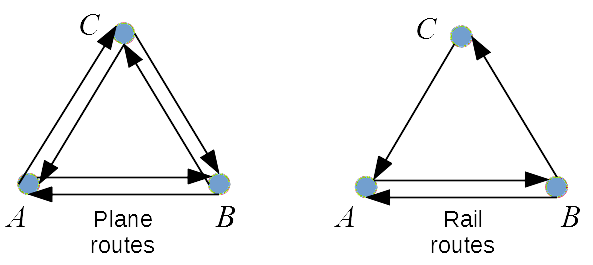
\includegraphics[width=2.5in]{relation-graphs.png}
%{\em Figure 1: Diagrams with Transport Links.}
\end{center}
\vspace{-10pt}
They have these following truth tables:
\begin{center}
\begin{tabular}{c|ccc}
Plane & $A$ & $B$ & $C$ \\ \hline
$A$ & $\mathtt{F}$ & $\mathtt{T}$ & $\mathtt{T}$ \\
$B$ & $\mathtt{T}$ & $\mathtt{F}$ & $\mathtt{T}$ \\
$C$ & $\mathtt{T}$ & $\mathtt{T}$ & $\mathtt{F}$
\end{tabular}
\hspace{2ex}
\begin{tabular}{c|ccc}
Rail & $A$ & $B$ & $C$ \\ \hline
$A$ & $\mathtt{F}$ & $\mathtt{T}$ & $\mathtt{F}$ \\
$B$ & $\mathtt{T}$ & $\mathtt{F}$ & $\mathtt{T}$ \\
$C$ & $\mathtt{T}$ & $\mathtt{F}$ & $\mathtt{F}$
\end{tabular}
\end{center}
Find the truth values of these statements:\\
{\bf (a)} $\forall x \exists y, \neg \mathrm{Plane}(x,y)$\\
{\bf (b)} $\forall x \forall y \exists z, \mathrm{Plane}(x,z) \wedge \mathrm{Plane}(z,y)$\\
{\bf (c)} $\exists x \exists y \exists z, \mathrm{Rail}(x,y) \wedge \mathrm{Rail}(y,z) \wedge \mathrm{Rail}(z,x)$\\
{\bf (d)} $\forall x \forall y \exists z, \mathrm{Rail}(x,z) \wedge \mathrm{Rail}(z,y)$\\
{\em Note.} In the truth tables the first argument is
represented by row, the second is represented by column. 
For example, $\mathrm{Rail}(\mathtt{C}, \mathtt{B}) = \mathtt{F}$ (3rd row,
2nd column).



{\bf Question 7.} 
Two positive real numbers $x,y \in \mathbb{R}^{+}$ are given. 
Translate into predicate logic this statement:
``Values $x$ and $y$ are the same, if we round them to two 
decimal places.'' Use variable names, arithmetic operations and 
the floor function ($\lfloor x \rfloor$ is the largest integer not
exceeding $x$).\\
{\em Note.} Rounding $x$ to two decimal places finds the 
number $\frac{p}{100}$ closest to $x$. 
If two are equally close, then round up.
(For example, $3.14159$ rounds to $3.14$; $3.144999$ rounds to $3.14$, 
but $3.145$ rounds to $3.15$.)\\
{\scriptsize \em (Write predicate expression; specify domains for quantifiers)}\\
\framebox(220,30){}

\newpage

\section{Answers}

{\bf Question 1:} Answer: Number $n \in \mathbb{Z}^{+}$ is a {\em prime} iff
\begin{align}
P(n) & :=\, \forall d \in \mathbb{Z}^{+}, \nonumber \\
 & \left( n > 1 \wedge \left( d \,\mid\, n \;\rightarrow\; (d = 1 \vee d = n) \right)\right). \nonumber
\end{align}
It is essential to require that $d$ is positive: $d \in \mathbb{Z}^{+}$, since prime numbers
may have negative divisors, say $n=7$ is divisible by four numbers: $d=-7, -1, 1, 7$. It is 
simpler to deal with only positive $d$ such that $d\,\mid\,n$.\\
Also it is essential that $n>1$; otherwise $n=1$ would also turn out to be a prime. Which is wrong, since it 
only has one divisor, not {\bf exactly} two.

\vspace{10pt}
{\bf Question 2:} Answer:\\[5pt]
\framebox(220,20){
$\forall N \in \mathbb{Z}^{+}\; \exists p \in \mathbb{Z}^{+},\;\left( p > N \,\wedge\, P(p) \right).$
}
In the predicate language this is a statement that for any (arbitrarily large) positive integer $N$ 
there exists an even larger positive integer $p$ such that $p$ is a prime. 

\vspace{10pt}
{\bf Question 3:} Answer:\\[5pt]
\framebox(220,20){
$(p \wedge q \wedge r) \vee (\neg p \wedge q \wedge \neg r) \vee (\neg p \wedge \neg q \wedge \neg r).$
}
For each row, where the truth table has value ${\tt T}$, we write one more
subexpression. Since there are just $3$ such rows in the table, 
there should be a disjunction $(\ldots) \vee (\ldots) \vee (\ldots)$. 
For example, the 2nd term $(\ldots)$ corresponds to the case, where $p = \mathtt{F}$, 
$q = \mathtt{T}$, $r = \mathtt{F}$, so we write $(\neg p \wedge q \wedge \neg r)$ (and other cases
are treated similarly).

\vspace{10pt}
{\bf Question 4:} {\bf (a)} Answer:\\[5pt]
\framebox(220,20){
$G\,:\, \{ 1,\ldots,10\} \times \{ 1,\ldots,10\} 
\,\rightarrow\, \{ \mathtt{T}, \mathtt{F} \}$.
}
Note that the predicate $G(i,j)$ acts not on the sets of children and hats, but 
on their {\em numbers}. Both $i$ and $j$ change over the same set $\{ 1,\ldots,10\}$.\\
{\bf (b)} Answer:\\[5pt]
\framebox(220,20){
$\forall i \in \{ 1,\ldots,10\}\; \forall j \in \{ 1,\ldots,10\},\; \,\left( G(i,j) \rightarrow i \neq j \right).$
}
{\em Note.} From the problem statement, some other predicate logic statements follow.
For example, we could also write another predicate logic statement saying that no child 
grabbed more than $1$ hat and every hat was taken. It is not wrong to add such clauses, 
but there were not part of the requirement of the problem, so the above answer is the 
simplest possible.

\vspace{10pt}
{\bf Question 5:} 
{\bf (a)} In the interval of real numbers $(0;1)$ there is no smallest number:\\[5pt]
\framebox(220,20){
$\forall x_1 \in (0;1)\, \exists x_2 \in (0;1),\, \left( x_2 < x_1 \right)$.
}\\
In this example the domain is $(0;1)$. It has no smallest number, since for every positive $x_1 > 0$
there exists an even smaller positive number. For example, we can take $x_2 = x_1/2$.\\
{\bf (b)} For the function $f(x) = x^2 - x$ defined on $(0;1)$ there exists the smallest value.\\[5pt]
\framebox(220,20){
$\exists x_0 \in (0;1)\,\forall x \in (0;1),\,\left( f(x) \geq f(x_0) \right)$.
}
In this case $f(x_0)$ is the smallest value, which is reached for the argument $x_0$. 
By the way, in our specific case this predicate logic statement is true. 
We can take $x_0 = \frac{1}{2} \in (0;1)$. This value gives the smallest value to 
the quadratic function $f(x) = x^2 - x$. But predicate logic statement can be written for 
any function $f(x): (0;1)\rightarrow \mathbb{R}$: 
If it does not have the minimum on $(0;1)$, the statement would be false.


\vspace{10pt}
{\bf Question 6:} Answers:\\
{\bf (a)} $\forall x \exists y, \neg \mathrm{Plane}(x,y) = \mathtt{True}$.\\
Indeed, for each city $x$ there is a city $y$ such that there is no plane connection. You can take $x = y$ (no 
plane goes from $x = A$ $x=B$, or $x=C$ to itself).\\
{\bf (b)} $\forall x \forall y \exists z, \mathrm{Plane}(x,z) \wedge \mathrm{Plane}(z,y)  = \mathtt{True}$.\\
Reasoning with $3$ variables and truth tables is not too convenient, but we can reason in plain English:
Is it true that for every two cities $x$ and $y$ (possibly $x = y$), there exists a city $z$, so that
one can fly from $x$ to $y$ via $z$? This is true and visible from the triangle graph.\\
{\bf (c)} $\exists x \exists y \exists z, \mathrm{Rail}(x,y) \wedge \mathrm{Rail}(y,z) \wedge \mathrm{Rail}(z,x) = \mathtt{True}$.\\
There exists a circular trip with rail. For example, we can take $(x,y,z) = (A,B,C)$. Then we can go from $A$ to $B$, 
$B$ to $C$ and $C$ to $A$.\\
{\bf (d)} $\forall x \forall y \exists z, \mathrm{Rail}(x,z) \wedge \mathrm{Rail}(z,y)= \mathtt{False}$.\\
If we take cities $x = A$ and $x = B$, then there exists no two-leg trip from $A$ to $B$ going through some city $z$.\\

\vspace{10pt}
{\bf Question 7:} Answer:\\[5pt]
\framebox(220,30){
${\displaystyle \left\lfloor 100x + \frac{1}{2} \right\rfloor = \left\lfloor 100y + \frac{1}{2} \right\rfloor}$. 
}
The fact that two numbers (for example, expressing money) round to exactly the same number
of euros and eurocents, can be written without any quantifiers. It is a predicate:
$P(x,y)$, with $P\,:\,\mathbb{R}^{+} \times \mathbb{R}^{+} \rightarrow \{ \mathtt{T},\mathtt{F} \}$.\\
{\em Note.} We could also write this with quantifiers. For example:
for the given $x,y$ there exists a non-negative integer number $z \in \mathbb{Z}^{0+}$ ($z$ expresses 
the number of eurocents) such that both $\left| 100x - z \right| \leq 0.5$ and $\left| 100y - z \right| \leq 0.5$. 
But writing such an expression would be longer, since we need to sort out the special case, when 
exactly one half of a eurocent ($x = 0.005$) is rounded up.










\end{document}



%%%%%%%%%%%%%%%%%%%%%%%%%%%%%%%%%%%%%%%%
%% End of RBS stuff
%%%%%%%%%%%%%%%%%%%%%%%%%%%%%%%%%%%%%%%%


%% 
%% Copyright (C) 2011-2017 by Brian D. Beitzel <brian at beitzel.com>
%% 
%% This work may be distributed and/or modified under the
%% conditions of the LaTeX Project Public License (LPPL), either
%% version 1.3c of this license or (at your option) any later
%% version.  The latest version of this license is in the file:
%% 
%% http://www.latex-project.org/lppl.txt
%% 
%% Users may freely modify these files without permission, as long as the
%% copyright line and this statement are maintained intact.
%% 
%% This work is not endorsed by, affiliated with, or probably even known
%% by, the American Psychological Association.
%% 
%% 
%% This work is "maintained" (as per LPPL maintenance status) by
%% Brian D. Beitzel.
%% 
%% This work consists of the file  apa6.dtx
%% and the derived files           apa6.ins,
%%                                 apa6.cls,
%%                                 apa6.pdf,
%%                                 README,
%%                                 APAamerican.txt,
%%                                 APAbritish.txt,
%%                                 APAdutch.txt,
%%                                 APAenglish.txt,
%%                                 APAgerman.txt,
%%                                 APAngerman.txt,
%%                                 APAgreek.txt,
%%                                 APAczech.txt,
%%                                 APAturkish.txt,
%%                                 APAendfloat.cfg,
%%                                 apa6.ptex,
%%                                 TeX2WordForapa6.bas,
%%                                 Figure1.pdf,
%%                                 shortsample.tex,
%%                                 longsample.tex, and
%%                                 bibliography.bib.
%% 
%%
%% End of file `./samples/shortsample.tex'.


\newpage
\documentclass[jou]{apa6}

\usepackage[american]{babel}

\usepackage{csquotes}
\usepackage[style=apa,sortcites=true,sorting=nyt,backend=biber]{biblatex}
\DeclareLanguageMapping{american}{american-apa}
\addbibresource{bibliography.bib}


%%%%%%%%%%%%%%%%%%%%%%%%%%%%%%%%%%%%%%%%
%% Discrete Structures
%% The start of RBS stuff
%%%%%%%%%%%%%%%%%%%%%%%%%%%%%%%%%%%%%%%%

% Working internal and external links in PDF
\usepackage{hyperref}
% Extra math symbols in LaTeX
\usepackage{amsmath}
\usepackage{gensymb}
\usepackage{amssymb}
% Enumerations with (a), (b), etc.
\usepackage{enumerate}

\let\OLDitemize\itemize
\renewcommand\itemize{\OLDitemize\addtolength{\itemsep}{-6pt}}

\usepackage{etoolbox}
\makeatletter
\preto{\@verbatim}{\topsep=3pt \partopsep=3pt }
\makeatother

% These sizes redefine APA for A4 paper size
\oddsidemargin 0.0in
\evensidemargin 0.0in
\textwidth 6.27in
\headheight 1.0in
\topmargin -24pt
\headheight 12pt
\headsep 12pt
\textheight 9.19in

\usepackage{xcolor}

\title{Sample Quiz 3}
\author{Discrete Structures, Fall 2020}
\affiliation{RBS}

\leftheader{Discrete Sample Quiz 3}

\abstract{%
}

%\keywords{}

\begin{document}

\twocolumn

\section{Worksheet 3: First Order Logic}


\vspace{6pt}
{\bf Question 1.} {\em Definition.} A Boolean formula is a 
{\em Conjunctive Normal Form (CNF)}, 
if it is a conjunction of one or more clauses, 
where a clause is a disjunction of literals. Each literal 
is either a variable ($u,v,\ldots$) or its negation ($\neg u, \neg v, \ldots$). 

Find the CNF computing the following truth table for Boolean 
expression $E(a,b,c)$:\\
\begin{tabular}{ c | c | c | c }
$a$ & $b$ & $c$ & $E(a,b,c)$  \\ \hline
{\tt T} & {\tt T} & {\tt T} & {\tt T} \\ \hline
{\tt T} & {\tt T} & {\tt F} & {\tt F} \\ \hline
{\tt T} & {\tt F} & {\tt T} & {\tt F} \\ \hline
{\tt T} & {\tt F} & {\tt F} & {\tt F} \\ \hline
{\tt F} & {\tt T} & {\tt T} & {\tt T} \\ \hline
{\tt F} & {\tt T} & {\tt F} & {\tt F} \\ \hline
{\tt F} & {\tt F} & {\tt T} & {\tt F} \\ \hline
{\tt F} & {\tt F} & {\tt F} & {\tt T} \\ \hline
\end{tabular}




\vspace{6pt}
{\bf Question 2.} The following CNF is given:
$$E = (a \vee \neg c) \wedge (b \vee \neg b).$$
Find $2$ Boolean expressions equivalent to $E$:\\[3pt]
{\bf (A)} $a \rightarrow \neg b$,\\[3pt]
{\bf (B)} $a \rightarrow c$,\\[3pt]
{\bf (C)} $\neg c \rightarrow \neg a$,\\[3pt]
{\bf (D)} $(a \wedge c) \rightarrow b$,\\[3pt]
{\bf (E)} $c \rightarrow a$,\\[3pt]
{\bf (F)} $a \rightarrow (c \rightarrow b)$,\\[3pt]
{\bf (G)} $\neg a \rightarrow \neg c$.

\vspace{6pt}
{\bf Question 3.} We have six statements about Python programs $p \in \mathcal{P}$
that convert inputs $i \in \mathbb{Z}^{+}$ into results $r \in \mathbb{Z}^{+}$.  
A Python program may either loop indefinitely or halt (i.e.\ it eventually stops).

\begin{enumerate}
\item Some programs return the correct result for all possible inputs and 
they never loop indefinitely.
\item For any program one can find another program such that it returns
the same result for the same inputs as the first one (or loops indefinitely, 
{\color{red} \bf iff} the first program does the same).
\item There is a program that only loops indefinitely for at most finitely many inputs (or maybe none at all), 
but for all other inputs it produces the correct result.
\item There is at least one Python program that always halts, and for sufficiently large inputs it produces
the correct result, but it may err for some small-size inputs.
\item For a program to produce a correct result for some input $i$ it is strictly necessary to halt.\\
\item A Python program always produces exactly one result for the given input provided that it halts.
\end{enumerate}

We use these $3$ predicates:\\
$A(p_1,i_2,r_3)$ is true iff
Python program $p_1 \in \mathcal{P}$ receives input $i_2 \in \mathbb{Z}^{+}$ and outputs 
result $r_3 \in \mathbb{Z}^{+}$.\\
$H(p_1,i_2)$ is true iff program $p_1 \in \mathcal{P}$ receives input $i_2$ and halts (i.e.\ does not
loop indefinitely).\\
$C(i_1,r_2)$ is true iff for input $i_1$ the correct result is $r_2$. 

{\em Note.} Write your answer as a comma-separated list: For example, 
{\tt F,E,D,C,B,A} tells that the 1st statement is {\bf (F)}, the 2nd one
is {\bf (E)}, $\ldots$, the last one is {\bf (A)}.


\begin{enumerate}[(A)]
\item ${\displaystyle \forall p \in \mathcal{P}\; \forall i \in \mathbb{Z}^+\; \forall r \in \mathbb{Z}^+,}$\\
${\displaystyle \left( A(p,i,r) \wedge C(i,r) \,\rightarrow\, H(p,i) \right) }$.
\item ${\displaystyle \forall p_1 \in \mathcal{P}\; \exists p_2 \in \mathcal{P}\;
\forall i \in \mathbb{Z}^{+}\; \textcolor{red}{\forall r \in \mathbb{Z}^{+},}}$\\
${\displaystyle \left( (\neg H(p_1,i) \wedge \neg H(p_2,i)) \vee 
(A(p_1,i,r) \leftrightarrow A(p_2,i,r)) \right)}$
\item ${\displaystyle \exists p \in \mathcal{P}\; \exists N \in \mathbb{Z}^{+}\; 
\forall i \in \mathbb{Z}^{+}\; \textcolor{red}{\exists r \in \mathbb{Z}^{+}},}$\\
${\displaystyle \left( ( i \leq N \wedge \neg H(p,i) ) \vee (A(p,i,r) \wedge C(i,r)) \right)}$.
\item ${\displaystyle \forall p \in \mathcal{P}\; \forall i \in \mathbb{Z}^{+}\; \forall r_1 \in \mathbb{Z}^{+}\;
\forall r_2 \in \mathbb{Z}^{+},}$\\ 
${\displaystyle \left( H(p,i) \wedge A(p,i,r_1) \wedge  A(p,i,r_2) \,\rightarrow\, r_1 = r_2 \right)}$.
\item ${\displaystyle \exists p \in \mathcal{P}\; \exists N \in \mathbb{Z}^{+}\; \forall i \in \mathbb{Z}^{+}\;
\textcolor{red}{\forall r \in \mathbb{Z}^{+}},}$\\
${\displaystyle \left( H(p,i) \,\wedge\, ( A(p,i,r) \wedge (i > N) \,\rightarrow\, C(i,r) ) \right)}$.
\item ${\displaystyle \exists p \in \mathcal{P}\; \forall i \in \mathbb{Z}^{+}\; \forall r \in \mathbb{Z}^{+},}$\\
${\displaystyle \left( H(p,i) \,\wedge\, (A(p,i,r) \rightarrow C(i,r) \right)}$. 
\end{enumerate}



\vspace{10pt}
{\bf Question 4.} There is a set of $4$ students $S = \{ s_1, s_2, s_3, s_4 \}$ and 
a set of $2$ chairs $C = \{ c_1, c_2 \}$. 
Find, how many such functions $f\,:\,S \rightarrow C$ exist, 
how many of them are injective, surjective and bijective.\\
{\em Note.} Your answer should be a comma-separated list of 
4 numbers (and 3 commas): {\tt total,injective,surjective,bijective}.


\vspace{10pt}
{\bf Question 5.}
There is a predicate $S(x, y, z)$ defined for triplets
of positive integers, 
$S: \mathbb{Z}^{+} \times \mathbb{Z}^{+} \times \mathbb{Z}^{+} \rightarrow \{ \mathtt{T}, \mathtt{F} \}$. 
$S(x,y,z)$ is true iff $x \cdot y = z$.\\
Express these statements about positive integers
using only $S(x,y,z)$, Boolean operations and quantifiers.\\
{\em Note.} Please use only the predicate $S(\ldots)$ in your answers, 
avoid any other predicates or relations (such as equality, divisibility, etc.).

\begin{enumerate}[(A)] 
\item $x/y = z$,
\item $x = 1$,
\item $x = y$, 
\item $x$ is divisible by $y$ (i.e. $y \,\mid\, x$). 
\item $x$ has odd number of positive divisors.
\item $x$ is not a prime.
\item $x$ is a prime.
\end{enumerate}




\subsection{Answers}

\vspace{6pt}
{\bf Question 1.} Answer: 
\begin{align}
 & \textcolor{red}{(\neg a \vee \neg b \vee c)} \wedge 
\textcolor{blue}{(\neg a \vee b \vee \neg c)} \wedge 
\textcolor{blue}{(\neg a \vee b \vee c)} \;\wedge \nonumber \\
\wedge\; & \textcolor{red}{(a \vee \neg b \vee c)} \wedge 
(a \vee b \vee \neg c) \nonumber
\end{align}
Every value {\tt F} in the truth table produces one 
clause in this expression. For example $E(\mathtt{T},\mathtt{T},\mathtt{F}) = \mathtt{F}$
is addressed by a disjunction $(\neg a \vee \neg b \vee c)$. 

If we combine red and blue clauses, we can rewrite this into a more compact expression, 
which is also CNF. Note, that this is not the only way to rewrite:
$$\textcolor{red}{(\neg b \vee c)} \wedge 
\textcolor{blue}{(\neg a \vee b)} \wedge
(a \vee b \vee \neg c).$$

\vspace{6pt}
{\bf Question 2.} Answer: {\bf (E)}, {\bf (G)}.\\
$(a \vee \neg c) \wedge (b \vee \neg b) = (a \vee \neg c) \wedge \mathtt{T} = (a \vee \neg c)$. 
This is same as $c \rightarrow a$ or the contrapositive variant of the same implication:
$\neg a \rightarrow \neg c$.

\vspace{6pt}
{\bf Question 3.} Answer:\\
\begin{tabular}{|c|c|c|c|c|c|} \hline
1 & 2 & 3 & 4 & 5 & 6 \\ \hline
{\bf (F)} & {\bf (B)} & {\bf (C)} & {\bf (E)} & {\bf (A)} & {\bf (D)} \\ \hline
\end{tabular} 

\vspace{3pt}
In {\bf (B)} we should write: the second program loops indefinitely {\bf iff} 
the first program does so. If we write {\bf if} instead, it 
would mean only one-way conditional, which does not mean 
equivalence between the programs $p_1$ and $p_2$, but something more complicated.

In {\bf (B)} you could write $(H(p_1,i) \leftrightarrow H(p_2,i))$
instead of $(\neg H(p_1,i) \wedge \neg H(p_2,i))$ or 
even omit any reference to $H(\ldots)$ predicates. 
The notation $(H(p_1,i) \leftrightarrow H(p_2,i))$ stresses the fact that $p_1$ and $p_2$ behave in the same way. 
But in fact the equivalence $(A(p_1,i,r) \leftrightarrow A(p_2,i,r))$ implicitly 
states the fact that $p_1$ and $p_2$ are defined on the same inputs.

Please note that {\bf (B)} should {\bf NOT} have quantifier  
 $\textcolor{red}{\exists r \in \mathbb{Z}^{+}}$ 
(instead of  $\textcolor{red}{\forall r \in \mathbb{Z}^{+}}$), because we need
equivalence for all positive integers $r$. If we only care about the
actual result of $p$ on input $i$, then it is possible to ``cheat'' the logic formula: 
pick result $r$ which is impossible for both $p_1$ and $p_2$; then $A(p_1,i,r)$ 
and $A(p_2,i,r)$ would both be false (and thus equivalent).

In {\bf (C)} one cannot replace $\textcolor{red}{\exists r \in \mathbb{Z}^{+}}$
with $\textcolor{red}{\forall r \in \mathbb{Z}^{+}}$ (as in an earlier draft of this test), 
because it does not make sense to ask that a program $p$ on input $i$ produces
{\bf each} positive integer result; and all results turn out to be correct. 
(Such a formula may have some useful meaning if predicates $A,H,C$ have different
interpretations, but for Python programs this is technically correct, but 
has an absurd meaning: that a given program produces any result whatsoever.)

In {\bf (E)} it is absolutely necessary to write a quantifier 
$\textcolor{red}{\forall r \in \mathbb{Z}^{+}}$, because 
leaving $r$ as a free variable (without a quantifier) would 
mean that the Python program always produces the same result
(the value of $r$). It is not 


\vspace{6pt}
{\bf Question 4.} Answer: {\tt 16,0,14,0}\\
Please note that there can be no injections (and therefore also bijections): 
students will always collide \textendash{} run to the same chair, 
since there are fewer chairs than students.

The total number of functions is $2^4 = 16$. Each student
can choose between $2$ chairs, so it is $2 \times 2 \times 2 \times 2 = 16$. 
Moreover, there are only $2$ ``constant'' functions (where all four
students go to $c_1$ or to $c_2$). They are not surjective, because
some chairs stay unoccupied in this case. 
All the other $16 - 2 = 14$ functions from $S$ (4 elements) to $C$ (2 elements)
are surjections. 

\vspace{6pt}
{\bf Question 5.} Here we write all $7$ statements with predicate $S(x,y,z)$ and quantifiers. 

\begin{enumerate}[(A)]
\item $S(z,y,x)$ (or, equivalently, $S(y,z,x)$). 
\item $\exists y \in \mathbb{Z}^{+},\; S(x,y,y)$.\\
Use the property: $x = 1$ can multiply with an $y$, and does not increase/decrease. \\
You could also write simply $S(x,x,x)$. Indeed, $x$ is the only 
positive integer such that $x \cdot x = x$. (Allowing $x = 0$ would 
spoil this, because $0^2 = 0$.)
\item $\exists z \in \mathbb{Z}^{+},\; S(x,z,y) \wedge S(z,z,z)$.\\
So, $x = y$ iff there is a $z = 1$ such that $x \cdot z = y$.
\item $\exists d \in \mathbb{Z}^{+},\; S(y,d,x)$.
\item $\exists y \in \mathbb{Z}^{+},\; S(y,y,x)$.\\ 
This means that $y^2 = x$ for some $y$; 
hence $x$ is a full square and should have odd number of divisors.
\item $\exists y \in \mathbb{Z}^{+}\;\exists z \in \mathbb{Z}^{+},\;(S(y,z,x) \wedge \neg S(y,y,y) \wedge \neg S(z,z,z))$.\\
This means that a non-prime $x$ can be expressed as a product of two positive integers $y,z$, 
where neither of them is $1$.)
\item $\forall y \in \mathbb{Z}^{+}\;\forall z \in \mathbb{Z}^{+},\;(\neg S(y,z,x) \vee S(y,y,y) \vee S(z,z,z))$.\\
We apply negation to the previous quantifier formula; all $\exists$ quantifiers turn into $\forall$; 
formulas are changed according to De Morgan's laws.
\end{enumerate}










\end{document}




\newpage
\documentclass[jou]{apa6}

\usepackage[american]{babel}

\usepackage{csquotes}
\usepackage[style=apa,sortcites=true,sorting=nyt,backend=biber]{biblatex}
\DeclareLanguageMapping{american}{american-apa}
\addbibresource{bibliography.bib}


%%%%%%%%%%%%%%%%%%%%%%%%%%%%%%%%%%%%%%%%
%% Discrete Structures
%% The start of RBS stuff
%%%%%%%%%%%%%%%%%%%%%%%%%%%%%%%%%%%%%%%%

% Working internal and external links in PDF
\usepackage{hyperref}
% Extra math symbols in LaTeX
\usepackage{amsmath}
\usepackage{gensymb}
\usepackage{amssymb}
% Enumerations with (a), (b), etc.
\usepackage{enumerate}

\let\OLDitemize\itemize
\renewcommand\itemize{\OLDitemize\addtolength{\itemsep}{-6pt}}

\usepackage{etoolbox}
\makeatletter
\preto{\@verbatim}{\topsep=3pt \partopsep=3pt }
\makeatother

% These sizes redefine APA for A4 paper size
\oddsidemargin 0.0in
\evensidemargin 0.0in
\textwidth 6.27in
\headheight 1.0in
\topmargin -24pt
\headheight 12pt
\headsep 12pt
\textheight 9.19in

\usepackage{xcolor}


\title{Quiz for Week02}
\author{Discrete Structures, Fall 2020}
\affiliation{RBS}

\leftheader{Discrete Structures (W2): Quiz}

\abstract{%
}

%\keywords{}

\begin{document}

\twocolumn

\section{Quiz 3: First Order Logic}




\vspace{6pt}
{\bf Question 1.} We have the following
truth table. 
Find the correct DNF (Disjunctive Normal Form) expressing $E(X,Y,Z)$.\\
{\em Note.} Multiple answers may be true, since
there may more than one way to write DNFs for the same Boolean 
function.


\begin{tabular}{@{}ll@{}} 
\begin{minipage}{0.33\columnwidth}
\noindent
\begin{tabular}{ c | c | c | c }
$X$ & $Y$ & $Z$ & $E$ \\ \hline
{\tt T} & {\tt T} & {\tt T} & {\tt F} \\ \hline
{\tt T} & {\tt T} & {\tt F} & {\tt F} \\ \hline
{\tt T} & {\tt F} & {\tt T} & {\tt T} \\ \hline
{\tt T} & {\tt F} & {\tt F} & {\tt F} \\ \hline
{\tt F} & {\tt T} & {\tt T} & {\tt T} \\ \hline
{\tt F} & {\tt T} & {\tt F} & {\tt F} \\ \hline
{\tt F} & {\tt F} & {\tt T} & {\tt T} \\ \hline
{\tt F} & {\tt F} & {\tt F} & {\tt F} \\ \hline
\end{tabular}
\end{minipage} &
\begin{minipage}{0.65\columnwidth}

\begin{enumerate}[(A)]
\item $(X \wedge \neg Y \wedge Z) \;\vee\;$\\
$\;\vee\; (\neg X \wedge Y \wedge Z)$.
\item $(\textcolor{red}{\neg X} \wedge Y \wedge Z) \vee (\neg Y \wedge Z)$.
\item $(\neg X \wedge Z) \vee (X \wedge \neg Y \wedge Z)$.
\item $(\neg X \wedge \neg Y \wedge Z) \vee (\neg X \wedge Y)$.
\end{enumerate}

\end{minipage}
\end{tabular}


\vspace{6pt}
{\bf Question 2.} Identify, which is the correct CNF 
(Conjunctive Normal Form) that computes the same thing as 
Peirce's arrow: $a \downarrow b = \neg (a \vee b)$.\\
{\em Note.} Multiple answers may be true, since
there may more than one way to write CNFs for the same Boolean 
function.

\noindent
{\normalsize \bf (A)} %% Fine
$(\neg a \vee \neg b) \wedge (\neg a \vee b) \wedge (a \vee \neg b)$.\\[3pt]
{\normalsize \bf (B)}
$(a \vee b) \wedge (\neg a \vee b) \wedge (a \vee \neg b)$.\\[3pt]
{\normalsize \bf (C)}
$\neg a \vee \neg b$.\\[3pt]
{\normalsize \bf (D)} %% Fine
$\neg a \wedge (a \vee \neg b)$.



\vspace{6pt}
{\bf Question 3.} We have predicates $A(p,i,r)$ (a Python program 
$p \in \mathcal{P}$ receives input $i \in \mathbb{Z}^{+}$ and answers
with the result $r \in \mathbb{Z}^{+}$); $H(p,i)$ (program $p$ halts on input $i$), 
and $C(i,r)$ (the correct/expected output for input $i$ is $r$). 
Identify the predicate expression that expresses the following English sentence:

{\em ``For all inputs that are sufficiently large, the given program $p$ 
halts and produces outputs that are correct; for some (finitely many) inputs $p$ 
may loop forever, but it is never incorrect.''}




\noindent
{\normalsize \bf (A)}
$\forall p \in \mathcal{P}\; \forall i \in \mathbb{Z}^{+}\; \forall r \in \mathbb{Z}^{+},$\\
$((i > M \,\wedge\, H(p,i)) \vee (A(p,i,r) \wedge C(i,r)))$.\\[3pt]
{\normalsize \bf (B)}
$\exists M \in \mathbb{Z}^{+}\; \forall i \in \mathbb{Z}^{+}\;
\exists r \in \mathbb{Z}^{+},$\\
$((i < M \,\wedge\, \neg H(p,i)) \vee (A(p,i,r) \wedge C(i,r)))$.\\[3pt]
{\normalsize \bf (C)}
$\forall p \in \mathcal{P}\; \exists M \in \mathbb{Z}^{+}\; \forall i \in \mathbb{Z}^{+}\;
\forall r \in \mathbb{Z}^{+},$\\
$((i > M \,\wedge\, H(p,i)) \vee (A(p,i,r) \wedge C(i,r)))$.\\[3pt]
{\normalsize \bf (D)}
$\forall p \in \mathcal{P}\; \forall i \in \mathbb{Z}^{+}\;
\forall r \in \mathbb{Z}^{+},$\\
$((i > M \,\wedge\, H(p,i)) \vee (A(p,i,r) \wedge C(i,r)))$.


\vspace{6pt}
{\bf Question 4.} For the quantifiers 
($A(p,i,r)$, $H(p,i)$, $C(i,r)$) defined in the previous question, 
the following expression is given:
$$\forall p \in \mathcal{P}\;
\exists i \in \mathbb{Z}^{+}\; \exists j \in \mathbb{Z}^{+},$$
$$(j > i \,\wedge\, (H(p,i) \rightarrow H(p,j)).$$
Which sentence is expressed by this?

\noindent
{\bf (A)} Each Python program halts for at least 2 inputs.\\
{\bf (B)} Each Python program halts for infinitely many inputs. \\
{\bf (C)} There is no Python program that halts on exactly 1 input. \\
{\bf (D)} For each Pyton program there is the largest input for which it halts.\\
{\color{red} {\bf (E)} The statement is always true (regardless of halting behavior of Python programs).}

\vspace{6pt}
{\bf Question 5.} 
There is a set of 2 students $S = \{ s_1, s_2 \}$ and 
a set of 5 chairs $C = \{ c_1, c_2, c_3, c_4, c_5 \}$. 
Find, how many such functions $f\,:\,S \rightarrow C$ exist (a function 
by definition is a mapping that assigns a chair for each student;
it is NOT always true that different students get different chairs
or that all chairs are occupied). Please find the total number of 
such functions, also the number of injective, surjective
and bijective functions among them.\\
{\em Note.} Your answer should be a comma-separated list of 
4 numbers (and 3 commas).



\vspace{6pt}
{\bf Question 6.} 
Predicate $S(x,y,z)$ is true iff $x \cdot y=z$.
Given the following equation:\\[3pt]
$\forall u \in \mathbb{Z}^{+}\;\forall v \in \mathbb{Z}^{+}\;
\textcolor{red}{\forall d \in \mathbb{Z}^{+}}\;
\forall p \in \mathbb{Z}^{+}\;\forall q \in \mathbb{Z}^{+}\;
\exists k \in \mathbb{Z}^{+},$\\
$S(x,u,y) \wedge S(x,v,z) \wedge
S(d,p,y) \wedge S(d,q,z) \rightarrow S(d,k,x).$


Which statement is expressed by this expression?\\
{\bf (A)} $d$ is the greatest common divisor of $y$ and $z$,\\
{\bf (B)} $x$ is the greatest common divisor of $p$ and $q$,\\
{\bf (C)} $x$ is the greatest common divisor of $y$ and $z$,\\
{\bf (D)} $d$ is the greatest common divisor of $u$ and $v$.

\vspace{6pt}
{\bf Question 7.} 
\begin{center}
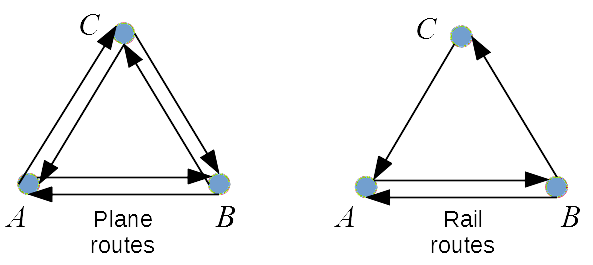
\includegraphics[width=2in]{relation-graphs.png}
\end{center}

Find the predicate expression that expresses this statement: 
"For the two given cities $x$ and $y$ there is a two-leg trip
using planes, but there is no two-leg trip using rail."\\
{\em Note.} We call a trip "two-leg", if it uses exactly two plane flights
or exactly two rail links. 
In this example all variables are from a 3-element set $\mathtt{City} = \{A,B,C\}$ 
\textendash{} see Figure. 


\noindent
{\bf (A)} $\forall x\;\forall y\; \forall z,\; \mathtt{Plane}(x,z) \wedge \mathtt{Plane}(z,y) \wedge$\\
$\neg \left( \mathtt{Rail}(x,z) \wedge \mathtt{Rail}(z,y) \right)$.\\[3pt]
{\bf (B)} $\exists z,\; \mathtt{Plane}(x,z) \wedge \mathtt{Plane}(z,y) \wedge$\\
$\neg \left(\mathtt{Rail}(x,z) \wedge \mathtt{Rail}(z,y)\right)$.\\[3pt]
{\bf (C)} $\forall x\; \forall y\; \exists z,\; \mathtt{Plane}(x,z) \wedge \mathtt{Plane}(z,x) \wedge$\\
$(\neg \mathtt{Rail}(x,z) \vee \neg \mathtt{Rail}(z,y))$.\\[3pt]
{\bf (D)} $\exists z_1\; \forall z_2,\; \mathtt{Plane}(x,z_1) \wedge \mathtt{Plane}(z_1,y) \wedge$\\
$(\neg \mathtt{Rail}(x,z_2) \vee \neg \mathtt{Rail}(z_2,y))$.





\subsection{Answers}

\vspace{6pt}
{\bf Question 1.} Answer {\bf (B),(C)}.\\
An obvious way to write DNF for this expression:
$$(X \wedge \neg Y \wedge Z) \vee (\neg X \wedge Y \wedge Z) \vee (\neg X \wedge \neg Y \wedge Z).$$
It contains one clause per every {\tt T} in the truth table. But it is not among the 
answers. Instead the answers {\bf (B)} and {\bf (C)} contain one shorter clause (with just two variables) that 
is equivalent to two clauses with three variables. For example, 
\begin{align}
 & (\neg Y \wedge Z) \equiv \nonumber \\
\equiv & \mathtt{True} \wedge (\neg Y \wedge Z) \equiv \nonumber \\
\equiv & (X \vee \neg X) \wedge (\neg Y \wedge Z) \equiv \nonumber \\
\equiv & (X \wedge (\neg Y \wedge Z)) \vee (\neg X \wedge (\neg Y \wedge Z)) \nonumber
\end{align}
Therefore the DNF can be written in a more compact form when we combine two blue clauses into
a shorter one:
$$\textcolor{blue}{(X \wedge \neg Y \wedge Z)} \vee (\neg X \wedge Y \wedge Z) \vee \textcolor{blue}{(\neg X \wedge \neg Y \wedge Z)} \equiv$$
$$\equiv \textcolor{blue}{(\neg Y \wedge Z)} \vee (\neg X \wedge Y \wedge Z)$$

\vspace{6pt}
{\bf Question 2.} Answer: {\bf (A)}, {\bf (D)}.\\
The variant {\bf (A)} lists all $3$ ways how $a \downarrow b$ can take value {\tt F}.\\
Variant {\bf (D)} $(\neg a) \wedge (a \vee \neg b)$ is the same thing. The clause $\textcolor{blue}{(\neg a)}$ 
there is equivalent to two clauses from {\bf (A)}: $\textcolor{blue}{(\neg a \vee \neg b) \wedge (\neg a \vee b)}$.

\vspace{6pt}
{\bf Question 3.} Answer: {\bf (B)}.\\
This means that there is a positive integer $M$ such that
for each $i \in \mathbb{Z}^{+}$ there would be $r \in \mathbb{Z}^{+}$ such that 
{\bf either} input $i$ is small ($i < M$) and program does not halt. 
{\bf Or} program $p$ outputs result $r$ upon receiving $i$ and 
that result is correct. (Note that even for small $i$ it is allowed
to stop and to output a correct answer: In this case $(i < M \,\wedge\, \neg H(p,i))$ is false, 
but $(A(p,i,r) \wedge C(i,r))$ is true.

Let us consider answer alternative {\bf (C)}:\\
$\forall p \in \mathcal{P}\; \exists M \in \mathbb{Z}^{+}\; \forall i \in \mathbb{Z}^{+}\;
\forall r \in \mathbb{Z}^{+},$\\
$((i > M \,\wedge\, H(p,i)) \vee (A(p,i,r) \wedge C(i,r)))$.

Note that for the answer {\bf (C)} (just like {\bf (A)} and {\bf (D)}) 
starts with $\forall p \in \mathcal{P}$. These statments contain 
$p$ as a {\em bound variable}; therefore they cannot express anything 
meaningful about the special $p$ mentioned in the English sentence: 
``For all inputs that are sufficiently large, {\bf the given program $p$}
halts and produces outputs.'' (The given Python program $p$ is not {\bf any program} or 
{\bf some program}; it is one certain program \textendash{} variable $p$ 
should have no quantifier.)

Even if we drop that $p \in \mathcal{P}$ the statement {\bf (C)} expresses 
something different: ``For a program there exists a number $M$ such that for all $i > M$ 
the program should halt. For any ``small'' input $i$ ($i \leq M$) it is not sufficient to halt; 
the program must be able to output {\bf any} result $r$ for the received input; 
and moreover \textendash{} that output should be correct:
$(A(p,i,r) \wedge C(i,r)))$.

\vspace{6pt}
{\bf Question 4.} Answer: {\bf (E)}.\\
Let us forget anything we know about Python programs and their halting. 
Let $H(p,i)$ be any predicate on elements of some set $p \in \mathcal{P}$ and  
positive integers $i$. We can prove that 
$(j > i \,\wedge\, (H(p,i) \rightarrow H(p,j))$ is always true. 
For the given $p$ take three different numbers $i_1,i_2,i_3$. Among 
$H(p,i_1)$, $H(p,i_2)$, $H(p,i_3)$ there are two values that are both true (or both false). 
Assign $i$ to the smallest of these $i_1,i_2,i_3$, and assign $j$ to the largest. 


\vspace{6pt}
{\bf Question 5.} Answer: {\tt 25,20,0,0}.\\
There are $5 \cdot 5 = 25$ ways to assign two students to five chairs
(you have to make a choice "1 of 5" two times).\\
Out of these $25$ functions there are $5$ functions that map both students
to the same chair ($c_1$, $c_2$, $c_3$, $c_4$, or $c_5$). All the other
$25-5 = 20$ functions that are injective (i.e. $f(s_1) \neq f(s_2)$).\\
Since there are more chairs than students, there are no surjective and bijective
functions.

\vspace{6pt}
{\bf Question 6.} Answer: {\bf (C)}.\\
The only option can be $x$ is the greatest common divisor of $y$ and $z$. 
$S(x,u,y)$ and $S(x,v,z)$ show that $x$ is {\bf some} common divisor of 
$y$ and $z$. And since $S(d,p,y) \wedge S(d,q,z) \rightarrow S(d,k,x)$ 
it means that another common divisor $d$ is also a divisor of $x$.\\
Therefore $x$ is the {\bf greatest} common divisor of $y$ and $z$. 

You can easily eliminate alternatives {\bf (B)}, {\bf (D)}, because
they state something about greatest common divisor of $p,q$ or $u,v$. 
But all these variables are {\bf bound} variables (they do not 
have any specific value; they vary over the whole set of positive integers). 


\vspace{6pt}
{\bf Question 7.} Answer: {\bf (D)}.\\
Note that the intermediate city $z_1$ for plane flights (that should exist)
has nothing common with the city $z_2$ for rail connections (that should not exist).
The conjunction {\bf BUT} means same as {\bf AND} from the logic point of view. 
We could express the answer like this:\\
$(\exists z_1,\; \mathtt{Plane}(x,z_1) \wedge \mathtt{Plane}(z_1,y))$ {\bf AND}\\
$\neg (\exists z_2,\; \mathtt{Rail}(x,z_2) \wedge \mathtt{Rail}(z_2,y))$. 

We can simpify the second clause using De Morgan's law:
$\forall z_2, (\neg \mathtt{Rail}(x,z_2) \vee \neg \mathtt{Rail}(z_2,y))$ and 
combine with the first clause by writing both quantifiers $\exists z_1$ and
$\forall z_2$ at the very front of the expression. 






\end{document}


\newpage
\documentclass[jou]{apa6}

\usepackage[american]{babel}

\usepackage{csquotes}
\usepackage[style=apa,sortcites=true,sorting=nyt,backend=biber]{biblatex}
\DeclareLanguageMapping{american}{american-apa}
\addbibresource{bibliography.bib}


%%%%%%%%%%%%%%%%%%%%%%%%%%%%%%%%%%%%%%%%
%% Discrete Structures
%% The start of RBS stuff
%%%%%%%%%%%%%%%%%%%%%%%%%%%%%%%%%%%%%%%%

% Working internal and external links in PDF
\usepackage{hyperref}
% Extra math symbols in LaTeX
\usepackage{amsmath}
\usepackage{gensymb}
\usepackage{amssymb}
% Enumerations with (a), (b), etc.
\usepackage{enumerate}

\let\OLDitemize\itemize
\renewcommand\itemize{\OLDitemize\addtolength{\itemsep}{-6pt}}

\usepackage{etoolbox}
\makeatletter
\preto{\@verbatim}{\topsep=3pt \partopsep=3pt }
\makeatother

% These sizes redefine APA for A4 paper size
\oddsidemargin 0.0in
\evensidemargin 0.0in
\textwidth 6.27in
\headheight 1.0in
\topmargin -24pt
\headheight 12pt
\headsep 12pt
\textheight 9.19in



\title{Sample Quiz 4}
\author{Discrete Structures, Fall 2020}
\affiliation{RBS}

\leftheader{Discrete Sample Quiz 4}

\abstract{%
}

%\keywords{}

\begin{document}

%\thispagestyle{empty}

\twocolumn
\section{Worksheet 4: Sets}

\vspace{10pt}
{\bf Question 1.} We define three sets in the universe $U$ of integer numbers
between $1$ and $70$ (inclusive):
$$\left\{ \begin{array}{rcl}
K_2 & = & \{ x \in U \,\mid\, 2 \mid x \},\\
K_5 & = & \{ x \in U \,\mid\, 5 \mid x \},\\
K_7 & = & \{ x \in U \,\mid\, 7 \mid x \},
\end{array} \right.$$

Find the size of the following sets.
Here $|X|$ denotes the number of elements in a finite set
(BTW, $|X|$ is also the notation for the cardinality of an infinite set).\\
{\em Note.} It was not intentional, but vertical bar: $\mid$
in this exercise happens to be used in three different ways: 
It is a separator when defining sets $K_2$; it is used to denote
divisibility; it also denotes set cardinality.

\begin{tabular}{ll} 
$\left| K_2 \cup K_5 \right|$ & $\ldots$ \\ 
$\left| K_2 \cap K_7 \right|$ & $\ldots$ \\ 
$\left| \overline{K_7} \right|$ & $\ldots$ \\
$\left| \overline{K_2 \cap K_5} \right|$ & $\ldots$ \\
$\left| K_2 \cap K_5 \cap K_7 \right|$ & $\ldots$ \\ 
$\left| K_2 \cap K_5 \cap \overline{K_7} \right|$ & $\ldots$ \\ 
$\left| K_2 \cup K_5 \cup K_7 \right|$ & $\ldots$ \\ 
$\left| \overline{K_2 \cup K_5 \cup K_7} \right|$ & $\ldots$ \\ 
\end{tabular}


\vspace{6pt}
{\bf Question 2.}
Find a counterexample to refute the following predicate expression:\\
$(\exists x \in U,\;P(x)) \wedge (\exists x\in U,\;Q(x)) \rightarrow$\\
$\rightarrow \exists x\in U,\;(P(x) \wedge Q(x))$.\\
Here $P(x)$ is true iff $P$ is a full square (a square of some integer number), 
$Q(x)$ is true iff $x$ is divisible by $5$, and $U$ is the set of all integers 
from the interval $[120;130]$.\\
{\em Note.} The three $x$'s in this formula refer to 
three unrelated (local) variables. 
If it looks confusing, you can rewrite it like this:\\
$(\exists x_1 \in U,\;P(x_1)) \wedge (\exists x_2\in U,\;Q(x_2)) \rightarrow$\\
$\rightarrow \exists x_3\in U,\;(P(x_3) \wedge Q(x_3))$.

\noindent
{\bf (A)} Identify the variables which you need to pick for your counter-example.\\
{\bf (B)} Pick the values for these variables to make the above statement false.


\vspace{6pt}
{\bf Question 3.} Determine the cardinality of the following sets (some finite number? 
equal to $|\mathbb{N}|$? equal to $|\mathcal{P}(\mathbb{N})| = |\mathbb{R}|$? equal to $|\mathcal{P}(\mathbb{R})|$?)
\begin{enumerate}[(A)]
\item The set of positive real numbers from $(0;1)$ with decimal representation 
containing only digits $0$ and $1$? 
\item The set of positive real numbers from $(0;1)$ with decimal representation 
containing only digits $0$ and $1$ (and it is known that the number of $0$s is finite)? 
\item The set of positive real numbers from $(0;1)$ that are fully periodic decimal fractions with 
a period of $2020$ digits? 
\item The set of positive real numbers from $(0;1)$ that have decimal representation 
without any digits "9"?
\item The set of all irrational $x \in (0;1)$ such that $x^3$ is rational?
\item Ordered pairs of real numbers $x_1,x_2$ such that $x_1,x_2 \in (0;1)$. 
\item Finite sequences of real numbers: $x_1,\ldots,x_n$, and all $x_i \in (0;1)$? (Here $n$ can 
be any positive integer)? 
\item Infinite sequences of real numbers from $(0;1)$: $\{ x_n \}$: $x_1,x_2,x_3,\ldots$.
\end{enumerate}


\vspace{6pt}
{\bf Question 4.}
Let ${\displaystyle f(x) = \left\lfloor \frac{x^3}{3} \right\rfloor}$. Find $f(S)$ if $S$ is:
\begin{enumerate}[(A)]
\item $S = \{ −2, −1, 0, 1, 2, 3 \}$.
\item $S = \{0, 1, 2, 3, 4, 5 \}$.
\item $S = \{1, 5, 7, 11 \}$.
\end{enumerate}
Is function $f: \mathbb{Z} \rightarrow \mathbb{Z}$ injective? Is it surjective? 
If it is not, mention counterexamples to show this. 

\vspace{6pt}
{\bf Question 5.}
Determine, if the given set is a powerset of some other set. If yes, which one?
\begin{enumerate}[(A)]
\item $\{\emptyset,\; \{\emptyset\},\; \{a\},\; \{\{a\}\},\; \{\{\{a\}\}\},\; \{\emptyset, a\},\; \{\emptyset, \{a\}\},\; \{\emptyset, \{\{a\}\}\},$\\
\mbox{}$\;\{a, \{a\}\},\; \{a, \{\{a\}\}\},\; \{\{a\}, \{\{a\}\}\},\; \{\emptyset, a, \{a\}\},\; \{\emptyset, a, \{\{a\}\}\},$\\
\mbox{}$\;\{\emptyset, \{a\}, \{\{a\}\}\},\; \{a, \{a\}, \{\{a\}\}\},\; \{\emptyset, a, \{a\}, \{\{a\}\}\}\}$.
\item $\{\emptyset, \{a\}\}$.
\item $\{\emptyset, \{a\}, \{\emptyset, a\}\}$.
\item $\{\emptyset, \{a\}, \{\emptyset\}, \{a, \emptyset\}\}$.
\item $\{\emptyset, \{a, \emptyset\}\}$.
\end{enumerate}

\vspace{6pt}
{\bf Question 6.}
Given two sets $A = \{ x, y \}$ and $B = \{x, \{x \}\}$, check, if statements are true or false:
\begin{enumerate}[(A)]
\item $x \subseteq B$.
\item $\emptyset \in \mathcal{P}(B)$.
\item $\{x\} \subseteq A - B$.
\item $|\mathcal{P}(A)| = 4$.
\end{enumerate}


\vspace{6pt}
{\bf Question 7.}
We define functions $g\,:\, A \rightarrow A$ and $f : A \rightarrow A$, where $A \{1, 2, 3, 4\}$ by 
listing all argument-value pairs: 
$$g = \{(1, 4), (2, 1), (3, 1), (4, 2)\},\;\;f = \{(1, 3), (2, 2), (3, 4), (4, 1)\}.$$
Find these functions by listing their argument/value pairs (or establish that they do not exist).
\begin{enumerate}[(A)]
\item Find $f \circ g$.
\item Find $g \circ f$.
\item Find $g \circ g$.
\item Find $g \circ (g \circ g)$.
\item Find $f^{-1}$.
\item Find $g^{-1}$.
\end{enumerate}


\vspace{6pt}
{\bf Question 8.} Find these sums:
\begin{enumerate}[(A)]
\item $1/4 + 1/8 + 1/16 + 1/32 + \ldots$.
\item $2 + 4 + 8 + 16 + 32 + \ldots + 2^{28}$.
\item $2 - 4 + 8 - 16 + 32 - \ldots - 2^{28}$.
\item $1 - 1/2 + 1/4 - 1/8 + 1/16 - \ldots$.
\end{enumerate}

\vspace{6pt}
{\bf Question 9.} Find an appropriate $O(g(n))$ for each function $f(n)$ defined below 
(pick your $g(n)$ to be the slowest growing among the functions such that $f(n)$ is in $O(g(n))$). 
\begin{enumerate}[(A)]
\item $f(n) = 1^2 + 2^2 + \ldots + n^2$.
\item ${\displaystyle f(n) = \frac{3n - 8 - 4n^3}{2n - 1}}$. 
\item ${\displaystyle f(n) = \sum\limits_{k=1}^{n} k^3}$.
\item ${\displaystyle f(n) = \frac{6n + 4n^5 - 4}{7n^2 - 3}}$. 
\item ${\displaystyle f(n) = \sum\limits_{k=2}^{n} k\cdot(k-1)}$.
\item ${\displaystyle f(n) = 3n^2 + 8n + 7}$
\end{enumerate}

\vspace{6pt}
{\bf Question 10.}
For the given functions, find an optimal $O(g(n))$; find
$C$ and $n_0$ (from the definition $|f(n)| < C\cdot |g(n)|$ as long as $n > n_0$). 
\begin{enumerate}[(A)]
\item ${\displaystyle f(n) = 3n^4 + \log_2 n^8}$. 
\item ${\displaystyle f(n) = \sum\limits_{k=1}^{n} (k^3 + k)}$.
\item ${\displaystyle f(n) = (n + 2)\log_2 (n^2 + 1) + \log_2 (n^3 + 1)}$.
\item ${\displaystyle f(n) = n^3 + \sin n^7}$.
\end{enumerate}


\vspace{6pt}
{\bf Question 11.} This is a Python fragment; variable {\tt n} can become very large; {\tt t} is some
fixed parameter. Denote by $f(n)$ the number of operations depending on the variable {\tt n}, 
where an operation is an addition or a multiplication, or raising to the power 2.
Find the slowest growing $g(n)$ so that $f(n)$ is in $O(g(n))$. 
\begin{verbatim}
sum = 0
for i in range(1,n+1):
    for j in range(1,n+1):
        sum += (i*t + j*t + 1)**2
\end{verbatim}

\vspace{6pt}
{\bf Question 12.} There are two functions $f,g: \mathbb{R} \rightarrow \mathbb{R}$ defined
for all real numbers and taking real values.
Find, which predicate logic expressions describe a statement that is logically
equivalent to the English sentence ``The function $f(n)$ is in $O(g(n))$''.\\
{\em Note.} There may be multiple correct answers. 

\begin{enumerate}[(A)]
\item $\forall n \in \mathbb{R}\;\exists n_0 \in \mathbb{R}\;\exists C \in \mathbb{R},$\\
$\left(n > n_0 \rightarrow |f(n)| \leq C\cdot{}|g(n)|\right)$. 
\item $\exists n_0 \in \mathbb{R}\;\forall n \in \mathbb{R}\;\exists C \in \mathbb{R},$\\
$(n > n_0 \rightarrow |f(n)| \leq C\cdot{}|g(n)|)$. 
\item $\exists n_0 \in \mathbb{R}\;\exists C \in \mathbb{R}\;\forall n \in \mathbb{R},$\\
$(n > n_0 \rightarrow |f(n)| \leq C\cdot{}|g(n)|)$. 
\item $\exists n_0 \in \mathbb{R}\;\exists C \in \mathbb{R}\;\forall n \in \mathbb{R},$\\
$(n > n_0 \rightarrow f(n) \leq C\cdot{}|g(n)|)$. 
\item $\exists n_0 \in \mathbb{R}\;\exists C \in \mathbb{R}\;\forall n \in \mathbb{R},$\\
$(n > n_0 \rightarrow |f(n)| \leq C\cdot{}g(n))$. 
\item $\exists n_0 \in \mathbb{R}\;\exists C \in \mathbb{R}\;\forall n \in \mathbb{R},$\\
$(n \geq n_0 \rightarrow |f(n)| < C\cdot{}|g(n)|)$. 
\item $\exists n_0 \in \mathbb{Z}^{+}\;\exists C \in \mathbb{Z}^{+}\;\forall n \in \mathbb{R},$\\
$(n > n_0 \rightarrow |f(n)| \leq C\cdot{}|g(n)|)$. 
\end{enumerate}

\newpage 
\subsection{Answers}

\vspace{6pt}
{\bf Question 1.} Answer:\\

\begin{tabular}{ll} 
$\left| K_2 \cup K_5 \right|$ & $42$ \\ 
$\left| K_2 \cap K_7 \right|$ & $5$ \\ 
$\left| \overline{K_7} \right|$ & $60$ \\
$\left| \overline{K_2 \cap K_5} \right|$ & $63$ \\
$\left| K_2 \cap K_5 \cap K_7 \right|$ & $1$ \\ 
$\left| K_2 \cap K_5 \cap \overline{K_7} \right|$ & $6$ \\ 
$\left| K_2 \cup K_5 \cup K_7 \right|$ & $46$ \\ 
$\left| \overline{K_2 \cup K_5 \cup K_7} \right|$ & $24$ \\ 
\end{tabular}

To find $\left| K_2 \cup K_5 \cup K_7 \right|$ we might use inclusion-exclusion principle: 
$$\left| K_2 \cup K_5 \cup K_7 \right| = (35 + 14 + 10) - (7 + 5 + 2) + 1 = 46.$$


\vspace{6pt}
{\bf Question 2.} Answer: TBD\\

\vspace{6pt}
{\bf Question 3.} Answer: TBD\\

\vspace{6pt}
{\bf Question 4.} Answer: TBD\\

\vspace{6pt}
{\bf Question 5.} Answer: TBD\\

\vspace{6pt}
{\bf Question 6.} Answer: TBD\\

\vspace{6pt}
{\bf Question 7.} Answer: TBD\\

\vspace{6pt}
{\bf Question 8.} Answer: TBD\\

\vspace{6pt}
{\bf Question 9.} Answer: TBD\\

\vspace{6pt}
{\bf Question 10.} Answer: TBD\\

\vspace{6pt}
{\bf Question 11.} Answer: TBD\\


\vspace{6pt}
{\bf Question 12.} Answer: TBD\\







\end{document}



\newpage
\documentclass[jou]{apa6}

\usepackage[american]{babel}

\usepackage{csquotes}
\usepackage[style=apa,sortcites=true,sorting=nyt,backend=biber]{biblatex}
\DeclareLanguageMapping{american}{american-apa}
\addbibresource{bibliography.bib}


%%%%%%%%%%%%%%%%%%%%%%%%%%%%%%%%%%%%%%%%
%% Discrete Structures
%% The start of RBS stuff
%%%%%%%%%%%%%%%%%%%%%%%%%%%%%%%%%%%%%%%%

% Working internal and external links in PDF
\usepackage{hyperref}
% Extra math symbols in LaTeX
\usepackage{amsmath}
\usepackage{gensymb}
\usepackage{amssymb}
% Enumerations with (a), (b), etc.
\usepackage{enumerate}

\let\OLDitemize\itemize
\renewcommand\itemize{\OLDitemize\addtolength{\itemsep}{-6pt}}

\usepackage{etoolbox}
\makeatletter
\preto{\@verbatim}{\topsep=3pt \partopsep=3pt }
\makeatother

% These sizes redefine APA for A4 paper size
\oddsidemargin 0.0in
\evensidemargin 0.0in
\textwidth 6.27in
\headheight 1.0in
\topmargin -24pt
\headheight 12pt
\headsep 12pt
\textheight 9.19in



\title{Sample Quiz 4}
\author{Discrete Structures, Fall 2020}
\affiliation{RBS}

\leftheader{Discrete Sample Quiz 4}

\abstract{%
}

%\keywords{}

\begin{document}

%\thispagestyle{empty}

\section{Quiz 4: Sets}

\vspace{10pt}
{\bf Question 1.} Define the universe $U$ to be all possible remainders 
when we divide by $360$: $\{ 0, 1, 2, \ldots, 359 \}$. 
Also define $3$ subsets in this universe: 
$$\left\{ \begin{array}{rcl}
K_2 & = & \{ x \in U \,\mid\, x\;\text{divisible by}\;2 \},\\
K_3 & = & \{ x \in U \,\mid\, x\;\text{divisible by}\;3 \},\\
K_5 & = & \{ x \in U \,\mid\, x\;\text{divisible by}\;5 \},\\
\end{array} \right.$$

Denote by $\Phi$ the subset of $U$ containing all numbers
that are mutually prime with $360$ (no common divisors greater than $1$):
$\Phi = \{1,7,11,13,\ldots,359\}$.
Which set equality is valid regarding the subset $\Phi$:

\noindent
{\bf (A)} $\Phi = \left( K_2 \cup K_3 \cup K_5 \right)$\\
{\bf (B)} $\Phi = \left( K_2 \cap K_3 \cap K_5 \right)$\\
{\bf (C)} $\Phi = \left( \overline{K_2} \cup \overline{K_3} \cup \overline{K_5} \right)$\\
{\bf (D)} $\Phi = \left( \overline{K_2} \cap \overline{K_3} \cap \overline{K_5} \right)$\\
{\bf (E)} $\Phi = \left( \overline{K_2 \cap K_3} \cup \overline{K_2 \cap K_5} \cup \overline{K_3 \cap K_5} \right)$


Pick your answer as a single letter like this: {\tt G}

\vspace{6pt}
{\bf Question 2.}
Find the size of the set you constructed in the previous example. 

Write your answer as a single non-negative integer like this: {\tt 17}


\vspace{6pt}
{\bf Question 3.} We have the following sets:\\
$A$ is the set of all finite sequences of even positive positive numbers (such as $(6,22,10,14,2,6)$, and so on)\\
$B$ is the set of all infinite nondecreasing lists of even positive numbers (such as $(40 \leq 40 \leq 42 \leq 46 \leq \ldots)$, and so on)\\
$C$ is the set of all infinite nonincreasing lists of even positive numbers (such as $(64 \geq 58 \geq 58 \geq 54 \geq \ldots)$, and so on).\\
Clearly, all three sets are infinite. Determine their cardinalities - which list 
of cardinalities is equal to the list  $(|A|,|B|,|C|)$?


\noindent
{\bf (A)} $\left( \left| \mathbb{N} \right|, \left| \mathbb{N} \right|, \left| \mathbb{N} \right| \right)$. 
{\bf (B)} $\left( \left| \mathbb{N} \right|, \left| \mathbb{R} \right|, \left| \mathbb{N} \right| \right)$.
{\bf (C)} $\left( \left| \mathbb{N} \right|, \left| \mathbb{N} \right|, \left| \mathbb{R} \right| \right)$.
{\bf (D)} $\left( \left| \mathbb{N} \right|, \left| \mathbb{R} \right|, \left| \mathbb{R} \right| \right)$.
{\bf (E)} $\left( \left| \mathbb{R} \right|, \left| \mathbb{R} \right|, \left| \mathbb{R} \right| \right)$.


Pick your answer as a single letter like this: {\tt G}

\vspace{6pt}
{\bf Question 4.}
Let ${\displaystyle f(x) = (x^2)\;\mathbf{mod}\;11}$. Find the set $f(S)$ if $S = \{ 0,1,2,3,4,5,6,7,8,9,10 \}$. 

Write the list of elements of $f(S)$ as a sorted list like this: {\tt 1,2,3}




\vspace{6pt}
{\bf Question 5.}
How many 2-element sets are there in the powerset $\mathcal{P}\left( \{ \{ \mathtt{A}, \mathtt{B} \}, \mathtt{C}, \mathtt{D}, \mathtt{E} \} \right)$? 

Write your answer as a non-negative integer like this: {\tt 17}


\vspace{6pt}
{\bf Question 6.}
Given two sets $A = \{ x, y \}$ and $B = \{x, \{x \}\}$, check, if statements are true or false:\\
{\bf (A)} $x \subseteq B$.\\
{\bf (B)} $\emptyset \in \mathcal{P}(B)$.\\
{\bf (C)} $\{x\} \subseteq A - B$.\\
{\bf (D)} $|\mathcal{P}(A)| = 4$.

Write your answer as a sorted list of letters (which are true) like this: {\tt A,B,C,D}

\vspace{6pt}
{\bf Question 7.}
We define functions $g\,:\, A \rightarrow A$ and $f : A \rightarrow A$, where $A \{1, 2, 3, 4\}$ by 
listing all argument-value pairs: 
$f = \{(1, 2), (2, 3), (3, 4), (4, 1)\}$, $g = \{(1, 3), (2, 1), (3, 4), (4, 2)\}$.
Find the value pairs for the function $(f \circ g)^{-1}$. 

Write your answer as a comma-separated list like this: {\tt (1,1),(2,2),(3,3),(4,4)}


\vspace{6pt}
{\bf Question 8.} Find the value of this infinite sum:
$1 - 1/3 + 1/9 - 1/27 + 1/81 - \ldots$. 

Write your answer as a simple fraction: {\tt P/Q}


\vspace{6pt}
{\bf Question 9.} It is known that the function $f(n) = n^3 +88n^2 +3$ is in $O(n^3)$ \textendash{}
its asymptotic growth is as fast as the growth of the function $g(n) = n^3$. 
$\exists C \in \mathbb{Z}^{+}\;\exists n_0 \in \mathbb{Z}^{+}\;\forall n \in \mathbb{Z}^{+},$\\
$(n > n_0 \rightarrow |f(n)| \leq C\cdot{}|g(n)|)$
Find the smallest positive integer $C$ that would satisfy the above definition, 
and for your $C$ find the smallest possible $n_0$.

Write your answer $(C,n_0)$ as a pair of two numbers like this: {\tt 17,17}


\vspace{6pt}
{\bf Question 10.}
"Big O notation" allows to arrange functions according to the their
growth rate for large $n$. 
Identify, which list of functions is such that 
the first element of this list is in the big-O of the 
next element of that list and so on. (Intuitively, the first element
in the list is the slowest growing function, the last element is the
fastest growing one.)

{\bf (1)} $\log (n^{10})$, {\bf (2)} $(\log n)^2$, {\bf (3)} $\log \log n$,
{\bf (4)} $n\log n$, {\bf (5)} $\log(n!)$, {\bf (6)} $\log 2^n$.

Write your answer as a comma-separated list like this: {\tt 1,2,3,4,5,6}


\vspace{6pt}
{\bf Question 11.} Digits of all rational numbers $P/Q$ in $(0;1)$
are eventually periodic: they infinitely repeat some group of digits (the period)
starting from some place. For example,
the fraction $11/205 = 0.05(36585)$ has period of 5 digits and a pre-period "05"
of just two digits.
Find the predicate logic expression that tells
that sequence of digits $d(1),d(2),d(3),\ldots$ is eventually periodic (it may have
pre-period of any length, including length zero).

\noindent
{\bf (A)} $\exists N \in \mathbb{Z}^{+}\;\exists T \in \mathbb{Z}^{+}\;\forall n \in \mathbb{Z}^{+},$\\
$\left(n \geq N - 1 \rightarrow d(n) = d(n+T)\right)$.\\
{\bf (B)} $\exists N \in \mathbb{Z}^{+}\;\forall n \in \mathbb{Z}^{+}\;\exists T \in \mathbb{Z}^{+},$\\
$\left(n \geq N - 1 \rightarrow d(n) = d(n+T)\right)$.\\
{\bf (C)} $\forall n \in \mathbb{Z}^{+}\;\exists N \in \mathbb{Z}^{+}\;\exists T \in \mathbb{Z}^{+},$\\
$\left(n \geq N - 1 \rightarrow d(n) = d(n+T)\right)$.\\
{\bf (D)} $\forall n \in \mathbb{Z}^{+}\;\forall N \in \mathbb{Z}^{+}\;\exists T \in \mathbb{Z}^{+},$\\
$\left(n \geq N - 1 \rightarrow d(n) = d(n+T)\right)$. 

Pick your answer as a single letter like this: {\tt G}




\newpage

\subsection{Answers}

\vspace{6pt}
{\bf Question 1.} Answer {\bf (D)}.\\
Any number that is mutual prime with $360 = 2^3\cdot{}3^2\cdot{}5$
is not divisible by any of the primes $2,3,5$. And also vice versa. 
This set is expressed as intersection of the complements:\\
$\Phi = \left( \overline{K_2} \cap \overline{K_3} \cap \overline{K_5} \right)$


\vspace{6pt}
{\bf Question 2.} Answer: {\tt 96}.\\
$${\displaystyle |\Phi| = 360 \cdot \left(1 - \frac{1}{2}\right) \cdot \left(1 - \frac{1}{3}\right) \cdot \left(1 - \frac{1}{5}\right) =}$$
$${\displaystyle  = 360 \cdot \frac{1}{2} \cdot \frac{2}{3} \cdot \frac{4}{5}  = 96}.$$
In the above formula we start with all $360$ elements; then we throw
out one half (all that are divisible by 2); then from the remaining ones 
we throw out one third (all that are divisible by 3); finally from the remaining numbers we throw
out one fifth (all that are divisible by 5). Since divisibility by $2$ does not 
affect divisibility by $3$ and $5$ (they are independent), 
all the ratios can be multiplied.

Another solution: Since we know the sizes of each 
set of numbers divisible by $2,3,5$:
$$|K_2| = 180,\; |K_3| = 120,\; |K_5| = 72.$$
We can express their union by {\em inclusion-exclusion principle}:
$$|K_2 \cup K_3 \cup K_5| \;=\; |K_2| \;+\; |K_3| \;+\; |K_5| \;-$$
$$-\;|K_2 \cap K_3|\;-\;|K_2 \cap K_5|\;-\;|K_3 \cap K_5| \;+\; |K_2 \cap K_3 \cap K_5|  \;=$$
$$=\; 180 + 120 + 72 - 60 - 36 - 24 +12 = 264.$$
We then apply De Morgan's law to find the count of all elements that are {\em outside}
that union of $K_2 \cup K_3 \cup K_5$: 
$$ \left| \overline{K_2} \cap \overline{K_3} \cap \overline{K_5} \right| = 
\left| \overline{K_2 \cup K_3 \cup K_5} \right| =360 - 264 =  96.$$ 

\vspace{6pt}
{\bf Question 3.} Answer: {\tt B}.
\begin{itemize} 
\item $A$ (the set of all finite sequences of even natural numbers can be enumerated
with numbers from $\mathbb{N}$). You can encode 
every such sequence in a finite alphabet of $13$ symbols, 
using just digits, commas and parentheses. For example, {\tt (6, 22, 10, 14, 2, 6)}. 
The shortest encoding is {\tt (1)} \textendash it consists of just three symbols: 
two parentheses and a digit. There can be only finite number of such lists of 
length $3$; we sort the all lexicographically (i.e. in some alphabetical order), and
assign them numbers.\\
After that we enumerate all lists writeable with 4 symbols (sorted lexicographically) 
and so on. Eventually all the sequences will be sorted.
\item $B$ (the set of all infinite nondecreasing sequences of even numbers) 
has cardinality $\mathbb{R}$. You can repeat the diagonalization argument: 
Assume from the contrary that the elements from $B$ can be enumerated: we get
infinitely many infinite sequences $b_1,b_2,\ldots$.  
Then take the first element from $b_1$ (and pick some even number that is bigger than that); 
then take the second element from $b_2$ (and pick some even number that is bigger than 
that; plus it is bigger than all the previously picked numbers), and so on.\\
You can also encode any subset $A \subseteq \mathbb{N}$ as such sequence (simply arrange all 
the elements in increasing order and multiply them by $2$ to get even numbers). 
We get that $B$ has at least as many elements as $\mathcal{P}(\mathbb{N})$. 
\item $C$ (the set of all nonincreasing infinite sequences can be 
enumerated). Since the sequence is non-increasing, it can have only finitely many 
places where it actually decreases; since natural numbers cannot decrease infinitely. 
We can encode all the ``constant runs'' of the sequence as pairs:\\
$$(64,58,58,54,50,50,50,50,2,2,\ldots) \rightarrow $$
$$\rightarrow \mathtt{((64,1),(58,2),(54,1),(50,4),(2,\infty))}.$$
As we saw before, all the finite sequences that are encoded in an alfabet
of $14$ symbols (10 digits, 2 parentheses, commas and infinity) can be enumerated.
\end{itemize}


\vspace{6pt}
{\bf Question 4.} Answer: {\tt 0,1,3,4,5,9}.\\
We can square each number, compute the remainder and sort the 
results (and eliminate duplicates).


\vspace{6pt}
{\bf Question 5.} Answer: {\tt 6}.\\
The set $\{ \{ \mathtt{A}, \mathtt{B} \}, \mathtt{C}, \mathtt{D}, \mathtt{E} \}$
has $4$ elements ({\tt A}, {\tt B} are always glued together). 
There are $6$ ways to select two out of four elements. 
(Can be computed as a binomial coefficient $C_4^2 = \frac{4!}{2!2!}$ or simply 
by listing all the $6$ pairs. 


\vspace{6pt}
{\bf Question 6.} Answer: {\tt B,D}.\\
$x$ cannot be a subset of $A$ (since it is not a set itself). 
$\{ x \}$ is not a subset of $A - B = \{ y \}$.

\vspace{6pt}
{\bf Question 7.}\\ Answer: {\tt (1,3),(2,2),(3,4),(4,1)}.\\
We first compute $f \circ g$ (to get $(f \circ g)(x) = f(g(x))$
we first apply $g$, then $f$): 
$$f \circ g = \{(1,4),(2,2),(3,1),(4,3)\}.$$
The inverse happens, if we switch the order in all these pairs
($4$ maps back to $1$ etc.)\\
$$(f \circ g)^{-1} = \{(1,3),(2,2),(3,4),(4,1)\}.$$


\vspace{6pt}
{\bf Question 8.} Answer: {\tt 3/4}.\\
The sum of the infinite geometrical progression is $b_1/(1 - q)$. 
In our case:
$$\frac{1}{1 - (-1/3)} = \frac{1}{4/3} = \frac{3}{4}.$$

\vspace{6pt}
{\bf Question 9.} Answer: {\tt 2,88}. 
Clearly, $f(n) = |n^3 +88n^2 +3|$ cannot be smaller than $C\cdot{}|n^3|$, 
if $C=1$, because $88n^2$ is always positive and makes $f(n)$ larger
than simply $n^3$.\\
If we take $C = 2$, then the inequality starts to hold for all $n>88$. 
It is possible to prove that for such $n$: 
$$n^3 +88n^2 +3 = n^2(n + 88) + 3 =$$
$$ = n^2(n+n) + n^2(88 -n) + 3  = 2n^3 + n^2(88-n) + 3 \leq 2n^3.$$
The last inequality is true, since $n^2(88-n) + 3 < 0$ for any 
$n > 88$.


\vspace{6pt}
{\bf Question 10.} Answer: {\tt 3,1,2,6,4,5} (or {\tt 3,1,2,6,5,4}).\\
Logarithm of a logarithm is a very slowly growing function; 
$\log n^{10}$ is just equal to $10$ times $\log n$. 
$(\log n)^2 = \log^2 n$ is slightly faster than a logarithm.\\
Finally $\log 2^n$ is simply $n$; but both $\log (n!)$ and
$n \log n$ grow slightly faster than $n$; they are "Big-O" of each other:
$$n \log n \;\text{is in}\;O(\log n!);$$
$$\log n! \;\text{is in}\;O(n \log n).$$
It does not matter, in which order we list them. 

To verify all these claims, you need to prove various limits: 
$$\lim_{n \rightarrow \infty} \frac{\log\log n}{\log n} = 0,$$
$$\lim_{n \rightarrow \infty} \frac{\log n}{(\log n)^2} = 0,$$
and so on. Most of these limits are easy to find (L'Hospital's Rule and so on). 
With $\log n!$ you might need to use integrals to estimate 
the sum of $\log 1 + \log 2 + \ldots + \log n$. 

{\em Note.} Unless noted otherwise, all logarithms in our course are base $2$. 



\vspace{6pt}
{\bf Question 11.} Answer: {\tt A}. 
Clearly the $N$ and $T$ should not depend on $n$; so they are the first quantifiers.\\
{\bf (B)} describes a sequence of digits where some digit repeats itself infinitely 
often (which is true for any sequence of digits).\\
{\bf (C)} describes the set of all sequences; one can always pick $N$ that is larger than $n$, 
then the condition is trivially true.\\ 
{\bf (D)} describes a sequence where each digit appears infinitely often. 



\end{document}



\newpage
\documentclass[jou]{apa6}

\usepackage[american]{babel}

\usepackage{csquotes}
\usepackage[style=apa,sortcites=true,sorting=nyt,backend=biber]{biblatex}
\DeclareLanguageMapping{american}{american-apa}
\addbibresource{bibliography.bib}


%%%%%%%%%%%%%%%%%%%%%%%%%%%%%%%%%%%%%%%%
%% Discrete Structures
%% The start of RBS stuff
%%%%%%%%%%%%%%%%%%%%%%%%%%%%%%%%%%%%%%%%

% Working internal and external links in PDF
\usepackage{hyperref}
% Extra math symbols in LaTeX
\usepackage{amsmath}
\usepackage{gensymb}
\usepackage{amssymb}
% Enumerations with (a), (b), etc.
\usepackage{enumerate}
\usepackage{xcolor}

\let\OLDitemize\itemize
\renewcommand\itemize{\OLDitemize\addtolength{\itemsep}{-6pt}}

\usepackage{etoolbox}
\makeatletter
\preto{\@verbatim}{\topsep=3pt \partopsep=3pt }
\makeatother

% These sizes redefine APA for A4 paper size
\oddsidemargin 0.0in
\evensidemargin 0.0in
\textwidth 6.27in
\headheight 1.0in
\topmargin -24pt
\headheight 12pt
\headsep 12pt
\textheight 9.19in

\setlength\parindent{0pt}

\title{Sample Quiz 5}
\author{Discrete Structures, Spring 2020}
\affiliation{RBS}

\leftheader{Discrete Sample Quiz 5}

\abstract{%
}

%\keywords{}

\begin{document}

%\thispagestyle{empty}

\twocolumn
\section{Worksheet 5: Number Theory}

\vspace{4pt}
{\bf Question 1.} Write at least one divisor (not equal to $1$ and to $N$) for the following numbers:\\
{\bf (A)} $N = 2^{48} + 1$\\
{\bf (B)} $N = 2^{77} - 1$\\
{\bf (C)} $N = 41^4 + 4$. 

Write your answer as three comma-separated numbers arithmetic expressions.

{\em Note.} You may want to use various algebraic identities to factorize:
\begin{align}
 & a^n - b^n = \nonumber \\
= & (a-b)\left(a^{n-1} + a^{n-2}b + \ldots + ab^{n-2} + b^{n-1}\right) \nonumber \\
 & a^{2n+1} + b^{2n+1} = \nonumber \\
= & (a+b)\left(a^{2n} - a^{2n-1}b + \ldots - ab^{2n-1} + b^{2n}\right) \nonumber \\
 & a^4 + 4b^4 = \nonumber \\
= & (a^2 + 2b^2 - 2ab) (a^2 + 2b^2 + 2ab) \nonumber
\end{align}



\vspace{10pt}
{\bf Question 2.} Are these statements true or false (`all integers'' include also negative numbers):
\begin{enumerate}[(A)]
\item For all integers $a,b,c$, if $a\,\mid\,b$ and $a\,\mid\,c$, then $a\,\mid\,\text{gcd}(b,c)$.
\item For all integers $a,b,c$, if $a\,\mid\,\text{gcd}(b,c)$, then $a|b$ and $a|c$.
\item For all integers $a,b,c,d$, if $a\,\mid\,b$ and $c\,\mid\,d$, then $ac\,\mid\,\text{lcm}(b,d)$.
\item For all integers $a,b,c$, $\text{gcd}(\text{gcd}(a,b),c) = \text{gcd}(a,\text{gcd}(b,c))$. 
\item For all integers $a,b,c$, $\text{lcm}(\text{gcd}(a,b),c) = \text{gcd}(\text{lcm}(a,c), \text{lcm}(b,c))$. 
\item For all primes $p>2$, $2^p +1$ is not a prime.
\end{enumerate}

Write your answer as a comma-separated string of T/F. For example, {\tt T,T,T,T,T,T}.\\
{\em Note.} Even though you only write the answers, 
make sure that you are able to justify your answer. For true statements you should be able to 
find a reasoning; for false ones \textendash{} a counterexample. 




\vspace{10pt}
{\bf Question 3.} Find $\text{gcd}(2160^{20},150^{30})$ 

Write your answer as a product of prime powers {\tt p\^{}a*q\^{}b*r\^{}c} or similar.
Numbers $p,q,r$ etc. should be in increasing order. All exponents (even those equal to $1$) should be written explicitly.



\vspace{10pt}
{\bf Question 4.}
Convert $(101\,0110\,0111)_2$ to base $16$, base $8$ and base $4$.

Write your answer as $3$ comma-separated numbers. 
For the hexadecimal notation use all digits and also capital letters 
A,B,C,D,E,F.



\vspace{10pt}
{\bf Question 5.} Find the sum and the product of these two integers written in ternary: 
$(110112)_3$, $(1000221)_3$.\\

Write your answer as two comma-separated numbers (both written in binary). 

{\em Note.} You may want to try the addition and multiplication algorithm directly in 
ternary system (without converting them into the decimal and back).



\vspace{10pt}
{\bf Question 6.}
Write the fraction $1/7$ as an infinite periodic binary fraction.

{\em Note.} One method to get, say, the first 16 digits of this fraction, you can 
multiply $1/7$ by $2^{16} = 65536$ and then express $65536/7 = 9362,\ldots$ in binary. 
A more efficient way is to use the regular division algorithm (``long division'', 
``dal\={\i}\v{s}ana stabi\c{n}\={a}''); this allows to generate a sequence of
binary digits of unlimited length. 

Write your answer as $\textcolor{blue}{\mathtt{0.(}\ldots\mathtt{)}}$ or 
$\textcolor{blue}{\mathtt{0.}\ldots\mathtt{(}\ldots\mathtt{)}}$.\\
(I.e. you start by the integer part, then write all digits preceding the period, 
then the perdiod itself in round parentheses.)



\vspace{10pt}
{\bf Question 7.} Write the first eight powers (with non-negative exponents) 
of number $5$ modulo $21$: $5^0,\,5^1,\,5^2,\,5^3,\,\ldots,5^{7}$.

Write your answer as a comma-separated list of eight remainders (mod $21$), \textendash{} all are numbers between $0$ and $20$.


\vspace{10pt}
{\bf Question 8.} Find the inverse values $1^{-1},\ldots,10^{-1}$ modulo $11$. (The inverse number of $x$ modulo $11$ 
is $x^{-1}$ such that $x^{-1}x \equiv 1\;(\text{mod}\,11)$.)

Write your answer as 10 comma-separated numbers.


\vspace{10pt}
{\bf Question 9.} Find the smallest three positive integer values of $x$ that
are solutions of the equation $55x + 21y$. 

Write your answer as three comma-separated integers. 


\newpage 
\subsection{Answers}

\vspace{6pt}
{\bf Question 1.} Answer: {\tt 2\^{}16+1,2\^{}7-1,5}\\

{\bf (A)} $N = 2^{48} + 1 = \left( 2^{16} + 1 \right) \left( 2^{32} - 2^{16} + 1 \right)$.\\
{\bf (B)} $N = 2^{77} - 1 = \left( 2^{7} - 1 \right) \left( 2^{70} + 2^{63} + \ldots + 1 \right)$.\\
{\bf (C)} $N = 41^4 + 4$ ends with $5$, so it is divisible by $5$. 
Also $N = \left( 41^2 + 2 \cdot 41 + 2 \right) \left( 41^2 - 2 \cdot 41 + 2 \right)$. 

Expressions in form $x^4 + 4y^4$ can be factorized using Sophie Germain identity. 
See \url{https://bit.ly/2xkJeq1}.

\vspace{6pt}
{\bf Question 2.} Answer: {\tt T,T,F,T,T,T}\\
{\bf (A)} $((a\,\mid\,b) \wedge (a\,\mid\,c)) \;\rightarrow\; a\,\mid\,\text{gcd}(b,c)$\\
{\tt True}. That's the definition of GCD: Any common divisor $a$ also divides $\text{gcd}(b,c)$.\\
{\bf (B)} $(a\,\mid\,\text{gcd}(b,c)) \;\rightarrow\; (a|b\,\wedge\,a|c)$\\
{\tt True}. Obviously $\text{gcd}(b,c)$ divides both $b$ and $c$.\\
{\bf (C)} $(a\,\mid\,b\;\wedge\;c\,\mid\,d) \;\rightarrow\; (ac\,\mid\,\text{lcm}(b,d))$.\\
{\tt False}. We can take $a = 2^3$, $b = 2^4$, $c = 2^5$, $d = 2^6$. Then $\text{lcm}(b,d) = 2^6$.\\
{\bf (D)} $\text{gcd}(\text{gcd}(a,b),c) = \text{gcd}(a,\text{gcd}(b,c))$.\\
{\tt True}. Both sides represent the GCD of all three numbers.\\
{\bf (E)} $\text{lcm}(\text{gcd}(a,b),c) = \text{gcd}(\text{lcm}(a,c), \text{lcm}(b,c))$.\\
{\tt True}. Take any prime factor that participates in the numbers 
$$\left\{ \begin{array}{l}
a = p^i \cdot \ldots \\
b = p^j \cdot \ldots \\
c = p^k \cdot \ldots \\
\end{array} \right.$$
Then both sides are divisible by $p^m$, where 
$$m = \max(\min(a,b),c) = \min(\max(a,c),\max(b,c)).$$
{\bf (F)} For all primes $p>2$, $2^p +1$ is not a prime.\\
{\tt True}. All such numbers are divisible by $3$, if $p$ is an odd number.


\vspace{6pt}
{\bf Question 3.} Answer: {\tt 2\^{}30*3\^{}30*5\^{}20}\\
Express both numbers as a product of their prime factors. 
\begin{align}
 & \text{gcd}\left( (2^4 \cdot 3^3 \cdot 5)^{20},\;\; (2^1 \cdot 3^1 \cdot 5^2)^{30} \right) = \nonumber \\
= & \text{gcd}\left( 2^{80} \cdot 3^{60} \cdot 5^{20},\;\; 2^{30} \cdot 3^{30} \cdot 5^{60} \right) = \nonumber \\
= & 2^{30} \cdot  3^{30} \cdot 5^{20} \nonumber
\end{align}


\vspace{6pt}
{\bf Question 4.} Answer: TBD\\

\vspace{6pt}
{\bf Question 5.} Answer: TBD\\

\vspace{6pt}
{\bf Question 6.} Answer: TBD\\

\vspace{6pt}
{\bf Question 7.} Answer: TBD\\

\vspace{6pt}
{\bf Question 8.} Answer: TBD\\

\vspace{6pt}
{\bf Question 9.} Answer: TBD\\


\end{document}



\newpage
\documentclass[jou]{apa6}

\usepackage[american]{babel}

\usepackage{csquotes}
\usepackage[style=apa,sortcites=true,sorting=nyt,backend=biber]{biblatex}
\DeclareLanguageMapping{american}{american-apa}
\addbibresource{bibliography.bib}


%%%%%%%%%%%%%%%%%%%%%%%%%%%%%%%%%%%%%%%%
%% Discrete Structures
%% The start of RBS stuff
%%%%%%%%%%%%%%%%%%%%%%%%%%%%%%%%%%%%%%%%

% Working internal and external links in PDF
\usepackage{hyperref}
% Extra math symbols in LaTeX
\usepackage{amsmath}
\usepackage{gensymb}
\usepackage{amssymb}
% Enumerations with (a), (b), etc.
\usepackage{enumerate}

\let\OLDitemize\itemize
\renewcommand\itemize{\OLDitemize\addtolength{\itemsep}{-6pt}}

\usepackage{etoolbox}
\makeatletter
\preto{\@verbatim}{\topsep=3pt \partopsep=3pt }
\makeatother

% These sizes redefine APA for A4 paper size
\oddsidemargin 0.0in
\evensidemargin 0.0in
\textwidth 6.27in
\headheight 1.0in
\topmargin -24pt
\headheight 12pt
\headsep 12pt
\textheight 9.19in



\title{Sample Quiz 5}
\author{Discrete Structures, Fall 2020}
\affiliation{RBS}

\leftheader{Discrete Sample Quiz 5}

\abstract{%
}

%\keywords{}

\begin{document}

\thispagestyle{empty}

\twocolumn
{\Large Discrete Quiz 5}

\vspace{6pt}
{\bf Question 1.} Do the prime factorization for this 6-digit positive integer: 
$510,510$. 

Write your answer as a product of prime powers {\tt p\^{}a*q\^{}b*r\^{}c} or similar. 
Numbers $p,q,r$ etc. should be in increasing order. All exponents (even those equal to $1$) should be written explicitly.


\vspace{6pt}
{\bf Question 2.} Are these statements true or false (do not forget that ``all integers'' include also negative numbers):
\begin{enumerate}[(A)] 
\item For all integers $a,b,c$, if $a|c$ and $b|c$, then $(a + b)|c$.
\item For all integers $a,b,c,d$, if $a|b$ and $c|d$, then $(ac)|(b + d)$.
\item For all integers $a,b$, if $a|b$ and $b|a$, then $a = b$.
\item For all integers $a,b,c$, if $a|(b + c)$, then $a|b$ and $a|c$.
\item For all integers $a,b,c$, if $a|bc$, then $a|b$ or $a|c$.
\item If $p$ and $q$ are primes ($> 2$), then $pq + 1$ is never prime.
\end{enumerate}

Write your answer as a comma-separated string of T/F. For example, {\tt T,T,T,T,T,T}.\\
{\em Note.} Even though you only write the answers, 
make sure that you are able to justify your answer. For true statements you should be able to 
find a reasoning; for false ones \textendash{} a counterexample. 


\vspace{6pt}
{\bf Question 3.} Find $\text{lcm}(24^{75},75^{24})$ 

Write your answer as a product of prime powers {\tt p\^{}a*q\^{}b*r\^{}c} or similar. 
Numbers $p,q,r$ etc. should be in increasing order. All exponents (even those equal to $1$) should be written explicitly.


\vspace{6pt}
{\bf Question 4.}
Convert $(100\,1100\,0011)_2$ to base $16$, base $8$ and base $7$. 

Write your answer as $3$ comma-separated numbers. For the hexadecimal notation use all digits and also capital letters A,B,C,D,E,F.


\vspace{6pt}
{\bf Question 5.}
Express the infinite periodic binary fraction $0.0001100110011\ldots_2 = 0.0(0011)$ as a rational number.\\
{\em Note 1.} In binary fractions a digit that is $k$ places after the point is multiplied by $2^k$. 
For example, $0.1_2$ means $1/2$; $0.01_2$ means $1/4$ and so on.\\
{\em Note 2.} You may need to use infinite geometric progression to find its value.

Write your answer as {\tt P/Q}, where $P,Q$ are both in decimal notation. 


\vspace{6pt}
{\bf Question 6.} Find the sum and the product of these two integers written in binary: 
$(101011)_2$, $(1101011)_2$.\\
{\em Note.} You may want to try the addition and multiplication algorithm directly in 
binary (without converting them into the decimal and back to the binary).

Write your answer as two comma-separated numbers (both written in binary). 


\vspace{6pt}
{\bf Question 7.} Write the first 10 powers of number $3$ modulo $11$: $3^1,3^2,3^3,\ldots,3^{10}$. 

Write your answer as a comma-separated list of ten remainders (mod $11$), \textendash{} numbers between $0$ and $10$.


\vspace{6pt}
{\bf Question 8.} Alice has only 21-cent coins, 
Bob has 34-cent coins. Alice wants to pay Bob exactly $1$ cent. 
Find two non-negative integers $s,t$ that satisfy $21s - 34t = 1$. 

Write your answer as two comma-separated integers. 

\vspace{6pt}
{\bf Question 9.} Consider the opposite situation: Alice has only 34-cent coins, 
Bob has only 21-cent coins. Find two non-negative integers 
$s,t$ that satisfy $34s - 21t = 1$. 

Write your answer as two comma-separated integers. 

\vspace{6pt}
{\bf Question 10.} Find $21^{-1}$ modulo $34$. (This is a number $z$ between $0$ and $33$ such that
$21z \equiv 1\;(\text{mod}\,34)$.)

Write your answer as a number modulo $34$ (i.e. between $0$ and $33$). 

\vspace{6pt}
{\bf Question 11.} Solve the congruence equation $21x \equiv 11\;(\text{mod}\,34)$. 

Write your answer as a number modulo $34$ (i.e. between $0$ and $33$). 

\vspace{6pt}
{\bf Question 12.} Solve the Bezout identity for the numbers $a=390$,$b=72$: Find any integers $x,y$
satisfying the equation $390x + 72y = \text{gcd}(390,72)$. 

Write your answer as two comma-separated integers.


\newpage

\section{Answers}

{\bf Question 1.}\\ 
Answer: {\tt 2\^{}1*3\^{}1*5\^{}1*7\^{}1*11\^{}1*13\^{}1*17\^{}1}\\
When factorizing a number with computer, try dividing it by small primes $2,3,5,7,\ldots$
(if divisible, then divide by that prime, and try to divide by that prime again, and by all 
larger primes). Do so, until you reacn $\sqrt{n}$.

If you wish to factorize large ``symmetric-looking'' numbers even faster (where the same 
fragment repeats itself many times), notice
that $510510 = 510 \cdot 1001$. Then 
factorize each of these numbers separately. 

\vspace{6pt}
{\bf Question 2.} Answer: {\tt F,F,F,F,F,T}\\
{\bf (A)} $2 \mid 6$ and $3 \mid 6$, but $(2+3) \not\mid 6$ (i.e.\ $5$ does not divide $6$).\\
{\bf (B)} $2 \mid 2$ and $3 \mid 3$, but $(2 \cdot 3) \not\mid (2+3)$ (i.e.\ $6$ does not divide $5$).\\
{\bf (C)} For positive $a,b$ this would be true, but for $\mathbb{Z}$ it is not: $2 \mid (-2)$ and $(-2) \mid 2$, 
but $2 \neq -2$. 
{\bf (D)} $5 \mid (3+7)$, but $5 \not\mid 3$ and also $5 \not\mid 7$; so you can make even both conclusions fail, 
not just one of them.
{\bf (E)} $6 \mid 2 \cdot 15$, but $6 \not\mid 2$ and also $6 \not\mid 15$. (This statement 
$(a | bc) \rightarrow ((a | b) \vee (a | c))$ would be true iff $a$ is a prime number. Then it is called
{\em Euclid's Lemma}. But it is false for all non-prime $a$).
{\bf (F)} The last statement is true, because $pq+1$ would be an even number bigger than $2$, so it cannot be prime.

We summarize, that all statements can have counterexamples, but the last one is always true.

\vspace{6pt}
{\bf Question 3.} Answer: {\tt 2\^{}225*3\^{}75*5\^{}48}\\
$\text{lcm}(24^{75},75^{24}) = \text{lcm}(2^{225}\cdot{}3^{75},3^{24}\cdot{}5^{48})$. Then take the maximal 
values for each prime power $2^a$, $3^b$, $5^c$ in both numbers.

\vspace{6pt} 
{\bf Question 4.} Answer: {\tt 4C3,2303,3361}\\
Hexadecimal notation can be obtained, if we group digits by four
(from the end of the number): {\tt 100:1100:0011}. Encode each group of digits: {\tt 4C3}.\\
Octal notation can be obtained as we group digits by three: 
{\tt 10:011:000:011}. Encode each group: {\tt 2303}.\\
Decimal notation is $\mathtt{4} \cdot 16^2 + \mathtt{C} \cdot 16^1 + \mathtt{3} = 
4 \cdot 256 + 12 \cdot 16 + 3 = 1219$. We can divide $1219$ by $7$ and each time record the remainder:
\begin{verbatim}
1219:7 = 174, R.1
174:7 = 24, R.6
24:7 = 3, R.3
3:7 = 0, R.3
\end{verbatim}
Write all the remainders from right to left: {\tt 3361}. This is the 
representation of $1219$ in base $7$. You can check this by Horner's scheme:
$$((((\mathtt{3}) \cdot 7 + \mathtt{3})\cdot 7 + \mathtt{6})\cdot 7 + \mathtt{1}) = 1219.$$

\vspace{6pt}
{\bf Question 5.} Answer: {\tt 1/10}\\
$$\alpha = 0.0001100110011\ldots_2 = \frac{1}{2}\cdot 0.001100110011\ldots_2 = $$
$$= \frac{1}{2} \cdot 3 \cdot 0.000100010001\ldots_2 = $$
$$= \frac{3}{2} \cdot \left( \frac{1}{16} + \frac{1}{16^2} + \frac{1}{16^3} + \ldots \right).$$
Apply the formula of infinite geometric progression:
$$\left( \frac{1}{16} + \frac{1}{16^2} + \frac{1}{16^3} + \ldots \right) = \frac{\frac{1}{16}}{1-\frac{1}{16}} = \frac{1}{15}.$$
We get $\alpha = \frac{3}{2} \cdot \frac{1}{15} = \frac{3}{30} = \frac{1}{10}$.

{\em Note.} This example has some practical implications: the floating point number $0.1$ 
looks short and simple in decimal system. But it is an infinite periodic fraction when 
written in binary. Therefore it is stored with a rounding error in 
computer memory; doing arithmetic on such numbers may cause these errors to accumulate.

\vspace{6pt}
{\bf Question 6.} Answer: {\tt 10010110,1000111111001}\\
Fastest way is adding (or multiplying) in binary notation using grid paper. 
If we want to double-check the result, we can convert each number into decimal:
$$101011_2 = 43_{10};\;\;1101011_2 = 107_{10}.$$
Sum is $150$ and the product is $4601$. 
Then convert back both numbers $(150, 4601)$ into binary.

\vspace{6pt}
{\bf Question 7.} Answer: {\tt 3,9,5,4,1,3,9,5,4,1}\\
Every next remainder is the previous remainder multiplied by $3$
modulo $11$. 
To avoid operating with large numbers, we immediately reduce
each power $3^{k+1} = 3^k \cdot 3$ as a remainder (between $0$ and $10$).

These remainders form a period; after a period of $5$, the remainders
repeat indefinitely. (Accordingly to the {\em Little Fermat Theorem}, 
$a^{10}$ should be congruent $1$ (mod $11$) 
for any $a$ not divisible by $11$; and after that the remainders
will be periodic.
So, even for other $a \neq 3$ something similar should happen.)

\vspace{6pt}
{\bf Question 8.} Answer: {\tt 13,8}\\
Observe that $\text{gcd}(21,34)=1$, so the numbers $21$ and $34$ are mutual primes. 
We can guess these coefficients $s,t$ (or try out various $21s$ until 
it gives the remainder $1$, when divided by $34$). If we want to proceed by 
Blankinship's algorithm, it will work efficiently for any numbers:

$$\left( \begin{array}{ccc}
21 & 1 & 0 \\
34 & 0 & 1 \end{array} \right) 
\leadsto
\left( \begin{array}{ccc}
21 & 1 & 0 \\
13 & -1 & 1 \end{array} \right) 
\leadsto$$

$$
\leadsto
\left( \begin{array}{ccc}
8 & 2 & -1 \\
13 & -1 & 1 \end{array} \right) 
\leadsto
\left( \begin{array}{ccc}
8 & 2 & -1 \\
5 & -3 & 2 \end{array} \right) 
\leadsto
$$

$$
\leadsto
\left( \begin{array}{ccc}
3 & 5 & -3 \\
5 & -3 & 2 \end{array} \right) 
\leadsto
\left( \begin{array}{ccc}
3 & 5 & -3 \\
2 & -8 & 5 \end{array} \right) 
\leadsto
$$

$$\leadsto
\left( \begin{array}{ccc}
1 & 13 & -8 \\
2 & -8 & 5 \end{array} \right) 
\leadsto
\left( \begin{array}{ccc}
1 & 13 & -8 \\
0 & -34 & 21 \end{array} \right).$$

The last two tables have one of the two rows:
$1$, $13$, $-8$. This means that we are able
to get number $1$, by using coefficients $13$ 
and $-8$ respectively: 
$$21 \cdot (13) + 34 \cdot (-8).$$
Therefore $s = 13; t = -8$. 

There are infinitely many other answers (you can get 
all of them, if you increment $s$ by $34k$ and 
$t$ by $21k$. Then both changes will cancel out: 
$$(13,8);\;\;(47,29);\;\;(81,50);\ldots$$


\vspace{6pt}
{\bf Question 9.} Answer: {\tt 13,21} or {\tt 34,55} etc.\\
From the previous question we already know that $21s + 34t = 1$
for $(s,t) = (13,-8)$. In fact, there are infinitely 
many pairs $(s,t)$ satisfying that equation $21s + 34t = 1$. 
If we decrease $s$ by $34$ and increase 
$t$ by $21$, then the expression does not change; then 
we can decrease/increase again, and so on.

Let us perform that step once: $(s_2,t_2) = (13-34,-8+21) = (-21,13)$.
Therefore $21s_2 + 34t_2 = 1$ or $21\cdot (-21) + 34 \cdot 13 = 1$. 
Therefore Alice can pay with $13$ 34-cent coins and get back 
$21$ 21-cent coins. This would also let her pay $1$ cent.

\vspace{6pt}
{\bf Question 10.} Answer: {\tt 13}\\
We rewrite the solution obtained from Question 8.
Since $21s - 34t = 1$ (for $s=13$, $t=8$), 
we can compute remainders
from both sides:
$$1 = 21s - 34t \;\equiv\; 21s\;(\text{mod}\,34).$$
Therefore $s=13$ satisfies $21 \cdot s \equiv 1$.  

\vspace{6pt}
{\bf Question 11.} Answer: {\tt 7}\\
We know that $21^{-1} = 13$ (mod $34$) from the 
previous exercise. Now we can solve the 
congruence equation: 
$21x \equiv 11\;(\text{mod}\;34)$;\\
$21^{-1} \cdot 21x \equiv 21^{-1} \cdot 11\;(\text{mod}\;34)$;\\
$1x \equiv 13 \cdot 11\;(\text{mod}\;34)$;\\
$x \equiv 143 \equiv 7\;(\text{mod}\;34)$.

\vspace{6pt}
{\bf Question 12.} Answer: {\tt 5,-27}\\
We can easily guess that $\text{gcd}(390,72)=6$ and
with some trial and error we can find that
$$390 \cdot (5) + 72\cdot (-27) = 6.$$

To show an algorithmic way, 
we could do the row operations like in Blankinship's algorithm again: 
start from the table:
$$\left( \begin{array}{ccc}
390 & 1 & 0 \\
72 & 0 & 1 \end{array} \right) 
\leadsto \ldots$$
But let us show another (less formal) method: write
the regular Euclidean algorithm (and preserve 
coefficients before $390$ and $72$):
\begin{itemize}
\item $30 = 390 - 5 \cdot 72$.
\item $12 = 72 - 2 \cdot 30 = $\\
$= 72 - 2 \cdot (390 - 5 \cdot 72) =$\\
$= 11 \cdot 72 - 2 \cdot 390$;
\item $6 = 30 - 2 \cdot 12 = $\\
$(390 - 5 \cdot 72) - 2 \cdot (11 \cdot 72 - 2 \cdot 390) =$\\
$=5 \cdot 390 -27 \cdot 72$.
\end{itemize}


\end{document}



\newpage
\documentclass[jou]{apa6}

\usepackage[american]{babel}

\usepackage{csquotes}
\usepackage[style=apa,sortcites=true,sorting=nyt,backend=biber]{biblatex}
\DeclareLanguageMapping{american}{american-apa}
\addbibresource{bibliography.bib}


%%%%%%%%%%%%%%%%%%%%%%%%%%%%%%%%%%%%%%%%
%% Discrete Structures
%% The start of RBS stuff
%%%%%%%%%%%%%%%%%%%%%%%%%%%%%%%%%%%%%%%%

% Working internal and external links in PDF
\usepackage{hyperref}
% Extra math symbols in LaTeX
\usepackage{amsmath}
\usepackage{gensymb}
\usepackage{amssymb}
% Enumerations with (a), (b), etc.
\usepackage{enumerate}

\let\OLDitemize\itemize
\renewcommand\itemize{\OLDitemize\addtolength{\itemsep}{-6pt}}

\usepackage{etoolbox}
\makeatletter
\preto{\@verbatim}{\topsep=3pt \partopsep=3pt }
\makeatother

% These sizes redefine APA for A4 paper size
\oddsidemargin 0.0in
\evensidemargin 0.0in
\textwidth 6.27in
\headheight 1.0in
\topmargin -24pt
\headheight 12pt
\headsep 12pt
\textheight 9.19in



\title{Sample Quiz 4}
\author{Discrete Structures, Spring 2020}
\affiliation{RBS}

\leftheader{Discrete Sample Quiz 6}

\abstract{%
}

%\keywords{}

\setlength\parindent{0pt}

\begin{document}

%\thispagestyle{empty}

\twocolumn
\section{Worksheet 6: Recurrent Sequences}

\vspace{10pt}
{\bf Question 1: Modifying Sudoku Rules; see Chapter 1.3.6 
(Rosen2019, p.36 ).}\\ 
We have a $9 \times 9$ table; each cell contains one number from 
$A_9 = \{ 1, 2,\ldots, 9 \}$. We define predicate $p(i,j,n)$ which 
is true iff the cell in row $i$ and column $j$ has the given value $n$.
All three arguments are integers from $1$ to $9$; this predicate is a function 
$$p \,:\, \left( A_9 \right) ^3 \rightarrow \{ \mathtt{true}, \mathtt{false} \}.$$

Formula to describe that every row $i$ contains every number: 
$$\bigwedge\limits_{i=1}^{9} \bigwedge\limits_{n=1}^{9} \bigvee_{j=1}^{9} p(i,j,k) = 
\forall i \in A_9,\;\bigwedge\limits_{n=1}^{9} \bigvee_{j=1}^{9} p(i,j,k).$$

This formula describes that each $3 \times 3$ block contains every number:
\begin{equation} 
\label{sudoku}
\bigwedge\limits_{r = 0}^{2} \bigwedge\limits_{s = 0}^{2} \bigwedge\limits_{n = 1}^{9}
\bigvee\limits_{i = 1}^{3} \bigvee\limits_{j = 1}^{3} p(3r+i, 3s+j, n).
\end{equation}

\begin{enumerate}[(A)]
\item Count the number of conjunctions ($\wedge$), disjunctions ($\vee$) and 
predicates ($p(\ldots)$) in the formula (\ref{sudoku}).
\item Similarly to the formula (\ref{sudoku}), write a Boolean formula 
to describe the following ``rule'' for sudoku tables: 
If there are any cells in the sudoku cells that have their row number difference AND column 
number difference divisible by $3$, then they contain different numbers.
For example, in Figure~\ref{fig:sudoku}, all the shaded cells have same relative position within their
respective $3 \times 3$ blocks \textendash{} therefore their row/column numbers differ by 
$0,3,6$, and accordingly to our new ``rule'' they should contain all nine different numbers. 
\end{enumerate}


\begin{figure}[!htb]
\center{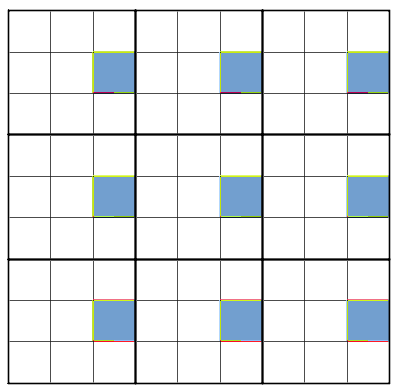
\includegraphics[width=1.4in]{quiz-sample-06/sudoku.png}}
\caption{\label{fig:sudoku} Sudoku board.}
\end{figure}




\vspace{6pt}
{\bf Question 2: Long set operations.} Denote $A_1 = \{ 1 \}$, $A_2 = \{ 1,2 \}$, etc. 
In general, $A_k = \{ 1,2,\ldots,k\}$.\\ 
By $A \oplus B = (A - B) \cup (B-A)$
we denote the symmetric difference: All elements that belong to just one of the
sets $A,B$ (but not the other one). 
Consider this set:
$$S = \bigoplus\limits_{j=1}^{100} A_j = A_1 \oplus A_2 \oplus \ldots \oplus A_{100}.$$
Write a comma-separated list of the $10$ smallest elements of $S$ in 
increasing order.

\vspace{6pt}
{\bf Question 3: Using recurrent formula.}
Find the first $5$ members of this sequence: 
$$\left\{ \begin{array}{l} 
f(0) = 1,\\
f(1) = 4,\\
f(n) = f(n - 1) \cdot f(n - 2) + 1,\; \forall n \geq 2.
\end{array} \right.$$

Write comma-separated values $f(0),f(1),f(2),f(3),f(4)$.

\vspace{6pt}
{\bf Question 4: Reccurent sequence.} A sequence of real numbers 
$f\,:\,\mathbb{N} \rightarrow \mathbb{R}$ satisfies 
the following properties:\\
{\bf (A)} $f(k+2) = f(k) + f(k+1)$ for all integers $k \geq 2$.\\
{\bf (B)} $f(n)$ is a growing geometric progression: Namely $f(1) = f(0) \cdot q$, 
$f(2) = f(0) \cdot q^2$ and so on.


Find the quotient of this geometric progression. Round it to 
the nearest thousandth (i.e. specify the first three digits after the decimal point). 

\vspace{6pt}
{\bf Question 5: Finding a limit.} Define the following sequence: 
$$\left\{ \begin{array}{l} 
x_0 = 1,\\
x_{n+1} = \frac{1}{2} \left( x_n + \frac{2}{x_n}\right),\;\text{if}\;n\geq 0\\
\end{array} \right.$$
Assume that there exists limit $L = \lim_{n \rightarrow \infty} x_n$.\\
Find that limit $L$ and round it to 
the nearest thousandth. 

\vspace{6pt}
{\bf Question 6: Find recurrent formulas.} 
We define three sequences $(a_n)_{n \in \mathbb{N}}$, 
$(b_n)_{n \in \mathbb{N}}$, $(c_n)_{n \in \mathbb{N}}$ explicitly. 
Find their recurrent formulas that allow to find next members of the 
sequence in terms of the previous ones.
\begin{itemize}
\item ${\displaystyle a_n = 2^{\frac{1}{2^n}}}$, where $n \geq 0$. 
\item $b_0 = 1$, $b_1 = 111$, $b_2 = 11111$, $b_3 = 1111111$, etc. 
(In general, the $k$th member $b_k$ has $2k+1$ digits ``1'' in its decimal notation). 
\item $c_n = n^2 + n$, where $n \geq 0$. 
\end{itemize}

\begin{tabular}{|l|l|} \hline
{\bf Initial member} & {\bf Recurrent expression} \\ \hline
$a_0 = \ldots$ & $a_{n+1} = \ldots$ (express via $a_n$ etc.) \\ \hline
$b_0 = \ldots$ & $b_{n+1} = \ldots$ \\ \hline 
$c_0 = \ldots$ & $c_{n+1} = \ldots$ \\ \hline 
\end{tabular}

\vspace{6pt}
{\bf Question 7: Taylor series} There is a formula known from calculus (practically 
used to compute $y = \sin x$) for each $x \in \mathbb{R}$. 
$$\sin x = \sum\limits_{n=0}^{\infty} \frac{(-1)^n \cdot x^{2n+1}}{(2n+1)!} = x - \frac{x^3}{3!}
+ \frac{x^5}{5!} - \ldots$$

Use Python or Scala to add the first $20$ terms of this infinite sum
to compute $\sin 30^{\circ}$. Round the answer
to the nearest thousandth.
(Taylor series expects to have argument $x$ in radians, so you have to convert degrees to radians 
before using the formula.)





\newpage

\subsection{Answers}

\vspace{6pt}
{\bf Question 1.} Answers:\\ 
{\bf (A1)} $80 = 3 \cdot 3 \cdot 9 - 1$ conjunctions.\\
{\bf (A2)} $648 = 81 \cdot 8$ disjunctions,\\
{\bf (A3)} $3 \cdot 3 \cdot 9 \cdot 3 \cdot 3 = 729$ instances of predicate $p$.\\
{\bf (B)} $\bigwedge\limits_{i = 1}^{3} \bigwedge\limits_{j = 1}^{3} \bigwedge\limits_{n = 1}^{9}
\bigvee\limits_{r = 0}^{2} \bigvee\limits_{s = 0}^{2} p(3r+i, 3s+j, n).$

\vspace{6pt}
{\bf (A1)} To count conjunctions, expand
the outer three big conjunctions in this expression:
$$\bigwedge\limits_{r = 0}^{2} \bigwedge\limits_{s = 0}^{2} \bigwedge\limits_{n = 1}^{9}
\bigvee\limits_{i = 1}^{3} \bigvee\limits_{j = 1}^{3} p(3r+i, 3s+j, n).$$
At the first step we expand the outermost $\bigwedge\limits_{r=0}^2$ 
would get three similar subexpressions:
$$\left( \mbox{let $r=0$ in}\; 
\bigwedge\limits_{s = 0}^{2} \bigwedge\limits_{n = 1}^{9}
\bigvee\limits_{i = 1}^{3} \bigvee\limits_{j = 1}^{3} p(3r+i, 3s+j, n) \right) \bigwedge$$
$$\left( \vphantom{\bigwedge\limits_{s = 0}^{2}} \mbox{let $r=1$ in}\; \ldots \right) \bigwedge 
\left( \vphantom{\bigwedge\limits_{s = 0}^{2}} \mbox{let $r=2$ in}\; \ldots \right).$$
Then we expand the next large conjunction for $s=0,1,2$. We would get $3$ smaller terms
inside every big parentheses:
{\small
$$\Big( (\ldots) \wedge (\ldots) \wedge (\ldots) \Big) \wedge
\Big( (\ldots) \wedge (\ldots) \wedge (\ldots) \Big) \wedge
\Big( (\ldots) \wedge (\ldots) \wedge (\ldots) \Big).$$
}
So far we have $8$ conjunctions: $2$ of them are between the big parentheses, 
and $3 \cdot 2 = 6$ more conjunctions separate the smaller expressions $(\ldots)$. 
After that we are ready to expand each smaller $(\ldots)$ into a conjunction of $9$ terms
for $n=1,2,\ldots,9$. 

In all we have $3 \cdot 3 \cdot 9 = 81$ expressions to separate with conjunction 
symbols ($\wedge$); we need $81-1 = 80$ such separators. 

{\bf (A2)} The number of disjunctions can be calculated in a similar manner: we have $81$ subexpressions
$\bigvee\limits_{i = 1}^{3} \bigvee\limits_{j = 1}^{3} p(3r+i, 3s+j, n)$ for all different 
combinations of $(r,s,n)$. Each subexpression has $8$ disjunctions. 

{\bf (A3)} The number of predicate instances can be counted by multiplying the 
number of elements in all five loops: $3 \cdot 3 \cdot 9 \cdot 3 \cdot 3$. 

{\bf (B)} Let us express that all the cells in the upper right corners
of all nine $3 \times 3$ blocks contain different numbers. 
One of such cells is $(i,j) = (1,1)$ (all the others can be obtained by 
adding $3$ or $6$ to $i$ and/or $j$ - thus we get nine values
$(1,1)$,$(1,4)$,$(1,7)$,
$(4,1)$,$(4,4)$,$(4,7)$,$(7,1)$,$(7,4)$,$(7,7)$). Let us express the 
statement that all the numbers $n=1,\ldots,9$ 
should appear in the shaded cells (see Figure~\ref{fig:sudoku2}):


\begin{figure}[!htb]
\center{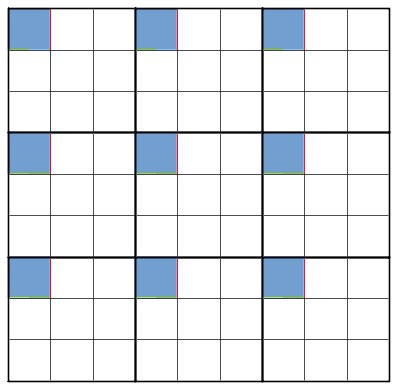
\includegraphics[width=1.4in]{quiz-sample-06/sudoku2.png}}
\caption{\label{fig:sudoku2} Sudoku board.}
\end{figure}

{\small
$$\mbox{let $i=1$,$j=1$ in}\;\forall n\in \{1,\ldots,9 \}:\;\;
\bigvee\limits_{r = 0}^{2} \bigvee\limits_{s = 0}^{2} p(3r+i, 3s+j, n).$$
}

If we want this to be true for any pair $(i,j)$, where both $i$ and $j$ take
all values $1,2,3$:
$$\bigwedge\limits_{i = 1}^{3} \bigwedge\limits_{j = 1}^{3} \bigwedge\limits_{n = 1}^{9}
\bigvee\limits_{r = 0}^{2} \bigvee\limits_{s = 0}^{2} p(3r+i, 3s+j, n).$$

\vspace{6pt}
{\bf Question 2.}\\ Answer: {\tt 2,4,6,8,10,12,14,16,18,20}\\

\begin{figure}[!htb]
\center{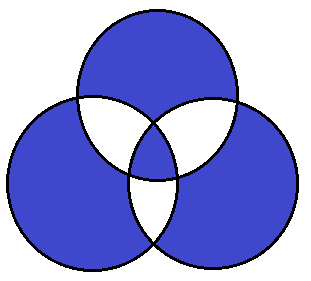
\includegraphics[width=1.4in]{quiz-sample-06/symmetric-differences.png}}
\caption{\label{fig:symmetric-differences} Symmetric differences, 3 sets.}
\end{figure}

Notice that any symmetric difference of two or more sets (Figure~\ref{fig:symmetric-differences})
includes only those elements that belong to an odd number of sets. 
For example, $A_1 \oplus A_2 \oplus A_3$ consists of the elements
that belong to exactly one set ($A_1$, $A_2$ or $A_3$), or 
all three sets: $A_1 \cap A_2 \cap A_3$. 
If you do not believe this, it can be proven by induction. 

Therefore the set $S = \bigoplus\limits_{j=1}^{100} A_j$ contains just those
elements that belong to an odd number of $A_j$. Number $1$ belongs to all $100$ sets
(therefore $1 \not\in S$). But number $2$ belongs to $99$ sets $A_j$ 
(and therefore $2 \in S$). Similarly $4 \in S$, $6 \in S$, and so on. 




\vspace{6pt}
{\bf Question 3:} Answer: {\tt 1,4,5,21,106}\\
We can verify that $f(2) = f(0)\cdot f(1) + 1 = 5$ and so on.

\vspace{6pt}
{\bf Question 4:} Answer: {\tt 1.618}\\
On one hand $f(k+2) = f(k) + f(k+1)$. On the other hand, 
$f(k) = f(0)\cdot q^k$ etc. If we plug into the above formula, we should get:
\begin{equation}
\label{some}
f(0) \cdot q^{k+2} = f(0) \cdot q^k + f(0) \cdot q^{k+1}.
\end{equation}
Since $f(k)$ is strictly increasing, we must have $f(0) \neq 0$ and 
$q > 0$. Namely, the first member in the geometric progression is nonzero, 
and the quotient is positive. 

Therefore the equation (\ref{some}) can be simplified by dividing both sides
with $f(0) \cdot q^k$:
$$q^2 = 1 + q.$$
This quadratic equation has two roots: 
$$q_{1,2} = \frac{1 \pm \sqrt{5}}{2}.$$
Only one of these roots is positive. It is approximately equal to $1.618$. 

{\em Note.} This quotient $q \approx 1.618$ is called {\em golden ratio}. 
For the regular Fibonacci numbers the ratio $F_{n+1}/F_{n}$ approaches 
this number in the limit when $n \rightarrow \infty$.


\vspace{6pt}
{\bf Question 5:} Answer: {\tt 1.414}

Since we know that the sequence 
$x_{n+1} = \frac{1}{2} \left( x_n + \frac{2}{x_n}\right)$ has a limit, then 
both $x_{n+1}$ and $x_n$ go to the same limit as $n$ grows. We have this identity:
$$L = \frac{1}{2} \left (L + \frac{2}{L} \right)$$
and therefore $L^2 =2$ and $L = \pm \sqrt{2}$. Since we start with a positive member, 
all subsequent members will be positive and $L = \sqrt{2}$.

{\em Note.} This recurrence is used in practice to calculate 
square-roots. It converges very fast. Here are the first few members with $15$ decimal digits. 
After six steps we have square root with more than $15$-digit precision.
\begin{verbatim}
x(0) = 1/1 = 1.000000000000000
x(1) = 3/2 = 1.500000000000000
x(2) = 17/12 = 1.416666666666667
x(3) = 577/408 = 1.414215686274510
x(4) = 1.414213562374690
x(5) = 1.414213562373095
x(6) = 1.414213562373095
\end{verbatim}



\vspace{6pt}
{\bf Question 6:} Answers:\\
\begin{tabular}{|l|l|} \hline
{\bf Initial member} & {\bf Recurrent expression} \\ \hline
$a_0 = 2$ & $a_{n+1} = \sqrt{a_n}$ \\ \hline
$b_0 = 1$ & $b_{n+1} = 100\cdot b_n + 11$ \\ \hline 
$c_0 = 0$ & $c_{n+1} = c_n + 2\cdot(n+1)$ \\ \hline 
\end{tabular}

{\bf (A)} Notice that the power in $a_n$ decreases twice with each step. 
So it is equivalent to taking a square-root.\\
{\bf (B)} Decimal representation of $b_{n+1}$ is easy to obtain from $b_n$: 
We first shift all the digits two places to the left (multiply by $100$), then 
add $11$ to get the last two digits equal to "11".\\
{\bf (C)} Compute the first few members of the sequence $c_n$: 
$0$, $2$, $6$, $12$, $20$. Their differences make an arithmetic progression: 
$2-0 = 2$, $6-2 = 4$, $12-6=6$, etc. So it is possible to compute the next
member by adding $2(n+1)$ (the $n$th even number).



\vspace{6pt}
{\bf Question 7:}

 


\end{document}



\newpage
\documentclass[jou]{apa6}

\usepackage[american]{babel}

\usepackage{csquotes}
\usepackage[style=apa,sortcites=true,sorting=nyt,backend=biber]{biblatex}
\DeclareLanguageMapping{american}{american-apa}
\addbibresource{bibliography.bib}


%%%%%%%%%%%%%%%%%%%%%%%%%%%%%%%%%%%%%%%%
%% Discrete Structures
%% The start of RBS stuff
%%%%%%%%%%%%%%%%%%%%%%%%%%%%%%%%%%%%%%%%

% Working internal and external links in PDF
\usepackage{hyperref}
% Extra math symbols in LaTeX
\usepackage{amsmath}
\usepackage{gensymb}
\usepackage{amssymb}
% Enumerations with (a), (b), etc.
\usepackage{enumerate}

\let\OLDitemize\itemize
\renewcommand\itemize{\OLDitemize\addtolength{\itemsep}{-6pt}}

\usepackage{etoolbox}
\makeatletter
\preto{\@verbatim}{\topsep=3pt \partopsep=3pt }
\makeatother

% These sizes redefine APA for A4 paper size
\oddsidemargin 0.0in
\evensidemargin 0.0in
\textwidth 6.27in
\headheight 1.0in
\topmargin -24pt
\headheight 12pt
\headsep 12pt
\textheight 9.19in

\setlength\parindent{0pt}

\title{Sample Quiz 4}
\author{Discrete Structures, Spring 2020}
\affiliation{RBS}

\leftheader{Discrete Quiz 6}

\abstract{%
}

%\keywords{}

\begin{document}

%\thispagestyle{empty}

\twocolumn
\section{Quiz 6: Recurrent Sequences}

\vspace{10pt}
{\bf Question 1: Modifying Sudoku Rules.}\\ 
We have a $9 \times 9$ table; each cell contains one number from 
$A_9 = \{ 1, 2,\ldots, 9 \}$. 
Number $a_{i,j}$ describes the number written on Line $i$ and
Column $j$ in the table (and $i,j \in A_9$). 

Identify the formula describing that the sum of all numbers in one 
diagonal of the table $9 \times 9$ is equal to the sum of all numbers
on the other diagonal of the table.

{\bf (A)} ${\displaystyle \sum\limits_{r=0}^{8} a_{r+1,r+1} = \sum\limits_{r=0}^{8} a_{9-r,r+1}}$\\
{\bf (B)} ${\displaystyle \sum\limits_{r=0}^{8} a_{r,r} = \sum\limits_{r=0}^{8} a_{9-r,r}}$\\
{\bf (C)} ${\displaystyle \sum\limits_{r=0}^{8} a_{r+1,r+1} = \sum\limits_{r=0}^{8} a_{10-r,r+1}}$\\
{\bf (D)} ${\displaystyle \sum\limits_{r=0}^{8} a_{r,r} = \sum\limits_{r=0}^{8} a_{10-r,r}}$

\vspace{6pt}
{\bf Question 2: Computing sums.}\\ 
Find the values of these sum in a Sudoku table (it is known that each number from $A_9 = \{ 1, 2,\ldots, 9 \}$ 
is written exactly once in all rows, in all columns and also in all $3 \times 3$ blocks). 


$${\displaystyle \sum\limits_{r=1}^{9} \sum\limits_{s=1}^{9} a_{r,s}}$$

Write in the number as your answer.




\vspace{6pt}
{\bf Question 3: Long set operations.} Denote $A_1 = \{ 1 \}$, $A_2 = \{ 1,2 \}$, etc. 
In general, $A_k = \{ 1,2,\ldots,k\}$.\\ 
By $A \oplus B = (A - B) \cup (B-A)$
we denote the symmetric difference: All elements that belong to just one of the
sets $A,B$ (but not the other one). 
Consider this set:
$$S = \bigoplus\limits_{j=1}^{100} A_{2j-1}.$$
Write a comma-separated list of the $10$ smallest elements of $S$ in 
increasing order.


\vspace{6pt}
{\bf Question 4: Using recurrent formula.}
Find the first $6$ members of this infinite sequence ($C_0,C_1,C_2,\ldots$): 
$$\left\{ \begin{array}{l} 
C_0 = 1,\\
C_{n+1} = \sum\limits_{i=0}^n (C_i \cdot C_{n-i}).
\end{array} \right.$$

In your answer write comma-separated values:\\
$C_0,C_1,C_2,C_3,C_4,C_5$.



\vspace{6pt}
{\bf Question 5: Reccurent sequence.} A sequence of real numbers 
$f\,:\,\mathbb{N} \rightarrow \mathbb{R}$ satisfies 
the following properties:\\
{\bf (A)} $f(k+2) = 2f(k+1) + f(k)$ for all integers $k \geq 2$.\\
{\bf (B)} $f(n)$ is a geometric progression.

Find some quotient of this geometric progression (if there are several possibilities, pick any of them). 
Round it to the nearest thousandth, i.e. specify the first three digits after the decimal point). 


\vspace{6pt}
{\bf Question 6: Finding a limit.} Define the following sequence: 
$$\left\{ \begin{array}{l} 
x_0 = 1,\\
x_{n+1} = \frac{1}{3} \left( 2x_n + \frac{7}{x_n^2}\right),\;\text{if}\;n\geq 0\\
\end{array} \right.$$
Assume that there exists limit $L = \lim_{n \rightarrow \infty} x_n$.\\
Find that limit $L$ and round it to 
the nearest thousandth. 



\vspace{6pt}
{\bf Question 7: Taylor series} There is a formula known from calculus (practically 
used to compute $y = \sin x$) for each $x \in \mathbb{R}$. 
$$\sin x = \sum\limits_{n=0}^{\infty} \frac{(-1)^n \cdot x^{2n+1}}{(2n+1)!} = x - \frac{x^3}{3!}
+ \frac{x^5}{5!} - \ldots$$

Use Python or Scala to add the first $20$ terms of this infinite sum
to compute $\sin 1080^{\circ}$. Round the answer
to $15$ digits (this usually happens by itself: double precision numbers are output in this manner).





\newpage

\subsection{Answers}


\vspace{6pt}
{\bf Question 1.} Answer: {\tt A}\\
All other variants refer to $a_{ij}$, where $i$ or $j$ are outside the interval $[1;9]$, 
so they are not defined. Answer (A), on the other hand, refers to the elements that
lay on both diagonals.

\vspace{6pt}
{\bf Question 2.} Answer: {\tt 405}\\
This summation is the total of all elements in the Sudoku table. 
Each row contains all numbers from $1$ to $9$. So they add up to 
$45 = \frac{9 \cdot (9+1)}{2}$. This has to be multiplied by $9$, since
there are $9$ rows. 

\vspace{6pt}
{\bf Question 3.} Answer:\\ {\tt 2,3,6,7,10,11,14,15,18,19}\\
The smallest number $1 \not\in S$, because it belongs to all $100$ sets (so it cancels out, when 
we compute the long symmetric sum).\\
Numbers $2$ and $3$ belong to exactly $99$ sets, therefore they are included.\\
Numbers $4$ and $5$ belong to exactly $98$ sets, so they are not included, and so on. 



\vspace{6pt}
{\bf Question 4.} Answer: {\tt 1,1,2,5,14,42}\\
We can simply plug into the formulas: 
$$\left\{ \begin{array}{l}
C_1 = C_0 \cdot C_0 = 1 \cdot 1 = 1\\
C_2 = C_0 \cdot C_1 + C_1 \cdot C_0 = 1 \cdot 1 + 1 \cdot 1 = 2\\
C_3 = C_0 \cdot C_2 + C_1 \cdot C_1 + C_2 \cdot C_0 = 5\\
\ldots
\end{array} \right.$$

These are also known as {\em Catalan numbers}. 
For example $C_3$ shows, in how many ``essentially different'' ways you can put parentheses
in an expression with four letters and three binary operators:
$$(((a \circ b) \circ c) \circ d);\; ((a \circ (b \circ c)) \circ d);$$
$$((a \circ b) \circ (c \circ d));\; (a \circ ((b \circ c) \circ d));$$ 
$$(a \circ (b \circ (c \circ d)))$$

Here we assume that the $\circ$ operation is neither associative nor commutative. 
Certainly, we could insert even more parentheses; but these $5$ ways differ 
by the order of execution of these three operations.



\vspace{6pt}
{\bf Question 5.} Answer: {\tt 2.414} {\bf or} {\tt -0.414}\\
If we substitute the geometric progression $f(n) = f(0) \cdot q^n$ 
into the equation $f(k+2) = 2f(k+1) + f(k)$: 
$$f(0) \cdot q^{k+2} = 2f(0) \cdot q^{k+1} + f(0) \cdot q^{k}.$$

Now there are three possibilities.\\
{\bf Case 1.} If $f(0) = 0$, then the sequence 
$0,0,\ldots$ is a (degenerated) version of a geometric series. 
Any number can be its quotient; so it is not interesting to solve this.\\
{\bf Case 2.} If $f(0) \neq 0$, we could still take $q = 0$, but this
is also a degenerated geometric series of all zeroes (except the first member $f(0)$).
This is not interesting either.\\
{\bf Case 3.} If $f(0)$ and $q$ are both nonzero, we can cancel them in the
above equation and get this: $q^2 = 2q + 1$. 
The two roots are 
$$q_{1,2} = \frac{2 \pm \sqrt{4 + 4}}{2} = 1 \pm \sqrt{2}.$$
Either answer $1 - \sqrt{2}$ or $1 + \sqrt{2}$ is valid. 




\vspace{6pt}
{\bf Question 6.} If the limit $L$ exists, then both $x_n$ and $x_{n+1}$ both 
go to that limit, and we must have the identity:
$$L = \frac{1}{3}\left( 2L + \frac{7}{L^2} \right).$$
When we express $L$ from that equation, we get $L = \sqrt[3]{7}$. 

In fact, the sequence does converge to the cubic root: 
\begin{verbatim}
x(0) = 1.000000000000000
x(1) = 3.000000000000000
x(2) = 2.259259259259259
x(3) = 1.963308018221572
x(4) = 1.914212754165601
x(5) = 1.912932040596942
x(6) = 1.912931182772774
x(7) = 1.912931182772389
x(8) = 1.912931182772389
\end{verbatim}


\vspace{6pt}
{\bf Question 7.} Answer:\\ {\tt -482.8813747415584} (or similar)

In theory $\sin 1080^{\circ} = 0$ (and Taylor series should converge to $0$), 
but this nonsense result happens because of huge rounding errors.

{\footnotesize
\begin{verbatim}
object TaylorSeries {

  def factorial(n:Int):Double = {
    n match {
      case 0 => 1.0
      case n => n*factorial(n-1)
    }
  }
    
  def sin(x:Double,nTerms:Int):Double = {
    val terms = 
      for (k <- List.range(0,nTerms)) 
        yield { math.pow(-1,k)*
        math.pow(x,2*k+1)/factorial(2*k+1) } 
    terms.foldLeft(0.0)((a,b) => a+b)
  }
  
  def main(args:Array[String]): Unit = {
    val nTerms = 20
    val x = Math.PI*6 // (1080/180)*PI = 6PI 
    println(sin(x,nTerms))
  }
}
\end{verbatim}
}



\end{document}




\newpage
\documentclass[jou]{apa6}

\usepackage[american]{babel}

\usepackage{csquotes}
\usepackage[style=apa,sortcites=true,sorting=nyt,backend=biber]{biblatex}
\DeclareLanguageMapping{american}{american-apa}
\addbibresource{bibliography.bib}


%%%%%%%%%%%%%%%%%%%%%%%%%%%%%%%%%%%%%%%%
%% Discrete Structures
%% The start of RBS stuff
%%%%%%%%%%%%%%%%%%%%%%%%%%%%%%%%%%%%%%%%

% Working internal and external links in PDF
\usepackage{hyperref}
% Extra math symbols in LaTeX
\usepackage{amsmath}
\usepackage{gensymb}
\usepackage{amssymb}
% Enumerations with (a), (b), etc.
\usepackage{enumerate}

\let\OLDitemize\itemize
\renewcommand\itemize{\OLDitemize\addtolength{\itemsep}{-6pt}}

\usepackage{etoolbox}
\makeatletter
\preto{\@verbatim}{\topsep=3pt \partopsep=3pt }
\makeatother

% These sizes redefine APA for A4 paper size
\oddsidemargin 0.0in
\evensidemargin 0.0in
\textwidth 6.27in
\headheight 1.0in
\topmargin -24pt
\headheight 12pt
\headsep 12pt
\textheight 9.19in



\title{Sample Quiz 4}
\author{Discrete Structures, Spring 2020}
\affiliation{RBS}

\leftheader{Discrete Sample Quiz 7}

\abstract{%
}

%\keywords{}

\setlength\parindent{0pt}

\begin{document}

%\thispagestyle{empty}

\twocolumn
\section{Worksheet 7: Counting}

\vspace{10pt}
{\bf Question 1 (Traversing Rubik's Cube).} A tiny ant wants to travel 
between two opposite vertices of a $3 \times 3 \times 3$ cube. It can crawl
on the surface of the cube (and even inside it); but any path should consist from exactly $9$ unit-length
steps, where each step is parallel to one of the coordinate axes ($x$, $y$ or $z$). 
Find the number of paths that the ant could take as it crawls from the vertex $A$ to the vertex $B$. 
\begin{center}
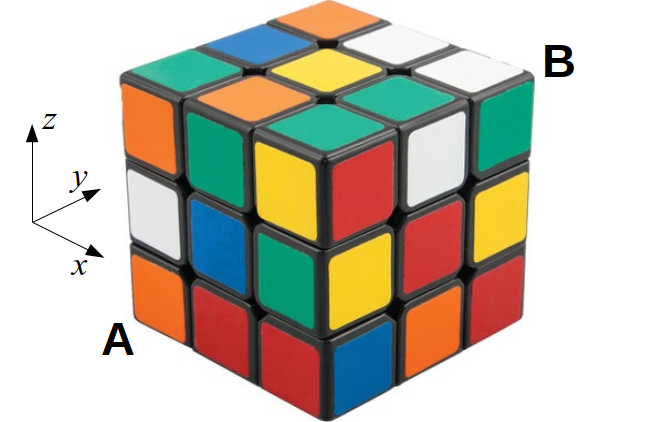
\includegraphics[width=2in]{rubiks-cube.png}
\end{center}

Write your answer as an integer number equal to the number of paths from $A$ to $B$ satisfying the condition.






\vspace{6pt}
{\bf Question 2 (Permutations with Repetition).}\\
{\bf (A)} Find the number of ways (denoted by $N$) one can arrange the letters in the 6-letter word {\tt OLIVIA}. 
Both letters "I" are not distinguishable (if they switch places, it is still the same arrangement).\\
{\bf (B)} Assume that somebody writes out all the permutations of the word {\tt OLIVIA} 
in the {\em lexicographic ordering} (ordered as in a dictionary: sorted by the 1st letter; 
if the 1st letter is the same, then by the 2nd letter, etc.).\\
For example, the first permutation: $w_1 = \mathtt{AIILOV}$ and the last one is $w_N = \mathtt{VOLIIA}$. 
Find the permutations $w_{60},w_{61},w_{62},w_{63}$. 

Write your answer as a comma-separated list (first the total number of permutations, then the
$60$th,$61$st,$62$nd,$63$rd permutation).\\
$N$,$w_{60},w_{61},w_{62},w_{63}$. 


\vspace{6pt}
{\bf Question 3 (Raising to a high power).} 
Joe wrote the decimal notation of the following number:
$$X = \left( 10^{10} + 1 \right)^{10}.$$
After that, Joe erased the last $50$ digits of the number $X$, and got the number $Y$. 
Finally, Joe erased all the digits of $Y$, except the last ten digits, and got a sequence of digits $Z$.\\
{\bf (A)} Write all the digits of $Z$ (if it has leading zeroes, write them as well).\\
{\bf (B)} Express $Z$ as $C_n^k$ (``$n$ choose $k$''), where $k \leq n$.

Write your answer like this:\\ {\tt dddddddddd,choose(n,k)}.


\vspace{6pt}
{\bf Question 4 (Combinations with Repetition).} You have unlimited number of jellybeans \textendash{}
they can have any of these four colors: red, orange, green, yellow. The jellybeans of each
color are identical. Solve the following: express your answers as a binomial coefficients "$n$ choose $k$", 
where $k \leq n$.

{\bf (A)}  How many collections of $20$ jellybeans can you make? (The order of jellybeans in the collection 
does not matter. Those jellybean collections that have the same number of each color are considered identical.)\\
{\bf (B)} How many collections of $20$ jellybeans can you make, if there has to be at least one jellybean 
of each color. 

Write your answer in a form:\\ {\tt choose(n1,k1),choose(n2,k2)}\\
Replace {\tt n1,k1,n2,k2} with appropriate integers.


\vspace{6pt}
{\bf Question 5 (Ordering your combinations).} 
Somebody has written out all the combinations, how to choose $k=4$ months out of a set of 
$n=12$ months:\\
{\small
$\{ \mathtt{JAN},\mathtt{FEB},\mathtt{MAR},\mathtt{APR},\mathtt{MAY},\mathtt{JUN},
\mathtt{JUL},\mathtt{AUG},\mathtt{SEP},\mathtt{OCT},\mathtt{NOV},\mathtt{DEC} \}.$
}

All these four-month combinations are written in a sorted (so that a month appearing earlier in a year is always
written first), and furthermore \textendash{} all these combinations are arranged in increasing order. 
Months are ordered in this way: $\mathtt{JAN} < \mathtt{FEB} < \ldots < \mathtt{DEC}$.\\
The very first combination of months is $\mathtt{JAN},\mathtt{FEB},\mathtt{MAR},\mathtt{APR}$, 
the last one is $\mathtt{SEP},\mathtt{OCT},\mathtt{NOV},\mathtt{DEC}$. 

Write a comma-separated list of the four-months that is in the $100$th place in this list. 


\vspace{6pt}
{\bf Question 6: Pennies and jars.} 
Assume that you have $50$ pennies and three jars (these jars are initially labeled $A$, $B$, and $C$). 

{\bf (A)} In how many ways can you put the pennies in the jars, assuming that the pennies and the jars are distinguishable?\\
{\bf (B)} In how many ways can you put the pennies in the jars, assuming that the pennies are identical, but jars are distinguishable?\\
{\bf (C)} Assume that we remove the labels ($A$,$B$,$C$) from the jars; and the jars become indistinguishable. 
In how many ways can you put the pennies in the jars, assuming that both the pennies and the jars are indistinguishable?

\vspace{6pt}
{\bf Question 7 (Necklace with colored beads).} Assume that we have a circular necklace with 
$2012$ equally spaced beads. Exactly $7$ of the beads are red, the remaining ones are white. 
How many necklaces there are? (Necklaces that is obtainable from each other by rotating the
circle by some angle $\frac{2\pi}{2012}k$ ($k = 1,\ldots,2011$) are considered identical.)

{\em Note.} A more general question was asked in CGMO (China Girls Mathematical Olympiad), 
see Problem 8, \url{https://bit.ly/2TcfHH5}. 


\newpage
\subsection{Answers}

\vspace{6pt}
{\bf Question 1} Answer: {\tt 1680}\\
Every unit move of the ant can be expressed by a letter $X,Y,Z$ (depending 
on its direction). There are altogether $9!$ ways to arrange 
nine letters. Since all three letters $X$ can be mixed in any order, we need
to divide by $3! = 6$. For the same reason we can also mix all three $Y$s and 
all three $Z$s. Ultimately, 

$$\frac{9!}{3!3!3!} = 1680.$$

\vspace{6pt}
{\bf Question 2} Answer: TBD\\

\vspace{6pt}
{\bf Question 3} Answer: TBD\\

\vspace{6pt}
{\bf Question 4} Answer: TBD\\

\vspace{6pt}
{\bf Question 5} Answer: TBD\\

\vspace{6pt}
{\bf Question 6} Answer: TBD\\

\vspace{6pt}
{\bf Question 7} Answer: TBD\\






\end{document}



\newpage
\documentclass[jou]{apa6}

\usepackage[american]{babel}

\usepackage{csquotes}
\usepackage[style=apa,sortcites=true,sorting=nyt,backend=biber]{biblatex}
\DeclareLanguageMapping{american}{american-apa}
\addbibresource{bibliography.bib}


%%%%%%%%%%%%%%%%%%%%%%%%%%%%%%%%%%%%%%%%
%% Discrete Structures
%% The start of RBS stuff
%%%%%%%%%%%%%%%%%%%%%%%%%%%%%%%%%%%%%%%%

% Working internal and external links in PDF
\usepackage{hyperref}
% Extra math symbols in LaTeX
\usepackage{amsmath}
\usepackage{gensymb}
\usepackage{amssymb}
% Enumerations with (a), (b), etc.
\usepackage{enumerate}
\usepackage{xcolor}

\let\OLDitemize\itemize
\renewcommand\itemize{\OLDitemize\addtolength{\itemsep}{-6pt}}

\usepackage{etoolbox}
\makeatletter
\preto{\@verbatim}{\topsep=3pt \partopsep=3pt }
\makeatother

% These sizes redefine APA for A4 paper size
\oddsidemargin 0.0in
\evensidemargin 0.0in
\textwidth 6.27in
\headheight 1.0in
\topmargin -24pt
\headheight 12pt
\headsep 12pt
\textheight 9.19in



\title{Sample Quiz 4}
\author{Discrete Structures, Spring 2020}
\affiliation{RBS}

\leftheader{Discrete Quiz 7}

\abstract{%
}

%\keywords{}

\setlength\parindent{0pt}

\begin{document}

%\thispagestyle{empty}

\twocolumn
\section{Quiz 7: Counting}

% P1: 4+4 

\vspace{10pt}
{\bf Question 1 (Placing 8 rooks).} Somebody has an $8 \times 8$ chessboard and 
$8$ rooks ($4$ of them black, $4$ of them white). 
In how many ways one can place these $8$ rooks on the chessboard so that 
no rook shares the same horizontal or vertical with any other rook. 
Assume that the rooks of the same color are not distinguishable (but the chessboard itself cannot be rotated 
or flipped - i.e.\ we count symmetric positions multiple times).
\begin{center}

\includegraphics[width=2in]{quiz7/chessboard.png}
\end{center}

Write your answer as an integer number. 



\vspace{6pt}
{\bf Question 2 (Finding a higher order derivative).}\\
There is a formula to compute the 1st derivative of a product: 
$$(uv)' = u'v + v'u.$$
Assume that you need to compute the 4th derivative of a product of two functions $u\cdot v$. 
Enter the formula to compute $(uv)''''$. 

Your answer can use letters $u$, $v$, 
apostrophes (denoting the derivatives of the 1st, 2nd, 3rd and 4th degree), 
asterisk {\tt *} denoting multiplication and integer numbers. 


\vspace{6pt}
{\bf Question 3 (Multinomial formula).}\\
As a generalization to the Newton's binomial theorem (the expression for $(a+b)^n$), there
is also a more general {\em multinomial theorem}: 
$$(x_1 + x_2  + \cdots + x_m)^n
 = \sum\limits_{k_1+k_2+\cdots+k_m=n} {n \choose k_1, k_2, \ldots, k_m}
  \prod_{t=1}^m x_t^{k_t}\,,$$
where the {\em multinomial coefficients} are computed like this:
$${n \choose k_1, k_2, \ldots, k_m}
 = \frac{n!}{k_1!\, k_2! \cdots k_m!}$$

Assume that you use the multinomial formula to open parentheses in the following expression $(a+b+c)^9$.\\
{\bf (A)} How many {\em terms} are added in this expression?  (A term is a product 
of some number with the powers: $k\cdot a^x b^y c^z$, where $k$ is a positive number, but 
$x,y,z$ are nonnegative integers.)\\
{\bf (B)} What is the coefficient for the term $a^3b^3c^3$ in this expansion?

Write two numbers separated by a comma.




\vspace{6pt}
{\bf Question 4 (Permutations of ANNA).} Create a list of all permutations
of the letters in the word {\tt ANNA}. Assume that both copies of "A" and "N" are indistinguishable. 

Write an alphabetically sorted list separated by commas.


\vspace{6pt}
{\bf Question 5 (Pennies in jars).} 
Somebody has 5 pennies and 4 jars. All pennies are distinguishable and each penny should go into some jar. 
All the jars are placed in the vertices of a square $ABCD$; jar locations that differ only by rotations of that
square are considered indistinguishable. (For example, if all the pennies from the vertex $A$ would go to $B$; 
all pennies from $B$ would go to $C$, from $C$ to $D$, and from $D$ to $A$, then it would be the same way to distribute pennies.)

Find the number of ways how the pennies can be distributed among these jars. Write your answer as an integer.



\vspace{6pt}
{\bf Question 6 (Odd binomial coefficients).} Assume the following Kummer's theorem (\url{https://bit.ly/38Bak99}):\\
The binomial coefficient ${n \choose k} = C_n^k = \frac{n!}{k!(n-k)!}$ is odd iff
adding the binary notations of $k$ and $n-k$ there are no carries.\\ 
For example, the binomial coefficients ${10 \choose k}$ where $k=0,\ldots,10$ are the following:
$$\textcolor{red}{1},10,\textcolor{red}{45},120,210,252,210,120,\textcolor{red}{45},10,\textcolor{red}{1}.$$
The only odd numbers are ${10 \choose 0}$, ${10 \choose 2}$, ${10 \choose 8}$, ${10 \choose 10}$, 
since $0_{2} + 1010_{2}$ and also $10_{2} + 1000_{2}$ can be added without any carries (i.e.\
adding these we won't run into situation where we need to add $1+1$ or $1+1+1$ anywhere: Every situation 
where some digit is ``carried over'' from a smaller position of the binary number to a larger one is called a ``carry''.)

Find the number of odd numbers ${2020 \choose k}$, where $k = 0,1,\ldots,2020$. 
Express your answer as an integer number in decimal notation.


\vspace{6pt}
{\bf Question 7 (Sorted permutations).} As we know there are $5! = 120$ ways how to write the 5-letter word
{\tt ABCDE} (using every letter exactly once). Find the word that is written in the 100th position (assuming that
all the 120 permutations are sorted alphabetically).

Write your answer as 5-letter word.



\newpage

\subsection{Answers}

\vspace{4pt}
{\bf Question 1.} Answer: {\tt 2822400}\\
{\bf Statement 1:} If rooks would be the same color (so that the ``individuality'' of a rook 
does not matter), then we could have $8! = 40320$ different placements.\\
On the first horizontal you can place a rook in $8$ different ways (choose any vertical), 
on the second horizontal you can place a rook in $7$ different ways (one vertical is already taken) and so on. 
Finally, you multiply all these numbers together.\\
{\bf Statement 2:} You can pick the four horizontals containing white rooks in ${8 \choose 4} = 70$ different ways.\\
This follows immediately from the definition of a combination of $k=4$ elements out of an $n=8$ element set.

The total can be obtained, if we multiply $8!$ (placements of indistinguishable rooks) by ${8 \choose 4}$. 
The product is $40320 \cdot 70 = 2822400$.

\vspace{10pt}
{\bf Question 2.} Answer:\\
$\mathtt{u''''*v+4*u'''*v'+6*u''*v''+4*u'*v'''+v''''}$\\
{\em (In your responses the multiplication could be omitted, and also the 
order of summation can be different.)}\\
Let us verify, why expanding the expression $(uv)''''$ leads to the same binomial coefficients
as Newton's binom $(a+b)^4$. We express successive derivatives:
\begin{align}
(uv)' & = u'v + uv'. \\
(uv)'' & = (u'v + uv')' = (u'v)' + (uv')' = \nonumber \\
 & = (u''v + u'v') + (u'v' + uv'') = \nonumber \\
 & = u''v + 2u'v' + uv''.\\
(uv)''' & = (u''v + 2u'v' + uv'')' = \nonumber \\
 & = (u''v)' + 2(u'v')' + (uv'')' = \nonumber \\
 & = (u'''v + u''v') + 2(u''v' + u'v'') + (u'v'' + uv''') = \nonumber \\
 & = u'''v + 3u''v' + 3u'v'' + uv'''.\\
(uv)'''' & = (u'''v + 3u''v' + 3u'v'' + uv''')' = \nonumber \\
 & = u''''v+4u'''v'+6u''v''+4u'v'''+v''''.
\end{align}


\vspace{10pt}
{\bf Question 3.} Answer: {\tt 55,1680}\\
To see, how many terms there are in the expansion of $(a+b+c)^9$, 
notice that each term is in form $a^xb^yc^z$, where $x,y,z$ are nonnegative
integers satisfying $x+y+z=9$. To count the ways how $n=9$ can be expressed
as a sum of $k=3$ nonnegative numbers, we compute the {\em combination with 
repetitions}. The formula for combination with repetitions is this:
$${n+k-1 \choose k-1} = {9+3-1 \choose 3-1} = {11 \choose 2} = \frac{11 \cdot 10}{2 \cdot 1} = 55.$$

By multinomial formula, the coefficient for $a^3b^3c^3$ is $\frac{9!}{3!3!3!} = 1680$.



\vspace{10pt}
{\bf Question 4.}\\ Answer: {\tt AANN,ANAN,ANNA,NAAN,NANA,NNAA}\\
The number of permutations with repetitions equals $\frac{4!}{2!}{2!} = \frac{24}{2 \cdot 2} = 6$.
We have four letters (and two of them repeat twice each).
Once we sort all the permutations alphabetically, we get the answer: 
the first three permutations start by ``A'', the next three start by ``N''.

\vspace{10pt}
{\bf Question 5.} Answer: {\tt 256}\\
Each penny can be placed in any of the four jars. We make this choice five times, so the
total number of ways is $4^5 = 1024$. Moreover, you can rotate the four jars in four different ways (getting
essentially identical ways to distribute pennies, which have been counted four times each). 
So the final answer can be obtained by dividing $1024/4 = 256$.

Another solution: Place the first penny in one of the jars.
Since the pennies are all distinguishable, this jar is very special.
Place that jar in the North position, then the remaining jars are facing East, South and West.
And then you can make four choices with four outcomes each. So the result is still $4^4 = 256$.

\vspace{10pt}
{\bf Question 6.} Answer: {\tt 128}\\
We have this equality:
$$2020 = 1024 + 512 + 256 + 128 + 64 + 32 + 4,$$
So $2020_{10} = 11111100100_2$. The binary notation for $2020$
contains digit $1$ in $7$ positions. 

There are altogether
$2^7 = 128$ how you can split these seven digits $1$ between 
$k$ and $2020-k$ so that when you add $k$ and $2020-k$ (in binary notation) 
you do not get any carries. Here are some of these ways:\\
{\small
$\mathtt{11111100100}_2 = \mathtt{11111100100}_2 + \mathtt{0}_2 = 2020_{10}+0_{10}$,\\
$\mathtt{11111100100}_2 = \mathtt{11111100000}_2 + \mathtt{100}_2 = 2016_{10} + 4_{10}$,\\
$\mathtt{11111100100}_2 = \mathtt{11111000100}_2 + \mathtt{100000}_2 = 1988_{10} + 32_{10}$,\\
$\mathtt{11111100100}_2 = \mathtt{11111000000}_2 + \mathtt{100100}_2 = 1984_{10} + 36_{10},\ldots$\\
$\mathtt{11111100100}_2 = + \mathtt{0}_2 + \mathtt{11111100100}_2  = 0_{10} + 2020_{10}$.\\
}
So, all ${2020 \choose 0}$,  ${2020 \choose 4}$,  ${2020 \choose 32}$,  ${2020 \choose 36}$, etc. are odd.



\vspace{10pt}
{\bf Question 7.} Answer: {\tt EACDB}.\\
There are $24$ permutations of {\tt ABCDE} starting with each 
letter (A,B,C,D and E). The first $24+24+24+24=96$ of them start by A,B,C,D respectively. 
So the 100th permutation would start by ``E'', and it will be the 4th out of them. 
We can create a sequence of the (alphabetically) first four permutations starting by ``E'':
$$\mathtt{EABCD},\mathtt{EABDC},\mathtt{EACBD},\mathtt{EACDB},\ldots$$
We see that the 100th permutation (or the 4th among those starting by ``E'') is 
{\tt EACDB}.

\end{document}





\newpage
\documentclass[jou]{apa6}

\usepackage[american]{babel}

\usepackage{csquotes}
\usepackage[style=apa,sortcites=true,sorting=nyt,backend=biber]{biblatex}
\DeclareLanguageMapping{american}{american-apa}
\addbibresource{bibliography.bib}


%%%%%%%%%%%%%%%%%%%%%%%%%%%%%%%%%%%%%%%%
%% Discrete Structures
%% The start of RBS stuff
%%%%%%%%%%%%%%%%%%%%%%%%%%%%%%%%%%%%%%%%

% Working internal and external links in PDF
\usepackage{hyperref}
% Extra math symbols in LaTeX
\usepackage{amsmath}
\usepackage{gensymb}
\usepackage{amssymb}
% Enumerations with (a), (b), etc.
\usepackage{enumerate}

\let\OLDitemize\itemize
\renewcommand\itemize{\OLDitemize\addtolength{\itemsep}{-6pt}}

\usepackage{etoolbox}
\makeatletter
\preto{\@verbatim}{\topsep=3pt \partopsep=3pt }
\makeatother

% These sizes redefine APA for A4 paper size
\oddsidemargin 0.0in
\evensidemargin 0.0in
\textwidth 6.27in
\headheight 1.0in
\topmargin -24pt
\headheight 12pt
\headsep 12pt
\textheight 9.19in



\title{Sample Quiz 8}
\author{Discrete Structures, Spring 2020}
\affiliation{RBS}

\leftheader{Discrete Sample Quiz 8}

\abstract{%
}

%\keywords{}

\setlength\parindent{0pt}

\begin{document}

%\thispagestyle{empty}

\twocolumn
\section{Worksheet 8: Probabilities}

\vspace{10pt}
{\bf Question 1} 
What is the probability that the sum of the numbers on two dice is even when they are rolled?\\
(Express your answer as $P/Q$.)

\vspace{10pt}
{\bf Question 2}\\
{\bf (A)} What is the probability to get sequence ``{\tt Heads}, {\tt Heads}, {\tt Heads}, 
{\tt Heads}, {\tt Heads}, {\tt Heads}'' when 
tossing a coin?\\
{\bf (B)} What is the probability to get sequence ``{\tt Heads, Tails, Heads, Tails, Heads, Tails, Heads, Tails}'' when 
tossing a coin?\\
{\bf (C)} What is the probability to get even number of "Heads" when tossing a coin 6 times?

\vspace{10pt}
{\bf Question 3}
Assume that there is the following gambling game involving dice (cube with six outcomes: $1,2,3,4,5,6$ with 
equal probabilities). Player $A$ guesses a number $n$ between $1$ and $6$ (for example $n = 3$). Then he rolls a dice three times. 
We have the following four outcomes (events):\\
$E_1$: If one of the dice rolls equals Player's $A$ number $n$, then Player $A$ wins 1 euro.\\
$E_2$: If two of the dice rolls equal Player's $A$ number $n$, then Player $A$ wins 2 euros.\\
$E_3$: If all three dice rolls equal Player's $A$ number $n$, then Player $A$ wins 3 euros.\\
$E_4$: If none of the dice rolls equals $n$, then Player $A$ loses 1 euro.\\
{\bf (A)} Find the probability for each event $E_1,E_2,E_3,E_4$.\\
{\bf (B)} Find the expected value of the money that Player $A$ wins or loses during a single round of this game. (One round = three 
dice rolls as described above). Use this formula \textendash{} a weighted sum of the euros multiplied by the respective probabilities:
$$p(E_1)\cdot 1 + p(E_2)\cdot 2 + p(E_3)\cdot 3 + p(E_4)\cdot (-1).$$


\vspace{10pt}
{\bf Question 4} Find a probability that choosing a random month during a leap year, it would have exactly $5$ Sundays.

\vspace{10pt}
{\bf Question 5} Suppose you and a friend each choose at random an integer between $1$ and $8$, inclusive. For example, some
possibilities are $(3,7)$, $(7,3)$, $(4,4)$, $(8,1)$, where your number is written first and your friend’s number second.
Find the following probabilities:\\
{\bf (A)} p(you pick 5 and your friend picks 8).\\
{\bf (B)} p(sum of the two numbers picked is < 4).\\
{\bf (C)} p(both numbers match).\\
{\bf (D)} p(the sum of the two numbers is a prime).\\
{\bf (E)} p(your number is greater than your friend’s number).

\vspace{10pt}
{\bf Question 6} In a card-game "Zol\={\i}te" there are $26$ cards: four Aces (worth 11 points each); 
four Kings (worth 4 points each); four Queens (worth 3 points each); four Jacks (worth 2 points each); 
four cards "10" (worth 10 points each); and also four "9", one "8" and one "7" (they are worth 0 points).\\
A single trick ({\em sti\c{k}is}) in this game consists of any three cards (you can assume that all the 
$C_{26}^3$ tricks have equal probabilities.)\\
{\bf (A)} Let $X$ be the random variable that expresses the number of points of a single card out 
of the 26 cards.  Find the expected value $E(X)$.\\
{\bf (B)} Find the variance $V(X)$.\\
{\bf (C)} Let $Y$ be the random variable that expresses the total number of points for all three
cards $c_1,c_2,c_3$ in a random trick. Find the expected value $E(Y)$.\\
{\bf (D)} Is $E(Y)$ exactly three times larger than $E(X)$?

\vspace{10pt}
{\bf Question 7} You create a random bit string of length five (all $32$ bit strings are equally probable). Consider
these events:\\
$E_1$: the bit string chosen begins with $1$;\\
$E_2$: the bit string chosen ends with $1$;\\
$E_3$: the bit string chosen has exactly three $1$’s.\\
{\bf (A)} Find $p(E_1 \,\mid\, E_3)$.\\
{\bf (B)} Find $p(E_3 \,\mid\, E_2)$.\\
{\bf (C)} Find $p(E_2 \,\mid\, E_3)$.


\vspace{10pt}
{\bf Question 8} A tiny ant travels in 3D space. It starts in the point $(0;0;0)$ and 
makes 9 steps altogether: With equal probability 
each step can be parallel to either $x$, $y$ or $z$ axes (incrementing the corresponding coordinate).\\ 
{\bf (A)} What is the probability that the 
ant has taken at least one step in the direction of each coordinate axis?\\
{\bf (B)} What is the probability that the ant has reached the point $(3;3;3)$?

\vspace{10pt}
{\bf Question 9} There were 5 people who left their hats in a lobby as they entered some building. 
After that there was an electricity blackout; in the total darkness everybody exited the building and grabbed a random hat.
All $5!=120$ permutations of hats are considered equally likely. Find the probability that nobody got his/her
own hat.\\ 
You may want to define five events: $E_1$ means that the 1st person 
got his/her hat; $E_2$ \textendash{} the 2nd person got his/her hat, etc. 
Then you can apply the inclusion/exclusion principle:
\begin{align}
 & p(E_1 \cup E_2 \cup E_3 \cup E_3 \cup E_4 \cup E_5) = \nonumber \\
= & p(E_1) + p(E_2) + p(E_3) + p(E_4) + p(E_5) - \nonumber \\
- & p(E_1 \cap E_2) - p(E_1 \cap E_3) - \ldots - p(E_4 \cap E_5) + \nonumber \\
+ & p(E_1 \cap E_2 \cap E_3) + \ldots + p(E_3 \cap E_4 \cap E_5) - \nonumber \\
- & p(E_1 \cap E_2 \cap E_3 \cap E_4) - \ldots - p(E_2 \cap E_3 \cap E_4 \cap E_5) + \nonumber \\
+ & p(E_1 \cap E_2 \cap E_3 \cap E_4 \cap E_5). \nonumber
\end{align}




\newpage
\subsection{Answers}

\vspace{10pt}
{\bf Question 1} Answer: {\tt 1/2}\\
The sum of two dice rolls is even in $18$ cases out of $36$ (can build a table
$6 \times 6$ and paint it as a checkerboard: exactly $18$ cells will be black, 
the remaining ones will be white). Since we assume that
all $36$ combinations have equal probabilities, we get $18/36 = 1/2$. 

\vspace{10pt}
{\bf Question 2} Answer: TBD\\

\vspace{10pt}
{\bf Question 3} Answer: TBD\\

\vspace{10pt}
{\bf Question 4} Answer: TBD\\

\vspace{10pt}
{\bf Question 5} Answer: TBD\\

\vspace{10pt}
{\bf Question 6} Answer: TBD\\

\vspace{10pt}
{\bf Question 7} Answer: TBD\\

\vspace{10pt}
{\bf Question 8} Answer: TBD\\

\vspace{10pt}
{\bf Question 9} Answer: TBD\\



\end{document}



\newpage
\documentclass[jou]{apa6}

\usepackage[american]{babel}

\usepackage{csquotes}
\usepackage[style=apa,sortcites=true,sorting=nyt,backend=biber]{biblatex}
\DeclareLanguageMapping{american}{american-apa}
\addbibresource{bibliography.bib}


%%%%%%%%%%%%%%%%%%%%%%%%%%%%%%%%%%%%%%%%
%% Discrete Structures
%% The start of RBS stuff
%%%%%%%%%%%%%%%%%%%%%%%%%%%%%%%%%%%%%%%%

% Working internal and external links in PDF
\usepackage{hyperref}
% Extra math symbols in LaTeX
\usepackage{amsmath}
\usepackage{gensymb}
\usepackage{amssymb}
% Enumerations with (a), (b), etc.
\usepackage{enumerate}

\let\OLDitemize\itemize
\renewcommand\itemize{\OLDitemize\addtolength{\itemsep}{-6pt}}

\usepackage{etoolbox}
\makeatletter
\preto{\@verbatim}{\topsep=3pt \partopsep=3pt }
\makeatother

% These sizes redefine APA for A4 paper size
\oddsidemargin 0.0in
\evensidemargin 0.0in
\textwidth 6.27in
\headheight 1.0in
\topmargin -24pt
\headheight 12pt
\headsep 12pt
\textheight 9.19in



\title{Sample Quiz 8}
\author{Discrete Structures, Spring 2020}
\affiliation{RBS}

\leftheader{Discrete Sample Quiz 8}

\abstract{%
}

%\keywords{}

\setlength\parindent{0pt}

\begin{document}

\thispagestyle{empty}

\twocolumn
{\Large Discrete Quiz 8}

\vspace{10pt}
{\bf Question 1} 
Two chess queens are placed on two different places in a $4 \times 4$ chess-board.
Assume that all the ${16 \choose 2}$ possibilities how they are placed have equal probabilities.
Find a probability that one queen {\em attacks} the other. (Two queens attack each other, if
they are located on the same horizontal, vertical or diagonal).

Write your answer as a rational fraction: {\tt P/Q}

\vspace{10pt}
{\bf Question 2} Assume that you are generating 10-bit sequences (a string of 0's and 1's). 
All the $2^{10}$ sequences have equal probabilities. 
Find the probability of an event that the 10-bit sequence does NOT contain two consecutive 0's anywhere.

Write your answer as a rational fraction: {\tt P/Q}

\vspace{10pt}
{\bf Question 3}
Two players have 4 cubic dices. Instead of the usual numbers, their faces have the following numbers on their faces:\\
{\bf Dice A:} 4, 4, 4, 4, 0, 0;\\
{\bf Dice B:} 3, 3, 3, 3, 3, 3;\\
{\bf Dice C:} 6, 6, 2, 2, 2, 2;\\
{\bf Dice D:} 5, 5, 5, 1, 1, 1.

In a single round Players Alice and Bob randomly select two of the dices (with equal probabilities they can 
select any of the six pairs - $(A,B)$, or $(A,C)$, or $(A,D)$, or $(B,C)$, or $(B,D)$, or $(C,D)$).
There can be three outcomes:\\
{\bf Outcome 1:} They have selected "opposite dices" - pairs $(A,C)$ or $(B,D)$. In this case the payoff
is zero (nobody pays anything to the other).\\
{\bf Outcome 2:} The dices win in the "clockwise manner" ($A>B$ or $B>C$ or $C>D$ or $D>A$) - then Alice
wins 1 euro.\\
{\bf Outcome 3:} The dices win in the "counter-clockwise manner" ($B>A$ or $C>B$ or $D>C$ or $A>D$) - then Bob
wins 1 euro.\\
({\em Note.} The expression $A>B$ means that the number that rolled out on the the dice $A$ was larger than the number on dice $B$; 
but $B>A$ denotes the opposite event.)

Find the expected value - how much money Alice is expected to win in a single round of such a game.

Write your answer as a rational fraction: {\tt P/Q}\\
For example, if the expected win for Alice is 0.10 EUR, then write {\tt 1/10}. If Alice is expected on average to lose 0.10 EUR
per one round of this game, then write {\tt -1/10}. 




\vspace{10pt}
{\bf Question 4} For every year we count the number of Friday's that fall on the 13th date of some month
(such as Friday, March 13, 2020). Denote this count by $X$ \textendash{} it is your random variable.
Find the expected value and the variance of $X$. Round them to the nearest thousandth. 

Write your answer as two comma-separated numbers: {\tt D.DDD,D.DDD}.

\vspace{10pt}
{\bf Question 5} What is the
probability that a randomly chosen positive integer between $1$ and $600$ is not divisible 
by either $6$ or $10$?

Write your answer as a rational fraction: {\tt P/Q}


\vspace{10pt}
{\bf Question 6} A chip factory {\em Intel} adds one toy animal to every bag of chips.
There are three sorts of animals - Aligators, Bears or Cats (each one appears with probability $p=1/3$). 
Find the expected number of the chip bags one needs to purchase to collect all three animals.

Write your answer as a rational fraction: {\tt P/Q}

\vspace{10pt}
{\bf Question 7} You create a random bit string of length five (all $32$ bit strings are equally probable). Consider
these events:\\
$E_1$: the bit string chosen begins with $1$;\\
$E_3$: the bit string chosen has exactly three $1$’s.\\
{\bf (A)} Find $p(E_1 \,\mid\, E_3)$.\\
{\bf (B)} Find $p(E_3 \,\mid\, E_1)$.

Write your answer as a comma-separated rational fractions {\tt P1/Q1,P2/Q2}


\newpage

\section{Answers}

\vspace{10pt}
{\bf Question 1.} Answer: {\tt 19/30}

To make the counting easier, let us assume that both queens are distinguishable 
(we can have $Q_1$ and $Q_2$ as white and black queen). 
Then the ways to place them are $16 \cdot 15$ \textendash{} which is twice the number 
of combinations ${16 \choose 2} = \frac{15 \cdot 16}{1 \cdot 2}$. 

\begin{verbatim}
Q x x x    x Q x x    x x x .
x x . .    x x x .    x Q x x
x . x .    . x . x    x x x .
x . . x    . x . .    . x . x
\end{verbatim}

Queen $Q_1$ can be placed in a corner of the $4 \times 4$ square ($4$ chances out of $16$), 
on an edge ($8$ chances out of $16$) or near the center ($4$ chances out of $16$)
\textendash{} see the pictures above.
In the first two cases queen $Q_1$ attacks $9$ places (out of $15$). In the last case
it attacks $11$ places (out of $15$). The ultimate probability that $Q_1$ attacks $Q_2$ 
is
$$\frac{4}{16} \cdot \frac{9}{15} + \frac{8}{16} \cdot \frac{9}{15} + \frac{4}{16} \cdot \frac{11}{15} = \frac{152}{16 \cdot 15} = 
\frac{19}{30}.$$

We could also count the mutual attack positions in the original problem (when $Q_1$ and $Q_2$ 
are indistinguishable). But we would get the same result, since attacking positions
are symmetric (if $Q_1$ attacks $Q_2$, then $Q_2$ attacks $Q_1$).





\vspace{10pt}
{\bf Question 2.} Answer: {\tt 9/64}\\
We can count all the sequences that do not contain two consecutive 0's: \url{https://bit.ly/2TPwMaj}.
If we denote by $f_0(n)$ the count of all $n$-bit sequences that do not contain two consecutive 0s, 
we can prove that 
$$f_0(0)=1,\;f_0(1)=2,\;f_0(2)=3,\;f_0(3)=5,\ldots$$
For arbitrary $n$ we get $f_0(n) = F_{n+2}$, where $F_{n}$ ($0,1,1,2,3,\ldots$) is the 
Fibonacci sequence. 

The $12$th member of the Fibonacci sequence is $F_{12}=144$. 
Therefore the proportion of $10$-bit sequences equals $\frac{144}{1024}=\frac{9}{64}$.






\vspace{10pt}
{\bf Question 3.} Answer: {\tt 4/9}\\
There is $1/3$ probability to pick $(A,C)$ or $(B,D)$ (payoff is $0$ in this case).\\
Regarding the other four pairs, the probabilities are the following:
\begin{itemize}
\item $A$ wins $B$ with probability $2/3$.
\item $B$ wins $C$ with probability $2/3$.
\item $C$ wins $D$ with probability $\frac{1}{3} \cdot \frac{1}{1} + \frac{2}{3} \cdot \frac{1}{2}=\frac{2}{3}$:
{\bf Either} we have $C=6$ (probability $1/3$); and it wins with probability $1$. {\bf Or} we have $C=2$ (probability $2/3$) 
and it wins with probability $1/2$ (whenever $D=1$).
\item $D$ wins $A$ with probability $\frac{1}{2} \cdot \frac{1}{1} + \frac{1}{2} \cdot \frac{1}{3}=\frac{2}{3}$:
{\bf Either} we have $D=5$ (probability $1/2$); and it wins with probability $1$. {\bf Or} we have $D=1$ (probability $1/2$) 
and it wins with probability $1/3$ (whenever $A=0$).
\end{itemize}

The expected probability for Alice to win in a single round can be obtained 
as a sum, where we multiply probabilities for each pair 
($(A,C)$, $(B,D)$, $(A,B)$, $(B,C)$, $(C,D)$, or $(D,A)$) with their respective payoffs:
$$\frac{1}{6} \cdot 0 + \frac{1}{6} \cdot 0 + \frac{1}{6} \cdot \frac{2}{3}
+ \frac{1}{6} \cdot \frac{2}{3} + \frac{1}{6} \cdot \frac{2}{3} + \frac{1}{6} \cdot \frac{2}{3} = \frac{4}{9}.$$



\vspace{10pt}
{\bf Question 4.} Answer: {\tt 1.714,0.490}\\
Assume that each year (and therefore each month) can start on 
each weekday with exactly the same probability (that is $1/7$). 
Every month has date $13$, so there is a $1/7$ probability that 
this date will happen on Friday. 

{\bf (A)} If $X$ is the number of months having 13th date on Friday, 
then $E(X)$ must be $12/7 = 1.714$. It is not because the
weekdays that start months in a single year are independent (which they are not!), 
but rather because every $28$-year cycle 
should have the same number of each type of month (January, February, etc.) 
starting on each weekday: exactly $4$ Januaries starting on Monday, 
exactly $4$ Januaries starting on Tuesday, etc. ($4+4+\ldots+4 = 28$).
Only those Januaries that start on Sundays will have $13$th date on Friday. 

{\bf (B)} Let us create a table reflecting the number of Fridays on 13th 
depending on whether the year is the leap year and the weekday it starts. 

\begin{tabular}{|l|l|l|} \hline
Year & Non-leap & Leap \\ \hline
Sun & 2 (Jan,Oct) & 3 (Jan,Apr,Jul) \\ \hline
Mon & 2 (Apr,Jul) & 2 (Sep,Dec) \\ \hline
Tue & 2 (Sep,Dec) & 1 (Jun) \\ \hline
Wed & 1 (Jun) & 2 (Mar,Nov) \\ \hline
Thu & 3 (Feb,Mar,Nov) & 2 (Feb,Aug) \\ \hline
Fri & 1 (Aug) & 1 (May) \\ \hline
Sat & 1 (May) &  1 (Oct) \\ \hline
\end{tabular}

The probability to get non-leap year starting on a certain 
weekday is $\frac{3}{4}\cdot\frac{1}{7} = \frac{3}{28}$. 
The probability to get leap year starting on a certain weekday
is $\frac{1}{28}$.

We find the variance $V(X)$ using its definition:
$$V(X) = \sum (x_i - E(X))^2 p(x_i) = $$
$$ = \frac{3}{28}\left( \left( 3 - \frac{12}{7} \right)^2 + 
3\left( 2 - \frac{12}{7} \right)^2 + 3\left( 1 - \frac{12}{7} \right)^2 \right) + $$ 
$$ + \frac{1}{28}\left( \left( 3 - \frac{12}{7} \right)^2 + 
3\left( 2 - \frac{12}{7} \right)^2 + 3\left( 1 - \frac{12}{7} \right)^2 \right) = $$ 
$$ = \frac{1}{7}\cdot\frac{9^2}{7^2} + \frac{3}{7}\cdot\frac{2^2}{7^2} + 
\frac{3}{7}\cdot\frac{(-5)^2}{7^2} = \frac{168}{7^3} = \frac{24}{49} 
\approx 0.490.$$ 






{\em Note.} In fact, the assumption that a year starts with each 
weekday with a probability $1/7$ is (slightly) false.
\url{https://bit.ly/2vo0YQt} explains that each $400$ year cycle in Gregorian calendar
repeats the same weekdays. Namely, the calendar for year $1600$ is identical to 
the calendar of year $2000$; year $1620$ starts on the same weekday as 
year $2020$, and so on.

To verify this, notice that exactly $97$ of all $400$ years are leap years:
({\bf either} years divisible by $4$, but not with $100$, {\bf or} years divisible
by $400$. During this $400$ year cycle the number of days:
$$303 \cdot 365 + 97 \cdot 366 \equiv 303 \cdot 1 + 97 \cdot 2 \equiv 497 \equiv 0\;(\text{mod}\,7).$$
Since this number is divisible by $7$, we should count the proportions 
of the weekdays within one $400$ year cycle. 




\vspace{10pt}
{\bf Question 5.} Answer: {\tt 23/30}\\
Let $U$ be the (universe) set of all numbers between $1$ and $600$. 
Define three more sets:
\begin{align}
A & = \{ i \in U \,\mid\, i\;\text{is divisible by}\;2 \}, \nonumber \\
B & = \{ i \in U \,\mid\, i\;\text{is divisible by}\;3 \}, \nonumber \\
C & = \{ i \in U \,\mid\, i\;\text{is divisible by}\;5 \}, \nonumber 
\end{align}

Numbers $x \in \overline{A \cap B} = \overline{A} \cup \overline{B}$ 
are not divisible by $6$. Numbers 
$x \in \overline{A \cap C} = \overline{A} \cup \overline{C}$
are not divisible by $10$. Numbers in the intersection are not divisible
either by $6$ or by $10$:
$$(\overline{A} \cup \overline{B}) \cap (\overline{A} \cup \overline{C}) = 
\overline{A} \cup (\overline{B} \cap \overline{C}) = 
\overline{A} \cup \overline{B \cup C}.$$

Inclusion-exclusion principle tells that the number of elements in this union:
$$|\overline{A} \cup \overline{B \cup C}| = |\overline{A}| + 
|\overline{B \cup C}| - |\overline{A} \cap \overline{B \cup C}|.$$
We can compute:
\begin{itemize}
\item $|\overline{A}| = (1/2) \cdot 600 = 300$ ... not divisible by $2$.
\item $|\overline{B \cup C}| = 600 - |B \cup C| = 600 - (|B| + |C| - |B \cap C|) = $
$= 600 - (200 + 120 - 40) = 320$ ... not divisible either by $3$ or $5$.
\item $|\overline{A} \cap \overline{B \cup C}| = 160$.
\end{itemize}

Let us return to the original question: counting the elements 
in $\overline{A} \cup \overline{B \cup C}$:
$$|\overline{A} \cup \overline{B \cup C}| = 300 + 320 - 160 = 460.$$
All these numbers are not divisible either by $10$ or by $6$, so 
their proportion is $\frac{460}{600} = \frac{23}{30}$.


\vspace{10pt}
{\bf Question 6.} Answer: {\tt 11/2}\\

When you buy the first bag of chips, you necessarily get
a toy animal you did not have before. Waiting time for this is always $1$. 

Assume that you already have one toy; then it might take $x_1 = 1$, 
$x_2 = 2$, $x_3 = 3$, etc. more bags to find a different toy animal. 
The respective probabilities of these events are $p_1 = \frac{2}{3}$, 
$p_2 = \frac{1}{3}\cdot\frac{2}{3}$, $p_3 = \frac{1}{3}\cdot\frac{1}{3}\cdot\frac{2}{3}$, etc.
These probabilities make a {\em geometric distribution}. 
The expected waiting time is the sum $x_1p_1 + x_2p_2 + x_3p_3 + \ldots$: 
$$S = 1 \cdot \frac{2}{3} + 2 \cdot \frac{1}{3} \cdot \frac{2}{3} + 3 \cdot \frac{1^2}{3^2} \cdot \frac{2}{3} + \ldots$$
To find the value of $S$, we multiply it by $3$: 
$$3S = 3 \cdot \frac{2}{3} + 2 \cdot \frac{2}{3} + 3 \cdot \frac{1}{3} \cdot \frac{2}{3} + 4 \cdot \frac{1^2}{3^2} \cdot \frac{2}{3}\ldots$$
If we subtract 2nd from the 1st and bring the factor $2/3$ to the front: 
$$3S - S = \frac{2}{3} \left( 4  + \left(3 \cdot \frac{1}{3} - 2 \cdot \frac{1}{3} \right)
+  \left(4 \cdot \frac{1^2}{3^2} - 3 \cdot \frac{1}{3^2} \right) + \ldots \right).$$
$$2S = \frac{2}{3} \left( 4 + \frac{1}{3} + \frac{1}{3^2} + \ldots \right)$$
We get that $3S = 4\frac{1}{2}$ and $S = \frac{3}{2}$. I.e. we expect to get the
second toy after $1.5$ bags of chips.

Once we have 2 toys, the final toy can also be found by summation and infinite
geometrical progression. The expected waiting time is $3$ (bags of chips). 

The total waiting time for all $3$ toys is $\frac{3}{3} + \frac{3}{2} + \frac{3}{1} = \frac{11}{2}$.


\vspace{10pt}
{\bf Question 7.} Answer: {\tt 3/5,3/8}\\
The conditional probability of $E_1$ given $E_3$ is defined like this:
$$p(E_1 \,\mid\, E_3) = \frac{p(E_1 \cap E_3)}{p(E_3)}.$$
The conditional probability of $E_3$ given $E_1$ is defined similarly:
$$p(E_3 \,\mid\, E_1) = \frac{p(E_1 \cap E_3)}{p(E_1)}.$$

\begin{itemize}
\item Out of $32$ bit sequences there are $6$ sequences that
are in $E_1 \cap E_3$: They start with $1$ and also contain exactly three $1$'s. 
Indeed, the first bit is $1$, and there are ${4 \choose 2}$ 
ways to select the remaining two bits that equal $1$. 
\item Out of $32$ bit sequences there are $16$ sequences that 
are in $E_1$. They start with $1$.
\item Out of $32$ bit sequences there are $10$ sequences that 
are in $E_3$. There are ${5 \choose 3}$ ways to select 
three bits that equal $1$.
\end{itemize}

Compute both conditional probabilities:
$$p(E_1 \,\mid\, E_3) = \frac{p(E_1 \cap E_3)}{p(E_3)} = \frac{6/32}{10/32} = \frac{3}{5}.$$
$$p(E_3 \,\mid\, E_1) = \frac{p(E_1 \cap E_3)}{p(E_1)} = \frac{6/32}{16/32} = \frac{3}{8}.$$



\end{document}







\newpage
\documentclass[jou]{apa6}

\usepackage[american]{babel}

\usepackage{csquotes}
\usepackage[style=apa,sortcites=true,sorting=nyt,backend=biber]{biblatex}
\DeclareLanguageMapping{american}{american-apa}
\addbibresource{bibliography.bib}


%%%%%%%%%%%%%%%%%%%%%%%%%%%%%%%%%%%%%%%%
%% Discrete Structures
%% The start of RBS stuff
%%%%%%%%%%%%%%%%%%%%%%%%%%%%%%%%%%%%%%%%

% Working internal and external links in PDF
\usepackage{hyperref}
% Extra math symbols in LaTeX
\usepackage{amsmath}
\usepackage{gensymb}
\usepackage{amssymb}
% Enumerations with (a), (b), etc.
\usepackage{enumerate}

\let\OLDitemize\itemize
\renewcommand\itemize{\OLDitemize\addtolength{\itemsep}{-6pt}}

\usepackage{etoolbox}
\makeatletter
\preto{\@verbatim}{\topsep=3pt \partopsep=3pt }
\makeatother

% These sizes redefine APA for A4 paper size
\oddsidemargin 0.0in
\evensidemargin 0.0in
\textwidth 6.27in
\headheight 1.0in
\topmargin -24pt
\headheight 12pt
\headsep 12pt
\textheight 9.19in



\title{Sample Quiz 8}
\author{Discrete Structures, Spring 2020}
\affiliation{RBS}

\leftheader{Discrete Sample Quiz 8}

\abstract{%
}

%\keywords{}

\setlength\parindent{0pt}

\begin{document}

\thispagestyle{empty}

\twocolumn
{\Large Discrete Sample Quiz 9}

\vspace{10pt}
{\bf Question 1 (Rosen7e, Ch.8, Q4).} 
Denote by $a_n$ the number of ways to go down an $n$-step staircase if you go down $1$, $2$, or $3$ steps at a time.
(In other words, $a_n$ denotes the number of ways how $n$ can be expressed as a sum of $1,2,3$, if the
order in the sum matters.)\\
Define $a_n$ as a recurrent sequence. Assume that the sequence starts from $a_1$. 

\vspace{10pt}
{\bf Question 2 (Rosen7e, Ch.8, Q11).}
A vending machine accepts only \$1 coins, \$1 bills, and \$2 bills. Let $a_n$ denote the
number of ways of depositing $n$ dollars in the vending machine, where the order in which the coins and bills
are deposited matters.\\
{\bf (A)} Find a recurrence relation for $a_n$ and give the necessary initial condition(s).\\
{\bf (B)} Find an explicit formula for $a_n$ by solving the recurrence relation in part {\bf (A)}.

\vspace{10pt}
{\bf Question 3 (Rosen7e, Ch.8, Q16-Q20).}
For each item solve the recurrence relation (characteristic equation 
or simply guess the pattern for the terms):\\
{\bf (A)} $a_n = a_{n-2}$, $a_0 = 2$, $a_1 = -1$.\\
{\bf (B)} $a_n = 2a_{n-1} + 2a_{n-2}$, $a_0 = 0$, $a_1 = 1$.\\
{\bf (C)} $a_n = 3na_{n-1}$, $a_0 = 2$.\\
{\bf (D)} $a_n = a_{n-1} + 3n$, $a_0 = 5$.\\
{\bf (E)} $a_n = 2a_{n-1} + 5$, $a_0 = 3$.

\vspace{10pt}
{\bf Question 4 (Rosen7e, Ch.8, Q24)}
Assume that the characteristic equation for a homogeneous 
linear recurrence relation with constant coefficients
is $(r + 2)(r + 4)^2 = 0$.\\
{\bf (A)} Describe the form for the general solution to the recurrence relation.\\
{\bf (B)} Define a recurrent sequence that leads to this characteristic equation.


\vspace{10pt}
{\bf Question 5 (Rosen7e, Ch.8, Q27)} 
The Catalan numbers $C_n$ count the number of strings of $n$ pluses ($+$) and $n$ minuses ($-$)
with the following property: as each
string is read from left to right, the number of pluses encountered is always 
at least as large as the number of minuses.\\
{\bf (A)} Verify this by listing these strings of lengths $2$, 
$4$, and $6$ and showing that there are $C_1$, $C_2$, and $C_3$ of
these, respectively.\\
{\bf (B)} Explain how counting these strings is the same as counting 
the number of ways to correctly parenthesize strings of variables.

{\em Note.} Catalan numbers 
$$C_0=1,\; C_1=1,\; C_2=2,\; C_3=5,\; C_4=14,\ldots$$
are defined as ${\displaystyle C_n = \frac{1}{n+1}{2n \choose n}}$.

\vspace{10pt}
{\bf Question 6  (Rosen7e, Ch.8, Q28, Q29)}\\
{\bf (A)} What form does a particular solution of the linear nonhomogeneous 
recurrence relation $a_n = 4a_{n-1} - 4a_{n-2} + F(n)$ have when $F(n) = 2^n$?\\
{\bf (B)} What form does a particular solution of the linear nonhomogeneous 
recurrence relation $a_n = 4a_{n-1} - 4a_{n-2} + F(n)$ have when $F(n) = n2^n$?


 

\vspace{10pt}
{\bf Question 6 (Rosen7e, Ch.8, Q32).}
Consider the recurrence relation $a_n = 2a_{n-1} + 3n$.\\
{\bf (A)} Write the associated homogeneous recurrence relation.
{\bf (B)} Find the general solution to the associated homogeneous recurrence relation.
{\bf (C)} Find a particular solution to the given recurrence relation.
{\bf (D)} Write the general solution to the given recurrence relation.
{\bf (E)} Find the particular solution to the given recurrence relation when $a_0 = 1$.


\vspace{10pt}
{\bf Question 8 (Rosen7e, Ch.8, Q37).} 
Suppose $f(n) = f(n/3) + 2n$, $f(1) = 1$. Find $f(27)$.


\vspace{10pt}
{\bf Question 9  (Rosen7e, Ch.8, Q53-Q63)} 
Find the coefficient of $x^8$ in the power series of each of the function:\\
{\bf (A)} $(1 + x^2 + x^4)^3$.\\
{\bf (B)} $(1 + x^2 + x^4 + x^6)^3$.\\
{\bf (C)} $(1 + x^2 + x^4 + x^6 + x^8)^3$.\\
{\bf (D)} $(1 + x^2 + x^4 + x^6 + x^8 + x^{10})^3$.\\
{\bf (E)} $(1 + x^3)^{12}$.\\
{\bf (F)} $(1 + x)(1 + x^2)(1 + x^3)(1 + x^4)(1 + x^5)$.\\
{\bf (G)} $1/(1 - 2x)$.\\
{\bf (H)} $x^3/(1 - 3x)$.\\
{\bf (I)} $1/(1 - x)^2$.\\
{\bf (J)} $x^2/(1 + 2x)^{2}$.\\
{\bf (K)} $1/(1 - 3x^2)$.




\end{document}



\newpage
\documentclass[jou]{apa6}

\usepackage[american]{babel}

\usepackage{csquotes}
\usepackage[style=apa,sortcites=true,sorting=nyt,backend=biber]{biblatex}
\DeclareLanguageMapping{american}{american-apa}
\addbibresource{bibliography.bib}


%%%%%%%%%%%%%%%%%%%%%%%%%%%%%%%%%%%%%%%%
%% Discrete Structures
%% The start of RBS stuff
%%%%%%%%%%%%%%%%%%%%%%%%%%%%%%%%%%%%%%%%

% Working internal and external links in PDF
\usepackage{hyperref}
% Extra math symbols in LaTeX
\usepackage{amsmath}
\usepackage{gensymb}
\usepackage{amssymb}
% Enumerations with (a), (b), etc.
\usepackage{enumerate}
\usepackage{xcolor}

\let\OLDitemize\itemize
\renewcommand\itemize{\OLDitemize\addtolength{\itemsep}{-6pt}}

\usepackage{etoolbox}
\makeatletter
\preto{\@verbatim}{\topsep=3pt \partopsep=3pt }
\makeatother

% These sizes redefine APA for A4 paper size
\oddsidemargin 0.0in
\evensidemargin 0.0in
\textwidth 6.27in
\headheight 1.0in
\topmargin -24pt
\headheight 12pt
\headsep 12pt
\textheight 9.19in



\title{Sample Quiz 8}
\author{Discrete Structures, Spring 2020}
\affiliation{RBS}

\leftheader{Discrete Sample Quiz 8}

\abstract{%
}

%\keywords{}

\setlength\parindent{0pt}

\begin{document}

%\thispagestyle{empty}

\twocolumn
\section{Quiz 9: Advanced Counting}

\vspace{10pt}
{\bf Question 1.} 
You have a rectangular chocolate bar of $2 \times n$ squares. 
Denote by $a(n)$ the ways how you can divide the chocolate bar into 
little dominoes (rectangles $1 \times 2$). 
For example, $a(1) = 1$ and $a(2) = 2$. 
Figure~\ref{fig:domino-tiling} shows a possible tiling for 
the rectangle $2 \times n$, where $n=8$.

\begin{figure}[!htb]
\center{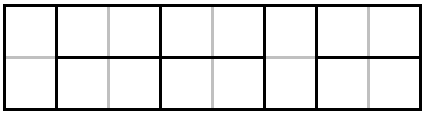
\includegraphics[width=2in]{quiz-09/domino-tiling.png}}
\caption{\label{fig:domino-tiling} Domino Tiling.}
\end{figure}


In your answer write the recurrent expression of {\tt a(n)} (express it through the previous members
of the sequence: {\tt a(n-1),...}).

{\em Note.} Assume that all the little
chocolate squares are distinguishable; the cuts that differ by 
some symmetry (rotation or flip of the chocolate bar) are considered to be different.


\vspace{10pt}
{\bf Question 2.}
Somebody wants to find out, in how many ways it is possible to pay \$15 in a vending machine, using 
\$1 coins, \$1 bills, \$2 bills and \$5 bills, where the order, how you insert them into the machine matters.

In your answer write an integer number.

{\em Note.} In order to solve this, you probably want to define a 
recurrent sequence for $b_n$ and 
find $b_{15}$. People sometimes use characteristic functions for such problems as well:
see \url{https://bit.ly/2Qu4Re4}. Then they can solve some variations of this
problem (what happens, if you have limited number of \$5 bills, etc.), but they need to use
infinite power series and other calculus techniques.

\vspace{10pt}
{\bf Question 3.}
Consider a recurrent sequence: 
$$\left\{ \begin{array}{l}
a_0 = 0,\\
a_1 = 1, \\
a_n = 2a_{n-1} + 2a_{n-2},\;n\geq 2.\\
\end{array} \right.$$
Find both roots of the characteristic equation $r_1,r_2$. 

In you answer write two real numbers, round them to the nearest thousandth.


\vspace{10pt}
{\bf Question 4}
There is a sequence $a(n)$ such that $a(0) = 0$, $a(1) = 0$, $a(2)=1$, but its
characteristic equation is $(r-1)^2(r-2) = 0$. (See \url{https://bit.ly/3a72Ps0} where
the characteristic equations with repeated roots are explained.)
Find the value $a(8)$.

In your answer write a number. 


\vspace{10pt}
{\bf Question 5} 
Write the following expression:\\
{\tt ((A / (B - (C + D))) * E) - (F + (G + H))}\\
in prefix (Polish) notation and also in the postfix (reverse-Polish) notation. 

In your answer separate both expressions with a comma.



\vspace{10pt}
{\bf Question 6} 
Find the number of ways to parenthesize the following expression:\\
{\tt A / B - C + D * E - F + G + H}\\
You should not assume any associativity for the operations.
For example {\tt (F + G) + H} and {\tt F + (G + H)} are two 
different ways to insert parentheses. On the other hand
{\tt (F + G) + H} and {\tt ((F + (G)) + H)} is the same way, since 
the order of execution in both is the same.

In your answer write an integer number.


\vspace{10pt}
{\bf Question 7.} 
Suppose $f(n) = 3f(n/3) + 2n$, $f(1) = 1$. Find $f(3^8)$.

In your answer write an integer number.





\newpage

\subsection{Answers}

\vspace{4pt}
{\bf Question 1.} Answer: {\tt a(n)=a(n-1)+a(n-2)}\\
Notice that the leftmost two squares in the $2 \times n$ 
rectangle can be filled in two different ways:\\
{\bf Alternative 1:} They can be filled by a single vertical domino. 
In this case the remaining rectangle $2 \times (n-1)$ can be 
filled in $a(n-1)$ ways.\\
{\bf Alternative 2:} They can be filled by two horizontal dominoes.
In this case the remaining rectangle $2 \times (n-2)$ can be filled
in $a(n-2)$ ways.\\
The total number of ways is obtained by adding $a(n-1)$ and $a(n-2)$.

{\em Note.} The sequence $a(n)$ is a shifted Fibonacci sequence. 
We can easily verify that $a(n) = F_{n+1}$ for $n \geq 0$.
(We define $F_0 = 0$, $F_1 = 1$ and $F_{n} = F_{n-1} + F_{n-2}$ 
is the regular Fibonacci sequence.)

\vspace{6pt}
{\bf Question 2.} Answer: {\tt 527383}\\
Let us define the sequence $b_n$ (in how many ways you can 
insert \$1 coins, \$1 bills, \$2 bills and \$5 bills into a vending 
machine so that it adds up to $n$ dollars).\\
But before that we consider a simpler sequence $a_n$ (in how many ways you can 
insert \$1 coins, \$1 bills, \$2 bills into a vending machine to pay $n$ dollars \textendash{}
i.e.\ you do not use \$5 bills at all). 

Sequence $a_n$ was already discussed in the {\em Sample Quiz 9}, Problem 2. 
It is defined as a recurrent sequence:
$$\left\{ \begin{array}{l}
a_1 = 2, \\
a_2 = 5, \\
a_{n} = 2a_{n-1} + a_{n-2},\;n \geq 3.\\
\end{array} \right.$$

If you wish, you can also define $a_0 = 1$ (there is exactly one way how to pay \$0 \textendash{}
use zero instances of every coin and bill). Compute the initial members of this sequence:
$$(a_1,a_2,a_3,a_4) = (2,5,12,29).$$

Notice that the sequence $b_n$ (where we also allow \$5 bills) would have exactly same 
members up to $b_4$ (because sums up to $4$ dollars cannot use any \$5 bills anyway).
Further members of $b_n$ can be defined recursively:
$$\left\{ \begin{array}{l}
b_0 = 1,\\
b_1 = 2,\\
b_2 = 5,\\
b_3 = 12,\\
b_4 = 29,\\
b_n = 2b_{n-1} + b_{n-2} + b_{n-5},\;n \geq 5.\\
\end{array} \right.$$

The last (recurrent) line means that $b_n$ ($n \geq 5$) is a total of four different kinds of sequences:
\begin{itemize}
\item Some sequences start from a \$1 coin; the rest is paid in $b_{n-1}$ different ways.
\item Some sequences start from a \$1 bill; the rest is paid in $b_{n-1}$ different ways.
\item Some sequences start from a \$2 bill; the rest is paid in $b_{n-2}$ different ways.
\item Some sequences start from a \$5 bill; the rest is paid in $b_{n-5}$ different ways.
\end{itemize}

Here are the first members $b_0,\ldots,b_{15}$ of this sequence:

$1,\; 2,\; 5,\; 12,\; 29,\; 71,\; 173,\; 422,\; 1029,\; 2509,\; 6118,$
$14918,\; 36376,\; 88699,\; 216283,\; 527383$.




\vspace{6pt}
{\bf Question 3.} Answer:\\ {\tt 2.732,-0.732} or 
{\tt -0.732,2.732} \\
The characteristic equation is 
$$r^2 - 2r - 2 = 0.$$
And the roots of this square equation are 
$r_{1,2} = 1 \pm \sqrt{3}$.
By rounding them to the nearest thousandth, we get
the answer. 

{\em Note.} By the way, we can also 
find the formula for $a_n$. (See {\em Sample Quiz 9}, 
Problem 3, {\bf (B)}.)

\vspace{6pt}
{\bf Question 4} Answer: {\tt 247}\\
Rewrite the characteristic equation:
\begin{align}
(r-1)^2(r-2) & = (r^2 - 2r + 1)(r-2) = \nonumber \\
 & = r^3 - 2r^2 + r - 2r^2 + 4r - 2 = \nonumber \\
 & = r^3 - 4r^2 + 5r - 2 = 0. \nonumber
\end{align}
We can restore the recurrent relationship from here: 
$$a_{n} = 4a_{n-1} - 5a_{n-2} + 2a_{n-3}.$$

\begin{tabular}{|c|r|r|r|r|r|r|r|r|r|} \hline
$n$   & 0 & 1 & 2 & 3 & 4  & 5  & 6  & 7   & 8 \\ \hline
$a_n$ & 0 & 0 & 1 & 4 & 11 & 26 & 57 & 120 & 247 \\ \hline
\end{tabular}


\vspace{6pt}
{\bf Question 5} Answer:\\ 
{\tt -*/A-B+CDE+F+GH, ABCD+-/E*FGH++-}\\
In order to transform infix notation into postfix notation
we can do this step by step. We start with the last/outermost operation
(minus in our case). And leave both subexpressions in 
the infix form. Then we find the last/outermost operation 
the subexpressions and so on.

{\tt ((A/(B-(C+D)))*E) - (F+(G+H))}\\
{\tt \textcolor{red}{-} ((A/(B-(C+D)))*E) (F+(G+H))}\\
{\tt \textcolor{red}{- *} (A/(B-(C+D))) E (F+(G+H))}\\
{\tt \textcolor{red}{- * /} A (B-(C+D)) E (F+(G+H))}\\
{\tt \textcolor{red}{- * /} A \textcolor{red}{-} B (C+D) E (F+(G+H))}\\
{\tt \textcolor{red}{- * /} A \textcolor{red}{-} B \textcolor{red}{+} C D E (F+(G+H))}\\
{\tt \textcolor{red}{- * /} A \textcolor{red}{-} B \textcolor{red}{+} C D E \textcolor{red}{+} F (G+H)}\\
{\tt \textcolor{red}{- * /} A \textcolor{red}{-} B \textcolor{red}{+} C D E \textcolor{red}{+} F \textcolor{red}{+} G H}\\

In these expressions the regular (infix) arithmetic operations are shown in black, but 
prefix arithmetic operations are shown in red. Postfix transformation is very similar.



\vspace{6pt}
{\bf Question 6} Answer: {\tt 429}\\ 
The expression {\tt A/B-C+D*E-F+G+H} contains
$7$ operations and $8$ operands/letters. It can 
be parenthesized in $C_7 = 429$ ways, where
$C_n$ is the sequence of {\em Catalan numbers}
defined recursively: 
$$\left\{ \begin{array}{l}
C_0 = 1, \\
C_{n+1}=\sum\limits_{i=0}^{n} C_i \cdot C_{n-i} 
\end{array} \right.$$

Here are the first few members:\\
$C_0=1,\; C_1=1,\; C_2=2,\; C_3=5,\; C_4=14,\; C_5=42,$\\
$C_6=132,\; C_7=429,\; C_8=1430,\; C_9=4862,$\\
$C_{10}=16796.$


\vspace{6pt}
{\bf Question 7} Answer: {\tt 111537}\\
We can compute the subsequent values, using the recursive formula.

\begin{tabular}{|l|l|} \hline
$n$ & $f(n)$ \\ \hline
$3^0$ & $1$ \\ \hline
$3^1$ & $9 = 3 \cdot 3$ \\ \hline
$3^2$ & $45 = 5 \cdot 9$ \\ \hline
$3^3$ & $189 = 7 \cdot 27$ \\ \hline
$3^4$ & $729 = 9 \cdot 81$ \\ \hline
$3^5$ & $2673 = 11 \cdot 243$ \\ \hline
$3^6$ & $9477 = 13 \cdot 729$ \\ \hline
$3^7$ & $32805 = 15 \cdot 2187$ \\ \hline
$3^8$ & $111537 = 17 \cdot 6561$ \\ \hline
\end{tabular}

It is possible to prove by induction that\\ $f(n) = (2n+1) \cdot 3^n$.\\
We can also apply this theorem:

{\bf Master Theorem:} Let $f$ be an increasing function that 
satisfies the recurrence relation
$$f(n) = af(n/b) + cn^d$$
whenever $n = b^k$, where $k$ is a positive integer greater than 
$1$, and $c$  and $d$ are real numbers with $c$ positive 
and $d$ nonnegative. Then
$$f(n)\;\text{is}\;\left\{ \begin{array}{ll}
O\left(n^d\right) & \text{if}\;a<b^d \\
O\left(n^d \log n \right) & \text{if}\;a=b^d \\
O\left(n^{\log_b a}\right) & \text{if}\;a>b^d \\
\end{array} \right.$$

In our case $a = 3$, $b = 3$, $c=2$ and $d = 1$. 
Observe that $a = b^d$, therefore we get that $f(n)$ is in 
$O(n \log n)$.\\

For example, if $n = 3^8 = 6561$, then $f(n) = 6561 \cdot 17$. 
We clearly see both factors: $6561$ grows as $O(n)$, but
$17 = 2 \cdot \left( \log_3 6561 \right) +1$ grows as $O(\log n)$ (we do not care about the
base of a logarithm in the Big-O notation). So their product 
$f(n)$ grows as $O(n \log n)$.




\end{document}





\newpage
\documentclass[jou]{apa6}

\usepackage[american]{babel}

\usepackage{csquotes}
\usepackage[style=apa,sortcites=true,sorting=nyt,backend=biber]{biblatex}
\DeclareLanguageMapping{american}{american-apa}
\addbibresource{bibliography.bib}


%%%%%%%%%%%%%%%%%%%%%%%%%%%%%%%%%%%%%%%%
%% Discrete Structures
%% The start of RBS stuff
%%%%%%%%%%%%%%%%%%%%%%%%%%%%%%%%%%%%%%%%

% Working internal and external links in PDF
\usepackage{hyperref}
% Extra math symbols in LaTeX
\usepackage{amsmath}
\usepackage{gensymb}
\usepackage{amssymb}
% Enumerations with (a), (b), etc.
\usepackage{enumerate}

\let\OLDitemize\itemize
\renewcommand\itemize{\OLDitemize\addtolength{\itemsep}{-6pt}}

\usepackage{etoolbox}
\makeatletter
\preto{\@verbatim}{\topsep=3pt \partopsep=3pt }
\makeatother

% These sizes redefine APA for A4 paper size
\oddsidemargin 0.0in
\evensidemargin 0.0in
\textwidth 6.27in
\headheight 1.0in
\topmargin -24pt
\headheight 12pt
\headsep 12pt
\textheight 9.19in



\title{Sample Quiz 8}
\author{Discrete Structures, Spring 2020}
\affiliation{RBS}

\leftheader{Discrete Sample Quiz 8}

\abstract{%
}

%\keywords{}

\setlength\parindent{0pt}

\begin{document}

%\thispagestyle{empty}

\twocolumn
\section{Worksheet 10: Binary Relations}

\vspace{6pt}
{\bf Question 1 (A reminiscence about variance)}\\
Assume that you want to encode six-letter alphabet 
$\mathcal{A} = \{ \mathtt{a}, \mathtt{b}, \mathtt{c}, \mathtt{d}, \mathtt{e}, \mathtt{f} \}$
and transmit it over a computer network.
You assign $2$ or $3$ bit codes to these letters: 

\begin{tabular}{|l|l|} \hline
{\tt a} & {\tt 00} \\ \hline
{\tt b} & {\tt 01} \\ \hline
{\tt c} & {\tt 100} \\ \hline
{\tt d} & {\tt 101} \\ \hline
{\tt e} & {\tt 110} \\ \hline
{\tt f} & {\tt 111} \\ \hline
\end{tabular}

For example, the 11-bit sequence {\tt "10100100110"} means {\tt "dace"}.
Denote by $X$ the random variable \textendash{} the number of 
bits used to encode a single letter. (All $6$ letters have 
equal probabilities.)

Find $E(X)$ and $V(X)$.\\
Write them as two fractions: {\tt P1/Q1,P2/Q2}\\
(Separate the fractions by comma, 
do not leave any spaces.)


\vspace{6pt}
{\bf Question 2 (Rosen7e, Ch.9, Q10-Q23).}\\
Determine whether the binary relation is: (1) reflexive, (2) symmetric, (3) antisymmetric, (4) transitive.
Express your answer as as a 4-letter string of T/F (true/false values that are 
answer to these $4$ questions). For example, {\tt TFTT} etc.
%For example, the relationship $a \leq b$ on $\mathbb{Z}$ has these answers: {\tt TFTT}. It is reflexive, antisymmetric
%and transitive. But $\leq$ is not symmetric ($a \leq b$ does not imply that $b \leq a$).
\begin{enumerate}[(A)]
\item The relation $R$ on $\{1, 2, 3,\ldots\}$ where $aRb$ means $a\,\mid\,b$.
\item The relation $R$ on $\{w, x, y, z\}$ where $R = \{(w, w), (w, x), (x, w), (x, x), (x, z), (y, y), (z, y), (z, z)\}$.
\item The relation $R$ on $\mathbb{Z}$ where $aRb$ means $|a - b| \leq 1$.
\item The relation $R$ on $\mathbb{Z}$ where $aRb$ means $a \neq b$.
\item The relation $R$ on $\mathbb{Z}$ where $aRb$ means that the units digit of $a$ is equal to the units digit of $b$.
\item The relation $R$ on the set of all subsets of $\{1, 2, 3, 4\}$ where $SRT$ means $S \subseteq T$.
\item The relation $R$ on the set of all people where $aRb$ means that a is younger than $b$.
\item The relation $R$ on the set $\{(a, b) \,\mid\, a, b \in \mathbb{Z}\}$ where $(a, b)R (c, d)$ means $a = c$ or $b = d$.
\end{enumerate}

\vspace{6pt}
{\bf Question 3 (Rosen7e, Ch.9, Q35-Q38).}\\
Construct a matrix of the relations defined below. Output the matrix as a list of lists:\\
{\tt [[a11,a12,...],[a21,a22,...],...]}
\begin{enumerate}[(A)]
\item $R$ on $\{1, 2, 3, 4, 6, 12\}$ where $aRb$ means $a\,\mid\,b$.
\item $R$ on $\{1, 2, 3, 4, 6, 12\}$ where $aRb$ means $a \leq b$.
\item $R^2$, where $R$ is the relation on $\{1, 2, 3, 4\}$ such that $aRb$ 
means $|a - b| \leq 1$.
\end{enumerate}

\vspace{6pt}
{\bf Question 4 (Rosen7e, Ch.9, Q42).}\\
Define
$$M_R = \left( \begin{array}{cccc}
1 & 0 & 1 & 0 \\
1 & 0 & 0 & 1 \\
1 & 1 & 1 & 0 \\
1 & 1 & 0 & 1 \\
\end{array} \right)$$
determine if $R$ is: (1) reflexive (2) symmetric (3) antisymmetric (4) transitive.
Express your answer as as a 4-letter string of T/F (true/false values that are 
answer to these $4$ questions). For example, 
{\tt TFTT} etc.


\vspace{6pt}
{\bf Question 5 (Rosen7e, Ch.9, Q47).}\\
Let $A$ be the set of all positive divisors of $60$ (including $1$ and $60$ itself). 
Draw the Hasse diagram for the relation $R$ on $A$ where $aRb$ means $a\,\mid\,b$.

\vspace{6pt}
{\bf Question 6 (Rosen7e, Ch.9, Q51).}\\
Find the transitive closure of $R$ if 
$$M_R  = \left( \begin{array}{cccc}
1 & 0 & 1 & 0 \\
1 & 0 & 0 & 1 \\
0 & 1 & 1 & 0 \\
0 & 1 & 0 & 0 \\
\end{array} \right).$$

\vspace{6pt}
{\bf Question 7 (Rosen7e, Ch.9, Q59).}\\
Find the join of the 3-ary relation:
\begin{verbatim}
{ (Wages,MS410,N507),
  (Rosen,CS540,N525),
  (Michaels,CS518,N504),
  (Michaels,MS410,N510) }
\end{verbatim}
and the 4-ary relation:
\begin{verbatim}
{ (MS410,N507,Monday,6:00), 
  (MS410,N507,Wednesday,6:00), 
  (CS540,N525,Monday,7:30),
  (CS518,N504,Tuesday,6:00), 
  (CS518,N504,Thursday,6:00) }
\end{verbatim}
with respect to the last two fields of the first relation and 
the first two fields of the second relation. 

\vspace{6pt}
{\bf Question 8 (Rosen7e, Ch.9, Q69-Q71).}
Give an example of a relation or state that there are none.\\
{\bf (A)} A relation on $\{a, b, c\}$ that is reflexive and transitive, but not antisymmetric.\\
{\bf (B)} A relation on $\{1, 2\}$ that is symmetric and transitive, but not reflexive.\\
{\bf (C)} A relation on $\{1, 2, 3\}$ that is reflexive and transitive, but not symmetric.

\vspace{6pt}
{\bf Question 9 (Rosen7e, Ch.9, Q73).}\\
Suppose $|A| = 7$. Find the number of reflexive, symmetric binary relations on $A$.





\newpage

\subsection{Answers}


\vspace{6pt}
{\bf Question 1.} 
The random variable $X$ takes value $x_1 = 2$ (with probability $p_1 = \frac{1}{3}$)
and value $x_2 = 3$ (with probability $p_2 = \frac{2}{3}$). 
We can compute: 
$$E(X) = x_1p_1 + x_2p_2 = \frac{8}{3}.$$
$$V(X) = (x_1 - E(X))^2p_1 + (x_2 - E(X))^2p_2 = \frac{2}{9}.$$

\vspace{6pt}
{\bf Question 2.} 
\begin{enumerate}[(A)]
\item {\tt TFTT}
\item {\tt TFFF}
\item {\tt TTFF}
\item {\tt FTFF}
\item {\tt TTFT}
\item {\tt TFTT}
\item {\tt FFTT}
\item {\tt TTFF}
\end{enumerate}

\vspace{6pt}
{\bf Question 3.}\\
{\bf (A)} Divisibility on the set $\{1, 2, 3, 4, 6, 12\}$
$$M_R  = \left( \begin{array}{cccccc}
1 & 1 & 1 & 1 & 1 & 1 \\
0 & 1 & 0 & 1 & 1 & 1 \\
0 & 0 & 1 & 0 & 1 & 1 \\
0 & 0 & 0 & 1 & 0 & 1 \\
0 & 0 & 0 & 0 & 1 & 1 \\
0 & 0 & 0 & 0 & 0 & 1 \\
\end{array} \right).$$
{\bf (B)} Relation $\leq$ on the set $\{1, 2, 3, 4, 6, 12\}$
$$M_R  = \left( \begin{array}{cccccc}
1 & 1 & 1 & 1 & 1 & 1 \\
0 & 1 & 1 & 1 & 1 & 1 \\
0 & 0 & 1 & 1 & 1 & 1 \\
0 & 0 & 0 & 1 & 1 & 1 \\
0 & 0 & 0 & 0 & 1 & 1 \\
0 & 0 & 0 & 0 & 0 & 1 \\
\end{array} \right).$$
{\bf (C)} Relation $R^2$, where $aRb$ iff $|a-b| \leq 1$.
$$M_R  = \left( \begin{array}{cccc}
1 & 1 & 1 & 0 \\
1 & 1 & 1 & 1 \\
1 & 1 & 1 & 1 \\
0 & 1 & 1 & 1 \\
\end{array} \right).$$
The only pairs that do not belong to $R^2$ are 
$(1;4)$ and $(4;1)$. 




\vspace{6pt}
{\bf Question 4.} Answer: {\tt FFFF}\\
Imagine that the relation $R$ is defined on a set of these 4 elements:
$a,b,c,d$. 
\begin{itemize}
\item $R$ is not reflexive, since $bRb$ is false (the matrix has $m_{22}=0$).
\item $R$ is not symmetric, since $bRa$ does not imply $aRb$
(the matrix has $m_{12}=0$, but $m_{21}=1$).
\item $R$ is not antisymmetric, since $aRc$ and $cRa$ both hold, but 
$a \neq c$.
\item $R$ is not transitive, since $aRc$ and $cRb$, but $aRb$ is not true.
\end{itemize}

\vspace{6pt}
{\bf Question 5}:\\
Hasse diagram connects only those numbers $a,b$ where $a$ divides $b$, and
there is no third  number in-between (such that $a\,\mid\,c$ and $c\,\mid\,b$). 
For example, $1$ and $2$ are connected, but $1$ and $4$ are not 
(because the relation $1\,\mid\,4$ can be inferred from 
$1\,\mid\,2$ and $2\,\mid\,4$).

\begin{figure}[!htb]
\center{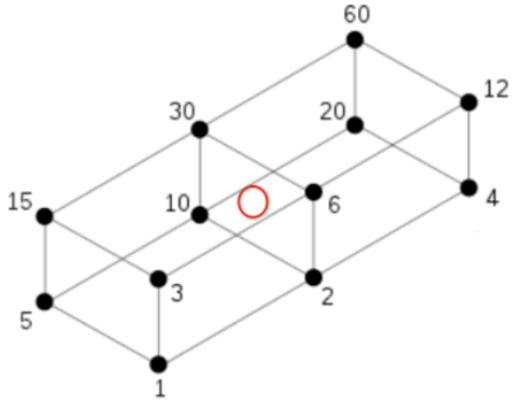
\includegraphics[width=2.5in]{quiz-sample-10/hasse-diagram-60.png}}
\caption{\label{fig:hasse-diagram-60} Hasse diagram: Divisors of 60.}
\end{figure}

Note that the Hasse diagram for divisibility is centrally symmetric. 
(This is true for any set of divisors for some number.)


\vspace{6pt}
{\bf Question 6}:\\
$$M_R  = \left( \begin{array}{cccc}
1 & 0 & 1 & 0 \\
1 & 0 & 0 & 1 \\
0 & 1 & 1 & 0 \\
0 & 1 & 0 & 0 \\
\end{array} \right).$$

Denote the elements of the set by $a,b,c,d$. We want to find, 
what are the ``relational paths'' between them:
\begin{itemize}
\item Path $aRc$, $cRb$, $bRd$ adds $(a,b)$, $(a,d)$ to the transitive closure.
\item Path $bRa$, $aRc$, $cRb$ adds $(b,c)$, $(b,b)$ to the transitive closure.
\item Path $cRb$, $bRd$ adds $(c,d)$ to the transitive closure.
\item Path $cRb$, $bRa$ adds $(c,a)$ to the transitive closure.
\item Path $dRb$, $bRa$, $aRc$ adds $(d,a)$, $(d,c)$.
\item Path $dRb$, $bRd$ adds $(d,d)$.
\end{itemize}

Here is the matrix 
of the transitive closure after all the new pairs are added:

$$M_{R\ast}  = \left( \begin{array}{cccc}
1 & 1 & 1 & 1 \\
1 & 1 & 1 & 1 \\
1 & 1 & 1 & 1 \\
1 & 1 & 1 & 1 \\
\end{array} \right).$$



\vspace{6pt}
{\bf Question 7}\\
TBD (see Section 9.2.4 of the textbook (Definition 4, page 615)). This problem 
is based entirely on applying the definition.

\vspace{6pt}
{\bf Question 8}\\
{\bf (A)} TBD\\
{\bf (B)}. Yes. We can have a relation $R$ which is 
never satisfied. It is symmetric and also transitive
(since $xRy$ and $yRz$ can never happen, so we do not
need to care about $xRz$).\\
{\bf (C)}. TBD.


\vspace{6pt}
{\bf Question 9} Answer: {\tt 2097152}\\
The matrix $M$ of any relation $R$ on a set of $7$ elements has $49$ entries. 
The entries on the main diagonal ($m_{11},m_{22},\ldots,m_{77}$) 
should all equal $1$ ($R$ is reflexive). 
Also, any entry $m_{ij}$ above the main diagonal ($i<j$ - row number is
less than the column number) is symmetric to some entry below the diagonal
$m_{ji}$ (where $i>j$). 

Therefore we can freely choose only those $m_{ij}$ that are above the main 
diagonal; everything else is predetermined. There are $1+2+\ldots+6=21$ such 
elements in the matrix. The total number of ways to choose them is
$2^{21} = 2097152$.




\end{document}



\newpage
\documentclass[jou]{apa6}

\usepackage[american]{babel}

\usepackage{csquotes}
\usepackage[style=apa,sortcites=true,sorting=nyt,backend=biber]{biblatex}
\DeclareLanguageMapping{american}{american-apa}
\addbibresource{bibliography.bib}


%%%%%%%%%%%%%%%%%%%%%%%%%%%%%%%%%%%%%%%%
%% Discrete Structures
%% The start of RBS stuff
%%%%%%%%%%%%%%%%%%%%%%%%%%%%%%%%%%%%%%%%

% Working internal and external links in PDF
\usepackage{hyperref}
% Extra math symbols in LaTeX
\usepackage{amsmath}
\usepackage{gensymb}
\usepackage{amssymb}
% Enumerations with (a), (b), etc.
\usepackage{enumerate}

\let\OLDitemize\itemize
\renewcommand\itemize{\OLDitemize\addtolength{\itemsep}{-6pt}}

\usepackage{etoolbox}
\makeatletter
\preto{\@verbatim}{\topsep=3pt \partopsep=3pt }
\makeatother

% These sizes redefine APA for A4 paper size
\oddsidemargin 0.0in
\evensidemargin 0.0in
\textwidth 6.27in
\headheight 1.0in
\topmargin -24pt
\headheight 12pt
\headsep 12pt
\textheight 9.19in



\title{Sample Quiz 8}
\author{Discrete Structures, Spring 2020}
\affiliation{RBS}

\leftheader{Discrete Quiz 10}

\abstract{%
}

%\keywords{}

\setlength\parindent{0pt}

\begin{document}

%\thispagestyle{empty}

\twocolumn
\section{Quiz 10: Binary Relations}

\vspace{6pt}
{\bf Question 1}\\
Some people participate in an Einkaufshelden program \textendash{} they 
go to one of the shops $A$, $B$ or $C$ and deliver the products to the endpoints
$X$, $Y$ or $Z$. Each of the $9$ edges is selected by the same probability 
(Figure~\ref{fig:k33-weights})

\begin{figure}[!htb]
\center{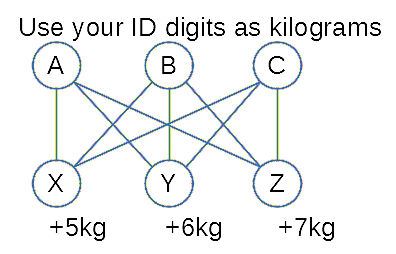
\includegraphics[width=2in]{quiz10/k33-weights.png}}
\caption{\label{fig:k33-weights} The Paths of a Delivery Service.}
\end{figure}


The sum of the numbers on both ends of an edge shows 
how many kilograms of stuff were delivered. (For example, if your Student ID has 
$A=0$, then on $AZ$ there are $0+7 = 7$ kilograms.
Let $X$ denote the random variable: the kilograms of stuff delivered
on a single edge.

Write the variance $V(X)$ as an irreducible fraction {\tt P/Q}. 


\vspace{6pt}
{\bf Question 2.}\\
Given a set of the first positive integers $S = \{ 1,2,\ldots,A+B+(10-C) \}$
(where {\tt A,B,C} are the digits from your student ID). 
We define a relation on $S$: $aRb$ is true iff $|a - b| \leq 2$.

Let $R^2$ be the second power of that relation $R$ and let $M_{R^2}$
be its matrix. Find the number of 1s in this matrix (In other words: 
how many pairs belong to this relation?)


\vspace{6pt}
{\bf Question 3.}\\
Define a set $S$ of these six positive integers: 
\begin{align}
S = \{ & 1+\mathtt{A},\; 2+\mathtt{A}+\mathtt{B},\; 3+\mathtt{A}+\mathtt{B}+\mathtt{C},\;
4 + 2\mathtt{A}+\mathtt{B}+\mathtt{C},\; \nonumber \\
 & 5 + 2\mathtt{A}+2\mathtt{B}+\mathtt{C},\;
6 + 2\mathtt{A}+2\mathtt{B}+2\mathtt{C}\}. \nonumber
\end{align}

Now compute the remainders of the elements of $S$ when divided by $16$. 
You should get another set $S'$ where each element is between $0$ and $15$. 
($S'$ may contain fewer elements than $S$, if some remainders are identical.)
Let $b_i$ be a sequence of bits ($i = 0,\ldots,15$):
$$b_i = 1\;\text{iff}\;i \in S'.$$

We define a matrix for relation $R$ as follows:
$$M_R = \left( \begin{array}{cccc}
b_{0} & b_1 & b_2 & b_3 \\
b_{4} & b_5 & b_6 & b_7 \\
b_{8} & b_9 & b_{10} & b_{11} \\
b_{12} & b_{13} & b_{14} & b_{15} \\
\end{array} \right)$$
Let $M^{\ast}$ be the matrix of the transitive closure of $R$. 
Find the number of 1s in the matrix $M^{\ast}$.


\vspace{6pt}
{\bf Question 4.}\\
Let $S$ be a set and its size is computed from the digits in your ID:
$$|S| = \mathtt{A}+\mathtt{B}+(10 - \mathtt{C}).$$ 
Let $N$ be the number of binary relations on $S$ that are  
reflexive and symmetric at the same time.
Write the last $3$ digits of $N$ in your answer.

{\em Hint} If you need to find the last $3$ digits of some large number, you 
can use periodicity (similar to this: \url{https://bit.ly/33NrJKI}). Euler's theorem 
about the period of remainders modulo $1000$ being periodic with period $\varphi(1000)$ 
(see \url{https://bit.ly/33PyI5Q}) is not directly applicable in this situation,
since your exponent $a$ is not mutually prime with $1000$.
But with some additional reasoning you 
can use Euler's theorem as well.


\vspace{6pt}
{\bf Question 5.}\\
Find the join of the 3-ary relation:
\begin{verbatim}
{ (Wages,MS410,N507),
  (Rosen,CS540,N525),
  (Michaels,CS518,N504),
  (Michaels,MS410,N510) }
\end{verbatim}
and the 4-ary relation:
\begin{verbatim}
{ (MS410,N507,Monday,6:00), 
  (MS410,N507,Wednesday,6:00), 
  (CS540,N525,Monday,7:30),
  (CS518,N504,Tuesday,6:00), 
  (CS518,N504,Thursday,6:00) }
\end{verbatim}
with respect to the last two fields of the first relation and 
the first two fields of the second relation. 

Write the number records in the join.

\vspace{6pt}
{\bf Question 6.}\\
Let $R$ be a relation on the set $\{x_1,x_2,x_3\}$ that is reflexive and transitive, but not antisymmetric.
Denote its matrix by
$$M_R =  \left( \begin{array}{ccc}
b_{11} & b_{12} & b_{13} \\
b_{21} & b_{22} & b_{23} \\
b_{31} & b_{32} & b_{33} \\
\end{array} \right)$$

Write all the 9 bits (as a sequence of 0s and 1s) in your answer: $b_{11}b_{12}b_{13}b_{21}b_{22}b_{23}b_{31}b_{32}b_{33}$.
If there are multiple answers, write the lexicographically first one. 



\vspace{6pt}
{\bf Question 7.}\\
Let $R$ be a relation on $\{a, b, c\}$ that is reflexive and transitive, but not symmetric.
Denote its matrix by
$$M_R =  \left( \begin{array}{ccc}
b_{11} & b_{12} & b_{13} \\
b_{21} & b_{22} & b_{23} \\
b_{31} & b_{32} & b_{33} \\
\end{array} \right)$$

Write all the 9 bits (as a sequence of 0s and 1s) in your answer: $b_{11}b_{12}b_{13}b_{21}b_{22}b_{23}b_{31}b_{32}b_{33}$.
If there are multiple answers, write the lexicographically first one. 




\newpage

\subsection{Answers}

In solutions we assume that $A = 4$, $B = 5$, $C = 6$. 

\vspace{6pt}
{\bf Question 1.} Answer: {\tt 7} (if $A = 4$, $B = 5$, $C = 6$)\\ 

Figure~\ref{fig:k33-weights-456} shows all the weight combinations in this case. 
The list of total weights on all $9$ edges is the following: 
$$x_1 = 9,\;10,\;11,\;10,\;11,\;12,\;11,\;12,\;x_9 = 13.$$
The mean value is $11$. Variance $V(X)$ is the arithmetic mean of all squared deviations from that mean:
$$V(X) = \frac{\sum_{i=1}^9 (x_i - 11)^2}{9} = \frac{12}{9} = \frac{4}{3}.$$

Therefore $m+n = 4+3 = 7$.

\begin{figure}[!htb]
\center{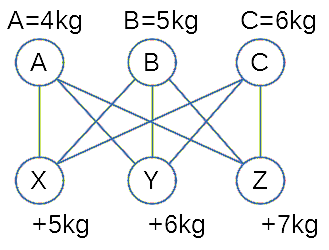
\includegraphics[width=1.6in]{quiz10/k33-weights-456.png}}
\caption{\label{fig:k33-weights-456} Delivery Service (specific values).}
\end{figure}


\vspace{6pt}
{\bf Question 2.} Answer: {\tt 97} (if $A = 4$, $B = 5$, $C = 6$)\\ 
$S = \{ 1,2,\ldots,A + B + (10-C) \} = \{ 1,2,\ldots,13 \}$,\\
The relation $R^2$ on any two $a,b \in S$ holds, iff 
the distance between $a,b$ is no more than $4$.
This follows from the ``triangle inequality''. 

Namely, $a(R^2)b$ holds, if there exists $c$ that $aRc$ and $cRb$. 
Therefore $|a-c| \leq 2$ and $|c-b| \leq 2$ and we should have 
$|a - b| \leq 4$. The matrix of $R^2$ has $13 \times 13$ entries. 
Out of these entries the main diagonal (where $a=b$) and also 
other diagonal lines that run parallel to that contain $1$s.
The total number of $1$'s is 
$$9 + 10 + 11 + 12 + 13 + 12 + 11 + 10 + 9 = 97.$$







\vspace{6pt}
{\bf Question 3.} Answer: {\tt 16} (if $A = 4$, $B = 5$, $C = 6$)\\ 
Plug in the numbers $A,B,C$: 
$$S = \{ 5, 11, 18, 23, 29, 36 \},$$
$$S' = \{ 5, 11, 2, 7, 13, 4 \},$$
$$M_R = \left( \begin{array}{cccc}
0 & 0 & 1 & 0 \\
1 & 1 & 0 & 1 \\
0 & 0 & 0 & 1 \\
0 & 1 & 0 & 0 \\
\end{array} \right).$$

This matrix only contains $6$ elements equal to $1$, but its transitive
closure is all $16$ elements equal to $1$. Indeed, if we consider the relation $R$ 
on a set of four elements: $A = \{ a_1, a_2, a_3, a_4 \}$, then there is a cyclical path: 
$$a_1Ra_3,\;a_3Ra_4,\;a_4Ra_2,\;a_2Ra_1.$$
Therefore the transitive closure is a relation consisting of all pairs of elements $A \times A$. 



\vspace{6pt}
{\bf Question 4.} Answer: {\tt 544} (if $A = 4$, $B = 5$, $C = 6$)\\ 
We get $|S| =  A + B + (10 - C) = 13$. 
The matrix of any binary relation $R$ defined on $S$ has $13 \times 13 = 169$ elements. 
Since $R$ is reflexive, all the elements on the main diagonal of that matrix are equal to $1$. 
Moreover, any elements above the diagonal are symmetric to some element below the main diagonal. 
Ultimately, we can only choose $(169 - 13)/2 = 78$ elements in the matrix. 
Each element can have two values, therefore $N = 2^{78}$. 

The last three digits in that number are $544$. 
Indeed,
$$\left\{ \begin{array}{l}
2^{78} \equiv 0\; (\text{mod}\; 8), \\
2^{78} \equiv 44\;(\text{mod}\; 125). \\
\end{array} \right.$$

The first congruence is obvious (any large power of $2$ is divisible by $8$). 
The second one follows from 
\begin{align}
2^{78} & = 2^{64} \cdot 2^{8} \cdot 2^{4} \cdot 2^{2} \equiv  \nonumber \\
  & \equiv 116 \cdot 6 \cdot 16 \cdot 4 = \nonumber \\
  & = 44544 \equiv 44 \;(\text{mod}\; 125) \nonumber
\end{align}

\vspace{6pt}
{\bf Question 5.} Answer: {\tt 5}\\ 

{\footnotesize
\begin{tabular}{|l||ll||ll|} \hline
{\bf Table1} & {\bf Joined} &  & {\bf Table2} & \\ \hline
(T1.L1) Wages & MS410 & N507 & (T2.L1) Mon & 6:00 \\ \hline
(T1.L1) Wages & MS410 & N507 & (T2.L2) Wed & 6:00 \\ \hline
(T1.L2) Rosen & CS540 & N525 & (T2.L3) Mon & 7:30 \\ \hline
(T1.L3) Michaels & CS518 & N504 & (T2.L4) Tue & 6:00 \\ \hline
(T1.L3) Michaels & CS518 & N504 & (T2.L5) Thu & 6:00 \\ \hline
\end{tabular}
}

In this table the middle section shows the two joined columns. 
The left section shows the lines from Table 1 (with respective line numbers
in that table). The right section shows the lines from Table 2 (also with line numbers). 


\vspace{6pt}
{\bf Question 6.} Answer: {\tt 100011011}\\ 
We know that the relation is reflexive, so all the elements on its diagonal are $1$
($b_{11} = b_{22} = b_{33} = 1$). 
It must not be antisymmetric, so there must be $x \neq y$ such that $xRy$ and $yRx$. 
Since we want to have the lexicographically first matrix, we set the entries $b_{23}$ and
$b_{32} = 1$. The matrix is now as follows: 

$$M_R =  \left( \begin{array}{ccc}
1 & 0 & 0 \\
0 & 1 & 1 \\
0 & 1 & 1 \\
\end{array} \right)$$

We can easily verify that the relationship $R$ is also transitive (in fact, it is an 
equivalence relationship with two equivalence classes $\{x_1\}$ and
$\{x_2,x_3\}$). 



\vspace{6pt}
{\bf Question 7.} Answer: {\tt 100010011}\\
We know that the relation is reflexive, so all the elements on its diagonal are $1$
($b_{11} = b_{22} = b_{33} = 1$). 
It must not be symmetric, so we can set $b_{23} \neq b_{32}$. (In order to be 
the lexicographically first, we do not want to touch earlier entries in that matrix.)

$$M_R =  \left( \begin{array}{ccc}
1 & 0 & 0 \\
0 & 1 & 0 \\
0 & 1 & 1 \\
\end{array} \right)$$


\end{document}






\newpage
\documentclass[jou]{apa6}

\usepackage[american]{babel}

\usepackage{csquotes}
\usepackage[style=apa,sortcites=true,sorting=nyt,backend=biber]{biblatex}
\DeclareLanguageMapping{american}{american-apa}
\addbibresource{bibliography.bib}


%%%%%%%%%%%%%%%%%%%%%%%%%%%%%%%%%%%%%%%%
%% Discrete Structures
%% The start of RBS stuff
%%%%%%%%%%%%%%%%%%%%%%%%%%%%%%%%%%%%%%%%

% Working internal and external links in PDF
\usepackage{hyperref}
% Extra math symbols in LaTeX
\usepackage{amsmath}
\usepackage{gensymb}
\usepackage{amssymb}
% Enumerations with (a), (b), etc.
\usepackage{enumerate}

\let\OLDitemize\itemize
\renewcommand\itemize{\OLDitemize\addtolength{\itemsep}{-6pt}}

\usepackage{etoolbox}
\makeatletter
\preto{\@verbatim}{\topsep=3pt \partopsep=3pt }
\makeatother

% These sizes redefine APA for A4 paper size
\oddsidemargin 0.0in
\evensidemargin 0.0in
\textwidth 6.27in
\headheight 1.0in
\topmargin -24pt
\headheight 12pt
\headsep 12pt
\textheight 9.19in



\title{Sample Quiz 8}
\author{Discrete Structures, Spring 2020}
\affiliation{RBS}

\leftheader{Discrete Sample Quiz 8}

\abstract{%
}

%\keywords{}

\setlength\parindent{0pt}

\begin{document}

\thispagestyle{empty}

\twocolumn
{\Large Discrete Sample Quiz 11}

{\bf Question 1 (Rosen7e, Ch.10, Q11-Q14).}\\
{\bf (A)} $K_n$ (the complete graph on $n$ vertices) has $\ldots\ldots$ edges and $\ldots\ldots$ vertices.\\
{\bf (B)} $K_{m,n}$ (the complete bipartite graph on sets of sizes $m,n$) has $\ldots\ldots$ edges and $\ldots\ldots$ vertices.\\
{\bf (C)} $W_n$ (wheel graph on $n$ vertices \textendash{} $n$-gonal pyramid
viewed from above) has $\ldots\ldots$ edges and $\ldots\ldots$ vertices.\\
{\bf (D)} $Q_n$ ($n$-dimensional cube) has $\ldots\ldots$ edges and $\ldots\ldots$ vertices.

\vspace{10pt}
{\bf Question 2 (Rosen7e, Ch.10, Q15-Q17).}\\
{\bf (A)} The length of the longest simple circuit in $K_5$ is $\ldots\ldots$.\\
{\bf (B)} The length of the longest simple circuit in $W_{10}$ is $\ldots\ldots$.\\
{\bf (C)} The length of the longest simple circuit in $K_{4,10}$ is $\ldots\ldots$.

{\em Note.} A simple circuit in (Rosen2019) is defined as a circular
sequence of vertices $v_0,v_1,\ldots,v_n=v_0$, 
where each two vertices are connected by an edge
(and it does not contain any edge more than once).

\vspace{10pt}
{\bf Question 3 (Rosen7e, Ch.10, Q19-Q24).} In each example find 
the dimensions of a matrix; and number of 0s and 1s in it: Find $X,Y,Z,T$.\\
{\bf (A)} The adjacency matrix for $K_{m,n}$ has size (rows times columns)
$X \times Y$; it has $Z$ 0's and $T$ 1's.\\
{\bf (B)} The adjacency matrix for $K_n$  
has size $X \times Y$; it has $Z$ 0's and $T$ 1's.\\
{\bf (C)} The adjacency matrix for $C_n$  
has size $X \times Y$; it has $Z$ 0's and $T$ 1's.\\
{\bf (D)} The adjacency matrix for $Q_4$  
has size $X \times Y$; it has $Z$ 0's and $T$ 1's.\\
{\bf (E)} The incidence matrix for $W_n$ 
has size $X \times Y$; it has $Z$ 0's and $T$ 1's.\\
{\bf (F)} The incidence matrix for $Q_5$ 
has size $X \times Y$; it has $Z$ 0's and $T$ 1's.

{\em Note.} Adjacency matrix is a square matrix of size $|V| \times |V|$, 
but incidence matrix is a rectangular matrix of size $|V| \times |E|$.

\vspace{10pt}
{\bf Question 4 (Rosen7e, Ch.10, Q28-Q31).}\\
{\bf (A)} List all positive integers $n$ such that $K_n$ has an Euler circuit; 
what is its length in terms of $n$?\\
{\bf (B)} List all positive integers n such that Q n has an Euler circuit.



\vspace{10pt}
{\bf Question 5 (Rosen7e, Ch.10, Q43).}\\
If $G$ is a planar connected graph with $12$ regions and $20$ edges, then $G$ has $\ldots\ldots$ vertices.


\vspace{10pt}
{\bf Question 6 (Rosen7e, Ch.10, Q44).}\\
If $G$ is a planar connected graph with $20$ vertices, each of degree $3$, then $G$ has $\ldots\ldots$ regions.

\vspace{10pt}
{\bf Question 7 (Rosen7e, Ch.10, Q45).}\\
If a regular graph $G$ has $10$ vertices and $45$ edges, then each vertex of $G$ has degree $\ldots\ldots$.

{\em Note.} A {\em regular graph} is a graph where all vertices have the same degree.



\vspace{10pt}
{\bf Question 8 (Rosen7e, Ch.10, Q59-Q82).}\\
{\bf (A)} A simple graph with $6$ vertices, whose degrees are $2,2,2,3,4,4$.\\
{\bf (B)} A simple graph with $8$ vertices, whose degrees are $0,1,2,3,4,5,6,7$.\\
{\bf (C)} A simple graph with degrees $1,2,2,3$.\\
{\bf (D)} A simple graph with degrees $2,3,4,4,4$.\\
{\bf (E)} A simple graph with degrees $1,1,2,4$.\\
{\bf (F)} A simple digraph with indegrees $0,1,2$ and outdegrees $0,1,2$.\\
{\bf (G)} A simple digraph with indegrees $1,1,1$ and outdegrees $1,1,1$.\\
{\bf (H)} A simple digraph with indegrees $0,1,2,2$ and outdegrees $0,1,1,3$.\\
{\bf (I)} A simple digraph with indegrees $0,1,2,4,5$ and outdegrees $0,3,3,3,3$.\\
{\bf (J)} A simple digraph with indegrees $0,1,1,2$ and outdegrees $0,1,1,1$.\\
{\bf (K)} A simple digraph with indegrees: $0,1,2,2,3,4$ and outdegrees: $1,1,2,2,3,4$.\\
{\bf (L)} A simple graph with $6$ vertices and $16$ edges.\\
{\bf (M)} A connected simple planar graph with $5$ regions and $8$ vertices, each of degree $3$.\\
{\bf (N)} A graph with $4$ vertices that is not planar.\\
{\bf (O)} A planar graph with $10$ vertices.\\
{\bf (P)} A planar graph with $8$ vertices, $12$ edges, and $6$ regions.\\
{\bf (Q)} A planar graph with $7$ vertices, $9$ edges, and $5$ regions.



\vspace{10pt}
{\bf Question 9 (Rosen7e, Ch.10, Q108).}\\
Use Dijkstra’s Algorithm to find the shortest path length between 
the vertices a and z in these weighted graphs.

{\bf (A)}
\begin{center}
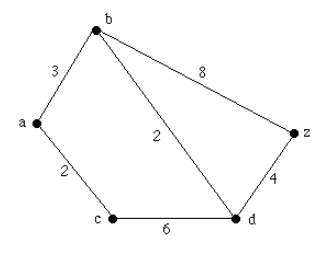
\includegraphics[width=2.8in]{dijkstra-graph1.png}
\end{center}

\newpage
{\bf (B)}
\begin{center}
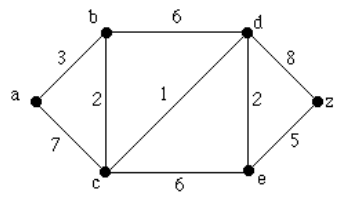
\includegraphics[width=2.8in]{dijkstra-graph2.png}
\end{center}



\vspace{10pt}
{\bf Question 10 (Rosen7e, Ch.10, Q113).}\\
The picture at the right shows the floor plan of
an office. Show that it is impossible to plan a walk that passes through
each doorway exactly once, starting and ending at $A$.
\begin{center}
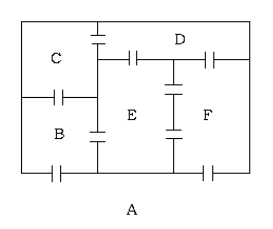
\includegraphics[width=2in]{floor-plan-graph.png}
\end{center}



\vspace{10pt}
{\bf Hall's Marriage Theorem (Rosen2019, p.772)}\\
The bipartite graph $G=(V,E)$ with partition 
of vertices into 2 disjoint sets $V = X \cup Y$ 
has a {\em maximum matching} that saturates $X$
iff for all $A \subseteq X$ we have
$|X| \leq |N(X)|$. 

{\em Note.} A {\em matching} in a graph is a set of of edges
such that no two edges share a common endpoint. 
A {\em maximum matching} is matching containing the greatest
number of edges. And a matching {\em saturates} a set $X$, 
if each vertex $v \in X$ belongs to some matching edge.

\vspace{10pt}
{\bf Question 11 (K\"{o}nig’s Marriage Theorem)}\\
Prove that if all the vertices of a bipartite graph
have the same degree, then it has a perfect matching.\\
(Quines2017, p.11); \url{https://cjquines.com/files/halls.pdf}

{\em Note.} A matching is {\em perfect}, if it saturates all vertices
(every vertex has a pair).

\vspace{10pt}
{\bf Question 12}\\
We have a regular deck of $52$ playing cards, with exactly $4$ cards of each of the
13 ranks. The cards have been randomly dealt into 13 piles, each with 4 cards in
it. Prove that there is a way to take a card from each pile so that after we take
a card from every pile, we have exactly a card of every rank.\\
(Quines2017, p.11).


\end{document}



\newpage
\documentclass[jou]{apa6}

\usepackage[american]{babel}

\usepackage{csquotes}
\usepackage[style=apa,sortcites=true,sorting=nyt,backend=biber]{biblatex}
\DeclareLanguageMapping{american}{american-apa}
\addbibresource{bibliography.bib}


%%%%%%%%%%%%%%%%%%%%%%%%%%%%%%%%%%%%%%%%
%% Discrete Structures
%% The start of RBS stuff
%%%%%%%%%%%%%%%%%%%%%%%%%%%%%%%%%%%%%%%%

% Working internal and external links in PDF
\usepackage{hyperref}
% Extra math symbols in LaTeX
\usepackage{amsmath}
\usepackage{gensymb}
\usepackage{amssymb}
% Enumerations with (a), (b), etc.
\usepackage{enumerate}
\usepackage{xcolor}

\let\OLDitemize\itemize
\renewcommand\itemize{\OLDitemize\addtolength{\itemsep}{-6pt}}

\usepackage{etoolbox}
\makeatletter
\preto{\@verbatim}{\topsep=3pt \partopsep=3pt }
\makeatother

% These sizes redefine APA for A4 paper size
\oddsidemargin 0.0in
\evensidemargin 0.0in
\textwidth 6.27in
\headheight 1.0in
\topmargin -24pt
\headheight 12pt
\headsep 12pt
\textheight 9.19in



\title{Sample Quiz 8}
\author{Discrete Structures, Spring 2020}
\affiliation{RBS}

\leftheader{Discrete Sample Quiz 8}

\abstract{%
}

%\keywords{}

\setlength\parindent{0pt}

\begin{document}

%\thispagestyle{empty}

\twocolumn
\section{Quiz 11: Graphs}

\vspace{4pt}
{\bf Question 1.}
Let $G = (V,E)$ be a graph, where $V$ is the set of all positive divisors of $144$ (including 
$1$ and $144$ itself). Two different vertices $d_1,d_2$ are connected by an edge iff one of the
numbers divides another ($d_1\,\mid\,d_2$ or $d_2\,\mid\,d_1$). 
Find the number of vertices $|V|$ and the number of edges $|E|$ in this graph.

Write two comma-separated integers.


\vspace{10pt}
{\bf Question 2.}
How long is the longest simple circuit in $W_{20}$? 
(A simple circuit is a circular path that may visit vertices multiple times, 
but does not contain any edge more than once.)

Write a positive integer. 




\vspace{10pt}
{\bf Question 3.}
Let $G$ be a planar connected graph with $60$ vertices, each vertex has degree $3$. 
How many regions are there in $G$?

Write a positive integer.



\vspace{10pt}
{\bf Question 4.} This is an adjacency matrix for some graph:
{\footnotesize
$$M_G = \left( 
\begin{array}{ccccccccc}
0 & 1 & 0 & 1 & 0 & 0 & 0 & 0 & 1 \\
1 & 0 & 1 & 1 & 1 & 0 & 0 & 0 & 0 \\
0 & 1 & 0 & 0 & 1 & 1 & 0 & 0 & 0 \\
1 & 1 & 0 & 0 & 1 & 0 & 1 & 0 & 0 \\
0 & 1 & 1 & 1 & 0 & 1 & 1 & 1 & 0 \\
0 & 0 & 1 & 0 & 1 & 0 & 0 & 1 & 1 \\
0 & 0 & 0 & 1 & 1 & 0 & 0 & 1 & 0 \\
0 & 0 & 0 & 0 & 1 & 1 & 1 & 0 & 1 \\
1 & 0 & 0 & 0 & 0 & 1 & 0 & 1 & 0 \\
\end{array} \right).$$
}

It is known that $G$ is a planar graph. Find the number of vertices $|V|$, 
number of edges $|E|$ and the number of regions $|R|$ for this graph. 

Write $3$ comma-separated integers.



\vspace{10pt}
{\bf Question 5 (Dudeney2016, Prob.434), ``536 Puzzles''.}

\begin{figure}[!htb]
\center{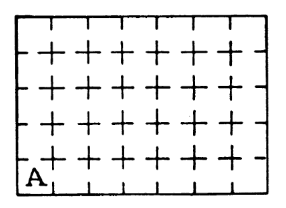
\includegraphics[width=1.5in]{quiz11/prison-cells.png}}
\caption{\label{fig:prison-cells} A weighted graph.}
\end{figure}

A prisoner currently is in the cell ``$A$'' (Figure~\ref{fig:prison-cells}). He has to visit each 
prison cell no more than once and return 
back to the cell ``$A$''. What is the largest number of prison cells that
can be visited in this way?\\
{\em (Visiting each cell once does not contradict with the requirement to return back 
to ``$A$'' \textendash{} the prisoner uses a circular path between the rooms: 
every room on the path, including ``$A$'', is entered once and left once. We want
to know the maximum length of this path.)}

Write a positive integer.

{\em Note.} You may also want to prove to yourself that the number is the largest possible.


\vspace{10pt}
{\bf Question 6}
There is a bipartite graph $G=(V,E)$ with exactly $|V| = 17$ vertices. (A graph is {\em bipartite}, if 
the set of vertices $V$ can be split into two parts $X$, $Y$ so that all edges are between a vertex in $X$ and a vertex in $Y$.)
Find the largest possible number of edges in such a graph. 

Write a positive integer.
 

\vspace{10pt}
{\bf Question 7} Verify, if these statements are true. 
A simple undirected graph is called a {\em cubic} graph, 
if every vertex has degree $3$.\\
{\bf (A)} There exists a cubic graph with $7$ vertices.\\
{\bf (B)} There exists a cubic graph with $6$ vertices that is not isomorphic to $K_{3,3}$.\\
{\bf (C)} There exists a cubic graph with $8$ edges.

Write a sequence of 3 comma-separated letters (e.g.\ {\tt T,T,T} or {\tt F,F,F}).




\vspace{10pt}
{\bf Question 8.} Verify, if these statements are true:\\
{\bf (A)} There exists a simple directed graph with indegrees $0,1,2,4,5$ and outdegrees $0,3,3,3,3$. (A graph is {\em simple}, if
it is not a {\em multigraph} \textendash{} there is no more than one edge $(u,v)$ for any vertices $u,v$.)\\
{\bf (B)} There exists a connected undirected simple planar graph with $5$ regions and $8$ vertices, each vertex has degree $3$.\\
{\bf (C)} There exists a connected undirected simple planar graph with $8$ regions and $6$ vertices, each region is surrounded 
with $3$ edges.

Write a sequence of 3 comma-separated letters (e.g.\ {\tt T,T,T} or {\tt F,F,F}).



\vspace{10pt}
{\bf Question 9.}
Use Dijkstra’s Algorithm to find the shortest paths from the source vertex $s$ 
to all other vertices $t,x,y,z$ (Figure~\ref{fig:dijkstra}). The length of a path is obtained by adding the 
weights of the directed edges.

\begin{figure}[!htb]
\center{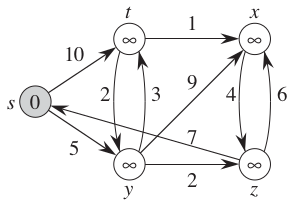
\includegraphics[width=1.8in]{quiz11/dijkstra.png}}
\caption{\label{fig:dijkstra} A weighted graph.}
\end{figure}


Write $4$ comma-separated numbers \textendash{} the shortest paths 
to the vertices $t,x,y,z$ respectively.

{\em Note.} Dijkstra's algorithm (Rosen2019, p.747) initializes the set of vertices $S$ that we 
know the shortest paths to (initially it only contains the 
source vertex $S = \{ s \}$; 
the distance from $s$ to itself is $0$; initialize the distances to 
all the other vertices to $\infty$). At every step consider all the edges that 
go from the set $S$ to $\overline{S}$, i.e. to the vertices where we still 
do not know the shortest paths. Update all the shortest paths (if crossing from 
the set $S$ to $\overline{S}$ finds a shorter path than $\infty$ or the currently 
known minimum length, then decrease the estimate for this vertex). 
Finally, add the minimum vertex from $\overline{S}$ to $S$. Repeat the steps
until all vertices are added to $S$ and all the shortest path estimates have 
reached their smallest values.





\vspace{10pt}
{\bf Question 10 (Dudeney2016, Prob.423), ``536 Puzzles''.}
A man starting from the town $A$, has to inspect all the roads
shown from town to town (Figure~\ref{fig:path-with-repetitions}). 
Their respective lengths, $13$, $12$, and $5$
miles are all shown. What is the shortest possible route he can adopt, 
ending his journey wherever he likes?

\begin{figure}[!htb]
\center{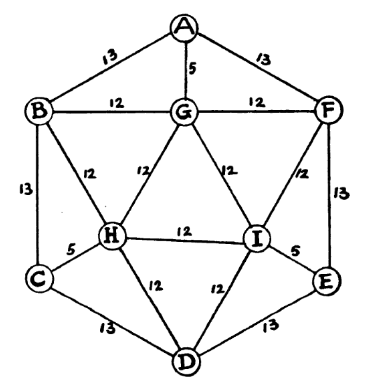
\includegraphics[width=2in]{quiz11/path-with-repetitions.png}}
\caption{\label{fig:path-with-repetitions} Path with repetitions}
\end{figure}

Write an integer \textendash{} the length of the shortest route.

{\em Note.} This graph obviously has no Euler path (since there
are more than $2$ vertices with odd degrees). The problem is to 
find a path that is likely {\bf not} simple 
(uses the same edge several times), 
but that includes every edge shown and the total of weights is minimal. 





\vspace{10pt}
{\bf Question 11}\\
Somebody placed $24$ chess rooks on a $8 \times 8$ chessboard as shown in Figure~\ref{fig:rooks}
(each horizontal and each vertical has exactly $3$ rooks). 


\begin{figure}[!htb]
\center{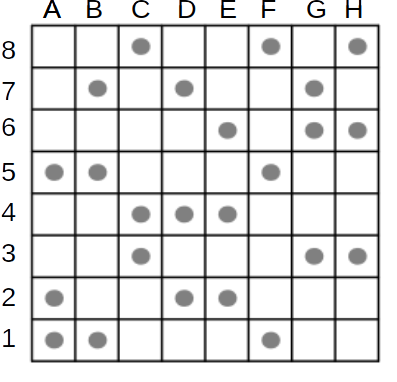
\includegraphics[width=1.5in]{quiz11/rooks.png}}
\caption{\label{fig:rooks} Path with repetitions}
\end{figure}

We imagine that this chess-board defines a bipartite graph between the  
set of all verticals $X= \{ A,B,C,D,E,F,G,H \}$ and the set of all 
horizontals $Y= \{ 1,2,3,4,5,6,7,8 \}$. Any rook defines an edge between these two sets. 
For example, the rook $C8$ defines an edge $(C,8)$. 

Find a subset of verticals $V \subseteq X$ such that $|V|=3$, but
the neighbor set has size $|N(V)| = 5$.

Write $3$ comma-separated letters in your answer (the vertices from $V$). It is 
sufficient to write just one possible answer, if there are many.

\vspace{10pt}
{\em Note 1.} For example, the answer $\textcolor{blue}{\mathtt{F,G,H}}$ does not work, 
since the set of vertices $\{ \mathtt{F},\mathtt{G},\mathtt{H} \} \subseteq X$ 
is neighboring with a set of six vertices
$\{ 1,3,5,6,7,8 \} \subseteq Y$, i.e. the rooks on these three verticals
attack six horizontals, but not five.

{\em Note 2.} For the condition of the Hall's marriage theorem we need the inequality $|V| \leq |N(V)|$ 
for {\bf every} $V \subseteq X$. You could prove to yourself that it is always satisfied
(also for all the other placements of $24$ rooks where each horizontal and each 
vertical has $3$ rooks).\\
{\em Note 3.} Interpret for yourself what does a ``perfect matching'' between the sets
$X$ and $Y$ mean in this subject-area with a chessboard and rooks.




\newpage

\subsection{Answers}


\vspace{4pt}
{\bf Question 1} Answer: $15,75$\\
Since $144 = 2^4 \cdot 3^2$, number $144$ has $(4+1)(2+1) = 15$ divisors
(the number of ways to pick powers $2^a \cdot 3^b$). 
Their Hasse diagram is shown in Figure~\ref{fig:divisibility-144-graph}
(transitive closure has many more arrows that are not shown). 

For each vertex $d_1$ we calculate the number of other vertices that
are divisible by $d_1$ (i.e. can be reached by following one or more arrows in the
Hasse diagram). Adding all those numbers gives the number of edges.

\begin{figure}[!htb]
\center{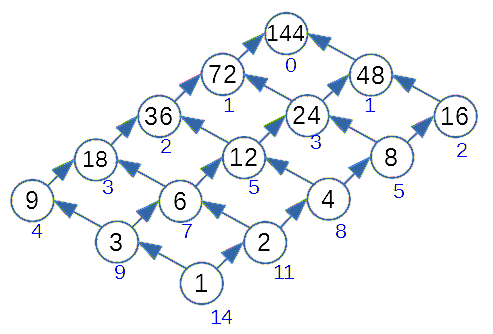
\includegraphics[width=3in]{divisibility-144-graph.png}}
\caption{\label{fig:divisibility-144-graph} Divisibility Hasse diagram.}
\end{figure}




\vspace{10pt}
{\bf Question 2} Answer: $30$\\
All the vertices on the regular $20$-gon have degree equal to $3$. 
This means that we have to drop at least $10$ edges before we 
get a simple path (because any simple path adds only even number to the degree
of any vertex in a graph). Initially $W_{20}$ has $20 + 20 = 40$ edges. 
After deleting $10$ edges (every other edge on the perimeter of the $20$-gon), 
we are left with $30$ edges.


\vspace{10pt}
{\bf Question 3} Answer: $32$\\
$60$ vertices (having degree $3$ each would create the sum of all degrees equal to $60 \cdot 3 = 180$. 
The number of edges equals one half of that; so $|E| = 90$. The number of regions
can be computed using Euler's formula: $|V| - |E| + |R| = 2$ (in our case 
$60 - 90 + |R| = 2$; therefore $|R| = 32$. 

One example of such graph is {\em truncated icosahedron}, see \url{https://bit.ly/2WaSW6I}, 
but there may be many others that are not isomorphic to it. Still, all of them 
would have the same number of regions due to Euler's formula.

\vspace{10pt}
{\bf Question 4} Answer: {\tt 9,17,10}\\
Number of vertices equals the size of the matrix $9 \times 9$, 
so $|V| = 9$. The number of edges is one half of all the $1$s written 
in the adjacency matrix; therefore $|E| = 17$. Since we can assume
that the graph $G$ is planar, it satisfies Euler's formula:
$$|V| - |E| + |R| = 2.$$
Therefore the number of regions $|R| = 10$. 

Graph (shown without edge intersections as a planar graph) is visible 
on Figure~\ref{fig:question4-graph}. In this picture we can simply count 
vertices, edges and regions. But it is usually time-consuming to 
create such pictures (and to verify that they match the adjacency matrix).

\begin{figure}[!htb]
\center{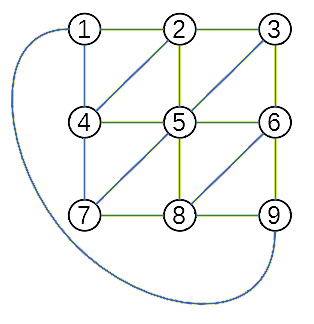
\includegraphics[width=1.5in]{quiz11/question4-graph.png}}
\caption{\label{fig:question4-graph} A planar graph}
\end{figure}


\vspace{10pt}
{\bf Question 5} Answer: $34$\\
It is easy to build a path that visits all rooms except one. 
There cannot be a circular path with exactly $35$ steps \textendash{}
one can use checkerboard pattern (color all cells in black and white). 
Every step switches the color to the opposite; after exactly $35$ color switches
the color would be opposite \textendash{} the path cannot return back to cell $A$.


\vspace{10pt}
{\bf Question 6} Answer: $72$\\
We know that the sum of two sizes $|X| + |Y| = 17$, 
and the maximum number of edges is $|X| \cdot |Y|$. 
The greatest possible product of two numbers is
when they are closest to each other: 
$8 \cdot 9 = 72$. (We can try out all combinations of two numbers
that add up to $17$ to see that this is the largest one.)

We can write the following algebraic inequalities: 
$$|X| \cdot |Y| \leq \left( \frac{|X| + |Y|}{2} \right)^2,$$
$$4 |X| \cdot |Y| \leq \left( |X| + |Y| \right)^2,$$
$$4 |X| \cdot |Y| \leq |X|^2 + |Y|^2 + 2 |X| \cdot |Y|,$$
$$0 \leq |X|^2 + |Y|^2 = 2 |X| \cdot |Y| = (|X| + |Y|)^2.$$

From the first inequality we imply that $|X| \cdot |Y| \leq (17/2)^2 = 72.25$. 
Since the number of edges cannot be fractional, $72$ is indeed the largest number.



\vspace{10pt}
{\bf Question 7} Answer: {\tt FTT}\\
{\bf (A)} False. No cubic graph can have odd number of vertices 
(the sum of all degrees of all vertices should be even \textendash{} twice the number of edges).\\
{\bf (B)} True. $K_{3,3}$ is bipartite graph (it does not contain any ``triangles'': three vertices
that are all mutually connected). But the graph on Figure~\ref{fig:cubic-graph-6}
is not bipartite (so it is not isomorphic
to $K_{3,3}$.

\begin{figure}[!htb]
\center{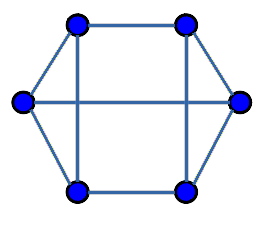
\includegraphics[width=1in]{quiz11/cubic-graph-6.png}}
\caption{\label{fig:cubic-graph-6} Cubic graph with 6 vertices.}
\end{figure}

{\bf (C)} True. You can draw a regular octagon and add all the long diagonals. 
Now every vertex is adjacent with three vertices (both neighbors and the opposite one). 


\vspace{10pt}
{\bf Question 8} Answer: {\tt FFT}\\
{\bf (A)} False. In a simple directed graph with $5$ vertices, an indegree 
$5$ means that all vertices should point arrows to the given vertex (including the vertex itself). 
But in this case there cannot be any vertices with outdegree $0$.\\
{\bf (B)} False. A graph with $8$ vertices of degree $3$ means that it has $\frac{8 \cdot 3}{2} = 12$ edges. 
According to Euler's formula, the number of regions should be $R = 2 + E - V = 6$. Therefore 
such a graph should have $6$ (not $5$) regions.\\
{\bf (C)} True. Such graph exists. For example Octahedron - see \url{https://bit.ly/3f1gnrG}.



\vspace{10pt}
{\bf Question 9} Answer: {\tt 8,9,5,7}

{\footnotesize
\begin{tabular}{|l|l|l|} \hline
Set $S$ & Weights of $\overline{S}$ & Added to $S$ \\ \hline
$\{ s \}$ & $w(t,x,y,z) = (10,\infty,5,\infty)$ & $y$ (min path $5$) \\  \hline
$\{ s,y \}$ & $w(t,x,z) = (8,\infty,7)$ & $z$ (min path $7$) \\ \hline
$\{ s,y,z \}$ & $w(t,x) = (8,9)$ & $t$ (min path $8$) \\ \hline
$\{ s,t,y,z \}$ & $w(x) = 9$ & $x$ (min path $9$) \\ \hline
\end{tabular}
}


\vspace{10pt}
{\bf Question 10} Answer: {\tt 211}\\
There are altogether $6$ vertices with odd degrees (one of them is $A$). If we start our travel in $A$
and end it in any other vertex with odd degree (say, in $G$), then there are 
four more vertices with odd degrees. By adding edges $(C,H)$ and $(I,E)$ two times, we can 
build the required path (each of these edges has weight $5$). Therefore the full length of the 
path is the sum of all weights: 
$$3 \cdot (12 + 12 + 12) + 3 \cdot (13 + 13 + 5) + (5 + 5).$$

\begin{figure}[!htb]
\center{
\includegraphics[width=1.5in]{quiz11/path-with-repetitions2.png}}
\caption{\label{fig:path-with-repetitions2} Path with Repetitions (Solved).}
\end{figure}


\vspace{10pt}
{\bf Question 11} Answer: {\tt "A,B,D"}, {\tt "A,B,F"}, 
{\tt "C,E,H"}, {\tt "C,G,H"}, {\tt "D,E,G"}\\
There are five ways to select the verticals (any one of them is correct). 
Since the rooks (as edges linking horizontals with verticals) satisfy the Hall's Marriage theorem, 
there exists a perfect matching: One can select $8$ rooks (out of the $24$) so that
each rook has its own horizontal and its own vertical. In other words, they do not attack each other. 

We can start searching this perfect matching using ``backtracking'' \textendash{} first 
try to pick the minimum possible horizontal in each vertical (avoiding any attacking position). 
If this leads in a dead end, then start moving the rooks that have been placed last. 
This very quickly leads to a solution (Figure~\ref{fig:rooks2}). There are also many other 
perfect matchings.

\begin{figure}[!htb]
\center{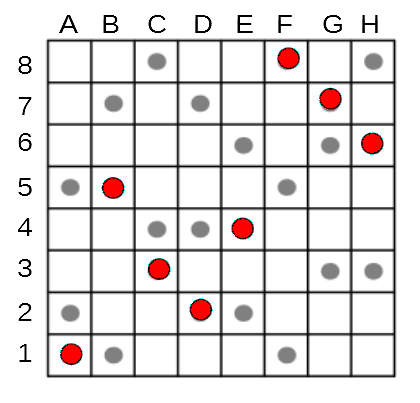
\includegraphics[width=1.5in]{quiz11/rooks2.png}}
\caption{\label{fig:rooks2} 8 selected rooks shown red}
\end{figure}




\end{document}




\newpage
\documentclass[jou]{apa6}

\usepackage[american]{babel}

\usepackage{csquotes}
\usepackage[style=apa,sortcites=true,sorting=nyt,backend=biber]{biblatex}
\DeclareLanguageMapping{american}{american-apa}
\addbibresource{bibliography.bib}


%%%%%%%%%%%%%%%%%%%%%%%%%%%%%%%%%%%%%%%%
%% Discrete Structures
%% The start of RBS stuff
%%%%%%%%%%%%%%%%%%%%%%%%%%%%%%%%%%%%%%%%

% Working internal and external links in PDF
\usepackage{hyperref}
% Extra math symbols in LaTeX
\usepackage{amsmath}
\usepackage{gensymb}
\usepackage{amssymb}
% Enumerations with (a), (b), etc.
\usepackage{enumerate}

\let\OLDitemize\itemize
\renewcommand\itemize{\OLDitemize\addtolength{\itemsep}{-6pt}}

\usepackage{etoolbox}
\makeatletter
\preto{\@verbatim}{\topsep=3pt \partopsep=3pt }
\makeatother

% These sizes redefine APA for A4 paper size
\oddsidemargin 0.0in
\evensidemargin 0.0in
\textwidth 6.27in
\headheight 1.0in
\topmargin -24pt
\headheight 12pt
\headsep 12pt
\textheight 9.19in



\title{Sample Quiz 8}
\author{Discrete Structures, Spring 2020}
\affiliation{RBS}

\leftheader{Discrete Sample Quiz 8}

\abstract{%
}

%\keywords{}

\setlength\parindent{0pt}

\begin{document}

%\thispagestyle{empty}

\twocolumn
\section{Worksheet 12: Trees}

{\bf Question 1.} Count the objects:\\
{\bf (A)} If $T$ is a tree with $999$ vertices, then $T$ has $\ldots$ edges.\\
{\bf (B)} There are $\ldots$ non-isomorphic trees with four vertices.\\
{\bf (C)} There are $\ldots$ non-isomorphic rooted trees with four vertices (isomorphism 
for rooted trees can change map any node to any other; but it should map root to root).\\
{\bf (D)} There are $\ldots$ full binary trees with six vertices.\\
{\bf (E)} The cycle graph $C_7$ has $\ldots$ spanning trees.\\
{\bf (F)} If $T$ is a binary tree with 100 vertices, its minimum height is $\ldots$.\\
{\bf (G)} If $T$ is a full binary tree with $101$ vertices, its minimum height is $\ldots$.\\
{\bf (H)} If $T$ is a full binary tree with $101$ vertices, its maximum height is $\ldots$.\\
{\bf (I)} If $T$ is a full binary tree with $50$ leaves, its minimum height is $\ldots$.\\
{\bf (J)} Every full binary tree with $61$ vertices has $\ldots$ leaves.\\
{\bf (K)} Every full binary tree with $50$ leaves has $\ldots$ vertices.\\
{\bf (L)} Every 3-ary tree with 13 vertices has $\ldots$ leaves.

\vspace{10pt}
{\bf Question 2.} Find, if a statement is true or false:\\
{\bf (A)} If T is a tree with 17 vertices, then there is a simple path in T of length 17.\\
{\bf (B)} Every tree is bipartite.\\
{\bf (C)} There is a tree with degrees $3, 2, 2, 2, 1, 1, 1, 1, 1$.\\
{\bf (D)} There is a tree with degrees $3, 3, 2, 2, 1, 1, 1, 1$.\\
{\bf (E)} If two trees have the same number of vertices and the same degrees, then the two trees are isomorphic.\\
{\bf (F)} If $T$ is a tree with $50$ vertices, the largest degree that any vertex can have is $49$.\\
{\bf (G)} In a binary tree with $16$ vertices, there must be a path of length $4$.\\
{\bf (H)} If $T$ is a rooted binary tree of height $5$, then $T$ has at most $25$ leaves.


\vspace{10pt}
{\bf Question 3.}\\
Suppose you have $50$ coins, one of which is counterfeit 
(either heavier or lighter than the others). You use a
balance scale to find the bad coin. Prove that $4$ weighings 
are not enough to guarantee that you find the
bad coin and determine whether 
it is heavier or lighter than the other coins.


\vspace{10pt}
{\bf Question 4.}\\
Suppose you have $5$ coins, one of which is counterfeit 
(either heavier or lighter than the other four). You use
a pan balance scale to find the bad coin and determine 
whether it is heavier or lighter.\\
{\bf (A)} Prove that $2$ weighings are not enough to guarantee 
that you find the bad coin and determine whether it
is heavier or lighter.\\
{\bf (B)}  Draw a decision tree for weighing the coins to determine 
the bad coin (and whether it is heavier or lighter)
in the minimum number of weighings.


\vspace{10pt}
{\bf Question 5.}\\
Suppose you have $5$ coins, one of which is heavier than the other four. 
Draw the decision tree for using a
balance scale to find the heavy coin. How many weighings would you need?



\vspace{10pt}
{\bf Question 6.} 
\begin{figure}[!htb]
\center{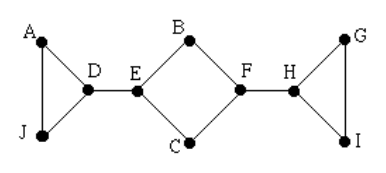
\includegraphics[width=2.5in]{quiz-sample-12/quiz12-graph.png}}
\caption{\label{fig:quiz12-graph} Graph for DFS and BFS traversal.}
\end{figure}


{\bf (A)} Using alphabetical ordering, find a spanning tree for the graph on Figure~\ref{fig:quiz12-graph} by using a depth-first search.\\
{\bf (B)} Using alphabetical ordering, find a spanning tree for this graph by using a breadth-first search.\\
{\bf (C)} Using the ordering $C, D, E, F, G, H, I, J, A, B$, find a spanning tree for this graph by using a depth-first search.\\
{\bf (D)} Using the ordering $C, D, E, F, G, H, I, J, A, B$, find a spanning tree for this graph by using a breadth-first search.\\
{\bf (E)} Using reverse alphabetical ordering, find a spanning tree for the graph by using a depth-first search.\\
{\bf (F)} Using reverse alphabetical ordering, find a spanning tree for the graph by using a breadth-first search.






\vspace{10pt}
{\bf Question 7.}\\
Write the compound proposition $(\neg p) \rightarrow (q \vee (r \wedge \neg s))$ 
as the abstract syntax tree ($\neg$, $\rightarrow$, $\vee$ and $\wedge$ operators
are inner nodes; but $p,q,r,s$ are leaves).\\
List the graph nodes in pre-order, in-order and post-order traversal of this syntax tree.


\vspace{10pt}
{\bf Question 8.}\\
Draw the abstract syntax tree, the preorder and postorder traversal 
of $(8x - y)^5 - 7\sqrt{4z - 3}$.


\vspace{10pt}
{\bf Question 9.} 
The string\\
$p\;r\;q\;\rightarrow\;\neg\;q\;\triangle\;p\;\rightarrow\;\wedge$\\
is postfix notation for a logic expression; however, there is a misprint. The
triangle should be one of these three: $r$, $\vee$, or $\neg$. 
Determine which of these three it must be and explain your
reasoning.


\mbox{}
\newpage
\subsection{Answers}

\vspace{10pt}
{\bf Question 1.} Answer:\\
{\bf (A)} If $T$ is a tree with $999$ vertices, then $T$ has $998$ edges.\\
{\bf (B)} There are $2$ non-isomorphic trees with four vertices.\\
{\bf (C)} There are $4$ non-isomorphic rooted trees with four vertices.\\
{\bf (D)} There are $0$ full binary trees with six vertices.\\
{\bf (E)} The cycle graph $C_7$ has $7$ spanning trees.\\
{\bf (F)} If $T$ is a binary tree with 100 vertices, its minimum height is $6$.\\
{\bf (G)} If $T$ is a full binary tree with $101$ vertices, its minimum height is $6$.\\
{\bf (H)} If $T$ is a full binary tree with $101$ vertices, its maximum height is $50$.\\
{\bf (I)} If $T$ is a full binary tree with $50$ leaves, its minimum height is $6$.\\
{\bf (J)} Every full binary tree with $61$ vertices has $31$ leaves.\\
{\bf (K)} Every full binary tree with $50$ leaves has $99$ vertices.\\
{\bf (L)} Every 3-ary tree with 13 vertices has $9$ leaves.

\vspace{10pt}
{\bf Question 2.} Answer: TBD \\

\vspace{10pt}
{\bf Question 3.} Answer:\\

Four weighings could give at most $3^4 = 81$ outcomes (each time we use scales there are
three possible results). But the problem has $2 \cdot 50$ different situations
(any of the $50$ coins can be different; and it can be either heavier or lighter). 

\vspace{10pt}
{\bf Question 4.} Answer: TBD \\

\vspace{10pt}
{\bf Question 5.} Answer: TBD \\

\vspace{10pt}
{\bf Question 6.} Answer: TBD \\

\vspace{10pt}
{\bf Question 7.} Answer: TBD \\

\vspace{10pt}
{\bf Question 8.} Answer: TBD \\

\vspace{10pt}
{\bf Question 9.} Answer: TBD \\






\end{document}



\newpage
\documentclass[jou]{apa6}

\usepackage[american]{babel}

\usepackage{csquotes}
\usepackage[style=apa,sortcites=true,sorting=nyt,backend=biber]{biblatex}
\DeclareLanguageMapping{american}{american-apa}
\addbibresource{bibliography.bib}


%%%%%%%%%%%%%%%%%%%%%%%%%%%%%%%%%%%%%%%%
%% Discrete Structures
%% The start of RBS stuff
%%%%%%%%%%%%%%%%%%%%%%%%%%%%%%%%%%%%%%%%

% Working internal and external links in PDF
\usepackage{hyperref}
% Extra math symbols in LaTeX
\usepackage{amsmath}
\usepackage{gensymb}
\usepackage{amssymb}
% Enumerations with (a), (b), etc.
\usepackage{enumerate}
\usepackage[framemethod=TikZ]{mdframed}
\usepackage{xcolor}

\let\OLDitemize\itemize
\renewcommand\itemize{\OLDitemize\addtolength{\itemsep}{-6pt}}

\usepackage{etoolbox}
\makeatletter
\preto{\@verbatim}{\topsep=3pt \partopsep=3pt }
\makeatother

% These sizes redefine APA for A4 paper size
\oddsidemargin 0.0in
\evensidemargin 0.0in
\textwidth 6.27in
\headheight 1.0in
\topmargin -24pt
\headheight 12pt
\headsep 12pt
\textheight 9.19in



\title{Sample Quiz 8}
\author{Discrete Structures, Spring 2020}
\affiliation{RBS}

\leftheader{Discrete Sample Quiz 8}

\abstract{%
}

%\keywords{}

\setlength\parindent{0pt}

\begin{document}

%\thispagestyle{empty}

\twocolumn
\section{Quiz 12: Trees}

{\bf Question 1.} The wheel graph $W_4$ has $5$ vertices: 
$4$ vertices form a cycle graph $C_4$ \textendash{} a square; 
one more vertex sits in the middle and is connected with the remaining $4$ vertices. 
($W_4$ is isomorphic to an ordinary Egyptian pyramid.) 
Assume that all vertices in the wheel graph are named with letters and are distinguishable. 
Find the number of unrooted spanning trees in the $W_4$.\\
Write a positive integer in your answer.

\vspace{10pt}
{\bf Question 2.} It is known that a full $m$-ary tree $T$ has $25$ leaves, but the parameter $m$ is 
not known \textendash{} it can take any fixed value: $m = 2,3,4,\ldots$. 
How many inner nodes can $T$ have? Find all possible answers.\\
Write an increasing comma-separated list.

\vspace{10pt}
{\bf Question 3.}\\ There is a rooted tree with $111$ vertices and each vertex can have up to $3$ children. 
Find the minimum and the maximum height of this tree.\\
Write two comma-separated integers.


\vspace{10pt}
{\bf Question 4.}\\ 
Assume that there is a rooted tree (with anonymous/unnamed vertices and unordered children) and its vertices have 
the following degrees $3, 3, 2, 2, 1, 1, 1, 1$. It is also known that its root vertex has $3$ children. 
Find the number of such rooted unordered trees.\\
Write a positive integer.


\vspace{10pt}
{\bf Question 5.}

\begin{figure}[!htb]
\center{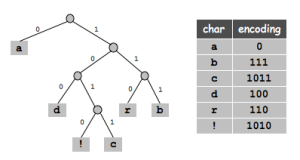
\includegraphics[width=3.2in]{quiz12/huffman-tree.png}}
\caption{\label{fig:huffman-tree} Encoding with a Tree.}
\end{figure}

Figure~\ref{fig:huffman-tree} shows an efficient method to send messages
(like {\tt abracadabra!}) using $6$ characters.
Assume that the characters appear with the following probabilities:\\
{\small
\begin{tabular}{|l|c|c|c|c|c|c|} \hline
Symbol & {\tt a} & {\tt b} & {\tt d} & {\tt r} & {\tt c} & {\tt !} \\ \hline
Probability &  $1/2$ & $1/8$ & $1/8$ & $1/8$ & $1/16$ & $1/16$ \\ \hline
\end{tabular}\\
}
Find the expected number of bits used per character (i.e. $E(X)$ \textendash{} the expected value of
the random variable $X$, which describes the number of bits used per one
character from this random distribution.)\\
Write a real number \textendash{} the number of bits rounded to the nearest thousandth.

%{\em Note.} For the given probabilities, this tree offers the best compression
%(using it for the encoding needs the smallest 
%expected number of bits). For such optimal codes we say that the expected number of bits
%for sending one character equals the {\em entropy} of the probability distribution.
%It is fine, if the entropy is a fractional (non-integer) number of bits.



 
 


\vspace{10pt}
{\bf Question 6.} 
The string
$$\rightarrow\;\rightarrow\;\rightarrow\;\rightarrow\;\rightarrow\;a\;b\;\textcolor{red}{\triangle}\;\neg\;c\;\neg\;d\;c\;e\;\rightarrow\;\neg\;a\;\rightarrow\;d\;e.$$
is the prefix notation for a Boolean logic expression with one symbol replaced by a $\textcolor{red}{\triangle}$. 
What can this $\textcolor{red}{\triangle}$ represent?\\
{\bf (A)} It is a propositional variable ($a,b,c$ or similar).\\
{\bf (B)} It is a unary Boolean operator ($\neg$ or similar).\\
{\bf (C)} It is a binary Boolean operator ($\rightarrow$ or similar).\\
{\bf (D)} It cannot be any of these; the expression is invalid in all these cases.

Write the answer letter (A, B, C, or D).



\vspace{10pt}
{\bf Question 7.} 
Imagine that you search for all ways how to place $4$ queens on a $4 \times 4$ chessboard so that 
they do not attack each other. (A chess queen attacks all squares on its horizontal, on its vertical
and also on both diagonals.)\\
Imagine that you build a tree for this:\\
{\bf (Level 0 to Level 1)} The root of the tree is an empty $4 \times 4$ chess-board; you add to it four children 
(all $4$ ways how you can place a queen on the 1st row of the chess-board).\\
{\bf (Level 1 to Level 2)} For any of the vertices you added in the previous step, add children on level $2$ by placing 
another queen on the 2nd row so that it does not attack the first one.\\
In general, the vertex on level $L=i$ has queens on rows $1,\ldots,i$ that do not attack each other. 
Any vertex on level $L=4$ will be a solution to this ``4 queens problem'' with all four rows containing a queen.

Write the total number of vertices in this tree (that the backtracking algorithm will visit).


\vspace{10pt}
{\bf Question 8.} An undirected graph $G = (V,E)$ has the set of vertices $V$ \textendash{} 
the set of all positive divisors of the number $900$ (including $1$ and $900$ itself).
A pair of divisors $(d_1,d_2)$ is an edge in $G$ iff their ratio
$d_1/d_2$ (or $d_2/d_1$) is a prime number.

In the root vertex $v_1=1$ we start the BFS (Breadth-first-search) traversal of the graph $G$. For every vertex 
we visit all its adjacent vertices in increasing order (for example edges $(1,2)$, $(1,3)$ and $(1,5)$ 
are visited in this order. When all the children of vertex $1$ are visited, 
we start visiting all the adjacent vertices of $v_2=2$, and so on.). We get the BFS traversal order like this:
$$v_1=1,\,v_2=2,\,v_3=3,\,v_4=5,\,v_5=4,\,\ldots$$
Find the vertices $v_{13},\,v_{14},\,v_{15}$ in this BFS order.

Write three comma-separated numbers.

%\newpage
\vspace{10pt}
{\bf Question 9.}

\begin{figure}[!htb]
\center{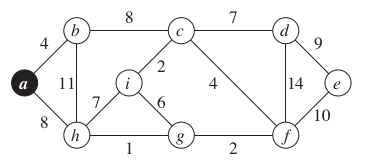
\includegraphics[width=2in]{quiz12/prim-algorithm.png}}
\caption{\label{fig:prim-algorithm} Weighted Graph.}
\end{figure}


Find the weight of a minumum spanning tree (MST) in the tree shown in Figure~\ref{fig:prim-algorithm}. 
In order to construct this tree, you can use Prim's algorithm (Rosen2019, p.836). 
Start in vertex $a$ - this is your first tree $T_1$. 
In every step pick the minimum weight edge that is adjacent to $T_i$ (and does 
not create any loop) \textendash{} add it to the tree $T_i$, and obtain the next 
tree $T_{i+1}$. Continue adding the minimum weight edges until all vertices are connected.
(In the second step you will have a choice 
to add $(b,c)$ or $(a,h)$ as both edges have the same weight $8$. There may be several MSTs
in a graph, but all of them will have the same total weight.)

Write the total MST weight as a number.


\vspace{10pt}
{\bf Question 10.}
The vertices in the directed graph (Figure~\ref{fig:dfs-traversal2}) are visited in the DFS
order. You start with the alphabetically smallest vertex ($q$), order all the vertices connected to it
alphabetically, then build the DFS traversal. 

\begin{figure}[!htb]
\center{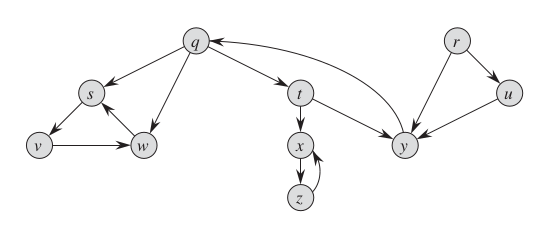
\includegraphics[width=3in]{quiz12/dfs-traversal2.png}}
\caption{\label{fig:dfs-traversal2} Graph for DFS traversal.}
\end{figure}




Write the sequence with parentheses and vertices for the graph 
on Figure 3 \textendash{} similar to the sequence (\ref{eq:dfs-search-order}) \textendash{} see Appendix. 
Each of its $10$ vertices should be mentioned in your 
traversal order twice (the first time with an opening parenthesis, the second time 
with a closing parenthesis).




\mbox{}
\newpage

{\bf Appendix: DFS}

\begin{figure}[!htb]
\center{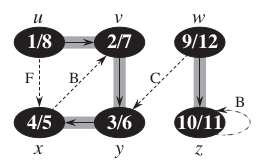
\includegraphics[width=1.4in]{quiz12/dfs-traversal.png}}
\caption{\label{fig:dfs-traversal} Sample DFS traversal.}
\end{figure}

Figure~\ref{fig:dfs-traversal} shows a DFS (Depth-First-Search) traversal
in a directed graph. Vertexes are visited in alphabetical order 
(so $u$ is visited first; followed by its alphabetically first 
child $v$, followed by $y$, followed by $x$. After that
we visit another tree (unreachable from the first one) \textendash{}
$w$ followed by $z$.)\\
{\bf Tree edges} that belong to the DFS traversal tree are shaded;\\
{\bf Back edges} that point back from a vertex to its ancestor in the tree (or a loop to itself)
are labeled by $B$;\\
{\bf Forward edges} that jump from a vertex to its descendant in the DFS tree (other than a child) are
labeled by $F$;\\
{\bf Cross edges} that jump between two vertices that are not descendants/ancestors of 
each other are labeled by $C$.

The following sequence
\begin{equation} \label{eq:dfs-search-order}
\textcolor{blue}{\mathtt{(u\;(v\;(y\;(x\;x)\;y)\;v)\;u)\;(w\;(z\;z)\;w)}}
\end{equation}
denotes the DFS traversal order in the oriented graph. 
Every time when we enter some vertex (and its subtree), 
we open a parenthesis and write the vertex name; when we leave, 
we write the vertex name again and close the parenthesis.\\
This order is also written inside each vertex (for example {\tt 1/8} 
for vertex $u$ means that we entered it in Step 1, and left it in 
Step 8). For vertex $z$ this pair is {\tt 10/11} (we entered this leaf
of the DFS tree and immediately left it).
%\end{mdframed}


%\begin{mdframed}[roundcorner=6pt]
%\section{Appendix 2: Prim's Algorithm}

%\end{mdframed}

\newpage
\subsection{Answers}

\vspace{4pt}
{\bf Question 1.} Answer: {\tt 45} \\

There are only three kinds of trees with $5$ vertices, if isomorphic trees count as the same. 
See {\em isomers of pentane} \textendash{} \url{https://bit.ly/2W4BWiw} (either the vertex degrees are 
$1,2,2,2,1$, or $1,2,3,1,1$, or $4,1,1,1,1$).

Let us denote the vertices by $A,B,C,D,E$ ($E$ being the vertex at the top of the pyramid). 
The only non-existing edges are $(A,C)$ and $(B,D)$ (otherwise it is almost like $K_5$). 
In Figures~\ref{fig:spanning-trees-on-w5-a}, \ref{fig:spanning-trees-on-w5-b}, 
\ref{fig:spanning-trees-on-w5-c} we show different subcases depending 

\begin{figure}[!htb]
\center{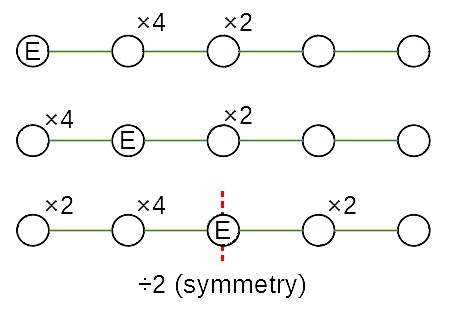
\includegraphics[width=2.2in]{quiz12/spanning-trees-on-w5-a.png}}
\caption{\label{fig:spanning-trees-on-w5-a} 24 trees with all degrees $\leq 2$.}
\end{figure}

\begin{figure}[!htb]
\center{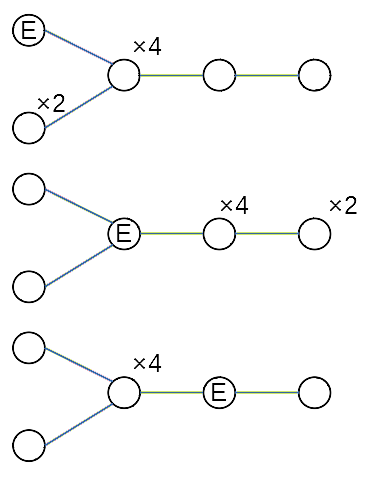
\includegraphics[width=1.8in]{quiz12/spanning-trees-on-w5-b.png}}
\caption{\label{fig:spanning-trees-on-w5-b} 20 trees with one degree $=3$.}
\end{figure}

\begin{figure}[!htb]
\center{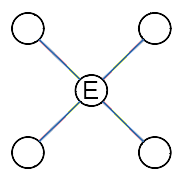
\includegraphics[width=0.9in]{quiz12/spanning-trees-on-w5-c.png}}
\caption{\label{fig:spanning-trees-on-w5-c} 1 tree with one degree $=4$.}
\end{figure}

$$N = (8 + 8 + 8) + (8 + 8 + 4) + (1) = 45.$$


\vspace{4pt}
{\bf Question 2.} Answer: {\tt 1,2,3,4,6,8,12,24} \\
In a full $m$-ary tree initially there is just one 
node (it is the root and also a leaf). After that
the number of leaves can increase by $m-1$ in a single step 
(one leaf becomes an internal node and creates exactly $m$ children). 
The question now becomes \textendash{} in how many arithmetic
progressions both numbers $1$ and $25$ participate. 
We get these variants:

$$\left\{ \begin{array}{l}
1,2,3,\ldots,25 \\
1,3,5,7,9,11,13,15,17,19,21,23,25 \\
1,4,7,10,13,16,19,22,25 \\
1,5,9,13,17,21,25 \\
1,7,13,19,25 \\
1,9,17,25 \\
1,13,25 \\
1,25 \\
\end{array} \right.$$

In each variant we count the number of increments
(how many times $m-1$ was added in order to get $25$). At every such step 
an inner node is created.
The number of inner nodes can be computed as $\frac{25-1}{m-1}$. 

\begin{tabular}{|l|l|} \hline
$m$ & Inner nodes \\ \hline
$2$ & $24$ \\ \hline
$3$ & $12$ \\ \hline
$4$ & $8$ \\ \hline
$5$ & $6$ \\ \hline
$7$ & $4$ \\ \hline
$9$ & $3$ \\ \hline
$13$ & $2$ \\ \hline
$25$ & $1$ \\ \hline
\end{tabular}





\vspace{4pt}
{\bf Question 3.} Answer: {\tt 4,110}

{\bf Minimum height.} There is one vertex (the root) at depth $d=0$, 
at most $3$ vertices at $d=1$, at most $9$ vertices at $d=2$, 
at most $27$ vertices at $d=3$ and at most $81$ vertices at $d=4$. 
If maximum depth is $4$ (i.e. the height of the tree is also $4$), then 
there can be at most $1 + 3 + 9 + 27 + 81 = 121$
vertices in the tree. Which is just fine, since $111 < 121$. 

{\bf Maximum height.} In this case each vertex has just one child. 
The deepest node has depth $d=110$ (one less than the number of nodes
in the tree). 


\vspace{4pt}
{\bf Question 4.} Answer: {\tt 6}

We can sort cases depending on the location of the other vertex $v_1$
with degree $3$ (it is known that another one is root; let us denote the root by $v_0$).
That other vertex can have depth $1$, $2$ or $3$.  

{\bf Case 1.} $\text{depth}(v_1) = 1$. There are three possible trees in this case; 
the two vertices of degree $2$ can be either both children of $v_0$, or both of $v_1$, 
or one can be a child of $v_1$, and another of $v_0$.\\
{\bf Case 2.}  $\text{depth}(v_1) = 2$. There are two possible trees in this case; 
one of the vertices of degree $2$ is beteween $v_0$ and $v_1$; but another vertex
of degree $2$ can be a child of $v_0$, or a child of $v_1$.\\
{\bf Case 3.} $\text{depth}(v_1) = 3$. There is just one tree in this case. 
Both vertices of degree $2$ are between $v_0$ and $v_1$. 






\vspace{4pt}
{\bf Question 5.} Answer: {\tt 2.125} \\
To geet the expected value of the random variable (the length of the code in bits)
multiply the respective code lengths for all six letters of the alphabet
by their respective probabilities: 

$$1 \cdot \frac{1}{2} + 3 \cdot \frac{1}{8} + 3 \cdot \frac{1}{8} + 3 \cdot \frac{1}{8} + 4 \cdot \frac{1}{16} + 4 \cdot \frac{1}{16} = 2\frac{1}{8}.$$

{\em Note.} Variable length codes where one code is never a prefix of another and
all the codes can be arranged in a binary tree, where grouping them starts by the two least frequent letters
({\tt !} and {\tt c} in our case) is named {\em Huffman tree}. 

\vspace{4pt}
{\bf Question 6.} Answer: {\tt C}\\
In any (infix, prefix or postfix) expression the number of binary operators (in our case the only 
such operator is $\rightarrow$) should be one less than the number of operands (in our case 
these are the Boolean variables $a$,$b$,$c$,$d$,$e$). Unary operators (in our case $\neg$) do not count. 

In our expression so far there are $7$ operators $\rightarrow$. There are also $9$ Boolean variables. 
Therefore the triangle should become a binary operator $\rightarrow$. 
The expression looks like this: 
$$\rightarrow\;\rightarrow\;\rightarrow\;\rightarrow\;\rightarrow\;a\;b\;\textcolor{red}{\rightarrow}\;\neg\;c\;\neg\;d\;c\;e\;\rightarrow\;\neg\;a\;\rightarrow\;d\;e.$$

Here is the regular (infix) representation of the same Boolean expression:

{\footnotesize
$$((((a \rightarrow b) \rightarrow (\neg c \textcolor{red}{\rightarrow} \neg d)) \rightarrow c) \rightarrow e) 
  \rightarrow (\neg a \rightarrow (d \rightarrow e)).$$
}

\vspace{4pt}
{\bf Question 7.} Answer: {\tt 17}\\

If we denote the rows/horizontals by numbers $1,2,3,4$ and the columns/verticals by letters $A,B,C,D$
as in ordinary chess, we can denote adding queens in the tree shown in Figure~\ref{fig:backtracking-4-queens}. 
The only two solutions are two shaded nodes at the bottom. All other placements of queens are 
dead ends. 

{\em Note.} Not pursuing these dead ends (not going deeper, if we know that it is useless) 
reduces the number of nodes to consider to $17$ (down from $4! = 24$ or even $4^4 = 256$, if we would
apply {\em brute force}). This is not very much, but for larger chess boards the savings are larger.
See \url{https://bit.ly/3aQ1feo}.

\begin{figure}[!htb]
\center{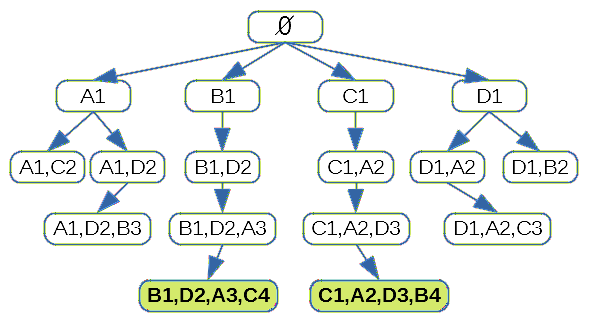
\includegraphics[width=2.4in]{quiz12/backtracking-4-queens.png}}
\caption{\label{fig:backtracking-4-queens} Backtracking tree: 4 Queens problem.}
\end{figure}


\vspace{4pt}
{\bf Question 8.} Answer: {\tt 18,30,50} \\

You can determine the order of the vertices in the BFS traversal by counting vertices
layer by layer (Figure~\ref{fig:divisors-of-900}). 
Note that the number $30 = \sqrt{900}$ is the $14$th vertex in the BFS traversal (it is in the very middle). 

\begin{figure}[!htb]
\center{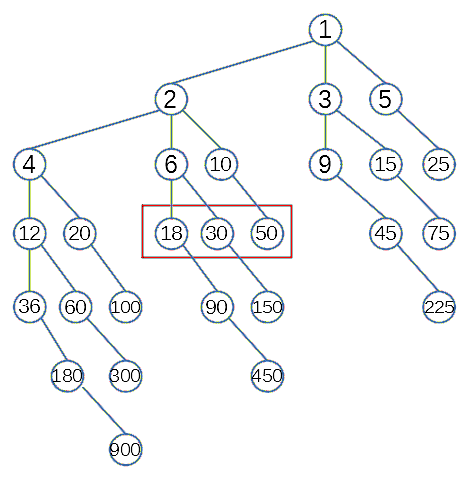
\includegraphics[width=2in]{quiz12/divisors-of-900.png}}
\caption{\label{fig:divisors-of-900} BFS tree with divisors of 900.}
\end{figure}



\vspace{4pt}
{\bf Question 9.} Answer: {\tt 37} \\

We add edges using Prim's algorithm: 

\begin{tabular}{|l|l|l|} \hline
Step 1 & $AB$ & 4 \\ \hline
Step 2 & $BC$ & 8 \\ \hline
Step 3 & $CI$ & 2 \\ \hline
Step 4 & $CF$ & 4 \\ \hline
Step 5 & $FG$ & 2 \\ \hline
Step 6 & $GH$ & 1 \\ \hline
Step 7 & $CD$ & 7 \\ \hline
Step 8 & $DE$ & 9 \\ \hline
\end{tabular}


Total weight: 

$$4 + 8 + 2 + 4 + 2 + 1 + 7 + 9 = 37.$$


\vspace{4pt}
{\bf Question 10.} Answer:\\

$$\textcolor{blue}{\mathtt{(q\,(s\,(v\,(w\;w)\,v)\,s)\,(t\,(x\,(z\;z)\,x)\,(y\,y)\,t)\,q)\;\;(r\,(u\;u)\,r)}}$$

The DFS traversal creates two trees 
with $q$ and $r$ as their roots respectively.

\end{document}




\newpage
\documentclass[jou]{apa6}

\usepackage[american]{babel}

\usepackage{csquotes}
\usepackage[style=apa,sortcites=true,sorting=nyt,backend=biber]{biblatex}
\DeclareLanguageMapping{american}{american-apa}
\addbibresource{bibliography.bib}


%%%%%%%%%%%%%%%%%%%%%%%%%%%%%%%%%%%%%%%%
%% Discrete Structures
%% The start of RBS stuff
%%%%%%%%%%%%%%%%%%%%%%%%%%%%%%%%%%%%%%%%

% Working internal and external links in PDF
\usepackage{hyperref}
% Extra math symbols in LaTeX
\usepackage{amsmath}
\usepackage{gensymb}
\usepackage{amssymb}
% Enumerations with (a), (b), etc.
\usepackage{enumerate}

\let\OLDitemize\itemize
\renewcommand\itemize{\OLDitemize\addtolength{\itemsep}{-6pt}}

\usepackage{etoolbox}
\makeatletter
\preto{\@verbatim}{\topsep=3pt \partopsep=3pt }
\makeatother

% These sizes redefine APA for A4 paper size
\oddsidemargin 0.0in
\evensidemargin 0.0in
\textwidth 6.27in
\headheight 1.0in
\topmargin -24pt
\headheight 12pt
\headsep 12pt
\textheight 9.19in



\setlength\parindent{0pt}

\title{Sample Quiz 4}
\author{Discrete Structures, Fall 2020}
\affiliation{RBS}

\leftheader{Discrete Sample Quiz 4}

\abstract{%
}

%\keywords{}

\begin{document}

%\thispagestyle{empty}

\twocolumn
\section{Midterm Preparation: Sample Problems}

{\footnotesize
Midterm may contain 3-5 computation problems \textendash{}
Part A, and also 1-2 analysis problems \textendash{} Part B and/or 
1-2 proofs (see Part C). Expect around 8 problems in the midterm (it would be 
about 15 minutes per problem). 

This document is {\bf not} a mock exam; it contains $42$ sample questions
(many more than you would expect to get in actual midterm). This material 
is meant for discussion in order to prepare and to show some variations of the 
problems.

Proofs will closely follow some pattern that has been shown in a homework 
exercise (a variant of an existing proof). 
Also the computation and analysis tasks will follow a 
recognizable pattern that is presented in this preparation material 
or any of the quizzes or homeworks.

Besides the proofs, midterm can contain
procedural problems (applying algorithms in one
particular situation); analysis tasks (for example, 
formalize something with predicates or quantifiers or apply some
other conceptual knowledge) and so on. 
Even, if you are following a known procedure
you need to add comments to explain what you are doing. 
They can earn you partial credit, 
even if your result turns out incomplete.
}

% Computation example (15 + 15 + 15 + 15)
% Analysis of a situation (20 + 20) 
% General proof (25 + 25)  

\subsection{Part A. Computational Problems}

In this part we apply known algorithms to particular situations. 
The goal is to obtain correct result and and add a short explanation, what 
you did and why.

\subsubsection{A1. Propositional Logic}

{\bf Question 1.} 
Consider this Boolean expression: $E = p \rightarrow q \rightarrow r$. 
Implication ($\rightarrow$) is right-associative. 
\begin{enumerate}[(a)]
\item Write an equivalent Boolean expression using only conjunctions ($\wedge$) and negations ($\neg$). 
\item Fill in the missing parts in the truth table:\\
\begin{tabular}{ c | c | c | c }
$p$ & $q$ & $r$ & $E$ \\ \hline
{\tt T} & {\tt T} & {\tt T} & $\ldots$ \\ \hline
{\tt T} & {\tt T} & {\tt F} & $\ldots$ \\ \hline
{\tt T} & {\tt F} & {\tt T} & $\ldots$ \\ \hline
{\tt T} & {\tt F} & {\tt F} & $\ldots$ \\ \hline
{\tt F} & {\tt T} & {\tt T} & {\tt T} \\ \hline
{\tt F} & {\tt T} & {\tt F} & {\tt T} \\ \hline
{\tt F} & {\tt F} & {\tt T} & {\tt T} \\ \hline
{\tt F} & {\tt F} & {\tt F} & {\tt T} \\ \hline
\end{tabular}
\end{enumerate}

\vspace{6pt}
{\bf Question 2.} 
Assume the following precedence order and associativity of the $5$ Boolean operations: 

\begin{tabular}{lll}
{\tt \textasciitilde{}a} & 1st precedence & right-associative \\
{\tt a/\textbackslash{}b} & 2nd precedence & right-associative \\
{\tt a\textbackslash{}/b} & 3rd precedence & right-associative \\
{\tt a<->b} & 4th precedence & left-associative \\
{\tt a->b} & 5th precedence & right-associative 
\end{tabular}

Show step-by-step how would you restore parentheses in the following 
Boolean expression (each step adds one pair of parentheses \textendash{}
in the order that follows from the rules of precedence 
and associativity):\\
{\tt a -> b /\textbackslash{} \textasciitilde{} c 
\textbackslash{}/ \textasciitilde{} \textasciitilde{} d 
<-> e -> f <-> g}


\vspace{6pt}
{\bf Question 3.} The following syntax tree shows different options how 
$5$ people \textendash{} Bill, John, Jim, Simon and Mike \textendash{} can 
work in a yard. (Variable {\tt Bill} is true iff Bill works in the yard, 
and the whole expression evaluates to true, iff it shows a possible combination
how a team of boys can work in the yard). 
\begin{center}
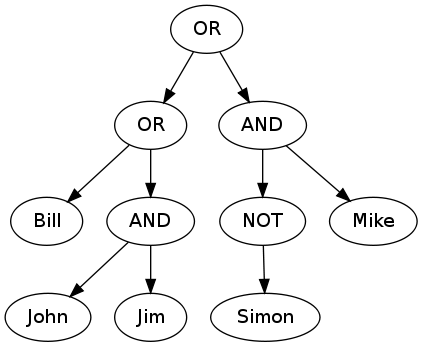
\includegraphics[width=2in]{midterm/syntax-tree.png}
\end{center}
\begin{enumerate}[(A)]
\item Write this tree as a Boolean expression using 
Boolean connectives ($\neg$, $\wedge$, etc.).
\item Write the same expression and ensure that it does not 
use any unnecessary parentheses (precedence and associativity is 
same as in Question 2). 
\item Write an equivalent expression using just two Boolean 
connectives (negation $\neg$ and disjunction $\vee$). 
\end{enumerate}


\subsubsection{A2. Sets and Quantifiers}

{\bf Question 4.} 
The universe $U$ is all integers between $1$ and $600$. 
$K_2 \subseteq U$ denotes all even numbers from $U$.
Similarly, $K_3 \subseteq U$ denotes all numbers divisible by $3$; 
$K_5 \subseteq U$ denotes all numbers divisible by $5$. 

\begin{enumerate}[(A)]
\item Draw Euler-Venn diagram with a big rectangle (the set $U$), 
the subsets $K_2$, $K_3$, $K_5$ as three intersecting circles.
\item Shade the region that corresponds to the set
$(K_2 \cap \overline K_3) \cup K_5$. 
\item Find the cardinality of the set
$\left| (K_2 \cap \overline K_3) \cup K_5 \right|$, 
justify your answer. 
\item Describe, which elements are in the set 
$(K_2 \cap \overline K_3) \cup K_5$ in English. 
For example: {\em ``All ... such that ... is divisible ... 
and/or is not divisible...''}. 
\end{enumerate}

\vspace{6pt}
{\bf Question 5.} 
In these pictures a red square on the intersection 
of row $i$ and column $j$ 
means that the predicate $L(i,j)$ is true (person $i$ 
loves person $j$). White square means that the predicate $L(i,j)$
is false. Here 
$i,j \in \{ \mathtt{a},\mathtt{b},\mathtt{c},\mathtt{d},\mathtt{e} \}$. 
\begin{center}
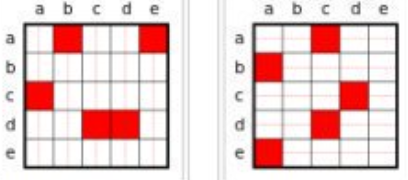
\includegraphics[width=2in]{midterm/predicate-grid.png}
\end{center}
Which statement is shown in the left picture?
\begin{enumerate}[(A)]
\item Everyone is loved by someone.
\item Eveyone loves someone.
\item Someone loves everyone.
\item Someone is loved by everyone.
\end{enumerate}
Which statement is shown in the right picture?
\begin{enumerate}[(A)]
\item $\forall x\, \exists y,\;L(y,x)$. 
\item $\forall x\, \exists y,\;L(x,y)$. 
\item $\exists x\, \forall y,\;L(x,y)$. 
\item $\exists x\, \forall y,\;L(y,x)$. 
\end{enumerate}




\subsubsection{A3. Algorithms and Big-O Notation}

In these problems you can verify the definition of the Big-O Notation 
or find the limit $f(n)/g(n)$ as $n \rightarrow \infty$. 

{\bf Question 6.} For each function find the smallest
$k$ such that $f(n)$ is in $O(n^k)$. Justify your answer.
\begin{enumerate}[(A)]
\item $f(n) = \sum_{j=1}^{n} (j^3 + j \log_2 j)$. 
\item $f(n) = n^3 + \sin n^7$. 
\item $f(n) = 1^2 + 2^2 + \ldots + n^2$.
\end{enumerate}

\vspace{6pt}
{\bf Question 7.} We say that the functions $f(n)$ and $g(n)$
{\em are of the same order}, if $f(n)$ is in $O(g(n))$ and
$g(n)$ is in $O(f(n))$. Find all pairs of functions in this 
list that are of the same order:
$$n^2 + \log_2 n,\; 2^n + 3^n,\; 100n^3 + n^2,\; n^2 + 2^n,$$
$$n^2 + n^3,\;3n^3 + 2^n.$$






\subsubsection{A4. Number Theory}


{\bf Question 8.}
\begin{enumerate}[(A)]
\item
Somebody has written a long hexadecimal number
{\tt F0F0F0...F0F} \textendash{} it uses $28$ digits "F"
separated by $27$ digits "0". 
Express the value of this number as a short expression
(without $\ldots$), using
the formula of a geometric progression: $\frac{b_1(q^{n+1}-1)}{q - 1}$. 
\item 
Somebody has written an infinite hexadecimal fraction 
{\tt 0.F0F0F0\ldots}. Express it as a rational number in 
decimal notation. 
\end{enumerate}



\vspace{6pt}
{\bf Question 9.} 
\begin{center}
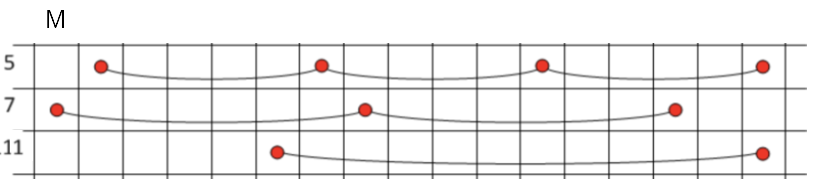
\includegraphics[width=3in]{midterm/sequences.png}
\end{center}

\begin{enumerate}[(A)]
\item Find some number $M \in \mathbb{Z}^{+}$ 
that gives the following remainders when divided by 
$5$, $7$ and $11$: 
$$\left\{
\begin{array}{l}
M \equiv 4\;(\text{mod}\,5)\\
M \equiv 0\;(\text{mod}\,7)\\
M \equiv 6\;(\text{mod}\,11)
\end{array} \right.$$
\item Find the arithmetic progression containing all such numbers $M$.
\end{enumerate}



\vspace{6pt}
{\bf Question 10.} 
\begin{enumerate}[(A)]
\item Alice has $13$-cent coins; Bob has $21$-cent coins. 
Alice wants to pay Bob exactly $1$ cent. How to do this?
\item Alice has $21$-cent coins; Bob has $13$-cent coins. 
Alice wants to pay Bob exactly $1$ cent. How to do this?
\item Solve the congruence equation \textendash{} find
$x$ such that $13x \equiv 1\;(mod\;21)$. 
\item Solve the congruence equation \textendash{} find
$x$ such that $13x \equiv 4\;(mod\;21)$. 
\end{enumerate}


\vspace{6pt}
{\bf Question 11.} 
\begin{enumerate}[(A)]
\item Write all positive powers of number $2$ ($2^1, 2^2, 2^3,\ldots$) modulo $11$ until 
you find a loop: i.e. some remainder repeats itself. How long is the period?
\item Write all negative powers of number $2$ modulo $13$ ($2^{-1},2^{-2},2^{-3},\ldots$) until 
you find a loop. How long is the period?
\end{enumerate}

{\em Note.} A negative power, for example $2^{-k}$ is such that $2^{-k}\cdot 2^k \equiv 1\;(\text{mod}\;11)$. 





\subsection{Part B. Analysis Tasks}

In these problems you have to apply concepts 
(such as predicates or quantifiers) to new situations, 
describe algorithms or procedures for new tasks
or sort cases in adaptive ways.


\subsubsection{B1. Propositional Logic}

{\bf Question 12.}
Among the people $A,B,C$ one is a truth-teller, 
the other two are liars. 
Every person ($A$, $B$, and $C$) has a closed box
in front of himself/herself. Exactly one of the 
boxes has a candy inside. $A,B,C$ know everything 
about each other and the location of candy.\\
Find out, which YES/NO questions you 
need to ask to find out, which box contains candy. 
Ask as few questions as possible 
(``brute-force'' strategies that ask clearly redundant
questions may only get partial credit). 

\vspace{6pt}
{\bf Question 13.} 
\begin{enumerate}[(a)]
\item Find out, if this formula is a tautology: 
$$\mathtt{((A \vee B) \wedge (A \rightarrow C) \wedge 
(B \rightarrow C)) \rightarrow C}.$$
\item Find out, if this formula is satisfiable: 
$$\mathtt{\neg (((A \vee B) \wedge (A \rightarrow C) \wedge 
(B \rightarrow C)) \rightarrow C)}.$$
\end{enumerate}

{\em Note.} A Boolean expression is called {\em tautology}, 
if it is true for all 
possible truth values of its variables. 
An expression is called {\em satisfiable}, 
if there is a way to assign 
variables so that it becomes true. 

\vspace{6pt}
{\bf Question 14.} 
Let us have three people \textendash{} Ada, Barbara and Cecilia. 
Every day some of them are charging batteries for Lego robots.
Let us have propositional variables $a,b,c$ (a variable $a,b,c$ is true, iff 
today batteries were charged by Ada, Barbara or Cecilia respectively). 

Write a Boolean expression telling that today batteries were charged
by {\bf exactly} two people out of the three. You can use variables $a,b,c$ and
all $5$ Boolean connectives ($\neg$, $\vee$, $\wedge$, $\rightarrow$, 
$\leftrightarrow$). 



\subsubsection{B2. Sets and Quantifiers}

{\bf Question 15.} We define the set of all bounded functions defined on the interval $(a;b)$ 
as functions that have all their values between two bounds: there is a positive number $M$
such that all all values of the function $f$ are in the interval $[-M;M]$. With predicates and quantifiers:
$$\exists M \in \mathbb{R}^{+},\,\forall x \in \mathbb{R}\,\;x \in (a;b) \rightarrow |f(x)| \leq M.$$
In this picture one of the functions (the red one) is bounded, the other one is unbounded.
\begin{center}
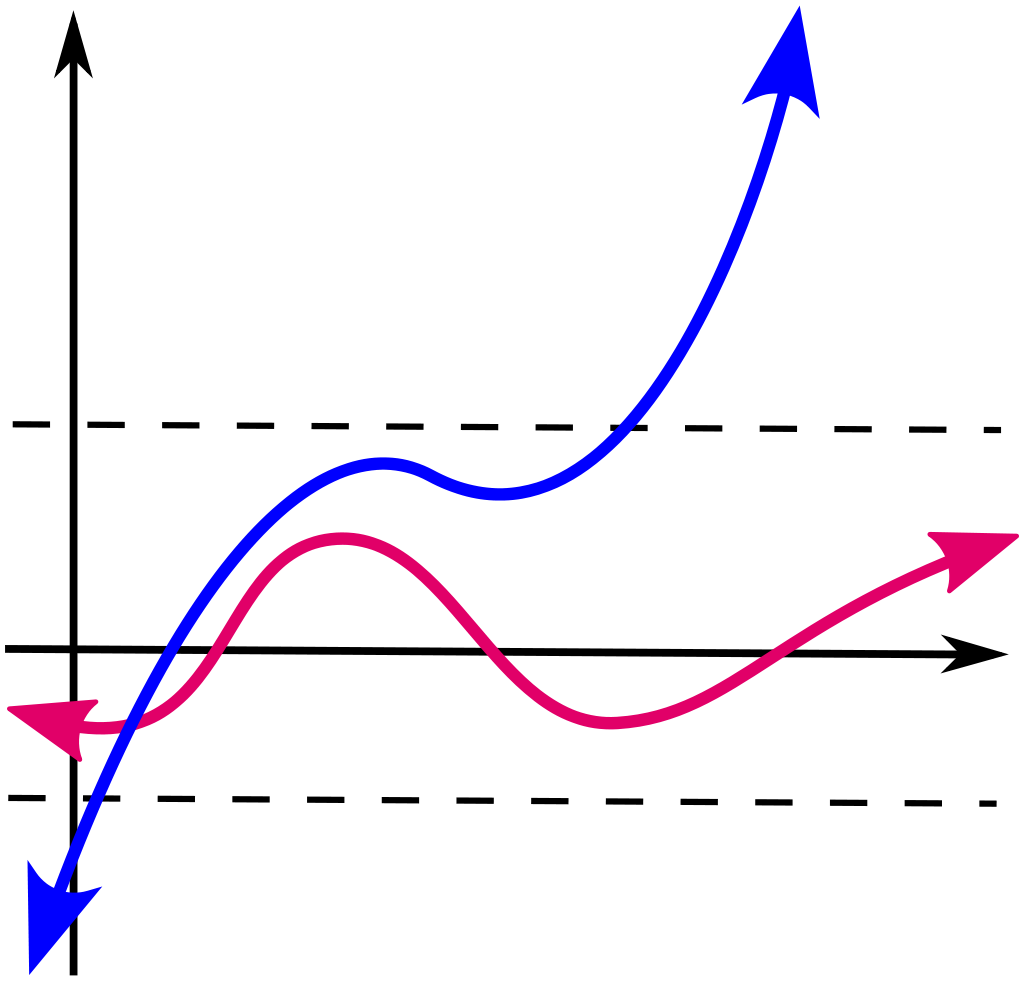
\includegraphics[width=2in]{midterm/bounded-function.png}
\end{center}
\begin{enumerate}[(A)]
\item Write an expression with predicates and quantifiers to express the statement: 
``Function $f:(a;b) \rightarrow \mathbb{R}$ is {\bf not} bounded.''
\item Find an example of a function that is defined and bounded in the interval $(0;1)$. 
\item Find an example of a function that is defined, but unbounded in the interval $(0;1)$. 
\item What functions are described by another predicate logic expression, where we switch the order of quantifiers:
$$\forall x \in \mathbb{R}\,\exists M \in \mathbb{R}^{+},\;x \in (a;b) \rightarrow |f(x)| \leq M.$$
\end{enumerate}


\vspace{6pt}
{\bf Question 16.} An infinite sequence $a_0,a_1,a_2,\ldots$ is called {\em purely periodic}, if 
all the members of it repeat the same finite pattern over and over again. 
For example, $3,3,3,3,\ldots$ or $1,3,1,3,1,3,\ldots$ are purely periodic. 
Meanwhile, 
$1,6,6,6,6,\ldots$ or $1,4,1,4,2,1,3,5,\ldots$ (the digits of $\sqrt{2}$) 
are not purely periodic (they are either ``eventually periodic'' with some digits preceding the period 
or not periodic at all). 
\begin{enumerate}[(A)]
\item Write an expression to tell that a given sequence $(a_n)_{n \in \mathbb{N}}$ 
is purely periodic. 
\item Write an expression to tell that a given sequence $(a_n)_{n \in \mathbb{N}}$ 
is {\bf NOT} purely periodic. 
\end{enumerate}


\vspace{6pt}
{\bf Question 17.} 
Consider the set $A = \{ 1,2,3,4,6,12 \}$. We define a
predicate 
$$P \,:\, A \times A \rightarrow \{ \mathtt{True}, \mathtt{False} \},$$
where $P(i,j)$ is true iff the divisibility by $i$ implies 
divisibility by $j$ (for any $i,j \in A$). 
For example $P(12,2) = \mathtt{True}$, since any number 
that is divisible by $i = 12$ is also divisible by $j=2$. 

\begin{enumerate}[(A)]
\item Is the 2-argument predicate $P$ {\em reflexive} \textendash{}
does it satisfy the logic formula:
$$\forall i \in A,\;P(i,i).$$
\item Is the predicate $P$ {\em symmetric} \textendash{}
does it satisfy the logic formula:
$$\forall i \in A,\,\forall j \in A,\;P(i,j) \rightarrow P(j,i).$$
\item Is the predicate $P$ {\em transitive} \textendash{}
does it satisfy the logic formula:
$$\forall i,j,k \in A,\;P(i,j) \wedge P(j,k) \rightarrow P(i,k).$$
\item Is the predicate $P$ {\em connex} \textendash{}
does it satisfy the logic formula:
$$\forall i,j \in A,\;P(i,j) \vee P(j,i).$$
\end{enumerate}

{\em Note 1.} Even though the predicate formulas can be verified
by checking all possible combinations of $i,j,k \in A$ (the set $A$ is finite), 
it is much faster to reason by the properties of divisibility.\\
{\em Note 2.} For each statement either add a short justification or provide
a counterexample.






\subsubsection{B3. Algorithms and Big-O Notation} 

{\bf Question 18.} Let $A,B$ be subsets from the same universe $U = \{ 1,2,\ldots,n \}$. 
We want to find the intersection of these two sets $A \cap B$. 

\begin{enumerate}[(A)]
\item Describe an algorithm (using steps written in English or some pseudocode) 
to find and to output all numbers that are in this intersection $A \cap B$. 
(You can call the algorithms that are in the K.Rosen's textbook - for sorting, 
linear or binary search and similar. But write out your assumptions, so that it is unambiguous, 
which method you are using.)
\item Estimate the time complexity $O(f(n))$: provide a function that estimates the 
worst-case time required as the size of the universe $U$ grows.
\end{enumerate}

\vspace{6pt}
{\bf Question 19.} 
\begin{enumerate}
\item 
Prove that $f(n) = n^2 + n \cdot \ln n$ is in $O(n^2)$ (i.e. $g(n) = n^2$) by finding the limit
of the ratio:
$$\lim_{n \rightarrow \infty} \frac{n^2 + n \cdot \ln n}{n^2}.$$
Or by directly checking the definition of the Big-O notation (finding the two 
constants $C$ and $k$ that give you the estimate: 
$n>k \rightarrow |f(n)| \leq C|g(n)|$.
\item Is the function $g(n) = n^2$ also in $O(f(n))$, where $f(n) = n^2 + n \cdot \ln n$? 
Once again, justify by finding a limit or by checking the definition.
\end{enumerate}





\subsubsection{B4. Number Theory} 


{\bf Question 20.} Let us consider the following statement:\\

{\bf Bezout's identity:} 
Let $a$ and $b$ be integers and $d$ is their greatest common divisor: $\text{gcd}(a,b)=d$. 
Then, there exist integers $x$ and $y$ such that $ax + by = d$.\\

\begin{enumerate}[(A)] 
\item Let us have parameters $a,b \in \mathbb{Z}$ and $d \in \mathbb{Z}^{+}$ such that $\text{gcd}(a,b)=d$. 
Write the Bezout's identity using predicates and quantifiers (you can also 
use equality and four arithmetic operations). 
\item Using the same notation as before, write another statement using predicates and quantifiers: 
``The modular equation $ax\equiv{}c\;(\text{mod}\,b)$ has a solution if and only if 
$c$ is a multiple of $d$.''
\item Using the same notation as before, write another statement using predicates and quantifiers: 
``The greatest common divisor $d$ is the smallest positive integer that can be expressed as $ax+by$ for 
the given $a,b$ and any integers $x,y$.''
\end{enumerate}

{\em Note 1.} In this expression $a,b,c,d$ are {\em free variables}; they are given and can be used in your formulas. 
You can also use any number of {\em bound variables}.\\
{\em Note 2.} We call $c$ a {\em multiple} of $d$ iff $c$ can be expressed as some integer number times $d$.

\vspace{6pt}
{\bf Question 21.} Somebody has proposed a way to encode finite sequences of natural numbers $\mathbb{N}$
(i.e. nonnegative integers: $\mathbb{N} = 0,1,2,\ldots$) as natural numbers. 
To encode a sequence $(a_1,a_2,\ldots,a_k)$ we take the first $k$ primes
($p_1 = 2$, $p_2 = 3$, $p_3 = 5$, and so on) and build a number: 
$$f(a_1,a_2,\ldots,a_k) = p_1^{a_1}p_2^{a_2}p_3^{a_3}\ldots$$
For example, the sequence $(1,0,2)$ is encoded as $2^1\cdot{} 3^0 \cdot 5^2 = 50$, 
but the sequence $(1,1,1,1)$ is encoded as $2^1 \cdot 3^1 \cdot 5^1 \cdot 7^1 =  210$.
\begin{enumerate}
\item Is the function $f: \mathbb{N}^{\ast} \rightarrow \mathbb{N}$ a surjection?
\item Is the function $f: \mathbb{N}^{\ast} \rightarrow \mathbb{N}$ an injection?
\item Can you suggest a bijective function $g: \mathbb{N}^{\ast} \rightarrow \mathbb{N}$ to encode any finite sequence of natural numbers 
with a single natural number?
\end{enumerate}

{\em Note.} By $\mathbb{N}^{\ast}$ we denote a list of all finite tuples: 
$$\mathbb{N}^{\ast} = \{()\} \cup (\mathbb{N}) \cup (\mathbb{N} \times \mathbb{N}) \cup \ldots.$$
It contains one list of length $0$,\\
It contains $(\mathbb{N})$ all single-element lists $(0)$, $(1)$, etc.,\\
It contains $(\mathbb{N} \times \mathbb{N})$, i.e. all two-element pairs $(0,0)$, $(0,1)$, $(1,0)$, $(1,1)$, etc.\\
And so on.

\vspace{6pt}
{\bf Question 22.} Consider the set of all square functions ($f:\mathbb{R} \rightarrow \mathbb{R}$)
that can be expressed as $f(x) = ax^2 + bx + c$ with integer coefficients $a,b,c$. 
Is the set of all such square functions finite? countable? uncountable? 
Justify your answer.





\subsection{Part C. Proofs}

In proof problems the goal is to prove some general statement by 
showing every essential step of your reasoning.
Below we describe various proof strategies and give some sample
statements that can be proven by that strategy.

\vspace{6pt}
{\bf Translate into Algebra}

In K.Rosen's textbook these are called ``direct proofs''
of IF-THEN statements. 
You assume that the condition is true, introduce some notation and 
prove that also the conclusion is true.
You sometimes need to sort cases. 

\vspace{6pt}
{\bf Question 23.} Prove that, if $n$ is odd, then $n^2$ is also odd. 

\vspace{6pt}
{\bf Question 24.} Prove that, if the decimal notation of a number $n$ ends with the digit "5", 
then $n^2$ ends with digits "25". 

\vspace{6pt}
{\bf Question 25.}
Prove that $n^2 \equiv 5\;(\text{mod}\;11)$ is true
iff
$n \equiv 4\;(\text{mod}\;11)$ 
or $n \equiv -4\;(\text{mod}\;11)$.

\vspace{20pt}
{\bf Proofs by Contradiction}

In these examples you assume that the statement is false
and get a contradiction.


\vspace{6pt}
{\bf Question 26.} Prove that there are infinitely many primes.

\vspace{6pt}
{\bf Question 27.} Prove that there are infinitely many primes of the form $4n+3$. 

\vspace{6pt}
{\bf Question 28.} Prove that there are infinitely many primes
that divide some value of the polynomial 
$P(n) = n^2 + n + 1$. 

\vspace{6pt}
{\bf Question 29.}
Prove that $\sqrt{2}$ is irrational.

\vspace{6pt}
{\bf Question 30.}
$\log_2 10$ is irrational.


\vspace{20pt}
{\bf Building Bijective Functions (Countable)}

Any combinations of these tactics can be used
to prove that two sets have the same cardinality
(and that there is a bijective function from one set to another).

\vspace{6pt}
{\bf Question 31.}
There is a bijection from $\mathbb{Z}^{+} \cup \{ 1,2,\ldots,n \}$
to $\mathbb{Z}^{+}$.\\
{\em Hint.} One can add $n$ new guests to the Hilbert's hotel.

\vspace{6pt}
{\bf Question 32.}
There is a bijection from $\mathbb{Z}^{+} \times \{ 1,2 \}$
to $\mathbb{Z}^{+}$.\\
{\em Hint.} If there are two infinite buses with guests: 
$(1,1),(2,1),(3,1),\ldots$ and $(1,2),(2,2),(2,3),\ldots$, 
then they can be hosted in a single Hilbert's hotel.

\vspace{6pt}
{\bf Question 33.}
There is a bijection from $\mathbb{Z}^{+} \times \mathbb{Z}^{+}$
to $\mathbb{Z}^{+}$.\\
{\em Hint.} Show how infinitely many infinite buses can be hosted in a 
single Hilbert's hotel (similar to Question 9 from HW1).

\vspace{6pt}
{\bf Question 34.}
There is a bijection from $\mathbb{Q}$ to $\mathbb{Z}^{+}$.\\
{\em Hint.} Same as above, but now you need to combine
three sets of numbers into the same Hilberts hotel (positive rationals, 
negative rationals and $0$). 

\vspace{20pt}
{\bf Building Bijective Functions (Uncountable)}

\vspace{6pt}
{\bf Question 35.}
There is a bijective function from any closed 
segment $[a;b]$ to any other closed segment $[c;d]$
(regardless of their lengths).\\
{\em Hint.} This can be achieved by a simple linear function.

\vspace{6pt}
{\bf Question 36.}
There is a bijective function from any open 
segment $(a;b)$ to any other open segment $(c;d)$.\\
{\em Hint.} This also can be achieved by a linear function. 

\vspace{6pt}
{\bf Question 37.}
There is a bijective function from any open 
segment $(a;b)$ to the set of all real numbers $\mathbb{R}$
or to the half-line of all positive reals $(0;+\infty)$.\\
{\em Hint.} You can use a continuous function with one or two 
vertical asymptotes. Such as $f(x) = x/(1-x)$ or $f(x) = \tan x$.

\vspace{6pt}
{\bf Question 38.}
There is a bijective function from a 
semi-open segment $[0;1)$ to an open segment $(0;1)$.\\
{\em Hint.} Map the extra point (argument $x = 0$) to any 
point inside the target interval $(0;1)$, then 
change values for an infinite sequence (bounded inside $(0;1)$)
in the same way as Hibert's hotel. 


\vspace{20pt}
{\bf Proving there is no Bijection}

All these proofs use Cantor's diagonalization. (See subsection 
``2.5.3 An uncountable set'' in the textbook; pp. 183-187.)

\vspace{6pt}
{\bf Question 39.} Numbers on $(0;1)$ are uncountable.


\vspace{6pt}
{\bf Question 40.}
 All real numbers $\mathbb{R}$ are uncountable - there 
is no bijection from $\mathbb{R}$ to $\mathbb{Z}^{+}$ or
to $\mathbb{Q}$. 


\vspace{6pt}
{\bf Question 41.} All infinite sequences of integers are uncountable
(Also, all non-decreasing sequences of integers are uncountable.


\vspace{6pt}
{\bf Question 42.} The Power-set of any countable set is 
uncountable. For example, 
there is no bijection from $\mathcal{P}(\mathbb{Z}^{+})$
to $\mathbb{Z}^{+}$ (i.e. no mapping from the set of all subsets of 
positive integers to the set of integers themselves).





\end{document}



\newpage
\documentclass[jou]{apa6}

\usepackage[american]{babel}

\usepackage{csquotes}
\usepackage[style=apa,sortcites=true,sorting=nyt,backend=biber]{biblatex}
\DeclareLanguageMapping{american}{american-apa}
\addbibresource{bibliography.bib}


%%%%%%%%%%%%%%%%%%%%%%%%%%%%%%%%%%%%%%%%
%% Discrete Structures
%% The start of RBS stuff
%%%%%%%%%%%%%%%%%%%%%%%%%%%%%%%%%%%%%%%%

% Working internal and external links in PDF
\usepackage{hyperref}
% Extra math symbols in LaTeX
\usepackage{amsmath}
\usepackage{gensymb}
\usepackage{amssymb}
% Enumerations with (a), (b), etc.
\usepackage{enumerate}

\let\OLDitemize\itemize
\renewcommand\itemize{\OLDitemize\addtolength{\itemsep}{-6pt}}

\usepackage{etoolbox}
\makeatletter
\preto{\@verbatim}{\topsep=3pt \partopsep=3pt }
\makeatother

% These sizes redefine APA for A4 paper size
\oddsidemargin 0.0in
\evensidemargin 0.0in
\textwidth 6.27in
\headheight 1.0in
\topmargin -24pt
\headheight 12pt
\headsep 12pt
\textheight 9.19in



\setlength\parindent{0pt}

\title{Midterm, 2020-02-17}
\author{Discrete Structures, Fall 2020}
\affiliation{RBS}

\leftheader{Midterm, 2020-02-17}

\abstract{%
}

%\keywords{}

\begin{document}

%\thispagestyle{empty}

\twocolumn
\section{Midterm, 2020-02-17}

\vspace{6pt}
{\bf Question 1 (Boolean Expressions).}\\
Consider Boolean expression:
$$E_0 = (p \rightarrow q \rightarrow r) \wedge (q \rightarrow r \rightarrow p) \wedge (r \rightarrow p \rightarrow q)$$
\begin{center}
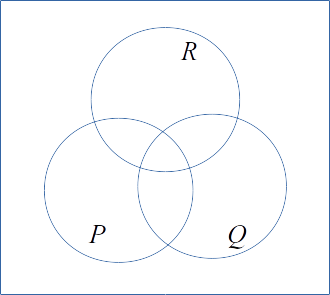
\includegraphics[width=2in]{midterm/circles.png}
\end{center}

\begin{enumerate}[(A)]
\item Copy the Venn diagram's circles in your solution and shade those regions in the diagram that make $E_0$ true
(being inside each circle $P,Q,R$ means that the respective variable $p,q,r$ is true; being outside the circle means
that the variable is false). 
\item In the truth table of $E_0$ how many entries are $\mathtt{True}$?\\
({\em Note.} Building the truth table is optional. Regardless whether you build one or not, you should justify your answer.)
\item Rewrite the Boolean expression $E_0$ into an equivalent one, using 
only conjunctions ($\wedge$) and negations ($\neg$). 
\end{enumerate}

Assume that implication ($\rightarrow$) is right-associative 
and conjunction ($\wedge$) has higher precedence than implication. 



\vspace{10pt}
{\bf Question 2 (Nested Quantifiers).}\\
Verify, if the following predicate/quantifier expressions are true for the given predicate. 
The predicate $P$ is defined on $A \times A$, where
$A = \{ \mathtt{a},\mathtt{b},\mathtt{c},\mathtt{d},\mathtt{e},\mathtt{f} \}$. 
Predicate $P(\mathtt{a},\mathtt{b})$ is true iff the square on row $\mathtt{a}$
and column $\mathtt{b}$ is shaded (and the predicate $P(\mathtt{a},\mathtt{b})$ 
is false, if that square is white).

\begin{center}
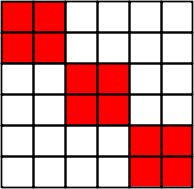
\includegraphics[width=1.2in]{midterm/relation.png}
\end{center}

\begin{enumerate}[(A)]
\item Does the predicate $P$ satisfy the logic formula:
$$\forall i \in A,\;P(i,i).$$
\item Does the predicate $P$ satisfy the logic formula:
$$\forall i \in A,\,\forall j \in A,\;P(i,j) \rightarrow P(j,i).$$
\item Does the predicate $P$ satisfy the logic formula:
$$\forall i,j,k \in A,\;P(i,j) \wedge P(j,k) \rightarrow P(i,k).$$
\item Does the predicate $P$ satisfy the logic formula:
$$\forall i,j \in A,\;P(i,j) \vee P(j,i).$$
\item Does the predicate $P$ satisfy the logic formula:
$$\forall i \in A,\, \exists j \in A,\;P(i,j).$$
\end{enumerate}

\vspace{10pt}
{\bf Question 3 (Estimate with Big-O Notation).}\\
Define the sequence $S(n)$ as a sum of squares from $1^2$ to $n^2$:
$$S(n) = \sum\limits_{i=1}^n i^2.$$
We have $S(1) = 1^2 = 1$, $S(2) = 1^2 + 2^2 = 5$, 
$S(3) = 1^2 + 2^2 + 3^2 = 14$,
and so on. 

\begin{enumerate}[(A)]
\item Is the function $S(n)$ in $O(n^1)$? 
Is it in $O(n^2)$? Is it in $O(n^3)$? Is it in $O(n^4)$? 
Explain your reasoning. 
\item Pick any one of the notations from the previous items 
($g(n)$ is either $O(n^1)$, or $O(n^2)$, or $O(n^3)$, or $O(n^4)$). 
Check the definition of Big-O notation: Find the {\em witness}: the value $k$ and the constant $C$
such that the absolute value of $S(n)$ does not exceed $C\cdot{}|g(n)|$ for all $n > k$.
\end{enumerate}


\vspace{10pt}
{\bf Question 4 (Chinese Remainder Theorem).}

Consider the following system of three congruences:
$$\left\{ \begin{array}{l}
x \equiv 1\;(\text{mod}\,5),\\
x \equiv 2\;(\text{mod}\,7),\\
x \equiv 3\;(\text{mod}\,9).
\end{array} \right.$$

\begin{enumerate}[(A)]
\item Does it have a solution? Will it have solution, even if we replace $1,2,3$ with other numbers
on the right sides of the equation.
\item Find an arithmetic progression (what is its first member $A$, difference $B$) where all members satisfy
the first two congruences from the system.
\item Find an arithmetic progression (what is its first member $C$, difference $D$) where all members satisfy
all three congruences in the system.
\end{enumerate}

{\em Note.} Arithmetic progression is an infinite sequence where every next member can be obtained
by adding the same number (the difference) to the previous one. For example, 
$$A,\;A+B,\;A+2B,\;A+3B,\ldots$$
is an arithmetic progression with the first member $A$ and the difference $B$.


\vspace{10pt}
{\bf Question 5 (Binary notation).}

Somebody has written two binary fractions on the board: $\alpha$ is infinite, $\beta$ is finite (just $6$ digits
after the point): 
$$\left\{ \begin{array}{l}
\alpha = 0.(011110)_2 = 0.011110011110011110\ldots_2\\
\beta = 0.011110_2.
\end{array} \right.$$

\begin{enumerate}[(A)]
\item Express the number $\beta$ as a sum of some negative powers of $2$; 
namely, show how to add up some of the numbers
$$\{ 2^{-1}, 2^{-2}, 2^{-3}, \ldots \}$$ 
to get $\beta$. 
\item Express $\beta$ as an irreducible fraction {\tt P/Q}; write this in the regular decimal notation. 
\item Write the product $64_{10} \cdot \alpha = 1000000_2 \cdot \alpha$ in the binary notation. 
\item Express $\alpha$ as an irreducible fraction {\tt P/Q} in decimal notation.
\end{enumerate}



\vspace{10pt}
{\bf Question 6 (Truth-tellers and Liars).}
Among the people $A,B,C$ one is a truth-teller, 
the other two are liars. 
Every person ($A$, $B$, and $C$) has a closed box
in front of himself/herself. Exactly one of the 
boxes has a candy inside. $A,B,C$ know everything 
about each other and the location of candy.

Someone else (person $D$) approaches all of them. $D$ knows, who are 
people $A$,$B$, and $C$ (it is written on their name-cards), but $D$ does
not know anything about their lying behavior or the location of the candy.
$D$ is allowed to ask YES/NO questions to one or more people.

\begin{enumerate}[(A)]
\item Can $D$ find out who has the candy by asking three questions?
\item Can $D$ find out who has the candy by asking two questions?
\item Can $D$ find out who has the candy by asking one question?
\end{enumerate}

Justify your answers (by construction or by showing that it is impossible).


\vspace{10pt}
{\bf Question 7 (Time Complexity of Truth Tables).}

Assume that there is a Boolean expression $E$ with $n$ variables: 
$$E = E(a_1,a_2,\ldots,a_n).$$
The expression $E$ contains $2n$ Boolean operators (such as $\neg$, $\wedge$, $\vee$).
Variables $a_1,a_2,\ldots,a_n$ can independently take values 
$\mathtt{True}$ or $\mathtt{False}$.

Consider the following algorithm to find, if $E$ is a tautology by 
building the truth table. We will either find a false value, or 
establish that all values were true (in this case $E$ is a tautology).

{\bf (1)} \hspace{0.0in} For each assignment of $n$ truth values to $a_1,\ldots,a_n$:\\
{\bf (2)} \hspace{0.2in} For each of the $2n$ Boolean operators in $E$:\\
{\bf (3)} \hspace{0.4in} Compute the value of that Boolean operator\\
{\bf (4)} \hspace{0.2in} If $E$ has value $\mathtt{False}$:\\
{\bf (5)} \hspace{0.4in} Return ``$E$ is not a tautology.''\\
{\bf (6)} \hspace{0.2in} If $E$ has value $\mathtt{True}$:\\
{\bf (7)} \hspace{0.4in} Continue loop on Line {\bf (1)}.\\
{\bf (8)} \hspace{0.0in} Return ``$E$ is a tautology.''

\begin{enumerate}[(A)]
\item Find the worst-case runtime $T(n)$ for this algorithm as an expression of $n$.
(Assume that evaluating one Boolean operator $\neg$, $\wedge$, $\vee$ takes $1$ unit of time.)
\item Find a function $g(n)$ such that $T(n)$ is in $O(g(n))$. 
\end{enumerate}




\vspace{10pt}
{\bf Question 8 (About Rational and Irrational).}

We denote two real numbers by $p$ and $q$. 
Prove or disprove statements about the rational and irrational numbers. 

\begin{enumerate}[(A)]
\item If $p + q$ is rational, then either both $p,q$ are rational, or both are irrational. 
\item If $pq$ is rational, then either both $p,q$ are rational, or both are irrational. 
\item If $p^2$ and $q^2$ are both rational, then the product $(p+q)(p-q)$ is rational. 
\item If $p^3$ and $p^5$ are both rational, then $p$ is rational.
\item If $pq$ and $p+q$ are both rational, then $p$ and $q$ are both rational.
\end{enumerate}

\newpage

\subsection{Answers}

{\em Note. Grading criteria (see the tables below) should not be considered as a dogma, 
since every work is different. They provide some guidelines how the points typically split. 
There are 10 points (maximum) for any given problem. If the problem has multiple parts
({\bf (A)}, {\bf (B)}, etc.) each part is allocated certain portion of these points. 
There are 1-2 points that can be added or subtracted depending on how clearly the 
partial solution is written.}

{\em
The theoretical maximum for the whole midterm is 80 points (all 8 problems solved for 10 points each).
Since the midterm accounts for 150~\textperthousand{} (150 promilles or 15 percent) of your
total grade; we get the total grade (in promilles) by multiplying your points by 2
(and cutting it to the maximum value 150~\textperthousand{}, if necessary). 
}

\vspace{6pt}
{\bf Question 1}\\
{\bf (A)} The only way to have $p \rightarrow q \rightarrow r = p \rightarrow (q \rightarrow r)$ evaluate to 
$\mathtt{False}$ is $p = \mathtt{True}$ and $(q \rightarrow r) = \mathtt{False}$ (i.e.\ 
$q = \mathtt{True}$ and $r = \mathtt{False}$).\\
If we consider also $q \rightarrow r \rightarrow p$ and $r \rightarrow p \rightarrow q$, there are two 
more ways to get the whole expression $E_0$ false. Each of these ways means that exactly two variables
are $\mathtt{True}$ and the third one is $\mathtt{False}$. 
All the other areas make the expression true. Shaded areas look like shown below. There are just $3$ 
regions where the expression $E_0$ evaluates to false (white, not shaded). 
\begin{center}
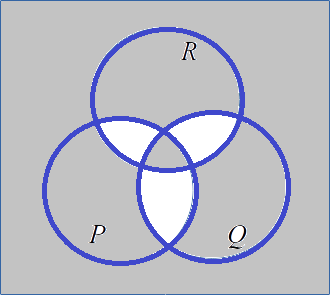
\includegraphics[width=2in]{midterm/circles-shaded2.png}
\end{center}

{\bf (B)} There are exactly $8-3 = 5$ entries in the truth table which make the expression true
(there are only $3$ ways to make the expression false, as shown in {\bf (A)}). 

{\bf (C)} Let us just transform one subexpression: 
\begin{align}
 & p \rightarrow (q \rightarrow r) = \nonumber \\
= & \neg p \vee (q \rightarrow r) = \nonumber \\
= & \neg p \vee (\neg q \vee r) = \nonumber \\
= & \neg p \vee \neg q \vee r  = \nonumber \\
= & \neg (p \wedge q \wedge \neg r). \nonumber
\end{align}

If we combine all $3$ subexpressions (where $p,q,r$ switch their order), we get 
a longer conjuction for $E_0$:

$$\neg (p \wedge q \wedge \neg r) \wedge \neg (q \wedge r \wedge \neg p) \wedge \neg (r \wedge p \wedge \neg q).$$

{\footnotesize
\begin{tabular}{|l|l|} \hline
{\bf (A)} Shading is correct & 3 points \\ \hline
{\bf (A)} Shading incorrect, but matches truth table & 2 points \\ \hline
{\bf (B)} Truth table or explanation for the number of ``true'' & 3 points \\ \hline
{\bf (B)} Partial truth table or incomplete justification & 2 points \\ \hline
{\bf (C)} Correct formula with conjunctions, negations & 4 points \\ \hline
\end{tabular}
}




\vspace{10pt}
{\bf Question 2}
\begin{enumerate}[(A)]
\item Yes, $\forall i \in A,\;P(i,i)$ is true (we say that the 2-argument predicate 
is {\em reflexive}): all the squares $P(i,i)$ on the diagonal of the values are shaded. 
\item Yes, $\forall i \in A,\,\forall j \in A,\;P(i,j) \rightarrow P(j,i)$ is true (we say that the 2-argument predicate 
is {\em symmetric}): the squares in the table of $P(i,j)$ are symmetric against
the diagonal of the values: $P(i,j)$ is shaded iff $P(j,i)$ is shaded.
\item Yes, $\forall i,j,k \in A,\;P(i,j) \wedge P(j,k) \rightarrow P(i,k)$ is true 
(we say that the 2-argument predicate 
is {\em transitive}). Notice that $P(i,j)$ can be true iff $i=j$ or $(i,j)$ is 
one of the pairs of neighbors: $(\mathtt{a},\mathtt{b})$, or $(\mathtt{c},\mathtt{d})$, or $(\mathtt{e},\mathtt{f})$.
$P(j,k)$ is also true; so $j,k$ also belong to the same pair. Therefore $i$ and $k$ also belong to the same pair. 
\item No, $\forall i,j \in A,\;P(i,j) \vee P(j,i)$ is false. For example, neither $P(\mathtt{a},\mathtt{c})$
nor $P(\mathtt{c},\mathtt{a})$ are true.
\item Yes, $\forall i \in A,\, \exists j \in A,\;P(i,j)$ is true: On each row $i$ there is at least
one shaded square.
\end{enumerate}

{\footnotesize
\begin{tabular}{|l|l|} \hline
{\bf (A)-(E)} Correct answer plus valid explanation & 2 points (for each) \\ \hline
{\bf (A)-(E)} Correct truth value & 1 point (for each) \\ \hline
\end{tabular}
}

\vspace{10pt}
{\bf Question 3}
{\bf (A)} $S(n)$ is in $O(n^3)$ (and therefore it is also in $O(n^4)$). 
On the other hand, $S(n)$ is not in $O(n^2)$ or $O(n^1)$.\\
Let us show that $S(n)$ is not in $O(n^2)$. Assume from the contrary
that there are numbers $k$ and $C$ such that for each $n > k$:
$$|S(n)| = |1^2 + 2^2 + \ldots + n^2| \leq C \cdot |n^2|.$$
Since all numbers there are positive, we drop the absolute values. 
We pick any even number $n > k$ which also satisfies $n > 8C$. In this case:
\begin{align}
 & S(n) = 1^2 + 2^2 + \ldots + n^2 > \nonumber \\
> & \left( \frac{n}{2} + 1 \right)^2 + \left( \frac{n}{2} + 2 \right)^2 + \ldots + n^2 > \nonumber \\
> & \frac{n}{2} \cdot \left( \frac{n}{2} \right)^2 \geq \frac{n}{8} \cdot n^2 \geq C n^2. \nonumber 
\end{align}
{\em (In these inequalities, we first drop the first half of the sum; 
then replace each term with $(n/2)^2$ and we still can prove that the sum is more than $Cn^2$ 
for the given constant $C$.)}\\
Such $n$ can always be found (no matter what $k$ and $C$ are used). 
Therefore $S(n)$ can never satisfy $|S(n)| \leq C \cdot n^2$.\\
Since $n$ is even smaller than $n^2$, $S(n)$ is not in $O(n)$ either. 

{\bf (B)} Let us prove that $S(n)$ is in $O(n^3)$. 
Let us pick the {\em witness} to check the definition of the Big-O Notation: 
$k = 1$, $C = 1$. 
\begin{align}
     & 1^2 + 2^2 + \ldots + n^2 \leq \nonumber \\
\leq\;\; & n^2 + n^2 + \ldots + n^2=  n \cdot n^2 = 1 \cdot n^3. \nonumber
\end{align}

{\footnotesize
\begin{tabular}{|l|l|} \hline
{\bf (A)} Answer $O(n^3)$ with explanation & 6 points \\ \hline
{\bf (A)} Answer $O(n^3)$ without explanation & 3 points \\ \hline
{\bf (A)} Suboptimal, but correct answer $O(n^4)$ & 2 points \\ \hline
{\bf (B)} Correct witness to show inequality & 4 points \\ \hline
\end{tabular}
}

\vspace{10pt}
{\bf Question 4}
{\bf (A)} Yes, the system will always have solution (even if you replace the numbers $1,2,3$ by 
any other integers). Chinese Remainder theorem only needs that the modules 
($5,7,9$ in our case) are mutually prime.

{\bf (B)} The numbers satisfying $x \equiv 1\;(\text{mod}\,5)$ make this arithmetic progression: 
$$1,\,6,\,11,\,16,\,21,\,26,\,31,\,\ldots$$
Number $16$ in this progression is also congruent to $2$ (modulo $7$). The next number would be 
$16 + 35 = 51$ (because adding $5 \cdot 7 = 35$ does not change the remainders, when 
we divide by $5$ or by $7$.\\
We conclude that the following arithmetic progression satisfies the top two congruences
(remainder $1$ modulo $5$ and remainder $2$ modulo $7$):
$$16,\,51,\,86,\,121,\,156,\,191,\,\ldots$$
Answer: $A = 16$, $B = 35$. 

{\bf (C)} Observe that the first member of this arithmetic sequence ($A = 16$) gives the
remainder $7$ when divided by $9$. The difference ($B = 35$) is congruent to $8$ and also to $-1$ 
modulo $9$.\\
We conclude that by adding four differences, the result is
$$16 + 4 \cdot 35 \equiv 16 + 4 \cdot (-1) \equiv 12 \equiv 3\;(\text{mod}\,9).$$
The first number from the progression (item (B)) that is also congruent to $3$ modulo $9$ is $156$. 
We can add $5 \cdot 7 \cdot 9 = 315$ to this number, and all the remainders will stay the same:
$$156,\,471,\,786,\,1101,\,1416,\,1731,\,2046,\,\ldots$$
Answer: $C = 156$, $D = 315$.

{\footnotesize
\begin{tabular}{|l|l|} \hline
{\bf (A)} Reasoning that $5,7,9$ are pairwise mutual primes & 2 points \\ \hline
{\bf (B)} $16+35k$ & 4 points \\ \hline
{\bf (B)} $16$, but wrong difference & 2 points \\ \hline
{\bf (C)} $156+315k$ & 4 points \\ \hline
{\bf (C)} $156$, but wrong difference & 2 points \\ \hline
\end{tabular}
}

\vspace{10pt}
{\bf Question 5}
{\bf (A)} $\beta = 0.011110_2 = 2^{-2} + 2^{-3} + 2^{-4} + 2^{-5}$.\\
{\bf (B)} $\beta = \frac{8 + 4 + 2 + 1}{2^{5}} = \frac{15}{32}$.\\
{\bf (C)} $64\alpha = 1000000_2 \cdot \alpha =$\\
$= 011110.011110011110011110\ldots_2$ (to multiply 
by $2^6 = 64$ we shift the point six positions to the right).
{\bf (D)} Subtract $\alpha$ from $64\alpha$: We get $011110_2$ (because all the 
digits after the point are the same \textendash{} they cancel out). We get the equation:
$$64\alpha - \alpha = 63\alpha = 011110_2 = 30_{10}$$
Therefore $\alpha = \frac{30}{63} = \frac{10}{21}$. We could also get the
same answer by finding the sum of an infinite geometric progression: 
$$30 \cdot \left( \frac{1}{64} + \frac{1}{64^2} + \frac{1}{64^3} + \ldots{} \right).$$


\vspace{10pt}
{\bf Question 7} 
{\bf (A)} In order to get the estimate of time complexity of the algorithm, 
consider just the first three lines, where all the computations take place:

\vspace{3pt}
{\bf (1)} \hspace{0.0in} For each assignment of $n$ truth values to $a_1,\ldots,a_n$:\\
{\bf (2)} \hspace{0.2in} For each of the $2n$ Boolean operators in $E$:\\
{\bf (3)} \hspace{0.4in} Compute the value of that Boolean operator

\vspace{3pt}
The outer loop on Line 1 repeats $2^n$ times as there are exactly $2^n$ ways to assign true/false to 
$n$ variables. The inner loop on Line 2 repeats $2n$ times (once for every operation you have to evaluate
in the expression). Line 3 takes just $1$ unit of time (this was given in the exercise). 
The time complexity $T(n)$ is the product $(2n) \cdot 2^n$; this (worst case) happens
whenever the expression is a tautology. If it is not a tautology, this algorithm will terminate earlier 
(and it will take less time). 

{\bf (B)}
This $T(n) = 2n\cdot{}2^n$ is in $O(2n\cdot{}2^n)$, since any function
is in the Big-O of itself (we can take $k = 1$ and $C = 1$). If we want, we can drop the multiplier $2$
to simplify it slightly: $T(n)$ is in $O(n\cdot{}2^n)$ (in this case $k = 1$ and $C = 2$).\\
Answer: $T(n)$ is in $O(g(n))$ where $g(n) = n\cdot{}2^n$.

\vspace{10pt}
{\bf Question 8} 
{\bf (A)} True: ``If $p + q$ is rational, then either both $p,q$ are rational, or both are irrational.''\\
From the contrary, if $p$ is rational and $q$ is irrational, then $(p + q) - p = q$ should be rational, 
which is a contradiction. Same thing happens, if $p$ is irrational and $q$ is rational. 

{\bf (B)} False: ``If $pq$ is rational, then either both $p,q$ are rational, or both are irrational.''\\
We can take $p = 0$ and $q = \sqrt{2}$; then $pq = 0$ is rational, also $p$ is rational, but $q$ is irrational. 
 
{\bf (C)} True: ``If $p^2$ and $q^2$ are both rational, then the product $(p+q)(p-q)$ is rational.''\\
Denote the two rational numbers by $\alpha = p^2$ and $\beta = q^2$. Then their difference is 
also a rational number: $\alpha - \beta = p^2 - q^2 = (p+q)(p-q)$. 

{\bf (D)} True: ``If $p^3$ and $p^5$ are both rational, then $p$ is rational.''\\
If $p = 0$ then all $p$, $p^3$ and $p^5$ are rational.\\
If $p \neq 0$, then denote the non-zero rational numbers $\alpha = p^3$ and $\beta = p^5$. 
Then their ratio $\frac{\beta}{\alpha} = \frac{p^5}{p^3} = p^2$ is also rational. 
Finally, if we divide $\alpha = p^3$ by the rational $p^2$, we get that also $p$ is rational 
(as a fraction of two rational numbers). Shortly: $p = p^1 = p^{2 \cdot 3 - 5} = \frac{ \alpha \cdot \alpha}{\beta}$. 

{\bf (E)} False: ``If $pq$ and $p+q$ are both rational, then $p$ and $q$ are both rational.''\\
Consider two irrational numbers $p = 1 + \sqrt{2}$ and $q = 1 - \sqrt{2}$. Then $p + q = 2$ and
$pq = (1 + \sqrt{2})(1 - \sqrt{2}) = 1 -2 = -1$, i.e.\ the sum and the product are both rational numbers.



\end{document}



\newpage
\documentclass[jou]{apa6}

\usepackage[american]{babel}

\usepackage{csquotes}
\usepackage[style=apa,sortcites=true,sorting=nyt,backend=biber]{biblatex}
\DeclareLanguageMapping{american}{american-apa}
\addbibresource{bibliography.bib}


%%%%%%%%%%%%%%%%%%%%%%%%%%%%%%%%%%%%%%%%
%% Discrete Structures
%% The start of RBS stuff
%%%%%%%%%%%%%%%%%%%%%%%%%%%%%%%%%%%%%%%%

% Working internal and external links in PDF
\usepackage{hyperref}
% Extra math symbols in LaTeX
\usepackage{amsmath}
\usepackage{gensymb}
\usepackage{amssymb}
% Enumerations with (a), (b), etc.
\usepackage{enumerate}
\usepackage[framemethod=TikZ]{mdframed}
\usepackage{xcolor}
\usepackage{graphicx}
\usepackage[justification=centering]{caption}
\usepackage{fancyvrb}

\let\OLDitemize\itemize
\renewcommand\itemize{\OLDitemize\addtolength{\itemsep}{-6pt}}

\usepackage{etoolbox}
\makeatletter
\preto{\@verbatim}{\topsep=3pt \partopsep=3pt }
\makeatother

% These sizes redefine APA for A4 paper size
\oddsidemargin 0.0in
\evensidemargin 0.0in
\textwidth 6.27in
\headheight 1.0in
%\topmargin -24pt
\topmargin -32pt
\headheight 12pt
\headsep 12pt
%\textheight 9.19in
\textheight 9.35in


\title{Sample Quiz 8}
\author{Discrete Structures, Spring 2020}
\affiliation{RBS}

\leftheader{Discrete Sample Quiz 8}

\abstract{%
}

%\keywords{}

\setlength\parindent{0pt}

\begin{document}

%\thispagestyle{empty}

\twocolumn
\section{Final Topics and Sample Problems}

The final exam will contain two questions from 
each part \textendash{} 10 questions altogether. 
In this list of topics every part is subdivided
into several subtopics (and sample questions 
are mentioned for every subtopic). 
Therefore, the sample problems cover somewhat
larger range of topics than the actual final exam would.

\subsection{Part 1: Sets, Functions, Predicates and Quantifiers}

\subsubsection{1.1. Find the cardinality of sets}

{\bf Question:} {\em How many items are there?}\\
{\scriptsize
Count the number of elements or state that the set is (countably) infinite. 
We can define the sets using set operations (union, intersection, difference, 
symmetric difference), the images and inverse images of functions, 
set builder notation $\{ x \,\mid\, \text{where}\;x\;\text{satisfies}\;P(x)\}$, 
powersets and Cartesian products.\\
{\em Note:} We only deal with countable infinities. 
No need for the ``higher order infinities'', 
Cantor’s diagonalization or anything like this.
}


% Scheinerman; 12.2
\vspace{6pt}
{\bf Sample Problem 1.1.}\\
Let $A$ and $B$ be sets with sizes $|A| = 10$ and $|B| = 7$. Calculate 
the largest and the smallest possible values for each of the following expressions:\\
{\bf (A)} $|A \cap B| + |A \cup B|$,\\
{\bf (B)} $|A \times A \times B|$,\\
{\bf (C)} $\left| \mathcal{P}(A \cap B) \right|$,\\
{\bf (D)} $|A \oplus B|$.


\subsubsection{1.2. Check the subset relation between sets} 

{\bf Question:} {\em Does one condition imply another?}\\
{\scriptsize 
Given the definitions of two or more sets, establish, if sets are equal, 
or one of them is a (proper) subset of another. Use Euler-Venn diagrams 
showing set relations. Determine, if there is a logical implication 
in one direction (or in the opposite direction, or in both directions 
as in ``if and only if'' statements).
}

% Scheinerman; 10.11
\vspace{6pt}
{\bf Sample Problem 1.2.}\\
{\bf (A)} Let $a$ and $b$ be positive integers and let
\begin{equation}
\label{eq:set-notation-divisibility}
\left\{ \begin{array}{l}
A = \{ x \in \mathbb{Z}\;\mid\;a\mid{}x\},\\
B = \{ x \in \mathbb{Z}\;\mid\;b\mid{}x\}.
\end{array} \right.
\end{equation}
Find the necessary and sufficient condition for $A \subseteq B$. 

{\bf (B)} In the above definitions of the sets $A$, $B$ insert numbers
$a = 25$, $b = 40$. Write a simple definition for the set $C = A \cap B$. 

\vspace{4pt}
{\em Note.} In the formula (\ref{eq:set-notation-divisibility}) the first vertical 
bar is the part of set builder notation, the other vertical 
bar denotes the divisibility relation.



\subsubsection{1.3. Translate into predicates or quantifiers} 

{\bf Question:} {\em Can we formalize our thinking?}\\
{\scriptsize
Given an English statement (or other informal statement using tables, charts or function graphs) 
formalize this into expressions involving set notation, predicates and quantifiers. 
}


\vspace{6pt}
{\bf Sample Problem 1.3.}\\
Consider the following statement:
\begin{mdframed}[roundcorner=6pt]
Let $a_1,a_2,a_3,\ldots$ be a strictly increasing sequence of positive integers such that for any fixed positive integer $C$, the
sequence 
$$a_1+C, a_2+C, a_3 + C, \ldots$$
contains no more than a finite number of primes. 
\end{mdframed}

{\bf (A)} Rewrite the properties of the sequence $(a_n)$ predicates and quantifiers. 
You can use predicate $\text{isPrime}(n)$ that is {\tt true} iff $n$ is a prime. 
In your formula, $(a_n)$ is a {\em free variable} (somebody gave it to you), 
but all the other variables, if you need them,
should be {\em bound variables} \textendash{} the value of the formula should not depend on them.\\
{\bf (B)} Create a sequence $(a_n)$ that satisfies both conditions.






\subsubsection{1.4. Check properties of functions}

{\bf Question:} {\em Are there known patterns in functions?}\\
{\scriptsize 
Given a definition of sets and functions, verify, if they are injective, 
surjective, bijective. Also check, if functions are monotone 
(strictly or non-strictly increasing or decreasing) or constant. 
Build inverse functions and function compositions.
}

% Scheinerman, 24.21
\vspace{6pt}
{\bf Sample Problem 1.4.}\\
Let $f\,:A \rightarrow B$ be a function. We say that $f$ is {\em two-to-one}, if for
each $b \in B$ there are exactly two elements $a_1,a_2 \in A$ such that 
$f(a_1)=f(a_2) = b$.\\
It is known that $|A| = 2n$ and $|B| = n$ for some positive integer $n$. 
How many functions $f\,:A \rightarrow B$ are {\em two-to-one}?

\subsubsection{1.5. Partitions of a set} 

{\bf Question:} {\em When two different representations express the same object?}\\
{\scriptsize 
Given a set and some additional conditions, show how to define an equivalence 
relation that causes a partition of the set into equivalence classes. 
}


% Scheinerman, 16.17
\vspace{6pt}
{\bf Sample Problem 1.5.}\\
Let $A$ be a set with $100$ elements. We split $A$ into equivalence classes
(disjoint subsets $A_1,\ldots,A_n$ such that their union is $A$).\\
{\bf (A)} How many partitions of the set $A$ into $n=5$ parts of size $20$?\\
{\bf (B)} How many partitions of the set $A$ into $n=20$ parts of size $5$?\\



\newpage
\subsection{Part 2: Recursion, Sequences and Algorithms}

\subsubsection{2.1. Use iterative notation}

{\bf Question:} {\em How do we manipulate long expressions and the {\tt for} loops?}\\
{\scriptsize
Given formulas with $\sum_{i=1}^n\ldots$ (long summation), $\prod_{i=1}^n\ldots$ (long products), 
and big conjunctions, disjunctions, set unions, differences and symmetric differences, 
find out their meaning or compute the values. Also identify the iterative notation 
if you are given computer code that performs something or an expression with dots. 
Build interative definitions for sequences described in words \textendash{} 
number of ways to make change, counting strings with certain properties and so on.
}



% Scheinerman, p.70; selftest, 7
\vspace{6pt}
{\bf Sample Problem 2.1.}\\
{\bf (A)} Evaluate the following product:
$$\prod\limits_{k=0}^{100} \frac{k^2}{k+1}.$$
{\bf (B)} Evalue the following sum: 
$$\sum\limits_{k=1}^{100} \frac{1}{k(k+1)}.$$


\subsubsection{2.2. Use closed-form expressions for sequences}

{\bf Question:} {\em Can we describe a long procedure by a short formula?}\\
{\scriptsize
Given a description of a sequence (recurrent definition or some other), 
create the ``closed'' formula to compute its element. You can use 
characteristic equations, summation of arithmetic and 
geometric progressions, simple inductive reasoning to find them.
}

\vspace{6pt}
{\bf Sample Problem 2.2.}\\
Assume that the characteristic equation for a 
homogeneous linear recurrence relation with constant coefficients
is $(r-5)^3 = 0$. 

{\bf (A)} Write a recurrent definition of a sequence having this characteristic equation.\\
{\bf (B)} Describe the form for the general solution to the recurrence relation.



\subsubsection{2.3. Use mathematical induction}

{\bf Question:} {\em How do we prove anything about an infinite set?}\\
{\scriptsize 
Given a statement, describe the “inductive basis” and the ``inductive transition''. 
We can also have examples with Fibonacci-type sequences 
(where the inductive basis needs two statements instead of one), 
or ``strong induction'', where you may need the statement 
for all the previous values to make the next step.
}

\vspace{6pt}
{\bf Sample Problem 2.3.}\\
Given a positive integer $n$, consider the following sum with alternating signs:
$$S(n) = \sum\limits_{k=0}^{n-1} (-1)^k \cdot (n-k)^2.$$
For example, 
$$\left\{ \begin{array}{l}
S(1) = 1^2,\\
S(2) = 2^2 - 1^2,\\
S(3) = 3^2 - 2^2 + 1^2,\\
\ldots \\
S(n) = n^2 - (n-1)^2 + (n-2)^2 - \ldots + (-1)^{n-1} \cdot 1^2.\\
\end{array}
\right.$$

{\bf (A)} Find a closed expression for $S(n)$ (formula to calculate it without long summation).\\
{\bf (B)} Formulate the basis and the inductive transition of 
the mathematical induction proof.



\subsubsection{2.4. Write the Big-O-Notation} 

{\bf Question:} {\em How do we compare function growth and the speed of algorithms?}\\
{\scriptsize 
Given a description of an algorithm, a sequence or a real-valued function, 
define, which Big-O class this function belongs to; estimate the speed of its growth.
}


\vspace{6pt}
{\bf Sample Problem 2.4.}\\
Assume that you have a set $A$ with size $k$; this set contains 
words; all words have length $m$. An exhaustive search algorithm 
looks at all (ordered) pairs of elements $p_1,p_2 \in A$; 
it runs Knuth-Morris-Pratt algorithm (using $p_1$ as a pattern
and $p_2$ as a text). 

Write the time complexity of this exhaustive search algorithm 
(in terms of $k$ and $m$). Use Big-O-notation.


\subsubsection{2.5. Manipulate strings and finite lists}

{\bf Question:} {\em How to operate with a finite list of symbols.}\\
{\scriptsize 
Given a description of a string algorithm or another procedure, 
check its mathematical properties or build a counter-example. 
Same thing about finite lists of some other kind, for example, lists of integers. 
Use the concepts prefixes, suffixes, reverse strings, palindromes 
(strings that are the same from both ends), strings with balanced parentheses etc.
}

% Scheinerman, p.70, p.2
\vspace{6pt}
{\bf Sample Problem 2.5.}\\
In how many ways  can we make a list of three integers $(a,b,c)$ where 
$0 \leq a,b,c \leq 9$ and $a+b+c$ is even?


\newpage
\subsection{Part 3: Number Theory}

\subsubsection{3.1. Use divisibility, primes and factorization}

{\bf Question:} {\em How do the numeric properties depend on prime factorization?}\\
{\scriptsize 
Prove or disprove simple statements. List all divisors for a given number. 
Use reasoning that there are infinitely many primes.
}

\vspace{6pt}
{\bf Sample Problem 3.1.}\\
Let $A$ be the set of all positive divisors of the number $144$ 
(including $1$ and $144$ itself).\\
{\bf (A)} What is the multiplication of all 
numbers in the set $A$?\\
{\bf (B)} Express this number as the product of prime powers.


\subsubsection{3.2. Make computations in modular arithmetic}

{\bf Question:} {\em How to go from infinite sets to finite sets of congruence classes?}\\
{\scriptsize 
Given some statements involving remainders modulo m apply it for four 
arithmetic operations, polynomial values. 
Apply simple divisibility rules in form of congruence equations. 
}


\vspace{6pt}
{\bf Sample Problem 3.2.}
\begin{itemize}
\item ASCII value of {\tt h}: $c[\mathtt{h}]=104$,
\item ASCII value of {\tt e}: $c[\mathtt{e}]=101$,
\item ASCII value of {\tt y}: $c[\mathtt{y}]=121$.
\end{itemize}

Compute the Rabin-Karp hash values:\\
$H(\mathtt{hey}) = (c[\mathtt{h}] \cdot 257^2 + c[\mathtt{e}] \cdot 257 + c[\mathtt{y}] \cdot 257^0)\;\text{mod}\;29$,\\
$H(\mathtt{eyh}) = (c[\mathtt{e}] \cdot 257^2 + c[\mathtt{y}] \cdot 257 + c[\mathtt{h}] \cdot 257^0)\;\text{mod}\;29$,\\
$H(\mathtt{yhe}) = (c[\mathtt{y}] \cdot 257^2 + c[\mathtt{h}] \cdot 257 + c[\mathtt{e}] \cdot 257^0)\;\text{mod}\;29$.




\subsubsection{3.3. Use GCD, LCM and Bezout identity}

{\bf Question:} {\em What do we get by adding several arithmetic progressions?}\\
{\scriptsize 
Run Euclid’s algorithm to find GCD. Find LCM from GCD. Run Blankinship’s algorithm 
or to find the solution for the Bezout’s equation: $ax + by = d$, where $d = \text{gcd}(a,b)$. 
Find inverse values modulo $m$. Apply this to individual linear congruences 
or simple systems (as in Chinese Remainder Theorem).
}

\vspace{6pt}
{\bf Sample Problem 3.4.}\\
Somebody wants to find two subsequent numbers such that 
none of them can be expressed as a power $n^k$ (where $k>1$). 
To be sure that none of them is a power, s/he creates the following system: 
$$\left\{ \begin{array}{l} 
x \equiv 2\,(\text{mod}\;2^2)\\
x+1 \equiv 3\,(\text{mod}\;3^2)\\
\end{array} \right.$$
{\bf (A)} Find a solution for this system.\\
{\bf (B)} Find a solution for a larger system (it would give a sequence of three
subsequent numbers): 
$$\left\{ \begin{array}{l} 
x \equiv 2\,(\text{mod}\;2^2)\\
x+1 \equiv 3\,(\text{mod}\;3^2)\\
x+2 \equiv 5\,(\text{mod}\;5^2)\\
\end{array} \right.$$



\subsubsection{3.4. Number notation in other bases}

{\bf Question:} {\em How to express numbers as polynomials with different bases?}\\
{\scriptsize 
Convert numbers from one base into another. Use infinite geometric progression 
summation and other ways to manipulate the numbers (including fractions) 
in binary and other simple bases. Use the relationship between 
the logarithm of the number and the length of its notation.
}

\vspace{6pt}
{\bf Sample Problem 3.4.}\\
Create an example of a rational number having an infinite binary representation: 
$$\beta = 0.b_1b_2b_3b_4b_5b_6b_7\ldots,$$
where the bits have period $T = 10$, i.e. $b_1 = b_{11}$, $b_2 = b_{12}$, etc. 
(Your number $\beta$ should not have any periods shorter than $10$.)



\subsubsection{3.5. Repetitive Processes in Number Theory} 

{\bf Question:} {\em What happens, if the same operation is done again and again?}\\
{\scriptsize 
Describe a fast variant of modular exponentiation. 
Estimate when there should be an infinite loop. Use the Fermat’s and Euler’s theorems. 
How this affects ``primitive roots'', the number of digits in periodic decimal fractions and so on. 
}


\vspace{6pt}
{\bf Sample Problem 3.5.}\\
Consider a sequence
$$\left\{ \begin{array}{l}
a_1 = 1\\
a_{n+1} = (2a_n + 3)\;\text{mod}\;17\\
\end{array} \right.$$

{\bf (A)} Write the members of this sequence until they start to repeat.\\
{\bf (B)} What is the period of this sequence?\\
{\bf (C)} Can we pick a different initial value $a_1$ so that the sequence will 
have a ``pre-periodic phase'' (i.e. before the period repeat starts, there 
are some values that lead to the period).




\newpage
\subsection{Part 4: Counting and Probabilities}

\subsubsection{4.1. Compute combinations and probabilities}

{\bf Question:} {\em How to count items taking into account their symmetries?}\\
{\scriptsize 
Given a description of a set or a tree-like decision process, 
count the variants using multiplication rule and its variants. 
Also addition, subtraction or division rules \textendash{} to ensure that 
everything is counted exactly once. 
Count set union sizes using inclusion-exclusion principle.
}

% Scheinerman, 8.1 (var)
\vspace{6pt}
{\bf Sample Problem 4.1.}\\ 
{\bf (A)} There are $5$ alphabetically sorted vowels $\{ A, E, I, O, U \}$. 
How many $3$-letter words one can create that can contain equal letters, 
but all letters are in increasing alphabetical order. 
(For example, ``words'' $AAA$, $AUU$ and $IOU$ are legal, but $EAI$ is not.)\\
{\bf (B)} Write all such words that start with letter $I$ \textendash{} 
arrange them in alphabetical order.

\subsubsection{4.2. Use Pigeonhole principle} 

{\bf Question:} {\em How should pigeons collide for the given counts of pigeons and holes?}\\
{\scriptsize 
Verify, if there can be bijective (or injective) 
mapping between some two sets. Combine with other combinatorial 
methods to find out, how uniqueness of identifiers can be ensured.
}


% Scheinerman, 25.7
\vspace{6pt}
{\bf Sample Problem 4.2.}\\ 
{\bf (A)} Find the smallest number $N$, 
such that among any $N$ positive integers 
there are at least $5$ numbers ending with the same digit.\\
{\bf (B)} Given a set of seven distinct positive integers, 
prove that there is a pair whose sum or whose
difference is a multiple of $10$.




\subsubsection{4.3. Use factorials and binomial coefficients} 

{\bf Question:} {\em How to combine multiple choices from the same set?}\\
{\scriptsize 
Compute combinations with or without repetitions. Use binomial formula with its coefficients. 
}

% Scheinerman, 17.3
\vspace{6pt}
{\bf Sample Problem 4.3.}\\
{\bf (A)} What is the coefficient of $x^3$ in $(1 + x)^6$? \\
{\bf (B)} What is the coefficient of $x^3$ in $(2x - 3)^6$?\\
{\bf (C)} What is the coefficient of $x^3$ in $(x + 1)^{20} + (x-1)^{20}$? \\
{\bf (D)} What is the coefficient of $x^3y^3$ in $(x+y)^6$? \\
{\bf (E)} What is the coefficient of $x^3y^3$ in $(x+y)^7$?

\subsubsection{4.4. Use independent events and Bayes formula}

{\bf Question:} {\em What does a new event add to our knowledge about 
the probabilities of other events?}\\
{\scriptsize 
What events are considered independent? 
What is a conditional probability. 
Switch the order in the conditional probability, using Bayes formula. 
}


% Scheinerman, 17.3
\vspace{6pt}
{\bf Sample Problem 4.4.}\\
About $40\%$ of all librarians 
and also about $10\%$ of all ``Rimi'' shop 
assistants like to read books by R.Blaumanis. 
For every librarian there are $20$ ``Rimi'' 
shop assistants.

Assume that you know that some person $x$ is either a
librarian or a ``Rimi'' shop assistant; and you also know that
s/he likes to read books by R.Blaumanis. 
Find the probability that $x$ is a librarian.



\subsubsection{4.5. Use random variables, expected value, variance}

{\bf Question:} {\em How to summarize complex probability distributions with just 2 numbers?}\\
{\scriptsize
Identify random variables from ``word problems'', descriptions of real-world situations.
For the given random variable $X$ compute $E(X)$ and $V(X)$. Use Markov's and Chebyshev's 
inequalities.
}


\vspace{6pt}
{\bf Sample Problem 4.5.}\\
Let $Q_5$ be the $5$-dimensional hypercube with $32$ vertices. 
Let $X$ be a random variable that is obtained as follows:\\
Select two different random vertices $v_1,v_2$ in $Q_5$. Set $X=1$, 
if $v_1,v_2$ are connected with an edge. 

{\bf (A)} Find $E(X)$. \\
{\bf (B)} Find $V(X)$. 





\newpage
\subsection{Part 5: Graphs and Trees}

\subsubsection{5.1. Verify and use relation properties}

{\bf Question:} {\em How relations relate to directed graphs?}\\
{\scriptsize
Check, if a relation is reflexive, symmetric, transitive, antisymmetric. Find relation joins and powers. Show relations as directed graphs or read them from graphs. Use total and partial order relationships.
}



% Scheinerman; 14.3
\vspace{6pt}
{\bf Sample Problem 5.1.}\\
For each of the following relations defined on the set $\{ 1,2,3,4,5 \}$ determine whether
the relation is reflexive, symmetric, antisymmetric, and/or transitive. 


{\bf (A)} $R = \{ (1,1), (2,2), (3,3), (4,4), (5,5) \}$,\\
{\bf (B)} $R = \{ (1,1), (2,1), (2,2), (3,1), (3,2), (3,3), (4,1),$\\
\mbox{}$\;\;(4,2),(4,3), (4,4), (5,1), (5,2), (5,3), (5,4), (5,5) \}$,\\
{\bf (C)} $R = \{ (1,2), (2,3), (3,4), (4,5) \}$,\\
{\bf (D)} $R = \{ (1,1), (1,2), (1,3), (1,4), (1,5) \}$,\\
{\bf (E)} $R = \{ (1,1), (1,2), (2,1), (3,4), (4,3) \}$,\\
{\bf (F)} $R = \{ 1,2,3,4,5 \} \times \{ 1,2,3,4,5 \}$. 

Enter the truth values in a table: 

\begin{tabular}{|l|c|c|c|c|} \hline
{\scriptsize Question} & {\scriptsize Reflexive} & {\scriptsize Symmetric} & {\scriptsize Antisymmetric} & {\scriptsize Transitive} \\ \hline
{\bf (A)} & & & & \\ \hline
{\bf (B)} & & & & \\ \hline
{\bf (C)} & & & & \\ \hline
{\bf (D)} & & & & \\ \hline
{\bf (E)} & & & & \\ \hline
{\bf (F)} & & & & \\ \hline
\end{tabular}



\subsubsection{5.2. Create graphs and count graph elements}

{\bf Question:} {\em How to translate problems into graph notation?}\\
{\scriptsize 
Create a graph from non-graph problems. Find vertex/edge counts or verify 
simple properties for simple undirected and directed graphs. Build some known types of graphs 
($K_n$ \textendash{} full graph, $C_n$ \textendash{} cyclic graph, 
$W_n$ \textendash{} wheel graph, $Q_n$ \textendash{} $n$-dimensional hypercube.) 
Use adjacency and incidence matrices.
}






% Scheinerman; 49.10
\vspace{6pt}
{\bf Sample Problem 5.2.}\\
Let $G$ be a simple undirected graph. Prove that $G$ or $\overline{G}$ (or both) must be connected.\\
{\em Note.} Graph $\overline{G}$ is the {\em complement} of the graph $G$; it is formed by removing all the edges of 
$G$ and replacing them by all possible edges that are not in $G$. 

\subsubsection{5.3. Check graph properties} 

{\bf Question:} {\em How to verify and use basic graph properties?}\\
{\scriptsize 
Verify connectivity, cyclic or acyclic graphs, Euler and Hamilton paths, 
graph planarity and colorings. For graphs defined by their adjacency matrices 
or implicit definitions check, if the graph is connected/disconnected, 
cyclic/acyclic, contains paths of certain kinds, 
can be isomorphic to a planar graph or a 3D solid. 
}


% Scheinerman; 
\vspace{6pt}
{\bf Sample Problem 5.3.}\\
Graph $G$ is defined by the following adjacency matrix:
$$M_G = \left(
\begin{array}{ccccccc}
0 & 1 & 1 & 0 & 0 & 0 & 0 \\
1 & 0 & 0 & 1 & 1 & 0 & 0 \\
1 & 0 & 0 & 0 & 0 & 1 & 1 \\
0 & 1 & 0 & 0 & 0 & 0 & 0 \\
0 & 1 & 0 & 0 & 0 & 0 & 0 \\
0 & 0 & 1 & 0 & 0 & 0 & 0 \\
0 & 0 & 1 & 0 & 0 & 0 & 0 \\
\end{array} \right).$$

{\bf (A)} Is graph $G$ connected?\\
{\bf (B)} Is graph $G$ cyclic?\\
{\bf (C)} Does $G$ have a Euler path?

Justify your answers.



\subsubsection{5.4. Use DFS and BFS tree traversal algorithms} 

{\bf Question:} {\em What are some orderly ways to list vertices that are broadly applicable?}\\
{\scriptsize 
Given a simple directed or undirected graph find the traversal order. 
Restore a tree from its traversal order. Rewrite expressions and their syntax trees in preorder, inorder, postorder ways.
}



% Scheinerman; 49.10
\vspace{6pt}
{\bf Sample Problem 5.4.}
\begin{figure}[!htb]
\center{\includegraphics[width=3in]{final-exam-preparation/perfect-binary-tree.png}}
\caption{\label{fig:perfect-binary-tree} A perfect binary tree.}
\end{figure}


In the perfect binary tree (Figure~\ref{fig:perfect-binary-tree}) all leaves are at the level $4$. 
All nodes in this tree are enumerated in the BFS order (using numbers from $1$ to $31$). 
Let $s_1,\ldots,s_{31}$ be the sequence of numbers that is created when doing in-order DFS traversal of this tree. 

{\bf (A)} Find the sum $s_1 + s_3 + \ldots + s_{31}$ (add all the odd numbers in this sequence).\\
{\bf (B)} Find the sum $s_2 + s_4 + \ldots + s_{30}$ (add all the odd numbers in this sequence).\\


\subsubsection{5.5. Use Prim's and Dijkstra's algorithms}

{\bf Question:} {\em How to solve practical tasks in weighted graphs and transport networks?}\\
{\scriptsize 
Given a weighted undirected graph, find the shortest path or the minimum spanning tree. 
Check simple statements about the spanning trees and shortest paths. 
}





\vspace{6pt}
{\bf Sample Problem 5.5.}\\ For the graph on Figure~\ref{fig:dijkstra-graph} 
find the shortest paths from the vertex $A$ 
to all the other vertices. For each vertex $B,C,D,E,F$ write the total length of the 
shortest path and also the step in the Dijkstra's tree-growing algorithm at which you added that vertex. 

\begin{figure}[!htb]
\center{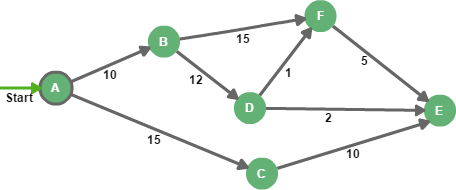
\includegraphics[width=3in]{final-exam-preparation/dijkstra-graph.png}}
\caption{\label{fig:dijkstra-graph} A weighted graph.}
\end{figure}

\begin{tabular}{|l|c|c|} \hline
Vertex & Mininum Path & Step number \\ \hline
$B$ & & \\ \hline
$C$ & & \\ \hline
$D$ & & \\ \hline
$E$ & & \\ \hline
$F$ & & \\ \hline
\end{tabular}


\end{document}




\newpage
\documentclass[jou]{apa6}

\usepackage[american]{babel}

\usepackage{csquotes}
\usepackage[style=apa,sortcites=true,sorting=nyt,backend=biber]{biblatex}
\DeclareLanguageMapping{american}{american-apa}
\addbibresource{bibliography.bib}


%%%%%%%%%%%%%%%%%%%%%%%%%%%%%%%%%%%%%%%%
%% Discrete Structures
%% The start of RBS stuff
%%%%%%%%%%%%%%%%%%%%%%%%%%%%%%%%%%%%%%%%

% Working internal and external links in PDF
\usepackage{hyperref}
% Extra math symbols in LaTeX
\usepackage{amsmath}
\usepackage{gensymb}
\usepackage{amssymb}
% Enumerations with (a), (b), etc.
\usepackage{enumerate}
\usepackage[framemethod=TikZ]{mdframed}
\usepackage{xcolor}

\let\OLDitemize\itemize
\renewcommand\itemize{\OLDitemize\addtolength{\itemsep}{-6pt}}

\usepackage{etoolbox}
\makeatletter
\preto{\@verbatim}{\topsep=3pt \partopsep=3pt }
\makeatother

% These sizes redefine APA for A4 paper size
\oddsidemargin 0.0in
\evensidemargin 0.0in
\textwidth 6.27in
\headheight 1.0in
\topmargin -24pt
\headheight 12pt
\headsep 12pt
\textheight 9.19in



\title{Sample Quiz 8}
\author{Discrete Structures, Spring 2020}
\affiliation{RBS}

\leftheader{Discrete Sample Quiz 8}

\abstract{%
}

%\keywords{}

\setlength\parindent{0pt}

\begin{document}

%\thispagestyle{empty}

\twocolumn
\section{Final Exam, 2020-04-23}

\vspace{4pt}
{\bf Question 1.}\\
By $U$ we denote the set of all positive integers 
between $1$ and $120$. This is the {\em universe} in which 
we define several subsets:
$$\left\{ \begin{array}{l}
A = \{ x \in U\;\mid\;2\mid{}x\},\\
B = \{ x \in U\;\mid\;3\mid{}x\},\\
C = \{ x \in U\;\mid\;5\mid{}x\},\\
X = \{ x \in U\;\mid\;2\mid{}x\;\vee\;3\mid{}x\},\\
Y = \{ x \in U\;\mid\;(3\mid{}x\;\wedge\;5\mid{}x)\;\vee\neg(2\mid{}x)\}.
\end{array} \right.$$

{\bf (A)} Express $X$ using the sets $A,B,C$ (using set union $V \cup W$, 
set intersection $V \cap W$, set complement $\overline{V}$ operations).\\
{\bf (B)} Express $Y$ using the sets $A,B,C$ in a similar way.\\
{\bf (C)} Find $|X|$ - the size of the set $X$.\\
{\bf (D)} Find $|Y|$ - the size of the set $Y$.




\vspace{10pt}
{\bf Question 2.}\\
Let $A$ and $B$ be sets with sizes $|A| = 8$ and $|B| = 5$
and $|A \cap B| = 3$. 

Calculate the largest and the smallest possible values 
for each of the following set sizes: 

{\bf (A)} $|A \cup B|$.\\
{\bf (B)} $|A \times (B \times B)|$.\\
{\bf (C)} $\left| \mathcal{P}(\mathcal{P}(A \cap B)) \right|$ - the 
powerset of a powerset of $A \cap B$.\\
{\bf (D)} $|A \oplus B|$ - the symmetric difference of the sets $A$ and $B$.


\vspace{10pt}
{\bf Question 3.}\\ 
Consider the following recurrent sequence: 

$$\left\{ \begin{array}{l}
a_0 = 3\\
a_1 = 4\\
a_{n+2} = 5a_{n+1} - 6a_n,\;\text{if}\;n \geq 0 \\
\end{array} \right.$$

Assume that $b_n$ is another sequence satisfying the 
recurrence rule
$$b_{n+2} = 5b_{n+1} - 6b_n,\;\text{if}\;n \geq 0$$
(The first two members $b_0,b_1$ are not known.)

{\bf (A)} Write the first $6$ members of this sequence ($a_0,\ldots,a_5$).\\
{\bf (B)} Write the characteristic equation for this sequence.\\
{\bf (C)} Write the general expression for an arbirary sequence $b_n$
satisfying the recurrent expression as a sum of two geometric progressions 
(you can leave unknown coefficients in your answer; just explain which ones they are).\\
{\bf (D)} Write the formula to compute $a_n$ (that would satisfy 
the initial conditions $a_0 = 3$ and $a_1 = 4$).


\vspace{10pt}
{\bf Question 4.}\\ 
Consider this code snippet in Python:

\begin{verbatim}
n = 1000
sum = 0
for i in range(1, n*n+1):
    for j in range(1,i+1):
        sum += i % j
\end{verbatim}

And a similar one in R:

\begin{verbatim}
n <- 1000
sum <- 0
for (i in 1:(n*n)) {
    for (j in 1:i) {
        sum <- sum + i %% j
    }
}
\end{verbatim}

{\bf (A)} Explain in human language what this algorithm does.\\
{\bf (B)} Denote by $f(n)$ the 
number of times the variable `sum` is incremented. 
Write the Big-O-Notation for $f(n)$. Find 
a function $g(n)$ such that 
$f(n)$ is in $O(g(n))$. (If there are multiple functions, 
pick the one with the slowest growth.)\\
{\bf (C)} Express the function $f(n)$ precisely - 
how many times `sum` is incremented in terms of variable $n$. 







\vspace{10pt}
{\bf Question 5.}

Let $A$ be the set of all positive divisors of the number $120$ 
(including $1$ and $120$ itself).  

{\bf (A)} What is the multiplication of all 
numbers in the set $A$?\\
{\bf (B)} Express this number as the product of prime powers.

 
 


\vspace{10pt}
{\bf Question 6.} 

Define the following binary relationship on the set of 
integer numbers $\mathbb{Z}$:   
We say that $aRb$ (numbers $a,b \in \mathbb{Z}$ are in the relation $R$) iff
$$\left\{ \begin{array}{l}
a - b \equiv 0\,(\text{mod}\;11)\\
a - b \equiv 0\,(\text{mod}\;12)\\
a - b \equiv 0\,(\text{mod}\;13)
\end{array} \right.$$

\begin{tabular}{|l|l|l|} \hline
{\bf Item} & {\bf Statement} & {\bf True or False?} \\ \hline
{\bf (A)} & $R$ is reflexive &  \\ \hline
{\bf (B)} & $R$ is symmetric &  \\ \hline
{\bf (C)} & $R$ is antisymmetric &  \\ \hline
{\bf (D)} & $R$ is transitive &  \\ \hline
{\bf (E)} & $aRb$ iff $a=b$ &  \\ \hline
\end{tabular}

For all items where you answered `FALSE`, specify a counterexample
(values for some numbers that would make the condition true, but the 
conclusion false). 
If the statement was true, write "none".


{\bf (A)} counterexample: $\ldots$\\
{\bf (B)} counterexample: $\ldots$\\
{\bf (C)} counterexample: $\ldots$\\
{\bf (D)} counterexample: $\ldots$\\
{\bf (E)} counterexample: $\ldots$


\vspace{10pt}
{\bf Question 7.}\\
Four people $A,B,C,D$ each has his own hat. 
After the meeting they leave their 
building in a hurry, everyone grabs some hat at random 
so that all $4!$ permutations of the hats have equal probabilities. 

Let the random variable $X$ denote the number of hats that
were picked up correctly. (For example, if
the hat assignment is this: $(A \rightarrow A, 
B \rightarrow B, C \rightarrow D, D \rightarrow C)$, then 
$X = 2$, because two people got their own hats.)

{\bf (A)}  Find $E(X)$ - the expected value of $X$.\\
{\bf (B)}  Find $V(X)$ - the variance of $X$. 



\vspace{10pt}
{\bf Question 8.}\\
There was a crooked man who had a crooked 1 euro coin. 
On lucky days it would flip the *heads* with probability $p=\frac{2}{3}$, 
and the *tails* with probability $p=\frac{1}{3}$, but on unlucky days
it was the opposite ($p(\mathtt{heads})=\frac{1}{3}$, but
$p(\mathtt{tails})=\frac{2}{3}$). 
There were equal probabilities of $\frac{1}{2}$ for lucky and unlucky days.


One morning he flipped the coin $5$ times and altogether got three {\em heads}
and two {\em tails}.

Let us introduce the following events:

\begin{itemize}
\item $E$ (evidence): Five coin tosses result in three {\em heads} and two {\em tails}.
\item $H$ (hypothesis): The current day is lucky.
\end{itemize}

{\bf (A)} Find $P(E|H)$ - the conditional probability of $E$ given that the 
day is lucky.\\
{\bf (B)} Find $P(E|H)\cdot P(H)$ - the probability that the day 
is lucky and $E$ happens.\\
{\bf (C)} Find $P(E|\overline{H})$ - the conditional probability of $E$
given that the day is not lucky.\\
{\bf (D)} Find $P(E|\overline{H})\cdot P(\overline{H})$ - the probability 
that the day is unlucky and $E$ happens.\\
{\bf (E)} Find $P(E)$ - as the sum of two probabilities ($E$ happened
on a lucky day and also $E$ happened on unlucky day).\\
{\bf (F)} Find the conditional probability $P(H|E)$ - 
the likelyhood that the croocked man has a lucky day, given 
that the event $E$ has happened.






\vspace{10pt}
{\bf Question 9.}

\begin{figure}[!htb]
\center{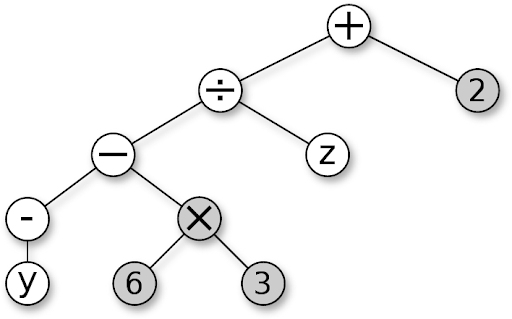
\includegraphics[width=2in]{final/final-syntax-tree.png}}
\caption{\label{fig:final-syntax-tree} A tree for an expression.}
\end{figure}

The syntax tree describes an algebraic expression (please note
the difference between the unary minus that
flips the value of the variable $y$ and 
the binary minus that subtracts the 
two subexpressions: $-y$ and $6 \times 3$). 

{\bf (A)} Write the preorder DFS traversal of
this tree.\\
{\bf (B)} Write the inorder DFS traversal of 
this tree.\\
{\bf (C)} Write the postorder DFS traversal of 
this tree.

{\em Note.} In all $3$ answers denote the unary 
minus with the tilde sign $\sim$, 
but the regular/binary minus with $-$. 






\vspace{10pt}
{\bf Question 10.}\\
\begin{figure}[!htb]
\center{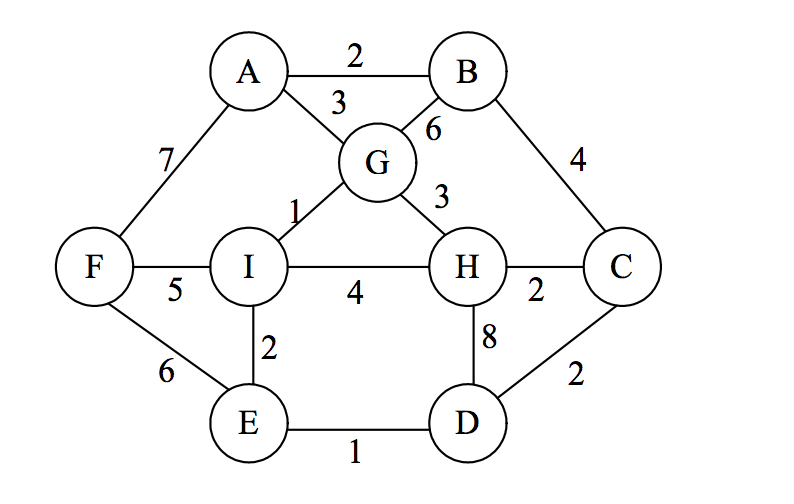
\includegraphics[width=2in]{final/prim-weighted-graph.png}}
\caption{\label{fig:prim-weighted-graph} A graph with 9 vertices.}
\end{figure}

Run the Prim's algorithm on the weighted graph in Figure~\ref{fig:prim-weighted-graph}, 
start growing the tree from the vertex $I$. 

\begin{tabular}{|l|l|} \hline
{\bf Step} & {\bf Newly Added Edge} \\ \hline
{\bf Step 1} & \\ \hline
{\bf Step 2} & \\ \hline
{\bf Step 3} & \\ \hline
{\bf Step 4} & \\ \hline
{\bf Step 5} & \\ \hline
{\bf Step 6} & \\ \hline
{\bf Step 7} & \\ \hline
{\bf Step 8} & \\ \hline
\end{tabular}


What is the total weight of the obtained Minimum Spanning Tree?





\mbox{}
\newpage
\subsection{Answers}

Every problem is worth $15$ points. The total for this final is 150 points.


\vspace{4pt}
{\bf Question 1.}\\

{\bf (A)} $X = A \cup B$ (Boolean OR means set union)\\
{\bf (B)} $Y = (B \cap C) \cup \overline{A}$ (Boolean and means set intersection; negation means set complement)\\
{\bf (C)} $|X| = |A| + |B| - |A \cap B| = 60+40-20 = 80$ (principle of inclusion-exclusion).\\
{\bf (D)} $|Y|$ is all odd numbers and also four even numbers divisible by $15$
($30, 60, 90, 120$). The total is $60 + 4 = 64$. 

{\scriptsize
{\em Grading.} 
\begin{itemize}
\item Each correct answer is $3$ points (total $12$). 
\item Explaining both {\bf (C}) and {\bf (D)} is another $3$ points (total $3$).
\item Using wrong set notation ($\wedge$ instead of $\cap$ etc.) divides the number of points in half.
\item $68$ instead of $64$ is $2$ points (instead of $3$). 
\end{itemize}
}


\vspace{10pt}
{\bf Question 2.}\\
In all the answers the largest and the smallest value are equal, because
we know exactly how the two sets intersect; how many elements belong to just
one of the sets $A$, $B$, and how many elements belong to the both sets. 

{\bf (A)} $|A \cup B| = |A| + |B| - |A \cap B| = 8+5-3 = 10$ (the principle of inclusion-exclusion).\\
{\bf (B)} $|A \times (B \times B)| = 8 \cdot 5 \cdot 5 = 200$\\
(Cartesian product has size that is the product of all participant sets: 
one can combine three elements from the sets $A$, $B$ and $B$ in this many ways).\\
{\bf (C)} $2^{2^3} = 2^8 = 256$ (the number of elements in the powerset 
of any set $X$ can be obtained by raising $2$ to the power $|X|$).\\
{\bf (D)} $|A \oplus B| = (8-3) + (5-3) = 7$ (we remove the common elements from both $A$ and $B$). 


{\scriptsize
{\em Grading.} 
\begin{itemize}
\item Each correct answer is $3$ points (total $12$).
\item Expressions or verbal explanations of the answers is $3$ points (total $3$).
\end{itemize}
}



\vspace{10pt}
{\bf Question 3.}\\
{\bf (A)} $a_0 = 3$,\\
$a_1 = 4$,\\
$a_2 = 5\cdot 4 - 6 \cdot 3 = 2$,\\
$a_3 = 5\cdot 2 - 6 \cdot 4 = -14$,\\  
$a_4 = 5\cdot(-14) - 6 \cdot 2 = -82$,\\
$a_5 = 5\cdot(-82) - 6 \cdot (-14) = -326$,\\
$a_6 = 5\cdot(-326) - 6 \cdot (-82) = -1138$.

{\bf (B)} The characteristic equation is obtained, if we try to find $a_n$ 
in the form of a geometric progression $r^n$:   
$r^{n+2} = 5r^{n+1} - 6r^n,$ or  
$r^2 -5r + 6 = 0$.   
It has two roots: $r_1 = 2$, $r_2 = 3$. 

{\bf (C)} The general form of the expression for any iterative
sequence $b_n$ satisfying the relationship $b_{n+2} = 5b_{n+1} - 6b_n$ is as follows:
$$b_n = A \cdot 2^n + B \cdot 3^n,$$
where $A,B$ are two constants that depend on the two initial values of the sequence $b_n$. 

{\bf (D)} We need to solve a system of two equations, to ensure that the formula
$a_n = A \cdot 2^n + B \cdot 3^n$ has correct values for $n=0$ and $n=1$. 
We get the following system: 
$$\left\{ \begin{array}{l} 
A + B = 3,\\
2A + 3B = 4.\\
\end{array} \right.$$
Substitute $B = 3-A$ into the second equation. We get that 
$2A + 9 - 3A = 4$ and $A = 5$. We also get that $B = -2$. 
Therefore the exact formula to calculate the sequence $a_n$ is this:
$$a_n  = 5 \cdot 2^n - 2 \cdot 3^n,\;\text{where}\;n \geq 0.$$
This actually works, if we plug in the values calculated in {\bf (A)} for $n = 0,\ldots,6$.

{\scriptsize
{\em Grading.} 
\begin{itemize}
\item Answer in {\bf (A)} is $4$ points.
\item Answer in {\bf (B)} is $4$ points.
\item Answer in {\bf (C)} is $3$ points.
\item Answer in {\bf (D)} is $4$ points.
\end{itemize}
}





\vspace{10pt}
{\bf Question 4.}\\
{\bf (A)} The algorithm takes all numbers $i$ from $1$ to $n^2$ and
divides them by all the smaller numbers $j < i$, and adds up all the obtained remainders.

{\bf (C)} The outer loop is repeated $n^2$ times. The inner loop is repeated
$1 + 2 + 3 + \ldots + n^2$ times. This is an arithmetic progression.
The sum of an arithmetic progression is the arithmetic mean of the first and the last 
member multiplied by the number of members: 
$$f(n) = \frac{1 + n^2}{2} \cdot n^2 = \frac{n^4 + n^2}{2}.$$

{\bf (B)} $f(n)$ is in $O(n^4)$. Therefore we can take $g(n) = n^4$. We can
pick another $g(n)$ that is multiplied by some nonzero constant
(such as $\frac{n^4}{2}$ or $17n^4$ or anything else - that also counts
as a valid answer).  
Certainly, $f(n)$ is also in $O(n^k)$ for any $k > 4$, but the function $g(n) = n^4$ 
is the slowest growing. 

{\scriptsize
{\em Grading.} 
\begin{itemize}
\item Answer for {\bf (A)} is $5$ points.
\item Answer for {\bf (B)} (any 4th degree polynomial of $n$) is $5$ points. 
An attempt to estimate some arithmetic progression with a different upper limit
(say, $1 + 2 + \ldots + n$) gets $2$ points.
\item Answer for {\bf (C)} is $5$ points. If the answer is 
provided just for $n=1000$ (not for any variable), then it is $4$ points.
\end{itemize}
}







\vspace{10pt}
{\bf Question 5.}\\
{\bf (A)} If expressed as a product of two positive integers $120 = ab$, 
one of the divisors $a$ or $b$ would be smaller than $\sqrt{120} \approx 11$, and the other
one would be bigger. We can easily list all the ways to express $120$ 
as a product of two integers: 
$$1 \cdot 120 = 2 \cdot 60 = 3 \cdot 40 = 4 \cdot 30 = $$
$$= 5 \cdot 24 = 6 \cdot 20 = 8 \cdot 15 = 10 \cdot 12,$$
and there are no other factorizations, since all the divisors less than $11$ are
already listed.  
Multiplying them all together would give 
$$(120)^8 = 42998169600000000$$

{\bf (B)} As a product of prime factors:
$$(120)^8 = (2^3 \cdot 3 \cdot 5)^8 = 2^{24} \cdot 3^8 \cdot 5^8.$$

{\scriptsize
{\em Grading.} 
\begin{itemize}
\item Correct item {\bf (A)} is $7$ points (also floating point answers were fine - 
not all had easy access to the big integer arithmetic). 
\item Correct item {\bf (B)} is $8$ points.
\end{itemize}
}


\vspace{10pt}
{\bf Question 6.}\\

\begin{tabular}{|l|l|l|} \hline
{\bf Item} & {\bf Statement} & {\bf True or False?} \\ \hline
{\bf (A)} & $R$ is reflexive & TRUE \\ \hline
{\bf (B)} & $R$ is symmetric & TRUE \\ \hline
{\bf (C)} & $R$ is antisymmetric & FALSE \\ \hline
{\bf (D)} & $R$ is transitive & TRUE \\ \hline
{\bf (E)} & $aRb$ iff $a=b$ & FALSE \\ \hline
\end{tabular}


{\bf (A)} Counterexample: None\\
{\bf (B)} Counterexample: None\\
{\bf (C)} Consider counterexample $a=0$, $b = 11 \cdot 12 \cdot 13 = 1716$.  
While it is true that $aRb$ and $bRa$, nevertheless $a \neq b$.\\
{\bf (D)} Counterexample: None\\
{\bf (E)} Counterexample is same as in {\bf (C)}: $a=0$, $b = 1716$.

{\scriptsize
{\em Grading.} 
\begin{itemize} 
\item One correct answer is $2$ points (total $10$).
\item Counterexamples for {\bf (C)} and {\bf (E)} is $5$ points (they are, in fact, the same). 
\end{itemize}
}



\vspace{10pt}
{\bf Question 7.} Answer: {\tt 17}\\

\begin{itemize}
\item For $1$ of $24$ permutations $X = 4$ (all hats stay in place),
\item For $0$ permutations $X = 3$ (it is not possible for exactly three hats to stay in place, because
then the 4th hat also returns to its owner),
\item For $6$ of $24$ permutations $X = 2$ (there are ${4 \choose 2} = 6$ ways how to pick $2$ hats
that stay in place; and the remaining two hats can switch places only in one way),
\item For $8$ of $24$ permutations $X = 1$ (there are ${4 \choose 1} = 4$ ways how to pick $1$ hat
that stays in place; and the remaining three hats can rotate in two ways). 
\item For the remaining $24 - (1 + 6 + 8) = 9$ permutations $X = 0$ (no hats stay in place).
\end{itemize}

{\scriptsize
\begin{table}[h!]
\begin{center}
\caption{Random Variable $X$ for the Hat Problem}
\begin{tabular}{|l|r|r|r|} \hline
\label{table:t1}
{\bf Permutation} & $X$ & $X-E(X)$ & $(X-E(X))^2$ \\ \hline
$\textcolor{red}{\mathtt{ABCD}}$ & $4$ & $3$ & $9$ \\ \hline
$\textcolor{red}{\mathtt{AB}}\mathtt{DC}$ & $2$ & $1$ & $1$ \\ \hline
$\textcolor{red}{\mathtt{A}}\mathtt{CB}\textcolor{red}{\mathtt{D}}$ & $2$ & $1$ & $1$ \\ \hline
$\textcolor{red}{\mathtt{A}}\mathtt{CDB}$ & $1$ & $0$ & $0$ \\ \hline
$\textcolor{red}{\mathtt{A}}\mathtt{DBC}$ & $1$ & $0$ & $0$ \\ \hline
$\textcolor{red}{\mathtt{A}}\mathtt{D}\textcolor{red}{\mathtt{C}}\mathtt{D}$ & $2$ & $1$ & $1$ \\ \hline

{\tt BACD} & $2$ & $1$ & $1$ \\ \hline
{\tt BADC} & $0$ & $-1$ & $1$ \\ \hline
{\tt BCAD} & $1$ & $0$ & $0$ \\ \hline
{\tt BCDA} & $0$ & $-1$ & $1$ \\ \hline
{\tt BDAC} & $0$ & $-1$ & $1$ \\ \hline
{\tt BDCA} & $1$ & $0$ & $0$ \\ \hline

{\tt CABD} & $1$ & $0$ & $0$ \\ \hline
{\tt CADB} & $0$ & $-1$ & $1$ \\ \hline
{\tt CBAD} & $2$ & $1$ & $1$ \\ \hline
{\tt CBDA} & $1$ & $0$ & $0$ \\ \hline
{\tt CDAB} & $0$ & $-1$ & $1$ \\ \hline
{\tt CDBA} & $0$ & $-1$ & $1$ \\ \hline

{\tt DABC} & $0$ & $-1$ & $1$ \\ \hline
{\tt DACB} & $1$ & $0$ & $0$ \\ \hline
{\tt DBAC} & $1$ & $0$ & $0$ \\ \hline
{\tt DBCA} & $2$ & $1$ & $1$ \\ \hline
{\tt DCAB} & $0$ & $-1$ & $1$ \\ \hline
{\tt DCBA} & $0$ & $-1$ & $1$ \\ \hline\hline
{\bf Mean} & $1$ & $0$ & $1$ \\ \hline
\end{tabular}
\end{center}
\end{table}
}





{\bf (A)} $E(X) = \frac{1}{24} \cdot 4 + \frac{6}{24} \cdot 2 + \frac{8}{24} \cdot 1 = 1$. 
This means that the expected number of hats that stay in place is exactly $1$.\\
{\bf (B)} For all $24$ permutations, subtract the value $E(X) = 1$ from 
every hat experiment outcome. Define $x_1,\ldots,x_{24}$ - all $24$ values of the 
random variable $X$ (exactly one value is $4$, exactly six values are $2$, 
exactly $8$ values are $1$, exactly $9$ values are $0$): 
$$V(X) = \frac{\sum_{i=1}^{24} (x_i - 1)^2}{24} = \frac{24}{24} = 1.$$

Therefore, $V(X) = 1$ (variance also equals $1$, but the unit of measurement 
is not hats but ``hats squared'').

{\em Note.} $E(X)=1$ is the arithmetic mean over the column $X$, but $V(X)=1$ 
is the arithmetic mean over the column $(X-E(X))^2$ (see Table~\ref{table:t1}).

{\scriptsize
{\em Grading (theoretically max=20, but most results are not that high).} 
\begin{itemize} 
\item Correctly found $E(X)$ is $5$ point.
\item Correctly found $V(X)$ is $5$ point.
\item Justified computation for $E(X)$ is $5$ points.
\item Justified computation for $V(X)$ is $5$ points.
\end{itemize}
}




\vspace{10pt}
{\bf Question 8.} \\

{\bf (A)} $P(E|H)$ is the outcome of the Binomial distribution: 
There are $n=5$ coin-toss experiments; the probability of success for any single experiment 
is $p = \frac{2}{3}$ (since we know that the day is lucky and hypothesis $H$ holds). 
Therefore, 
$$P(E|H) = {5 \choose 3} p^3 (1-p)^2 = 10 \left( \frac{2}{3} \right)^3 \left( \frac{1}{3} \right)^2 = 
\frac{80}{243}$$

{\bf (B)} $P(E|H)\cdot P(H) = \frac{80}{243}\cdot\frac{1}{2}= \frac{40}{243}$, 
since $P(H) = \frac{1}{2}$ (the {\em a priori} probability of a lucky day is exactly $1/2$). 

{\bf (C)} $P(E|\overline{H})$ is the outcome of the Binomial distribution: 
Again, there are $n=5$ coin-toss experiments, but now the probability of a single
experiment is just $p = \frac{1}{3}$. Therefore, 
$$P(E|\overline{H}) = {5 \choose 3} p^3 (1-p)^2 = 10 \left( \frac{1}{3} \right)^3 \left( \frac{2}{3} \right)^2 = 
\frac{40}{243}$$

{\bf (D)} $P(E|\overline{H}) \cdot P(\overline{H}) = \frac{40}{243}\cdot\frac{1}{2} = \frac{20}{243}$. 

{\bf (E)} We can compute $P(E)$ as the sum of two mutually incompatible events: 
event $E$ can happen either on a lucky day or on an unlucky day: 
$$P(E) = P(E|H)\cdot P(H) + P(E|\overline{H}) \cdot P(\overline{H}) = 
\frac{40}{243} + \frac{20}{243} = \frac{60}{243}.$$

{\bf (F)} Use Bayes formula: 
\begin{align}
P(H|E) = & \frac{P(E|H) \cdot P(H)}{P(E|H) \cdot P(H) + P(E|\overline{H}) \cdot P(\overline{H})} = \nonumber \\
 = & \frac{P(E|H) \cdot P(H)}{P(E)} =  \frac{ \frac{40}{243}}{ \frac{60}{243}} = \frac{2}{3}. \nonumber
\end{align}

Bayes formula is intuitive: It shows the proportion of the 
subcase $P(E|H) \cdot P(H)$ (i.e. event $E$ hapens on a lucky day) out of the
whole probability $P(E) = P(E|H)\cdot P(H) + P(E|\overline{H}) \cdot P(\overline{H})$
(i.e. event $E$ happens either on a lucky or unlucky day). 

{\scriptsize
{\em Grading (theoretically max=20, but most results are not that high).} 
\begin{itemize} 
\item Any item from {\bf (A)} to {\bf (E)} is $3$ points. 
\item Bayes formula or a similar expression finding the reverse conditional probability 
in {\bf (F)} in $5$ points.
\end{itemize}
}



\vspace{10pt}
{\bf Question 9.}\\
{\bf (A)} $\mathtt{+:-\sim{}y\times6\;3\;z\;2}$,\\
{\bf (B)} $\mathtt{y\sim{}-\,6\,\times3:z\,+\,2}$,\\
{\bf (C)} $\mathtt{y\sim{}6\;3\,\times-\,z\,:2\,+}$.

{\bf Note.} In inorder traversal {\bf (B)} we first visit 
the first subtree (e.g., $\mathtt{y}$), and only then the 
parent node (e.g., unary minus $\sim$). 
See (Rosen2019, p.811).


{\scriptsize
{\em Grading.} 
\begin{itemize}
\item Each correctly written expression is 
\item Item {\bf (B)} with switched order of the unary minus and its child node $y$ is
$3$ points instead of $5$.
\item Minor typos in single characters get $4$ or $5$ points.
\item Any major differences from the correct result do not get points.
\end{itemize}
}


%\vspace{10pt}
\newpage
{\bf Question 10.}\\

We start from vertex $I$. At every step we 
grow the tree by a single edge (so that it stays connected
and the newly added edge has the smallest possible weight). 


\begin{tabular}{|l|l|} \hline
{\bf Step} & {\bf Newly Added Edge} \\ \hline
{\bf Step 1} & $IG$, $w=1$ \\ \hline
{\bf Step 2} & $IE$, $w=2$ \\ \hline
{\bf Step 3} & $ED$, $w=1$ \\ \hline
{\bf Step 4} & $DC$, $w=2$ \\ \hline
{\bf Step 5} & $CH$, $w=2$ \\ \hline
{\bf Step 6} & $GA$, $w=3$ \\ \hline
{\bf Step 7} & $AB$, $w=2$ \\ \hline
{\bf Step 8} & $IF$, $w=5$ \\ \hline
\end{tabular}


The total weight of all added edges (same as the total weight of the MST) is $18$. 


\begin{figure}[!htb]
\center{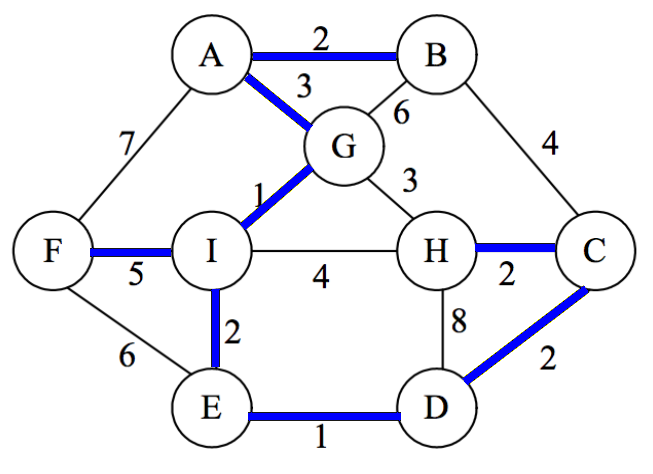
\includegraphics[width=1.5in]{final/prim-weighted-mst.png}}
\caption{\label{fig:prim-weighted-mst} MST edges shown in blue.}
\end{figure}

{\scriptsize
{\em Grading.} 
\begin{itemize}
\item Incorrectly adding up weights could subtract $1$ or $2$ points from the total.
\item Adding $9$ edge weights (or any other number instead of $8$ weights) and getting incorrect sum is $11$ points (instead of $15$). 
\item Not showing the edges in answers (or displaying them in an order that differs from Prim's algorithm), 
but still getting something close to MST is about $8$ points.
\end{itemize}
}


\end{document}




\newpage
\documentclass[jou]{apa6}

\usepackage[american]{babel}

\usepackage{csquotes}
\usepackage[style=apa,sortcites=true,sorting=nyt,backend=biber]{biblatex}
\DeclareLanguageMapping{american}{american-apa}
\addbibresource{bibliography.bib}


%%%%%%%%%%%%%%%%%%%%%%%%%%%%%%%%%%%%%%%%
%% Discrete Structures
%% The start of RBS stuff
%%%%%%%%%%%%%%%%%%%%%%%%%%%%%%%%%%%%%%%%

% Working internal and external links in PDF
\usepackage{hyperref}
% Extra math symbols in LaTeX
\usepackage{amsmath}
\usepackage{gensymb}
\usepackage{amssymb}
% Enumerations with (a), (b), etc.
\usepackage{enumerate}
\usepackage[framemethod=TikZ]{mdframed}
\usepackage{xcolor}
\usepackage{graphicx}
\usepackage[justification=centering]{caption}
\usepackage{fancyvrb}

\let\OLDitemize\itemize
\renewcommand\itemize{\OLDitemize\addtolength{\itemsep}{-6pt}}

\usepackage{etoolbox}
\makeatletter
\preto{\@verbatim}{\topsep=3pt \partopsep=3pt }
\makeatother

% These sizes redefine APA for A4 paper size
\oddsidemargin 0.0in
\evensidemargin 0.0in
\textwidth 6.27in
\headheight 1.0in
%\topmargin -24pt
\topmargin -32pt
\headheight 12pt
\headsep 12pt
%\textheight 9.19in
\textheight 9.35in


\title{Sample Quiz 8}
\author{Discrete Structures, Spring 2020}
\affiliation{RBS}

\leftheader{Discrete Sample Quiz 8}

\abstract{%
}

%\keywords{}

\setlength\parindent{0pt}

\begin{document}

\twocolumn

\section{Appendix: Quiz on Individual Topics}

\vspace{4pt}
{\bf Question 1.} A hacker wants to 
use {\em Arithmetic coding}
that would send a virus to the client's computer and unpack itself there.
His favorite virus uses this RNS sequence: $\textcolor{blue}{\mathtt{GACGU\$}}$, 
where $\textcolor{blue}{\mathtt{A}},\textcolor{blue}{\mathtt{C}},\textcolor{blue}{\mathtt{G}},\textcolor{blue}{\mathtt{U}}$ are four nucleobases (the useful data payload), 
but the symbol $\textcolor{blue}{\$}$ is used just once to mark 
the end of the RNS string. 

He uses the following {\em a priori} frequencies for the symbols: 

\begin{tabular}{ccccc}
$\textcolor{blue}{\mathtt{A}}$ & $\textcolor{blue}{\mathtt{C}}$ & $\textcolor{blue}{\mathtt{G}}$ & $\textcolor{blue}{\mathtt{U}}$ & $\textcolor{blue}{\mathtt{\$}}$ \\ 
$30\%$ & $10\%$ & $30\%$ & $20\%$ & $10\%$ \\
\end{tabular}


\vspace{4pt}
He starts with the half-closed line segment $S_0 = [0;1)$ and at every step (for all $i = 0,1,2,3,4,5$) creates the 
next segment $S_{i+1}$ from $S_i$ by dividing $S_i$ into five parts of lengths proportional 
to the frequencies (the proportions of subdivisions are $3\!\!:\!\!1\!\!:\!\!3\!\!:\!\!2\!\!:\!\!1$). Then $S_{i+1}$ is the
subdivision of the previous $S_i$ corresponding to the newly encoded character.
After encoding all six characters in the virus message $\textcolor{blue}{\mathtt{GACGU\$}}$, the hacker
gets the segment $S_6$.

\begin{figure}[!htb]
\center{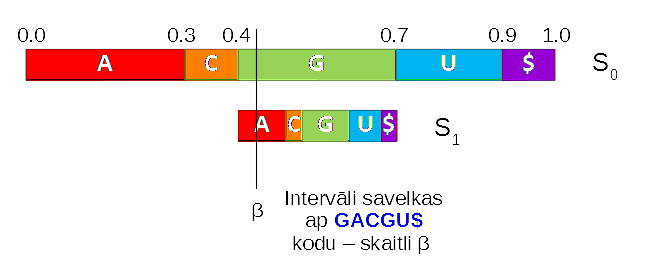
\includegraphics[width=3in]{quiz-on-individual-topics/arithmetic-coding.png}}
\caption{\label{fig:arithmetic-coding} Building arithmetic code}
\end{figure}


Find the binary fraction $\beta$ belonging to $S_6$.\\
\textcolor{teal}{\em Select one answer.}

{\bf (A)} $\beta = 0.011011101100011_2$\\
{\bf (B)} $\beta = 0.011011101100110_2$\\
{\bf (C)} $\beta = 0.011011101101001_2$\\
{\bf (D)} $\beta = 0.011011101101100_2$\\
{\bf (E)} $\beta = 0.011011101101111_2$\\


{\em Note.} In arithmetic coding any sequence of 
$n$ bits represents an interval of length $\frac{1}{2^n}$.
For example the bit sequence {\tt 010} stands for the segment of real numbers:
$[0.010_2; 0.011_2) = [0.25; 0.375)$ having length $\frac{1}{2^3} = \frac{1}{8}$. 
If the arithmetic coding yields a segment $[a;b)$ such that 
$[0.25; 0.375) \subseteq [a;b)$, then {\tt 010} is the 
result of the arithmetic coding.

The number $\beta = 0.010_2 \in [a;b)$, and the extra "0"
character ensures that the interval is not too long and it fits inside $[a;b)$. 
For example, {\tt 01} would represent a different interval $[0.25; 0.5) \neq [0.25; 0.375)$. 


\vspace{10pt}
{\bf Question 2.} We want to use a {\em regular expression} 
to find all phone numbers with the Latvian country code.
Assume that the phones can have one of the following formats (here 
symbol {\tt D} denotes any digit (0-9)). The space symbols
are used exactly as written (they are single space characters).

\begin{verbatim}
(+371) DDDDDDDD
+371 DDDDDDDD
\end{verbatim}

Pick a regular expression that would recognize just these 2 phone formats.\\
\textcolor{teal}{\em Select one answer.}


\begin{verbatim}
(A)   (+371|\(+371\)) \d{8}
(B)   (\+371|\(\+371\)) [0-9]{8}
(C)   (+371|\(+371\)) \d\d\d\d\d\d\d\d
(D)   \+371|(\+371\) [0-9]{8,8}
\end{verbatim}


{\em Note.} If you wish, you can use text editor such as Notepad++ search dialogue 
to verify which regex works. (Click {\bf Ctrl+F}, 
enter your regular expression, switch ``Search mode'' to Regular Expression, 
and click the button  ``Find All in All Opened Documents''): 


\begin{figure}[!htb]
\center{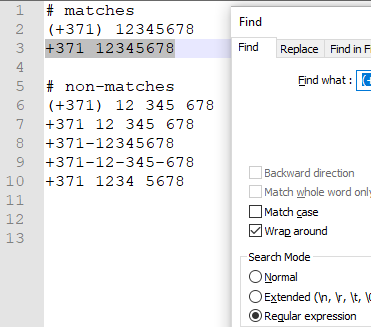
\includegraphics[width=2in]{quiz-on-individual-topics/notepad-regex.png}}
\caption{\label{fig:regex-search} Regex Search in Notepad++}
\end{figure}

If you are on a Linux machine, you can also 
test regex search with the command "grep" (and flag -E). 


\vspace{10pt}
{\bf Question 3.} About 70\% of the entries in a bit array of a {\em Bloom filter} are 
equal to $1$ as it is initialized with the words 
from some dictionary $D$. 
The Bloom filter computes $n=8$ independent hash functions to check, 
if some entry belongs to the dictionary $D$. 
What is an (approximate) chance $P$ to get a false positive?
A false positive is an event where one picks 
a random word $w \not\in D$,
and Bloom filter incorrectly states that $w$ belongs to $D$\\

\vspace{4pt}
\textcolor{teal}{\em Select one answer.}\\
{\bf (A)} $P = 30.00\%$,\\
{\bf (B)} $P = 5.76\%$,\\
{\bf (C)} $P = 3.75\%$,\\
{\bf (D)} $P = 0.66\%$.



\vspace{10pt}
{\bf Question 4.} 
A testing laboratory tests the same number of people daily, and on day $i$, the number
of people who tested positively for some health condition was $n_i$. The laboratory knows that 
the numbers $n_i$ are distributed according to {\em Poisson distribution} with the 
expected value $\lambda = 13.5$. 

By $P$ we denote the probability that on the given day 
$n_i < 5$ (i.e. less than $5$ people test 
positive for that condition). Which is the closest approximate value for this probability? 

{\bf (A)} $P = 0.26\%$,\\
{\bf (B)} $P = 0.51\%$,\\
{\bf (C)} $P = 5.78\%$,\\
{\bf (D)} $P = 10.89\%$.

{\em Note.} Another typical illustration of the same Poisson distribution: 
Imagine the ice cream ``R\={u}jienas sald\={e}jums'' with raisins. (In this case
the average number of raisins in one package is $\lambda = 13.5$; and you have to find the 
probability that a given ice cream package has at most $4$ raisins. 
See \url{https://bit.ly/2KanwIf}. 

\begin{figure}[!htb]
\center{
\includegraphics[width=1in]{quiz-on-individual-topics/rujiena-icecream.png}}
\caption{\label{fig:rujiena-icecream} An Ice Cream Package with Raisins satisfying Poisson Distribution}
\end{figure}


% ff <- function(k) {  return((lam^k*exp(-lam))/factorial(k) }

\vspace{10pt}
{\bf Question 5.} Find the minimum number of colors to paint the $12$ vertices
from the graph shown in Figure~\ref{fig:graph-coloring} so
that any two vertices connected with an edge are having different colors. 
(This number $n$ is called the {\em chromatic number} for the graph $G$.)

\begin{figure}[!htb]
\center{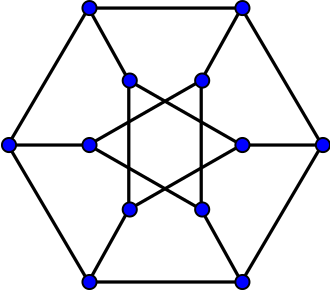
\includegraphics[width=1.6in]{quiz-on-individual-topics/durer-graph.png}}
\caption{\label{fig:graph-coloring} Graph for Vertex Coloring}
\end{figure}




\vspace{10pt}
{\bf Question 6.} Assume that the ``World Wide Web'' contains only 
$4$ pages $A,B,C,D$ that link to each other as shown in the picture below.


\begin{figure}[!htb]
\center{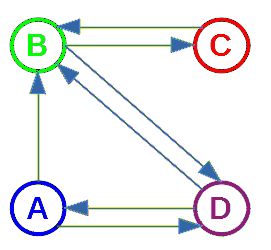
\includegraphics[width=1in]{quiz-on-individual-topics/pageranks.png}}
\caption{\label{fig:pageranks} Four webpages with links.}
\end{figure}


% https://matrix.reshish.com/multiplication.php

In the Iteration $0$ initialize the page ranks with equal values 
$$\text{PR}_0(A) = \ldots = \text{PR}_0(D) = \frac{1}{4}.$$ 
Compute the first two iterations of these pageranks, using the formulas: 
$$\left\{ \begin{array}{l}
\text{PR}_{i+1}(A) = (1 - d) + d\left( \frac{\text{PR}_i(D)}{2} \right)\\
\text{PR}_{i+1}(B) = (1 - d) + d\left( \frac{\text{PR}_i(A)}{2} + \frac{\text{PR}_i(C)}{1} + \frac{\text{PR}_i(D)}{2}  \right)\\
\text{PR}_{i+1}(C) = (1 - d) + d\left( \frac{\text{PR}_i(B)}{2} \right)\\
\text{PR}_{i+1}(D) = (1 - d) + d\left( \frac{\text{PR}_i(A)}{2} + \frac{\text{PR}_i(B)}{2} \right)
\end{array} \right.$$
Set the value of the damping factor $d=0$.

Write the values of the second iteration for all the pages:
$\text{PR}_2(A),\ldots,\text{PR}_2(D).$.

\textcolor{teal}{\em Write $4$ comma-separated numbers; round them to 
the nearest thousandth.}





\vspace{4pt}
{\em Note.} You can also use vector algebra, if you are 
familiar with multiplying matrices with vectors
\textendash{} \url{https://bit.ly/2RJTNtC}.
$$\left( \begin{array}{c}
\text{PR}_2(A)\\
\text{PR}_2(B)\\
\text{PR}_2(C)\\
\text{PR}_2(D)
\end{array} \right) = \left( 
\begin{array}{cccc}
\textcolor{blue}{0}   & \textcolor{green}{0}   & \textcolor{red}{0} & \textcolor{purple}{1/2} \\
\textcolor{blue}{1/2} & \textcolor{green}{0}   & \textcolor{red}{1} & \textcolor{purple}{1/2} \\
\textcolor{blue}{0}   & \textcolor{green}{1/2} & \textcolor{red}{0} & \textcolor{purple}{0} \\
\textcolor{blue}{1/2} & \textcolor{green}{1/2} & \textcolor{red}{0} & \textcolor{purple}{0}
\end{array} \right)^2 \cdot \left( \begin{array}{c}
1/4 \\
1/4 \\
1/4 \\
1/4
\end{array} \right).$$
In this formula a square matrix $4 \times 4$ is twice multiplied to a $4 \times 1$
vector $(1/4, 1/4, 1/4, 1/4)$ from the left side. 
%See \url{https://bit.ly/2VkZHnh}. 


\vspace{4pt}
{\em Note.} \url{https://checkpagerank.net/check-page-rank.php}
shows that:\\
{\tt https://www.bitl.lv/} has PageRank $2/10$,\\
{\tt https://www.delfi.lv/} has PageRank $6/10$.\\
This does {\bf not} mean that there are three times more 
inbound links to Delfi than to BITL (or that these links are three times more ``valuable''). 
The value returned by this web resource is a {\em logarithmic measure}
of its iterative value. In fact, the difference between $2/10$ and $6/10$
means that the popularity of these pages differs by many orders of magnitude. 
See \url{https://bit.ly/2yrRMf7}.


\vspace{10pt}
{\bf Question 7.} As you probably know, {\em Karatsuba's algorithm} can express 
the multiplication of two numbers of length $n$ digits as 
three multiplications of numbers of length $n/2$ (i.e. the number of 
operations are three times larger, but the operands become two times shorter). 
This ultimately means that Karatsuba's algorithm requires
only $O(n^{1.585})$ operations to multiply numbers of length $n$.

Imagine that somebody has invented a new operation $a \otimes b$ for 
some objects $a,b$ (both $a,b$ have the same size $n$). 
Assume that s/he knows how to express 
$a \otimes b$ using $7$ operations $a_i \otimes b_i$ (where $i = 1,2,\ldots,7$, and
all $a_i,b_i$ have size $n/2$, i.e. half the size of the original operands $a,b$). 
({\em We do not care, what the operation $\otimes$ does; but we know that we 
can compute it for arguments $a,b$ of length $1$ in constant time; it is 
therefore easy for very short arguments.})

Find the best Big-O-Notation estimate for the time needed to compute $a \otimes b$, if $a,b$ are
both of size $n$. 

{\bf (A)} $O(n^2)$\\
{\bf (B)} $O(n^2 \log n)$\\
{\bf (C)} $O(n^{2.646})$\\
{\bf (D)} $O(n^{2.808})$\\
{\bf (E)} $O(n^3)$\\
{\bf (F)} $O(n^3 \log n)$\\
\textcolor{teal}{\em Select one answer.}

\vspace{4pt}
{\em Note 1.} One can use Master's theorem (Rosen2019, p.558) for 
this problem and also for the Karatsuba's algorithm.

\vspace{4pt}
{\em Note 2.} If the algorithm falls in multiple Big-O complexity classes, pick 
the one that shows the slowest growth. For example, if a speed of an algorithm is 
both in $O(n^2)$ and $O(n^3)$, 
then $O(n^2)$ would be a more precise and a more useful estimate.


\vspace{10pt}
{\bf Question 8.} Assume that two players $A$ and $B$ play a {\em matrix game}. 
They simultaneously guess one number each. Either player can guess 
one of these three numbers: $\{ 1,2,5 \}$. 
The payoff matrix is shown below. 
In each cell the first number is what is paid to player $A$, 
the second number is paid to player $B$. 

\begin{figure}[!htb]
\center{\includegraphics[width=2.4in]{quiz-on-individual-topics/matrix-game.png}}
\caption{\label{fig:matrix-game} Matrix game with payoffs.}
\end{figure}

Expressed in human language, the rules are as follows. 
Assume that the player $A$ just guessed a number $a$, and player $B$ guessed 
a number $b$. 
\begin{itemize}
\item If $a=b$, then it is a tie; nobody pays anything.
\item If $a>b$ (yet $a < 3b$), then $B$ pays to $A$ one euro. (And also, 
if $b>a$ yet $b < 3a$, then $A$ pays to $B$ one euro.)
\item If $a \geq 3b$, then $A$ pays to $B$ two euros. (And also, if $b \geq 3a$, 
then $B$ pays to $A$ two euros.)
\end{itemize}

{\em In this number guessing game one can win by guessing a number which is a little
bit larger than the other player's number. But one should not guess a number which is 
larger than the other by ``a lot'' (if you exceed the other player's number
three times or more, then you suffer a double loss.).}

Which can be {\em Nash equilibrium} for this number guessing game?
(You can assume that one of the answer variants is correct \textendash{} 
the same optimal strategy for both players. It is enough to find the 
one that beats all the other strategies.) 
Each strategy lists the probabilities for guessing the number $x$: 

{\bf (A)} $P(x = 1) = 1/3$, $P(x = 2) = 1/3$, $P(x = 5) = 1/3$.\\
{\bf (B)} $P(x = 1) = 0$, $P(x = 2) = 1/2$, $P(x = 5) = 1/2$.\\
{\bf (C)} $P(x = 1) = 1/2$, $P(x = 2) = 1/2$, $P(x = 5) = 0$.\\
{\bf (D)} $P(x = 1) = 1/4$, $P(x = 2) = 1/2$, $P(x = 5) = 1/4$.\\
{\bf (E)} $P(x = 1) = 2/6$, $P(x = 2) = 3/6$, $P(x = 5) = 1/6$.\\
\textcolor{teal}{\em Select one answer.}


\vspace{10pt}
{\bf Question 9.} The first iterations using Lindermayer system are given:\\
{\bf Iteration 0:} {\tt A}\\
{\bf Iteration 1:} {\tt AB}\\
{\bf Iteration 2:} {\tt ABBA}\\
{\bf Iteration 3:} {\tt ABBABAAB}\\
{\bf Iteration 4:} {\tt ABBABAABBAABABBA}

({\em To get Iteration 5: Take Iteration 4, 
change all A's into B's and
vice versa, and append such string to the end of Iteration 4.})
Find the correct set of rules to generate this L-system. 

{\bf (A)} ${\displaystyle \left\{ \begin{array}{l}
\mathtt{A} \rightarrow \mathtt{B}\\
\mathtt{B} \rightarrow \mathtt{BA}
\end{array} \right. }$\\
{\bf (B)} ${\displaystyle \left\{ \begin{array}{l}
\mathtt{A} \rightarrow \mathtt{AB}\\
\mathtt{B} \rightarrow \mathtt{AA}
\end{array} \right. }$\\
{\bf (C)} ${\displaystyle \left\{ \begin{array}{l}
\mathtt{A} \rightarrow \mathtt{AB}\\
\mathtt{B} \rightarrow \mathtt{BA}
\end{array} \right. }$\\
{\bf (D)} ${\displaystyle \left\{ \begin{array}{l}
\mathtt{A} \rightarrow \mathtt{AB}\\
\mathtt{B} \rightarrow \mathtt{AB}
\end{array} \right. }$

\textcolor{teal}{\em Select one answer.}

{\em Note.} We can have a {\em turtle} that reads this 
sequence and performs actions:
\begin{itemize}
\item Letter $\mathtt{A}$: Step $1$ unit ahead, turn 
$60^{\circ}$ counterclockwise.
\item Letter $\mathtt{B}$: Turn $180^{\circ}$. 
\end{itemize}
In this case the iterations $0,2,4,\ldots$ would produce
a fragment of Koch snowflake (Figure~\ref{fig:lindenmayer-system}).

\begin{figure}[!htb]
\center{\includegraphics[width=2.5in]{quiz-on-individual-topics/lindenmayer-system.png}}
\caption{\label{fig:lindenmayer-system} Koch curve as an L-system}
\end{figure}





\vspace{10pt}
{\bf Question 10.} Assume that someone uses
a {\em secure hash} algorithm $h(x)$ that for any file $x$
outputs a hash value consisting of exactly $100$
bits. (The typical SHA-256 algorithm would return $256$ bits.)

Assume that we want to use brute force to find 
hash collision \textendash{} two different files $x_1,x_2$
such that $h(x_1) = h(x_2)$. 
You can estimate, how many hash values we need to compute before we 
get at least $50\%$ probability to find a hash collision. 
Estimation can be done using Square aproximation from 
the Birthday paradox: 
\begin{equation}
\label{eq:square-approximation}
p_{\text{collision}} \approx \frac{n^2}{2m},
\end{equation}
Formally: If a hash function $h(x)$ can take $m$ different values and
we randomly pick $n$ different integer numbers $x_1,\ldots,x_n$, then the probability 
that there is at least one collision ($h(x_i) = h(x_j)$ and $x_i \neq x_j$) is approximately expressed by
the formula (\ref{eq:square-approximation}). See \url{https://bit.ly/2RNjhGB}.

Assume that a single hash value $h(x)$ can be computed in one microsecond
($1\,\mu{}s = 10^{-6}\,s$). Estimate the number of years it would take to produce a
collision for a 100-bit secure hash algorithm with probability at least $50\%$. 

{\bf (A)} The expected time is $0.11$ years.\\
{\bf (B)} The expected time is $35.7$ years.\\
{\bf (C)} The expected time is $71.4$ years.\\
{\bf (D)} The expected time is $856$ years.\\
{\bf (E)} The expected time is $4.02\cdot 10^{16}$ years.\\
\textcolor{teal}{\em Select one answer.}


\vspace{10pt}
{\bf Question 11.} Consider the following 
problem solving strategies: 

{\footnotesize
{\bf (A)} {\bf Drawing a picture.} Can you 
write down all the things you need to consider on paper? 
Can you order them nicely in a list or a table? 
Can you show them in a two-dimensional or a three-dimensional drawing?\\
{\bf (B)} {\bf Getting hands dirty.} Can you start experimenting with the 
problem, plug in specific values, see where they lead you?\\
{\bf (C)} {\bf Going to the extremes.} Can you pick some ``borderline case''?
Is there the smallest or the largest item that is possible in the problem?\\
{\bf (D)} {\bf Lateral thinking.} Could it happen that your current solving approach 
is not applicable or is too inefficient? Can you pretend that you 
have not spent many years studying mathematics at school; 
can you apply lateral/divergent thinking out of the box to 
come up with something unexpected?\\
{\bf (E)} {\bf Looking for symmetries.} Can we switch two numbers or two letters in our 
notation? Can we inspect just one item and notice that many others are identical?\\
{\bf (F)} {\bf Making it easier.} Can we make a simpler version of this problem and
solve it first? Insert a smaller number? Solve only one particular case of it?\\
{\bf (G)} {\bf Penultimate step.} What precondition must take place before 
the final solution step is possible? Imagine, which result you would need 
in order to say that you are ``almost done''.\\
{\bf (H)} {\bf Wishful thinking.} Can you apply some outrageous simplification to your 
initial problem. Imagine for a while that you have already solved it: What would that imply?
% http://courses.cs.vt.edu/~cs4104/shaffer/Fall2010/PSintro.pdf
}

Now consider the following problem:

\begin{figure}[!htb]
\center{\includegraphics[width=2in]{quiz-on-individual-topics/tower-of-hanoi.png}}
\caption{\label{fig:tower-of-hanoi} Tower of Hanoi}
\end{figure}

\begin{mdframed}[roundcorner=6pt]
{\footnotesize
{\bf Problem.} A Tower of Hanoi (Figure~\ref{fig:tower-of-hanoi}) 
has three pegs ($A$, $B$, $C$) and
four disks initially on the peg $A$. The task is to move all the four disks to the peg $B$, where
the following rules apply:\\
Rule 1: Only one disk can be moved at a time.\\
Rule 2: Each move consists of taking the upper disk from any peg and moving it to 
another peg.\\
Rule 3: No larger disk may be placed on top of a smaller disk.

{\em The solver wants to come up with the sequence of moves. S/he has tried
a similar game with just three disks with some trial and error, but 
is not sure how to proceed in the case with four disks. Somebody suggests 
a few ``natural looking'' hints.}

{\bf Hint 1.} Find the disk that is the hardest to move anywhere or moved least frequently?\\
{\bf Hint 2.} To which peg all the other disks need to go before we move this disk?\\
{\bf Hint 3.} Assume that you know how to move three disks from the peg $A$ to the peg $B$. 
Can you move them between any other pegs? How?
}
\end{mdframed}


What kind of problem solving strategies are contained in the hints?

\textcolor{teal}{\em Select up to three relevant strategies (A-H).}



\begin{center}
\includegraphics[width=2in]{quiz-on-individual-topics/thinking-outside-the-box.png}\\
\textcopyright{} {\em Leo Cullum}, \url{https://www.newyorker.com/}
\end{center}

\vspace{10pt}
{\bf Question 12.} Someone wants to compute a MD5 checksum for the following file: 

\textcolor{blue}{
{\tt 95.211.48.179~~~bitl.lv}
}

The following is true: 
\begin{itemize}
\item File {\tt hosts.txt} is exactly $23$ bytes long.
\item The IP address is seperated from {\tt bitl.lv} by 
a single horizontal tab (byte in hexadecimal: {\tt 0x09}). 
\item The only line is ends with a Windows-style line ending (carriage return, line feed: 
bytes in hexadecimal: {\tt 0x0D}, {\tt 0x0A}). 
\end{itemize}

Figure~\ref{fig:hosts-file} shows file displayed by {\em Total Commander}; 
button {\bf F3}, then menu item {\bf Options $>$ Hex} (and also in the Notepad++ editor).

\begin{figure}[!htb]
\center{\includegraphics[width=3in]{quiz-on-individual-topics/hosts-file.png}}
\caption{\label{fig:hosts-file} Bytes in file {\tt hosts.txt}}
\end{figure}

\textcolor{teal}{\em Copy the whole MD5 checksum in your answer.}

{\em Note.} In this exercise it is important to have exactly the
same file content as shown in the picture. 
For example, replacing the {\bf TAB} character
by one or more spaces (or Windows-style line ending with a UNIX-style
line ending) would totally change MD5. 
(For secure hashes there is absolutely no string tokenization \textendash{}
unlike plagiarism detection they are very sensitive against
the smallest changes in their input.)


\vspace{10pt}
{\bf Question 13.} There are two people playing a game: Player $A$ (he is the Maximizer \textendash{} wants
to go down to a leaf with maximum payoff), and Player $B$ (he is the Minimizer \textendash{} wants
to minimize the $A$'s payoff). The current position is the root of the tree (Figure~\ref{fig:minimax}) and it is Player's $A$
turn to make the first move (to any of the root's children). After that Player $B$ moves (going down one more level) and so on
\textendash{} until they reach a leaf, which shows the payoff for Player $A$.\\
Find the maximum payoff for Player $A$ (you could use minimax algorithm with or without Alpha-Beta pruning 
speedup to find out). 

\textcolor{teal}{\em Write the payoff as a positive integer.}

\begin{figure}[!htb]
\center{\includegraphics[width=3in]{quiz-on-individual-topics/minimax.png}}
\caption{\label{fig:minimax} Game positions in a tree.}
\end{figure}


\vspace{10pt} 
{\bf Question 14.} If you verify the Conway's game of life the configuration $P_0$ 
of a straight line with $4$ live cells (Figure~\ref{fig:conway}), 
you need $N = 2$ steps until you reach ``periodic state'' $P_2$ that will 
return after period $T = 1$ (i.e.\ returning needs just one step $P_3 = P_2$, 
since ``beehive'' configuration is stable). So in this case $(N,T)=(2,1)$ \textendash{}
there are $N=2$ preliminary steps, and after that there is a period of length $T=1$. 

\begin{figure}[!htb]
\center{\includegraphics[width=2.2in]{quiz-on-individual-topics/conway.png}}
\caption{\label{fig:conway} Conway game for a line of $4$.}
\end{figure}

Now consider a different starting position $P_0$ that contains a straight line 
of $5$ live cells (Figure~\ref{fig:conway2}). Determine the number of steps $N$ needed
to reach the first position $P_N$ that would repeat infinitely often, and
the length of period $T$ with which the subsequent steps repeat, i.e. 
the smallest positive integer $T$ with the property:
$$\forall k \in \mathbb{Z}_{0+},\;(k \geq N)\;\rightarrow\; (P_{k+T} = P_k).$$

\begin{figure}[!htb]
\center{\includegraphics[width=0.6in]{quiz-on-individual-topics/conway2.png}}
\caption{\label{fig:conway2} Starting position $P_0$ for a line of $5$.}
\end{figure}

\textcolor{teal}{\em Write two comma-separated integers $N,T$.}

{\em Note.} In Conway's game there are some positions 
that are not periodic (glider guns that 
constantly create new stuff), but most simple positions eventually reach periodic state. 
Therefore the numbers $N$ and $T$ are defined in these cases.




\vspace{10pt} 
{\bf Question 15.} A mathematical theory $\mathcal{T}$ (in a similar way as Coq software) 
provides rules to prove various mathematical statements. 
Assume that in this theory $\mathcal{T}$ one can prove some statement $A$ and also the
statement $\neg A$. Which description is true for this theory:

{\bf (A)} $\mathcal{T}$ is consistent.\\
{\bf (B)} $\mathcal{T}$ is not consistent.\\
{\bf (C)} $\mathcal{T}$ is complete.\\
{\bf (D)} $\mathcal{T}$ is not complete.\\
{\bf (E)} $\mathcal{T}$ is effectively axiomatized.\\
{\bf (F)} $\mathcal{T}$ is not effectively axiomatized.\\
\textcolor{teal}{\em Select one answer.}


\vspace{10pt} 
{\bf Question 16.} Some banks can issue
19-digit credit card numbers (instead of the more typical 16-digit ones). 
Assume that there is a 19-digit number that satisfies the Luhn check (mod $10$):

$$\mathtt{557367054456450571\ast}.$$

Please find the digit that is written in the place of the last $\ast$ symbol.

\textcolor{teal}{\em Write a single digit.}


\vspace{10pt} 
{\bf Question 17.} 
Some text $T$ has been tokenized into a sequence of $N$ words ($w_0,\ldots,w_{N-1}$). 
Assume that you assigned
unique numbers to the stemmed words (each word $w_i$ in the text $T$ is replaced by 
a number $n(w_i)$); and then computed rolling hash values for 
five consecutive words in this text using this formula:\\

%\begin{align}
% & H(w_1,w_2,w_3,w_4,w_5) = \nonumber \\
%= & \left( n(w_1) \cdot a^4 + n(w_2) \cdot a^3 + n(w_3) \cdot a^2 + \right. \nonumber \\
%+ & \left. n(w_4) \cdot a^1 + n(w_5) \cdot a^0 \right)\;\; \text{mod}\;\; q. \nonumber
%\end{align}

{\footnotesize
\begin{align}
 & H(w_1,w_2,w_3,w_4,w_5) = \nonumber \\
= & \left( n(w_1) \cdot a^4 + n(w_2) \cdot a^3 + n(w_3) \cdot a^2 + n(w_4) \cdot a^1 + n(w_5) \right)\, \text{mod}\,q. \nonumber
\end{align}
}


This is a polynomial value for the argument $a$ followed by a remainder when dividing by $q$.
Parameters $a$ and $q$ are two large primes.

We compute all such hash values:
$$\left\{ \begin{array}{l}
v_0 = H(w_0,w_1,w_2,w_3,w_4),\\
v_1 = H(w_1,w_2,w_3,w_4,w_5),\\
\ldots\\
v_{N-5} = H(w_{N-5},w_{N-4},w_{N-3},w_{N-2},w_{N-1}).
\end{array} \right.$$

It turned out that $10\%$ of these hash values were found in an existing
hashtable $H$ (built from some existing texts using the same hash function) \textendash{}
about $5\%$ of the values in that hashtable are marked (the others are empty).
What is the most likely explanation for this? 

{\bf (A)} Text $T$ contains large chunks of text that is copy-pasted from other sources.\\
{\bf (B)} Overlaps of the size $10\%$ can happen by chance. On the other hand, overlaps
exceeding $1/5$ (the size of the rolling hash window) would be highly unusual and 
would require manual inspection.\\
{\bf (C)} This is not an effective way to detect copying and plagiarism.
Rolling hash should instead run on characters (not entire words),
since multiple authors may use the same words.\\
\textcolor{teal}{\em Select one answer.}





\vspace{10pt} 
{\bf Question 18.} Jane took an ordinary soccer ball made from an elastic material
(Figure~\ref{fig:icosahedron3d}).


\begin{figure}[!htb]
\center{\includegraphics[width=2in]{quiz-on-individual-topics/truncated-icosahedron-3d.png}
\caption{\label{fig:icosahedron3d} 3D Soccer Ball}
}
\end{figure}


She stretched one of its faces so that it became a planar graph
(Figure~\ref{fig:icosahedron2d}).
Then she marked a Hamiltonian cycle in this graph (not shown).


\begin{figure}[!htb]
\center{\includegraphics[width=2.4in]{quiz-on-individual-topics/truncated-icosahedron.png}}
\caption{\label{fig:icosahedron2d} Planar Soccer Ball}
\end{figure}

How many edges of this graph do {\bf not} belong to the Hamiltonian cycle?\\
\textcolor{teal}{\em Write a positive number.}


\mbox{}
\newpage

\subsection{Answers}

\vspace{4pt}
{\bf Question 1.} Answer {\bf (D)}\\
The intervals encoding the string $\textcolor{blue}{\mathtt{"GACGU\$"}}$
form the following sequence: 
$$\left\{ \begin{array}{l}
S_0 = [0.000000; 1.000000]\;\text{encodes}\;\textcolor{blue}{\mathtt{""}}\;\text{(empty string)}, \\
S_1 = [0.400000; 0.700000]\;\text{encodes}\;\textcolor{blue}{\mathtt{"G"}}, \\
S_2 = [0.400000; 0.490000]\;\text{encodes}\;\textcolor{blue}{\mathtt{"GA"}}, \\
S_3 = [0.427000; 0.436000]\;\text{encodes}\;\textcolor{blue}{\mathtt{"GAC"}}, \\
S_4 = [0.430600; 0.433300]\;\text{encodes}\;\textcolor{blue}{\mathtt{"GACG"}}, \\
S_5 = [0.432490; 0.433030]\;\text{encodes}\;\textcolor{blue}{\mathtt{"GACGU"}}, \\
S_6 = [0.432976; 0.433030]\;\text{encodes}\;\textcolor{blue}{\mathtt{"GACGU\$"}}. \\
\end{array} \right.$$

To make the sequence of intervals $S_0 \supset S_1 \supset \ldots \supset S_6$, 
we can define iterative sequences $\text{Left}_i$, $\text{Length}_i$ describing 
the left endpoint and the length of each successive interval so that for every 
$i = 0,1,\ldots,6$: 
$$S_i = \left[ \text{Left}_i; \text{Left}_i + \text{Length}_i \right].$$

These sequences are defined in terms of the offsets and frequencies 
of the characters $c_0, c_1, \ldots, c_5$. 

$$\left\{ \begin{array}{l}
\text{Left}_{i+1} = \text{Left}_{i} + \text{Left}_{i} \cdot \text{Offset}(c_i) \\
\text{Length}_{i+1} = \text{Length}_{i}  \cdot \text{Frequency}(c_i) \\
\end{array} \right.$$

For each encodable character the offsets and frequencies are defined in this table:

\begin{tabular}{|l|l|l|} \hline
Character & Frequency & Offset \\ \hline
$\mathtt{A}$ & $0.3$ & $0.0$ \\ \hline
$\mathtt{C}$ & $0.1$ & $0.3$ \\ \hline
$\mathtt{G}$ & $0.3$ & $0.4$ \\ \hline
$\mathtt{U}$ & $0.2$ & $0.7$ \\ \hline
$\mathtt{\$}$ & $0.1$ & $0.9$ \\ \hline
\end{tabular}

The only binary number $\beta$ that belongs to 
$S_6 = [0.432976; 0.433030]$ is shown in answer {\bf (D)}:
$$\beta = 0.011011101101100_2 = 0.4329834_{10}.$$


\vspace{10pt}
{\bf Question 2.} Answer {\bf (B)}\\
The only syntactically correct regular expression is 
\begin{verbatim}
(\+371|\(\+371\)) [0-9]{8}
\end{verbatim}

\vspace{10pt}
{\bf Question 3.} Answer {\bf (B)}\\
The probability that all $8$ hash values 
will happen to be $1$ is 
$$0.7^8 = 0.05764801.$$



\vspace{10pt}
{\bf Question 4.} (None of the answers is right)\\
We can add up the probabilities, using Poisson distribution formula: 
$$P(X = k) = \frac{\lambda^k \cdot e^{-\lambda}}{k!}.$$
By adding up the first $5$ values of this distribution we get this expression with $\lambda = 13.5$: 
$$P(X < 5) = \sum\limits_{k=0}^{4} \frac{\lambda^k \cdot e^{-\lambda}}{k!} \approx 0.000707.$$ 
Therefore the probability to get less than $5$ raisins is $0.0707\%$. 

Since all the answer variants were wrong, everyone gets full credit for this.




\vspace{10pt}
{\bf Question 5.} Answer: $3$\\
Three colors are sufficient as shown in the picture. 
But two colors are impossible (since the graph contains a triangle \textendash{}
a full graph $K_3$). 

\begin{figure}[!htb]
\center{\includegraphics[width=1.5in]{quiz-on-individual-topics/durer-graph-colored.png}}
\caption{\label{fig:durer-graph-colored} D\"{u}rer Graph colored in $3$ colors.}
\end{figure}

This graph is planar (you can draw it without intersecting edges); 
it also has a famous 
polyhedron (D\"{u}rer solid); it was shown in an engraving 
made in 1514 called {\em Melencolia I}. See
\url{https://bit.ly/2KE2QZl}. 



\vspace{10pt}
{\bf Question 6.} Answer: $0.125,0.313,0.250,0.313$\\
We write the vectors as they are multiplied with the 
$4 \times 4$ matrix. The components in the vector 
correspond to the pageranks (iterations $0$, $1$ and $2$). 
$$v_0 =  \left( \begin{array}{c}
1/4 \\
1/4 \\
1/4 \\
1/4 \\
\end{array} \right);\;\;
v_1 = \left( \begin{array}{c}
1/8 \\
1/2 \\
1/8 \\
1/4 \\
\end{array} \right);\;\;
v_2 = \left( \begin{array}{c}
1/8 \\
5/16 \\
1/4 \\
5/16 \\
\end{array} \right).$$

\vspace{10pt}
{\bf Question 7.} Answer {\bf (D)}\\
The time complexity of such algorithm is $O(n^{\log_2 7})$ by Master's theorem. Since 
$\log_2 7 \approx 2.807355 < 2.808$, we have the time complexity in $O(n^{2.808})$ (it is the best estimate that is given 
among the arguments).


\vspace{10pt}
{\bf Question 8.} Answer {\bf (D)}\\
Since we can assume that one of the five strategies is optimal, it is sufficient to compare the strategies. 
We assume that Players $A$ and $B$ adopt one of the five suggested strategies
plus one more simple strategy {\bf (F)} (always guess number $2$). 

There are altogether $36$ variants. 
For each pair of strategies we compute the payoff for the Player $A$. 
We want to find the strategy for Player $A$ 
that beats any strategy chosen by $B$ (or at least achieves a tie). 

{\bf (A)} $P(x = 1) = 1/3$, $P(x = 2) = 1/3$, $P(x = 5) = 1/3$.\\
{\bf (B)} $P(x = 1) = 0$, $P(x = 2) = 1/2$, $P(x = 5) = 1/2$.\\
{\bf (C)} $P(x = 1) = 1/2$, $P(x = 2) = 1/2$, $P(x = 5) = 0$.\\
{\bf (D)} $P(x = 1) = 1/4$, $P(x = 2) = 1/2$, $P(x = 5) = 1/4$.\\
{\bf (E)} $P(x = 1) = 2/6$, $P(x = 2) = 3/6$, $P(x = 5) = 1/6$.\\
{\bf (F)} $P(x = 1) = 0$, $P(x = 2) = 1$, $P(x = 5) = 0$.\\

The strategies of Player $A$ are shown in rows; strateges of Player $B$ are shown in columns: 

\begin{tabular}{|l|c|c|c|c|c|c|} \hline
 & {\bf (A)} & {\bf (B)} & {\bf (C)} & {\bf (D)} & {\bf (E)} & {\bf (F)} \\ \hline
{\bf (A)} & $0$ & $1/6$ & $-1/6$ & $0$ & $-1/18$ & $0$ \\ \hline
{\bf (B)} & $-1/6$ & $0$ & $0$ & $0$ & $0$ & $1/2$ \\ \hline
{\bf (C)} & $1/6$ & $0$ & $0$ & $0$ & $0$ & $-1/2$ \\ \hline
{\bf (D)} & $0$ & $0$ & $0$ & $0$ & $0$ & $0$ \\ \hline
{\bf (E)} & $1/18$ & $0$ & $0$ & $0$ & $0$ & $-1/6$ \\ \hline
{\bf (F)} & $0$ & $-1/2$ & $1/2$ & $0$ & $1/6$ & $0$ \\ \hline
\end{tabular}

As you can see from the table, every strategy (except {\bf (D)}) 
loses against some other strategy (there is at least one negative
number on every line of the table). The only strategy that never loses
is strategy {\bf (D)}, i.e. picking the numbers $1,2,5$ with probabilities
$\frac{1}{4}, \frac{1}{2}, \frac{1}{4}$ respectively. 
(In fact, this is also Nash equilibrium \textendash{} no other
probabilistic strategy fares better than this.)

Note that without the strategy {\bf (F)} we did not have enough 
evidence to see that strategies {\bf (C)} and {\bf (E)}
are not optimal (because they only lose to strategy {\bf (F)}). 
Moreover, the relationships between strategies are non-transitive:
\begin{itemize}
\item {\bf (A)} beats {\bf (B)}
\item {\bf (B)} beats {\bf (F)}
\item {\bf (F)} beats {\bf (C)} and {\bf (E)}
\item {\bf (C)} and {\bf (E)} beat {\bf (A)}
\end{itemize}

The Nash equilibrium {\bf (D)} does not beat anything in the list; 
it does not try to exploit ``foolish'' choices of the
opponent.

\vspace{10pt}
{\bf Question 9.} Answer {\bf (C)}\\
This is known as Thue-Morse sequence. It is usually described at ``marcro-level'' - how to obtain 
new iterations of this sequence (by appending a new chunk of the previous iteration, where
all letters have changed places). See \url{https://bit.ly/3aExEnq}.

But it is also possible to build Thue-Morse sequence at a ``micro-level'' (how to expand individual letters into 
pairs of letters):\\ 
${\displaystyle \left\{ \begin{array}{l}
\mathtt{A} \rightarrow \mathtt{AB}\\
\mathtt{B} \rightarrow \mathtt{BA}
\end{array} \right. }$

{\em Note.} \url{https://bit.ly/2ypZ2rI} shows other nice
Lindenmayer images that can be created from the Thue-Morse sequence.


\vspace{10pt}
{\bf Question 10.} Answer {\bf (B)}\\
The number of hash values to be computed in order to have a $\frac{1}{2} = 50\%$ chance of a hash collision 
can be estimated using the square approximation. If we compute $n$ values (and each value is 
a non-negative integer less than $m$), then
$$\frac{1}{2} \approx \frac{n^2}{m};\;\;n \approx \sqrt{m}.$$
If we have $100$-bit hash values, then $m = 2^{100}$. And $n = \sqrt{2^{100}} = 2^{50}$. 

We therefore need $n = 2^{50} \approx 1.1259 \cdot{10}^{15}$. Now divide this number to convert from 
microseconds into years (divide by the number of milliseconds in a second; the number of seconds in an hour; 
the number of hours in a day; a number of days in year): 
$$n = 1.1259 \cdot{10}^{15} : 10^6 : 3600 : 24 : 365 \approx 35.70205.$$

Therefore the estimate is $35$ years. (For SHA-256 the estimate would be 10.8 Septillions or
about $10.8\cdot 10^{24}$ years.) The collisions of secure hash functions exist (and by the 
Pigeonhole principle there should be many collisions for sufficiently short files). In fact, 
SHA-256 collisions are inevitable even when the size of the input file exceeds $256$ bits (i.e. 
$32$ bytes).





\vspace{10pt}
{\bf Question 11.} Answer: {\bf (C)}, {\bf (E)}, {\bf (G)}\\
\begin{itemize}
\item Hint 1 asks to consider the largest or the least frequently moved disk.
(Going to the extremes, answer {\bf (C)}).
\item Hint 2 asks what should happen right before we can move the largest disk
(Penultimate step, answer {\bf (G)}).
\item Hint 3 asks to see the symmetry in the problem (if you know how to move 
three disks from peg $A$ to peg $B$, then you can also move them from peg $A$ to peg $C$, 
and thus free the way for the fourth disk. 
(Looking for symmetries, answer {\bf (E)}. 
\end{itemize}

Other strategies are not directly used in the hints. Learning how to move 
three disks (before doing it with four disks) would mean making it easier (answer {\bf (F)}), 
but it is already done by the learner.


\vspace{10pt}
{\bf Question 12.} Answer:\\
{\tt a787b563a07713fad9b68fb1d1370f5e}

It can be computed from the command-line: 
\begin{verbatim}
md5sum hosts.txt
\end{verbatim}



\vspace{10pt}
{\bf Question 13.} Answer: $6$\\

We can compute the best moves moving bottom up, starting with the 
leaves and computing the best payoff in every internal node (see Figure~\ref{fig:minimax2}). 

\begin{figure}[!htb]
\center{\includegraphics[width=3in]{quiz-on-individual-topics/minimax2.png}}
\caption{\label{fig:minimax2} Minimax in a tree.}
\end{figure}


\vspace{10pt}
{\bf Question 14.} Answer: $6,2$\\
There are $N=6$ steps to go from $P_0$ to $P_6$. 
After that there is a periodic repeat of positions $P_6$ and $P_7$ 
with period $T = 2$ (see Figure~\ref{fig:conway-line5}).


\begin{figure}[!htb]
\center{\includegraphics[width=3in]{quiz-on-individual-topics/conway-line5.png}}
\caption{\label{fig:conway-line5} Conway Positions.}
\end{figure}


\vspace{10pt}
{\bf Question 15.} Answer: {\bf (B)}\\

A theory which can prove a statement and its negation is called {\bf not consistent}. 
(On the contrary, theories where this can never happen are called {\bf consistent}).

BTW the first G\"{o}del's Incompleteness Theorem states that any theory about integer numbers that 
is effectively axiomatizable and consistent should also be incomplete 
(i.e.\ there are true results that cannot be proven). So the theory $\mathcal{T}$ from our problem has a chance to 
be complete. But being inconsistent makes it completely useless (if a statement and its negation are
both provable, then virtually anything can be proven, since 
both provable statements $A$ and $\neg A$ also imply 
$(A \wedge \neq A) = \mathtt{false}$. But
such {\tt false} theorem would imply anything \textendash{} whether it makes sense or not.


\vspace{10pt}
{\bf Question 16.} Answer: $4$\\
The full 19-digit credit card number is this: 
$$\mathtt{557367054456450571}\textcolor{red}{\mathtt{4}}.$$

See \url{https://bit.ly/2Y6NaWv} for online Luhn check. 
The procedure is as follows:

\begin{itemize}
\item Drop the last digit from the number. (It is initially unknown in our case.) 
\item Reverse the digits.
\item Multiply the digits in odd positions ($1$, $3$, $5$, etc.) by $2$ and subtract $9$ to all any result higher than $9$. 
\item Add all the obtained numbers together
\item The last (unknown) number is the amount that you would need to add to get a multiple of 10. 
\end{itemize}

\begin{verbatim}
5,5,7,3,6,7,0,5,4,4,5,6,4,5,0,5,7,1 
1,7,5,0,5,4,6,5,4,4,5,0,7,6,3,7,5,5 
2,7,10,0,10,4,12,5,8,4,10,0,14,6,6,7,10,5
2,7,1,0,1,4,3,5,8,4,1,0,5,6,6,7,1,5
\end{verbatim}

The sum of all digits on the last line is $66$. By adding digit $4$ this number becomes divisible by $10$. 






\vspace{10pt}
{\bf Question 17.} Answer {\bf (A)}\\

We should apply our intuition about natural language texts. 
If there are many identical sequences of five consecutive words, then they 
cannot appear by pure chance (there might be some common proverbs or short quotes, 
but they would not make $10\%$ overlap. 

Answer {\bf (B)} is not credible \textendash{} if random lookups in the hashtable lead to $5\%$ matching, 
then $10\%$ overlap cannot be explained by chance.\\
Answer {\bf (C)} is not applicable either; rolling hash on words (especially, if it detects considerable
number of matches) is more useful than rolling hash on characters \textendash{} matching the characters
is less robust and the hash windows are typically shorter. 


\vspace{10pt}
{\bf Question 18.} Answer $30$\\
Truncated icosahedron (soccer ball graph) has the following number of 
faces, edges and vertices:
$$F = 32, E = 90, V = 60.$$

Since Hamilton graph visits all $60$ vertices, 
it should also have $60$ edges. 
For this reason, there are $E - V = 90 - 60 = 30$ edges
that are not part of the Hamiltonian cycle.


\end{document}





\end{document}

